\documentclass[twoside,11pt,ShortChapTitles]{BYUTextbook}

\usepackage{soul}
\renewcommand{\vec}[1]{\ensuremath{\mathbf{#1}}}
\newcounter{dummy}
\usepackage[style=verbose,backend=bibtex]{biblatex}  % For footnote citations
\addbibresource{refs.bib}
\usepackage[super]{nth}
\newcommand{\labsection}[1]{\refstepcounter{dummy}\addcontentsline{toc}{section}{#1}\section*{#1}}
\usepackage{siunitx}
\sisetup{round-mode = figures,
  round-precision = 3, scientific-notation=true}
\newif\ifsolutions
\solutionsfalse

\begin{document}

\frontmatter

 \thispagestyle{empty}
 \begin{adjustwidth}{}{-1.5in}
 \centering
 {\huge PH385: Numerical Methods in Physics}
 %\vskip1.5truein

    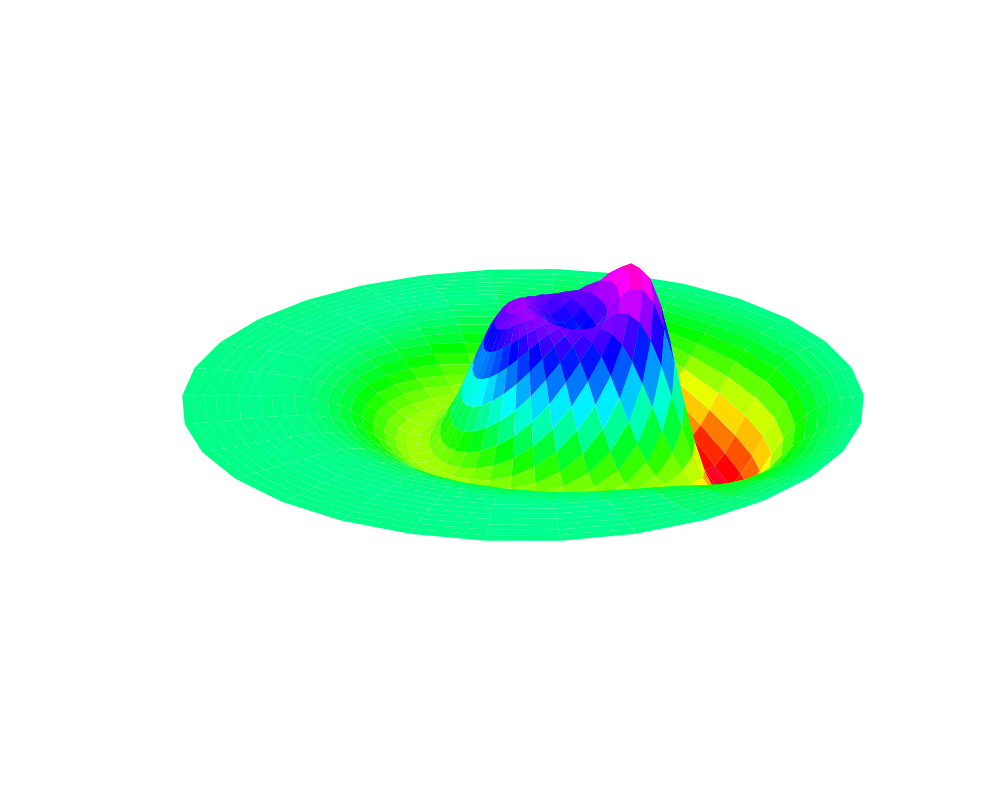
\includegraphics[scale=0.6]{Figures/circMembrane}

%\vskip1truein
Lance J.\ Nelson

\vskip.4truein
Department of Physics
\end{adjustwidth}

\cleardoublepage
\thispagestyle{empty}

 \begin{adjustwidth}{}{-1.5in}
 \centering
 \vspace*{1in}
 \large
 {\huge PH385: Numerical Methods in Physics}
 \vskip.4truein

 Lance J.\ Nelson
 \bigskip

 Department of Physics

 \bigskip
 Brigham Young University--Idaho

 \vfill


 {\footnotesize $\copyright$ 2017 Lance J.\ Nelson
               Brigham Young University--Idaho}

 \vskip.5truein
 {\footnotesize \emph{Last Revised: \today}}
 \normalsize

 \end{adjustwidth}

\cleardoublepage
\phantomsection
\chapter*{Preface}

This is a lab notebook intended to give you experience with
uncertainty analysis, experimental methods, and numerical methods in
physics.  All text with a bold P designation (\textbf{P1.1} for
example) indicates a task to be done.  Usually this will involve
writing something in your lab notebook.  Please be as complete and
neat as possible.

Any tasks that requires a computer will be done using the Python
programming language.  You can obtain a free copy of Python \href{https://store.enthought.com/downloads/}{here}.  
Any computer code that you create should be uploaded to the Google
Drive folder provided.

There is a companion book to this one entitled, ``Introduction to
Python''.  It is intended to help you learn to use Python to do the
tasks contained herein.  


 \cleardoublepage 
\phantomsection
 \addcontentsline{toc}{chapter}{Table of Contents}
\tableofcontents

\mainmatter
\renewcommand{\chaptermark}[1]{\markboth{Computational Physics 385}{\chaptername \ \thechapter \ \ #1}}
\chapter{A short introduction to \LaTeX}
As a scientist (or engineer), one of your most important tasks will be
to produce quality written documents detailing your work.  The quality
of the document that has your name attached to it speaks volumes about
the type of professional you are.  \LaTeX ~is your best friend in this
arena.  

You can think of \LaTeX ~as almost like a programming language for
generating documents.  You can create variables, loops, function, and
even use if/else statements, all in the context of document
production.  We won't focus on the most complicated parts of \LaTeX~
here but if you are interested, please come and talk to me.  At first
glance, \LaTeX ~may seem like a complicated version of Microsoft Word, but as
you gain experience using it you will find that it actually simplifies
many complicated tasks.  It is an especially useful tools when:
\begin{enumerate}
\item Your document contains a lot of math equations and you are
  referring to those equations frequently in the body of your document.
\item Your document has a lot of citations and a bibliography.
\item Your document has a lot of figures/graphics and you are
  frequently referencing them in the body of your document.
\item You'd like to use your programming skills to build nifty
  automations when building a document.  Here are a few examples
\begin{enumerate}
\item When I build an exam, I include the questions and the solutions
  in the same document.  By modifying a single variable I can turn
  those solutions on to build the key and off to build the exam.
\item When I build a schedule/calendar, I have a file that lists the
  correct dates and other date-specific information.  When the
  schedule is built, the dates are read from the file.  If I need to
  modify the schedule, I simply modify the list of dates and
  recompile.
\end{enumerate}
\end{enumerate}
\LaTeX~ is used heavily in research environments and is a skill
that will be an asset to you.  

\labsection{Getting Started}
The first thing we ought to learn is how to create a simple document
using \LaTeX.  

\begin{enumerate}
\probtwo Open your editor and type the following into the
window and press the \verb!Typeset! button.

\lstset{language=TeX,keywordstyle=\color{black}}
\begin{Verbatim}
\documentclass{article}
\begin{document}
This is a new document.  I can type whatever I want and it will appear
in the body of the text
\end{document}
\end{Verbatim}
\end{enumerate}
 

\noindent\rule{5 in}{0.01 in}

You probably wouldn't use \LaTeX ~to produce a document this simple,
but at least you can see how simple documents are produced. Please
note that every document you produce must have these lines:
\begin{Verbatim}
\documentclass{article}
\begin{document}

\end{document}
\end{Verbatim}


\labsection{Math} The fun starts when you need to add math to your
document.  \LaTeX ~ is great when it comes to producing great-looking,
numbered math equations that can easily be referenced from within the
body of the text.  Literally any math symbol you could want can be
produced if you know the correct syntax.  A full listing of the syntax
for all of the math symbols will not be provided here but can be
easily found with the help of Google.  

There are several different ways that you may want to incorporate math
into your document.  You may just want to add a math equation in the
middle of a sentence

\begin{enumerate}
\probtwo Type the following into your editor window and press the \verb!Typeset! button.
\lstset{language=TeX,keywordstyle=\color{black}}
\begin{Verbatim}
\documentclass{article}
\begin{document}
To find the electric field, we need to evaluate the integral:
$\frac{1}{\alpha} \int_0^{10} \ln(2 x) dx$ and then take the limit as
$\alpha \rightarrow \infty$.
\end{document}

\end{Verbatim}
Take a second to look at the output and to digest the code.  Ask any
questions that you may have.
\end{enumerate}

\noindent\rule{5 in}{0.01 in}

\noindent Let me highlight a few things that you should have noticed:
\begin{enumerate}
\item When typing math in the middle of a sentence, you must enclose
  the math expression in \$ symbols.
\item Sub- and super- scripts are done just as you would expect.  If
  the sub- or super-script is longer than one character, you must
  enclose it in curly braces (\{\}).
\item Common math symbols can be easily produced if you know the
  syntax.  Here we see that \verb!\int! is the syntax for the integral
  symbol, \verb!\ln! is the syntax for $\ln$, and \verb!\frac{}{}! is
  the symbol for making fractions (\verb!{num \over denom}! also works).  The syntax for other commonly-used
  math symbols is provided in table \ref{tab:LatexMathSymbols}.
\item Greek letters can also be produced if you know the correct syntax.
  In this example we see that \verb!\alpha! is the syntax for
  $\alpha$.  The syntax for a few of the other common greek letters is
  given in table \ref{tab:LatexGreekLetters} 
\end{enumerate}

Sometimes the math that you want to write down is a little longer and
you'd like it to be on it's own line.  That's no problem in \LaTeX

\begin{enumerate}
\probtwo  Type the following into your editor windown and push the
\verb!Typset! button:
\lstset{language=TeX,keywordstyle=\color{black}}
\begin{Verbatim}
\documentclass{article}
\usepackage{amsmath} % Needed to use \eqref
\begin{document}
To find the electric field, we need to evaluate the integral:
\begin{equation}\label{eq:integralEquation}
 \frac{1}{\alpha} \int_0^{10} \ln(2 x) dx
\end{equation}

When we evaluate equation \eqref{eq:integralEquation}, we find that it
equals $0$ because $\alpha = \infty$.

\end{document}
\end{Verbatim}

\marginpar{\footnotesize\captionsetup{type=table}
  \vspace{-2.5in}
\begin{tabular}{p{1.05in}p{1.05in}}
\texttt{\textbackslash{}frac\{1\}\{5\}} & $\frac{1}{5}$\\ \\
\texttt{\textbackslash{}sqrt\{5\}} & $\sqrt{5}$\\ \\
\texttt{\textbackslash{}int} & $\int$\\ \\
\texttt{\textbackslash{}ln} & $\ln$\\ \\
\texttt{\textbackslash{}oint} & $\oint$\\ \\
\texttt{\textbackslash{}sum} & $\sum$\\ \\
\texttt{\textbackslash{}infty} & $\infty$\\ \\
\texttt{\textbackslash{}nabla} & $\nabla$\\ \\
\texttt{\textbackslash{}partial} & $\partial$\\ \\
\end{tabular}
\captionof{table}{Commonly-used \LaTeX ~math symbols.\label{tab:LatexMathSymbols}}
}
 Take a second to look at the
output and to digest the code.  Ask any questions that you may have.

\noindent\rule{4.5 in}{0.01 in}
\end{enumerate}
\noindent Once again, let me highlight a few things that you should have noticed:
\begin{enumerate}
\item When you want an equation to be numbered and located on it's own
  line you can use the 
\begin{Verbatim}
\begin{equation} \label{myLabel}
<equation>
\end{equation}
\end{Verbatim} 
\item The \verb!\label! command can be used to assign a name to your
  equation.
\item You can use the name you gave to your equation to reference it
  in the text.  This means that you don't need to know the number that
  it was assigned.  This is done like this
  \verb!\eqref{equationLabel}!. Some commands require that you import
  an external package.  In this case, the \verb!\eqref! command needed
  the \verb!amsmath! package.
\end{enumerate}

Often you will have multiple lines of math and you want to be very
careful about how the lines line up.  Let's explore that a little
bit.

\marginpar{\footnotesize\captionsetup{type=table}
  \vspace{-2.5in}
\begin{tabular}{p{1.05in}p{1.05in}}
\texttt{\textbackslash{}alpha} & $\alpha$\\ \\
\texttt{\textbackslash{}beta} & $\beta$\\ \\
\texttt{\textbackslash{}gamma} & $\gamma$\\ \\
\texttt{\textbackslash{}chi} & $\chi$\\ \\
\texttt{\textbackslash{}Delta} & $\Delta$\\ \\
\end{tabular}
\captionof{table}{Commonly-used greek letters in \LaTeX.\label{tab:LatexGreekLetters}}
}

\begin{enumerate}
\probtwo  Type the folowing into the editor window and press the
\verb!Typeset! button \sidenote{A copy/paste may save you some time.}
\lstset{language=TeX,keywordstyle=\color{black}}
\begin{Verbatim}
\documentclass{article}
\usepackage{amsmath}
\begin{document}

\begin{equation}\label{kRadius}
k = \sqrt{\frac{2mE_f}{\hbar^2}}
\end{equation}

Now we can re-arrange to solve for $E_f$:

\begin{align}
3 \pi^2 \frac{N}{V} &= \left(\frac{2 m E_f}{\hbar^2}\right)^{3/2}\\
3 \pi^2 n &= \left(\frac{2 m E_f}{\hbar^2}\right)^{3/2}\\
\left(3 \pi^2 n\right)^{1/3} &= \left(\frac{2 m E_f}{\hbar^2}\right)^{1/2}\\
\left(3 \pi^2 n\right)^{1/3} &= \sqrt{\frac{2 m E_f}{\hbar^2}}\\
\end{align}

Comparing to equation \eqref{kRadius} we can conclude that:

\begin{equation}
k = \left(3 \pi^2 n\right)^{1/3}
\end{equation}


\end{document}
\end{Verbatim}
As before, digest what you see and ask any questions that you may
have.  What useful bits of information can you extract from this example
\end{enumerate}

\noindent\rule{5 in}{0.01 in}

These are just a few ways to produce math equations in your document.
As you progress in your abilities, more questions will undoubtedly
arise.  We'll handle those situations case by case in this class.
In conclusion, \LaTeX ~produces beautiful math that is formatted in
exactly the way that you want it and can be easily referenced from
within the text.  It should be your go-to tool anytime you need to
produce a document with math in it.

\labsection{Figures}
A key element of any scientific document are graphics.  This could be
a plot or a chart, or just an image.  Regardless, we need to figure
out how to include them in our \LaTeX ~ document.
\begin{enumerate}
\probtwo Download a picture of an elephant and save it to your
computer.  Then type the folowing into the editor window and press the
\verb!Typeset! button \sidenote{A copy/paste may save you some time.}
\sidenote{You may have to fiddle with the \texttt{scale=1.2} to get an
  appropriate size.}
\lstset{language=TeX,keywordstyle=\color{black}}
\begin{Verbatim}
\documentclass{article}
\usepackage{graphicx}  % You need this anytime you want to include graphics
\begin{document}

In figure \ref{figLabel} you will find an image of an elephant.
\begin{figure}
\includegraphics[scale = 1.2]{path/to/figure/of/elephant}
\caption{This is the caption to the figure \label{figLabel}}
\end{figure}

\end{document}
\end{Verbatim}
Look over the code and the output until things start to make sense.
Ask any questions that you may have.
\end{enumerate}

\noindent\rule{5 in}{0.01 in}
\noindent Once again, let me highlight a few things that you should have noticed:
\begin{enumerate}
\item Anytime you are including graphics in your document you will
  need the \verb!graphicx! package.
\item Including a graphic is done with the \verb!\includegraphics!
  command.  The \ul{required} argument to this function (found in curly
  braces) is the path to the image file.  One of the \ul{optional} arguments
  (found in square brackets) is \verb!scale = 1.2!, which allows you
  to specify the size of the image.
\item To label a figure (for referencing in the text) and creating
  captions you need to place your \verb!\includegraphics! statement in
\begin{Verbatim}
\begin{figure}

\end{figure}
\end{Verbatim}
\end{enumerate}


\labsection{Citations and Bibiliography}
A key element to any scientific paper are citations and a
bibliography page.  It is not uncommon for a published paper to have 30-40
citations.  Tracking and managing all of these citations manually
would be a mind-numbing task. Luckily, \LaTeX ~can handle all of this
for you.  There are two things that need to be discussed regarding
citations: i) finding the information for a source to be cited, ii)
citing a source and creating the bibliography.\\

\subsection*{Finding source information}
%\textbf{\Large Finding source information}
Google Scholar is a great place to do literature searches and it can
help you gather the bibliography information too.  But there are some
settings that need to be altered.
\begin{enumerate}
\probtwo  Follow the steps below to enable tex-friendly citation
information:
\begin{enumerate}
\item Go to www.google.com/scholar
\item In the upper left corner, click the drop down menu and click on
  \verb!Settings!.
\item Under Bibliography manager, click ``Show link to import
  citations into BibTeX'' and click ``Save''
\item Perform a search for ``Superalloys'', or some other interesting
  topic of your choosing.
\item Near the bottom of the first hit, there should be a link
  entitled ``Import into BibTex''.  Click it.  This is the source
  information that you will need
\end{enumerate}
\end{enumerate}
%\end{enumerate}
\subsection*{Citing a source and creating the bibliography}
For a scientist that is actively and frequently publishing papers, it
is quite common for them to cite the same source(s) in multiple
publications.  To simplify the citation process, a file that contains
all of his frequently-cited sources (commonly referred to as a ``bib''
file) is maintained.  

\begin{enumerate}
\probtwo Follow the steps below to create a simple bib file.
\begin{enumerate}
\item Create a new file named \texttt{refs.bib}.  It needs to
have the \texttt{.bib} postfix.  
\item Using Google Scholar, search for a few publications and copy
  their bibTex entry into the file refs.bib. (See previous section)  My refs.bib looks like
  this:
\lstset{language=TeX,keywordstyle=\color{black}}
\begin{Verbatim}
@article{caron2000high,
  title={High ysolvus new generation nickel-based superalloys for single crystal turbine blade applications},
  author={Caron, P},
  journal={Superalloys},
  volume={2000},
  pages={737--746},
  year={2000}
}

@article{pettit1984oxidation,
  title={Oxidation and hot corrosion of superalloys},
  author={Pettit, FS and Meier, GH and Gell, M and Kartovich, CS and Bricknel, RH and Kent, WB and Radovich, JF},
  journal={Superalloys},
  volume={85},
  pages={65},
  year={1984}
}

@article{pollock2006nickel,
  title={Nickel-based superalloys for advanced turbine engines: chemistry, microstructure, and properties},
  author={Pollock, Tresa M and Tin, Sammy},
  journal={Journal of propulsion and power},
  volume={22},
  number={2},
  pages={361--374},
  year={2006}
}

\end{Verbatim}
\item Save the file
\item Create another file in the same directory as the bib file.  Put
  the following into the file
\lstset{language=TeX,keywordstyle=\color{black}}
\begin{Verbatim}
\documentclass{article}
\begin{document}

As I discuss superalloys I may need to make a citation
\cite{pollock2006nickel}, or maybe even two at a time \cite{pettit1984oxidation,caron2000high}.

\bibliographystyle{ieeetr}  % There are various styles to choose from.
\bibliography{refs}
\end{document}
\end{Verbatim}
\end{enumerate}
\sidenote{The names of your citations will likely be different from
  mine.  You are also free to modify the names in the refs.bib file to
be whatever you want.}
Study the code and the output until things make sense.  Ask any
questions that you may have.
\end{enumerate}

\noindent\rule{5 in}{0.01 in}

\labsection{Miscellaneous}
The possible topics relating to \LaTeX~ functionality fills entire
books.  I will not try to be complete in my coverage.  Rather, let me
give you a few more handy tidbits that come up frequently.  Below you
will find 

\subsection*{Section Headings}
When organizing a document, you will want to use sections and
subsections. Here's how to do it.
\begin{Verbatim}
\section{Name of Section}  % Section with numbering
\subsection{Name of Subsection} % Subsection with numbering
\section*{Name of Section}  % Section with no numbering
\subsection*{Name of Subsection} % Subsection with no numbering

\end{Verbatim}

As mentioned in the comments, adding a * will supress the numbering
of the sections.
\pagebreak
\subsection*{Abstract and Title}
Every scientific document has an abstract, or short summary, of the
document.  Beneath the title of every paper is listed the authors
names and affiliations.  Here is how all of this is generated in
latex: 

\lstset{language=TeX,keywordstyle=\color{black}}
\begin{Verbatim}

\documentclass{article}
\usepackage{authblk}

            \title{The effect of variable air density on the trajectory of a cannon shell.}
            \author[1]{Lance J. Nelson}
            \affil[1]{Brigham Young University - Idaho}
            \author[2]{SECONDARY AUTHOR}
           \affil[2]{SECONDARY AUTHOR affiliation}
            \date{\today}
\begin{document}
    \maketitle
    \begin{abstract}
      Most projectile motion problems assume that the air density remains
      constant for the duration of the motion.  This is not a bad
      asssumption when the projectiles maximum altitude is relatively
      small.  However, for high altitude projectiles this may be a poor
      assumption.  In this work, we will investigate how a variable air
      density changes the trajectory of a high-altitude projectile.  We
      will also explore the effect of ground temperature on the range of
      these projectiles.
    \end{abstract}


This is my article


\end{document}
\end{Verbatim}
\pagebreak
\subsection*{Including code in your document}
In this class, you may want to include some or all of your code and
explain what you did.  Instead of copying your code into \LaTeX~
(ughh), \LaTeX~ can read your code file and place it into the
document, complete with text highlighting specific to the language you
are coding in.  Here is how you do it: \sidenote{Pay special attention
  to the comments for help understanding}

\begin{Verbatim}
\documentclass{article}
\pdfoutput=1

\usepackage{fancyvrb}
\usepackage{color}

\definecolor{purple}{rgb}{0.625,0.125,0.9375}
\usepackage{listings}
\lstset{
  frame=lines,  % top and bottom rule only
  framesep=2em, % separation between frame and text
    keepspaces=true,
    aboveskip=0in,
    belowskip=0.2in,
    language=Python, % What language are you coding in
    fancyvrb=true,
    breaklines=false,
    basicstyle=\footnotesize\ttfamily,
    numbers=left,
    stepnumber=1,
    keywordstyle=\color{blue},  %What color for keywords
    identifierstyle=,
    commentstyle=\color{red}, % What color do you want comments.
    stringstyle=\ttfamily\color{purple},
    columns=fullflexible,
    showstringspaces=False,
    caption = {  The following is an example code},  
    captionpos = b  % Where do you want the caption located
    }

\begin{document}


\lstinputlisting{testPython.py}  % This is where you specify
                                 % the location of your code file.
\end{document}

\end{Verbatim}

To say that we have only scratched the surface of what \LaTeX can do
would be a huge understatement.  However, what we have given you will
suffice for the requirements of this class.  If your curiosity
overwhelms you and you must have more, please feel free to come talk
with me one-on-one.


\labsection{Homework}



\begin{enumerate}
  \prob Recreate the document called exampleWriteUp.pdf found on
  iLearn.  The figures used in the document are also found on
  iLearn. You are free to use copy/paste to help speed up the process.
Note:  Use the document class
\verb!\documentclass[twocolumn]{revtex4-1}!  to make your document
look like mine.
Also note that all references to equations and figures must not be
hard-coded, but referenced using the assigned name.


\end{enumerate}
\lstset{language=Python,keywordstyle=\color{blue}}

\chapter{A short introduction to Python}
%\addcontentsline{toc}{chapter}{Review}
One goal of this class is that you become proficient with Python in a
scientific setting.  This will not happen all at once, but gradually
over the course of the entire semester.  You have already been exposed
to python in PH295 (previously PH291) but if you are like most
students, you might have struggled with loops, logic and functions.
These basic programming concepts are pretty crucial in this class.  In
this chapter, we'll review some python syntax and practice with some problems.

\labsection{Data Types} The most commonly used types of data that will
be used for this class are: integers, floats, strings, lists, and
arrays.  

\ul{Read sections 3.1 -- 3.6} in the Python manual to learn
  about the first four data types and \ul{sections 5.1--5.3} to learn
  about arrays.  If something you read is confusing or unfamiliar to
  you, I suggest that you try to recreate the calculation yourself.
  Take good notes so you can ask good questions during class.

Try the problem belwo to test your ability
\begin{enumerate}
\probtwo 

\item Build an array containing all multiples of 3 starting at 3 and
  ending at 2000.
\item Calculate $3 x^2 \sin(x) + \ln(x)$, where $x$ is the list you
  just created.  In other words, for every number in the array you
  just created, calculate the quantity above.  This will yield an
  array of calculated values.
\item Sum the elements of the list to get a single final answer.  
\end{enumerate}
Ans: -736905.545292\\
\ifsolutions
\textit{Solution:}\\
\begin{codeexample}
\begin{VerbatimOut}{\listingFile}
from numpy import arange,sin,log

x = arange(3,2000,3)
y = 3 *x**2 *sin(x) + log(x)
result = sum(y)

print result
\end{VerbatimOut}
\end{codeexample}
\else
\noindent\rule{5 in}{0.01 in}
\fi


\labsection{Loops and Logic} A loop is a set of instructions to be
performed until some pre-determined criteria is satisfied.  Loops are
used heavily in this class and you must grasp what they are as soon as
possible.  Logic refers to the act of checking the truthfulness of a
statement and is used heavily in conjunction with loops.

\ul{Read chapter 6 in the Python manual} to get a
better feel for what we mean. If something you read is confusing
  or unfamiliar to you, I suggest that you try to recreate the
  calculation yourself.  Take good notes so you can ask good questions
  during class.

Try the following problem to test your understanding of \texttt{for} loops
\begin{enumerate}
\probtwo On iLearn, you will find a file entitled ``massdata.txt''
which contains the mass of a collection of objects and their $(x,y,z)$
coordinates.
\begin{enumerate}
\item In Python, read in the data from the file (see chapter 8 in the python book).
\item Use a 'for' loop to loop over the data points and calculate the
  center of mass coordinates for the collection of particles.  You may
  remember that the equation find the center of mass is
\[x_\mathrm{cm} = {1\over M}\sum_i^N x_i m_i\]
\end{enumerate} 
\ifsolutions
\textit{Solution:}\\
\begin{codeexample}
\begin{VerbatimOut}{\listingFile}
with open('massdata.txt', 'r') as f:
    data = f.readlines()

masses = [x.split()[3] for x in data]

totalMass = sum(masses)
xCM = 0
yCM = 0
zCM = 0
for dPoint in data:
    x = float(dPoint.split()[0])
    y = float(dPoint.split()[1])
    z = float(dPoint.split()[2])
    m = float(dPoint.split()[3])
    xCM += x * m
    yCM += y * m
    zCM += z * m

xCM /= totalMass
yCM /= totalMass
zCM /= totalMass
print(xCM, yCM,zCM)
\end{VerbatimOut}
\end{codeexample}
\else
\noindent\rule{5 in}{0.01 in}
\fi
\end{enumerate}
Try the following problem to test your understanding of \texttt{while}
loops
\begin{enumerate}

    \probtwo Perform the summation below
    \[
        \sum_{n=1}^{\infty} n x^n
    \]
    using a {\tt while} loop.  Make your own counter for $n$ by using $n=0$
    outside the loop and $n=n+1$ inside the loop. Have the loop
    execute until the current term in the sum, $n x^n$ has dropped
    below $10^{-8}$. Verify that the sum only converges for $|x| < 1$
    and that when it does converge, it converges to
    $x/(1-x)^2$.\\
 Caution:  When building \texttt{while} loops, you can
    easily get caught in an infinite loop, one that never ends.  It's
    always wise to build in a fail safe: A variable to count the
    number of iterations and that breaks out of that loop if the
    number gets too high.\\
\ifsolutions
\textit{Solution:}\\
\begin{codeexample}
\begin{VerbatimOut}{\listingFile}
x = 0.75
thesum = 0
n = 1
while n * x**n > 1e-9:
    thesum += n * x**n 
    n = n + 1
    if n > 10000:
        break

checkVal = x /(1 -x)**2
print thesum, checkVal
\end{VerbatimOut}
\end{codeexample}
\else
\noindent\rule{5 in}{0.01 in}
\fi
\end{enumerate}

%Write a {\tt for}
%    loop that counts by threes starting at 2 and ending at 101.
%    Along the way, every time you encounter a multiple of 5 print
%    a line that looks like this (in the printed line below it
%    encountered the number 20.)\\
%\begin{Verbatim}
%fiver: 20
%\end{Verbatim}
%    You will need to use the modulo opertor({\tt \%}) to check for multiples of 5.
%\ifsolutions
%\textit{Solution:}\\
%\begin{codeexample}
%\begin{VerbatimOut}{\listingFile}
%for i in range(2,101,3):
%    if i % 5 == 0:
%        print "fiver:", i
%\end{VerbatimOut}
%\end{codeexample}
%\else
%\noindent\rule{5 in}{0.01 in}
%\fi


\labsection{Functions} A function is like a black box.  The user
passes some needed information into the box and the box uses that
information to perform some useful calculation and spits a result
out.  

\ul{Read chapter 4} in the Python manual to see how to
  build functions in Python. If something you read is confusing or
  unfamiliar to you, I suggest that you try to recreate the
  calculation yourself.  Take good notes so you can ask good questions
  during class.

Try the following problem to test your abilities
\begin{enumerate}

    \probtwo Build a function that contains a loop that sums the integers
    from 1 to $N$, where $N$ is an integer value that is passed into
    the function. By calling the function at least 5 times, verify
    that the formula
    \[
        \sum_{n=1}^N n = \frac{N(N+1)}{2}
    \]
    is correct.\\
\ifsolutions
\textit{Solution:}\\
\begin{codeexample}
\begin{VerbatimOut}{\listingFile}
def loopFunction(N):
    thesum = 0
    for i in range(1,N+1):
        thesum += i

    return thesum

N = 100
loopVal = loopFunction(N)
checkVal = N * (N + 1)/2.
print loopVal, checkVal
\end{VerbatimOut}
\end{codeexample}
\else
\noindent\rule{5 in}{0.01 in}
\fi
\end{enumerate}
\labsection{Plotting} \textbf{Computers can't plot
  functions}. Computers can only evaluate functions and plot data
points.  If you choose to evaluate a function on a very dense grid of
points, plot those points, and connect them with a line, the resulting
plot will resemble the function.  This way of
thinking will be increasingly important as the semester progresses.
\ul{Read chapter 7} in the Python manual to get a better
  idea of how to construct a plot in Python. If something you read is
  confusing or unfamiliar to you, I suggest that you try to recreate
  the calculation yourself.  Take good notes so you can ask good
  questions during class.

\begin{enumerate}
    \probtwo Plot the function 
    \[
        y(x) = e^{-0.25 x} \cos(x)
    \]

from $ x = 0$ to $x = 10$.\\
\ifsolutions
\textit{Solution:}\\
\begin{codeexample}
\begin{VerbatimOut}{\listingFile}
from numpy import arange, e, cos
from matplotlib import pyplot
x = arange(0,10,.1)
y = e**(-0.25 * x) * cos(x)
pyplot.plot(x,y)
pyplot.show()
\end{VerbatimOut}
\end{codeexample}
\else
\noindent\rule{5 in}{0.01 in}
\fi
\end{enumerate}
\labsection{Classes} You can think of a class as an object that
contains both data and functions.  Since you are already familiar with
variables and functions, the best way to learn about classes is to see
one and then ask questions. Here is a simple class used to
analyze ideal gas processes:
\begin{Verbatim}
class idealGas():
    def __init__(self,R=8.314,kB=1.38e-23):
        self.R = R
        self.kB = kB
    
    #Define what kind of ideal gas process we are dealing with
    def setProcessType(self,process, n,cV):
        self.n = n  #Set the number of moles of the gas
        self.process = process  #Indicate what kind of process it is:
                                # Isothermal, Isobaric, Adiabatic, Isochoric
        self.cV = cV
        self.cP = self.cV + self.R
        # If the process is adiabatic, we might need to know what gamma is.
        if process == 'Adiabatic':  
             self.gamma = self.cP/self.cV

    # Set the initial and final conditions for the process.
    def setConditions(self,pi=None,Vi=None,Ti=None,pf=None,Vf=None,Tf=None):
        self.pi = pi
        self.Vi = Vi
        self.Ti = Ti
        self.pf = pf
        self.Vf = Vf
        self.Tf = Tf

    def isothermal(self):
        from math import log
        self.work = -self.n * self.R * log(self.Vf/self.Vi)
        self.deltaE = 0
        self.heat = - self.work
        
    def isochoric(self):
        self.work = 0
        self.heat = self.n * self.cV * (self.Tf - self.Ti)
        self.deltaE = heat
        
    def isobaric(self):
        self.work = - self.pI * (self.Vf - self.Vi)
        self.heat = self.n * self.cP * (self.Tf - self.Ti)
        self.deltaE = self.n * self.cV * (self.Tf - self.Ti)
        
    def adiabatic(self):
        self.heat = 0
        self.deltaE = self.n * self.cV * (self.Tf - self.Ti)
        self.work = self.deltaE

    # Depending on what type of process it is, calculate the work
    # done, heat absorbed, and change in internal energy for the process.
    def calculate(self):

        
        # These three lines can replace the lines below and its a really
        # cool use of dictionaries. Try it.
        #         processes = {'Isothermal':self.isothermal, 'Adiabatic':
        #   self.adiabatic, 'Isochoric':self.isochoric, 'Isobaric':self.isobaric}
        # processes[self.process]()

         if self.process == 'Isothermal':
             self.isothermal()
         elif self.process == 'Isochoric':
             self.isochoric()
         elif self.process == 'Isobaric':
             self.isobaric()
         else:  #Adiabatic
             self.adiabatic()

# Class definition done. What follows below illustrates how to use the class.
gasOne = idealGas()  #Initialize the class.
gasOne.setProcessType('Isothermal',3,20.8)  # Set the type of process and number of moles
gasOne.setConditions(pi = 2.0e5, pf = 1.0e5,Ti = 200, Tf = 200, Vi = 2, Vf = 5 )  # Set initial and final conditions
gasOne.calculate()  # Calculate thermodynamic properties.
print(gasOne.work)  # Print results
print(gasOne.deltaE)

\end{Verbatim}
\labsection{Homework}

\begin{enumerate}
    \prob Build a function that takes argument $x$ and performs the sum
    \[
        \sum_{n=1}^{1000} n x^n
    \]
    using a {\tt for} loop.  By calling the function with different
    values of $x$, verify that the sum only converges for $|x| < 1$
    and that when it does converge, it converges to $x/(1-x)^2$.\\
\ifsolutions
\textit{Solution:}\\
\begin{codeexample}
\begin{VerbatimOut}{\listingFile}
def loopFunction(x):
    thesum = 0
    for n in range(1,1001):
        thesum += n * x**n 

    return thesum

x = 0.75
loopVal = loopFunction(x)
checkVal = x /(1 -x)**2
print loopVal, checkVal
\end{VerbatimOut}
\end{codeexample}
\else
\noindent\rule{5 in}{0.01 in}
\fi

%    \index{While loop} \index{Loops!while} 
%
%    \prob Redo the previous exercise using a {\tt while} loop instead
%    of a {\tt for} loop.  Make your own counter for $n$ by using $n=0$
%    outside the loop and $n=n+1$ inside the loop. Have the loop
%    execute until the current term in the sum, $n x^n$ has dropped
%    below $10^{-8}$. Verify that this way of doing it agrees with what
%    you found in the previous exercise.\\
%\ifsolutions
%\textit{Solution:}\\
%\begin{codeexample}
%\begin{VerbatimOut}{\listingFile}
%def loopFunction(x):
%    thesum = 0
%    n = 1
%    while n * x**n > 1e-9:
%        thesum += n * x**n 
%        n = n + 1
%    return thesum
%
%x = 0.75
%loopVal = loopFunction(x)
%checkVal = x /(1 -x)**2
%print loopVal, checkVal
%\end{VerbatimOut}
%\end{codeexample}
%\else
%\noindent\rule{5 in}{0.01 in}
%\fi

%\prob Verify by numerical experimentation with a {\tt while}
%    loop that
%    \[
%        \sum_{n=1}^{\infty} \frac{1}{n^2} = \frac{\pi^2}{6}
%    \]
%    Set the {\tt while} loop to quit when the next term added to
%    the sum is below $10^{-6}$.

\prob Verify, by numerically experimenting with a 
    loop that uses the {\tt break} command to
    exit the loop at the appropriate time, that the
    following infinite-product relation is true:
    \[
        \prod_{n=1}^{\infty} \left( 1 + \frac{1}{n^2} \right)
        = \frac{ \sinh{\pi} }{ \pi }
    \]\\
\ifsolutions
\textit{Solution:}\\
\begin{codeexample}
\begin{VerbatimOut}{\listingFile}
from numpy import sinh,pi

n = 1.
theproduct = 1.
while 1/n**2 > 1e-10:
    theproduct *= 1 + 1/n**2
    n += 1

print theproduct
print sinh(pi)/pi
\end{VerbatimOut}
\end{codeexample}
\else
\noindent\rule{5 in}{0.01 in}
\fi


\prob \index{Iteration} \index{Successive substitution}(\textbf{Transcendental
Equations})  A transcendental equation is one that cannot be solved
analytically.  Try solving the following equation for
$x$:
\[{\sin(x)\over x} = 1\]
to see what I mean.  One numerical method for solving this kind of
problem involves first rearranging the equation to look like this:
\[x = \sin(x)\] and then repeatedly evaluating the r.h.s using the
result of the previous evalution until subsequent evaluations differ
very little. \sidenote{This method is called successive evaluation}

Use a {\tt while} loop to verify that the following three iteration
    processes converge. Execute the loops
    until convergence at the $10^{-8}$ level is achieved.
    \[
        x_{n+1} = e^{-x_n}~~~~;~~~~
        x_{n+1} = \cos{x_n}~~~~;~~~~
        x_{n+1} = \sin{2 x_n}
    \]
    Note: iteration loops are easy to write. Just give $x$ an initial
    value (any number will do) and then inside the loop replace $x$ by
    the formula on the right-hand side of each of the equations
    above. To watch the process converge you will need to call the new
    value of $x$ something like {\tt xnew} so you can compare it to
    the previous $x$.

    Finally, try iteration again on this problem:
    \[
        x_{n+1} = \sin{3 x_n}
    \]
    Convince yourself that this process isn't converging to
    anything. We will see in Lab~\ref{Lab:19} what makes the
    difference between an iteration process that converges and
    one that doesn't.\\
\ifsolutions
\textit{Solution:}\\
\begin{codeexample}
\begin{VerbatimOut}{\listingFile}
from numpy import arange,sin,log,exp,cos

x = 100   # Set initial value
xNew = sin(3 * x)  # Find next value

while abs(x - xNew) > 1e-8:
    x = xNew  # Update old value to be what you just found
    xNew = sin(3 * x)  # Find the next value
    print xNew

\end{VerbatimOut}
\end{codeexample}
\else
\noindent\rule{5 in}{0.01 in}
\fi


\prob Write a class to calculate the trajectory of a projectile.  You should
have at least three member functions to: i) set the launch conditions (initial
velocity, position, etc.  ii) calculate the landing location and iii)
plot the trajectory.
\end{enumerate}

%\mainmatter

%\pagestyle{fancy}
%\renewcommand{\chaptermark}[1]{\markboth{Computational Physics 385}{\chaptername \ \thechapter \ \ #1}}
\footcite{giordano1997computational}
\part{Preliminaries}
\chapter[Discrete Grids]{Discrete Grids}
\label{ch:grids}
%\addcontentsline{toc}{chapter}{Grids and Derivatives}
\begin{center}
\textbf{Python skills that you will need for today:\\
    Plotting (Chapter 7), numpy array construction (section 5.3)}
\end{center}

Analytical solutions to differential equations yield analytic
functions; functions that can be evaluated at arbitrary
points. Transitioning from analytical solutions to differential
equations to numerical solutions requires a shift in mentality.  When
you solve a differential equation numerically, the solution function
is represented as an array of function values on a discrete grid.  It
is important now to develop the intuition and skills for representing
a function as a discrete set of values on a grid.  Before we proceed to
solving differential equations, let's spend some time getting
comfortable working with spatial grids.

\marginfig[-1in]{Figures/f01Grids}{\label{f01Grids}Three common spatial grids}

\labsection{Spatial grids}

Figure~\ref{f01Grids} shows a graphical representation of three
types of spatial grids for the region $0 \le x \le L$.  We divide
this region into spatial \emph{cells} (the spaces between vertical
lines) and functions are evaluated at $N$ discrete \emph{grid
points} (the dots). In a \emph{cell-edge} grid,\index{Cell-edge
grid}\index{Grids!cell-edge} the grid points are located at the
edge of the cell.  In a \emph{cell-center} grid,\index{Cell-center
grid}\index{Grids!cell-center} the points are located in the middle
of the cell.  Another useful grid is a cell-center grid with {\it
ghost points}.\index{Ghost points} The ghost points (unfilled dots)
are extra grid points on either side of the interval of interest
and are useful when we need to consider the derivatives at the edge
of a grid.


%\begin{example}
%
% Make a Python script that creates a
%  cell-edge spatial grid in the variable {\tt x} over the interval $0 \le x \le \pi$ with $N=500$.
%  \marginfig{Figures/f01p1a}{Plot from \ref{P:1.1a}} 
%    Plot the function $y(x) = \sin(x) \sinh(x)$ on this grid.
%    Explain the relationship between the number of cells and
%    the number of grid points in a cell-edge grid. Then
%    verify that the number of points in this $x$-grid is $N$
%    (using Python's {\tt len} command).
%
%\textit{Solution:}\\
%\begin{codeexample}
%\begin{VerbatimOut}{\listingFile}
%from numpy import linspace,pi,sin,sinh  # Import the needed function
%from matplotlib import pyplot
%N=500             # the number of grid points
%a=0
%b=pi          # the left and right bounds
%x=linspace(a,b,N)           # build the grid
%print(x)
%y = sin(x) * sinh(x)
%print(len(x))
%pyplot.plot(x,y)
%pyplot.show()
%\end{VerbatimOut}
%\end{codeexample}
%\end{example}
\begin{enumerate}
\probtwo \label{P:1.1}
\begin{enumerate}
  \subprob \label{P:1.1a} Make a Python script that creates a
  cell-edge spatial grid in the variable {\tt x} over the interval $0 \le x \le \pi$ with $N=500$.
  \marginfig{Figures/f01p1a}{Plot from \ref{P:1.1a}} 
    Plot the function $y(x) = \sin(x) \sinh(x)$ on this grid.
    Explain the relationship between the number of cells and
    the number of grid points in a cell-edge grid. Then
    verify that the number of points in this $x$-grid is $N$
    (using Python's {\tt len} command).\\
\ifsolutions
\textit{Solution:}\\
\begin{codeexample}
\begin{VerbatimOut}{\listingFile}
from numpy import linspace,pi,sin,sinh  # Import the needed function
from matplotlib import pyplot
N=500             # the number of grid points
a=0
b=pi          # the left and right bounds
x=linspace(a,b,N)           # build the grid
print x
y = sin(x) * sinh(x)
print len(x)
pyplot.plot(x,y)
pyplot.show()
\end{VerbatimOut}
\end{codeexample}
\else
\noindent\rule{4 in}{0.01 in}
\fi

    \subprob \label{P:1.1b} Now let's do a cell-centered grid.  Notice
    that your grid doesn't start at \texttt{a} or end at \texttt{b}.
    Rather, your grid starts at $a + \frac{dx}{2}$ and ends at $b -
    \frac{dx}{2}$, where $dx$ is the grid spacing.  This means that
    you will need to add a line that calculates the grid spacing.
    Think about this and add the needed line to calculate it.  Verify
    that your grid points are correct and that there are still $500$ of them.\\
\ifsolutions
\textit{Solution:}\\
\begin{codeexample}
\begin{VerbatimOut}{\listingFile}
from numpy import linspace, arange,pi,sin, sinh

from matplotlib import pyplot

a = 0
b = pi
N = 10.
dx = (b  - a)/ N  # grid seperation
print dx

x = arange(a+dx/2,b+dx/2,dx)
print x
y = sin(x) * sinh(x)
print y
print len(x)
pyplot.plot(x,y)
pyplot.show()
\end{VerbatimOut}
\end{codeexample}
\else
\noindent\rule{4 in}{0.01 in}
\fi
    \subprob Now write a script like the one in part (b) to build a cell-center
    grid over the interval $0 \le x \le 2$ with $N=5000$. Evaluate the
    function $f(x)=\cos{x}$ on this grid and plot this function. Then
    estimate the area under the curve by summing the products of the
    centered function values $f_j$ with the widths of the cells $h$
    like this (midpoint integration rule):
\begin{Verbatim}
sum(f)*h;
\end{Verbatim}

    Verify that this result is quite close to the exact
    answer obtained by integration:
    \[
        A=\int_0^2 \cos{x} ~dx.
    \]\\
\ifsolutions
\textit{Solution:}\\
\begin{codeexample}
\begin{VerbatimOut}{\listingFile}
from numpy import arange,cos
from matplotlib import pyplot

a = 0
b = 2
N = 5000.
dx = (b  - a)/ N  # grid seperation
print dx

x = arange(a+dx/2,b+dx/2,dx)
print x
y = cos(x)
print y
print len(x)
area = sum(y) * dx
print area
pyplot.plot(x,y)
pyplot.show()
\end{VerbatimOut}
\end{codeexample}
\else
\noindent\rule{4 in}{0.01 in}
\fi
\marginfig{Figures/f01p1b}{Plot from \ref{P:1.1b}}

\end{enumerate}
\end{enumerate}

%Python has a convenient command {\tt linspace} for building one
%dimensional grids.  The syntax for building a grid is
%\begin{Verbatim}
%x = linspace(a,b,N);
%\end{Verbatim}
%where {\tt a} is the $x$ position of the first point in the grid,
%{\tt b} is the $x$-position of the last point in the grid, and {\tt
%N} is the number of grid points.  This method doesn't give you the
%grid spacing back, but you can always calculate it by subtraction:
%\begin{Verbatim}
%h = x(2) - x(1);
%\end{Verbatim}
%Depending on what you choose for {\tt a} and {\tt b}, {\tt linspace}
%can give you either cell-edge or cell-center grids.

\labsection{Interpolation and extrapolation}
\index{Interpolation} \index{Extrapolation}

Grids only represent functions at discrete points, and there will be
times when we want to find good values of a function {\it between}
grid points (interpolation) or \emph{beyond} the last grid point
(extrapolation). We will use interpolation and extrapolation
techniques fairly often during this course, so let's review these
ideas.

\marginfig{Figures/f01Linear}{The line defined by two points can be used to
interpolate between the points and extrapolate beyond the points.}

The simplest way to estimate these values is to use the fact that two
points define a straight line. For example, suppose that we have
function values $(x_1,y_1)$ and $(x_2,y_2)$. The formula for a
straight line that passes through these two points is
\begin{equation} \label{eq:linear}
    y-y_1 = \frac{ (y_2-y_1) }{ (x_2-x_1) } (x-x_1)
\end{equation}
Once this line has been established it provides an approximation to
the true function $y(x)$ that is pretty good in the neighborhood of
the two data points. To linearly interpolate or extrapolate we simply
evaluate Eq.~(\ref{eq:linear}) at $x$ values between or beyond $x_1$
and $x_2$.

\begin{enumerate}
\probtwo \label{P:1.3} Use Eq.~(\ref{eq:linear}) to do the following
    special cases:

\begin{enumerate}
\subprob Find an approximate value for $y(x)$ halfway between
    the two points $x_1$ and $x_2$. Does your answer make
    sense?\\
\ifsolutions
\textit{Solution:}
\begin{equation}
x = x_1 + {1 \over 2} (x_2 - x_1)
\end{equation}
\begin{align}
    y-y_1 &= \frac{ (y_2-y_1) }{ (x_2-x_1) } (x_1 + {1 \over 2} (x_2 -
    x_1)-x_1)\\
y &= \frac{ (y_2-y_1) }{ (x_2-x_1) } ({1 \over 2} (x_2 -
x_1)) + y_1\\
y &= y_1 + {1 \over 2} (y_2-y_1) \\
\end{align}

\fi
\subprob Find an approximate value for $y(x)$ 3/4 of the way
    from $x_1$ to $x_2$. Do you see a pattern?\\
\ifsolutions
\textit{Solution:}
\begin{align}
x &= x_1 + {3\over 4}(x_2 - x_1)\\
\end{align}
\begin{align}
    y-y_1 &= \frac{ (y_2-y_1) }{ (x_2-x_1) } (x_1 + {3 \over 4} (x_2 -
    x_1)-x_1)\\
y &= \frac{ (y_2-y_1) }{ (x_2-x_1) } ({3 \over 4} (x_2 -
x_1)) + y_1\\
y &= y_1 + {3 \over 4} (y_2-y_1) \\
\end{align}

\fi

Note: You should find that 
\begin{equation}
y(x_1 + p h) = y_1 + p (y_2 - y_1)
\end{equation}
, where $p$ is a fraction of the grid spacing. (${1\over 2}$ for part
a and ${3\over 4}$ for part b.)
\subprob If the spacing between grid points is $h$ (i.e.
    $x_2-x_1=h$), show that the linear extrapolation formula
    for $y(x_2+h)$ is
    \begin{equation}\label{eq:linExtrap}
        y(x_2+h) = 2 y_2 - y_1
    \end{equation}
    This provides a convenient way to estimate the function
    value one grid step beyond the last grid point. \\ 
\ifsolutions
\textit{Solution:}
Start with equation \eqref{eq:linear}
\begin{align} 
    y-y_1 &= \frac{ (y_2-y_1) }{ (x_2-x_1) } (x-x_1)\\
y &= \frac{ (y_2-y_1) }{ h } (x_2 + h -x_1) + y_1\\
&= \frac{ (y_2-y_1) }{ h } (h  + h) + y_1\\
&= \frac{ (y_2-y_1) }{ h } 2h + y_1\\
&= 2(y_2-y_1) + y_1\\
&= 2y_2-2y_1 + y_1\\
&= 2y_2-y_1\\
\end{align}
\fi

\subprob Also show that
    \begin{equation}\label{eq:linExtraphalf}
        y(x_2+{ h\over 2}) = {3\over 2} y_2 - {1\over 2}y_1 .
    \end{equation}
    We will use both of these formulas during the course.\\
\ifsolutions
Start with equation \eqref{eq:linear}
\begin{align} 
    y-y_1 &= \frac{ (y_2-y_1) }{ (x_2-x_1) } (x-x_1)\\
y &= \frac{ (y_2-y_1) }{ h } (x_2 + {h \over 2} -x_1) + y_1\\
&= \frac{ (y_2-y_1) }{ h } (h  + {h\over 2}) + y_1\\
&= {3\over 2}(y_2-y_1) + y_1\\
&= {3\over 2} y_2- {3\over 2} y_1 + y_1\\
&= {3\over 2} y_2-{1\over 2} y_1\\
\end{align}

\fi
\noindent\rule{4 in}{0.01 in}

\end{enumerate}
\end{enumerate}

\marginfig{Figures/f01Quadratic}{Three points define a parabola that can be
used to interpolate between the points and extrapolate beyond the
points.}

A fancier technique for finding values between and beyond grid points
is to use a parabola instead of a line. It takes three data points to
define a parabola, so we need to start with the function values
$(x_1,y_1)$, $(x_2,y_2)$, and $(x_3,y_3)$. The general formula for a
parabola is
\begin{equation}\label{eq:Parabola}
    y=a + bx + cx^2
\end{equation}
where the coefficients $a$, $b,$ and $c$ need to be chosen so that
the parabola passes through our three data points. To determine these
constants, you set up three equations that force the parabola to
match the data points, like this:
\begin{equation}\label{eq:ParabolaSet}
    y_j = a + bx_j + cx_j^2
\end{equation}
with $j=1,2,3$, and then solve for $a$, $b$, and $c$.

\begin{enumerate}
\probtwo \label{P:1.4} Use Eq.~(\ref{eq:ParabolaSet}) to create a
    set of three equations in Mathematica. For simplicity, assume
    that the points are on an evenly-spaced grid and set
    $x_2=x_1+h$ and $x_3=x_1+2h$.  Solve this set of equations to
    obtain some messy formulas for $a$, $b$, and $c$ that involve
    $x_1$, $y_1$, $y_2$, $y_3$, and $h$. Then use these formulas to solve the following
    problems:

\begin{enumerate}

\subprob Estimate $y(x)$ half way between $x_1$ and $x_2$,
    and then again halfway between $x_2$ and $x_3$. Do you
    see a pattern? (You will need to simplify the answer that
    Mathematica spits out to see the pattern.)

\subprob Show that the quadratic extrapolation formula for
    $y(x_3+h)$ (i.e. the value one grid point beyond $x_3$)
    is
    \begin{equation}\label{eq:quadExtrap}
        y(x_3+h) = y_1 - 3 y_2 + 3 y_3
    \end{equation}
    Also find the formula for $y(x_3+h/2)$.
\ifsolutions
Answer:  You should find that the interpolated value between $x_1$ and
$x_2$ is
\begin{equation}
{1\over 8} \left( 3 y_1 + 6 y_2 - y_3\right)
\end{equation}
and the value in between $x_2$ and $x_3$ is
\begin{equation}
{1\over 8} \left( - y_1 + 6 y_2 + 3 y_3\right)
\end{equation}

\fi
\end{enumerate}
\end{enumerate}

\labsection{Homework}
\begin{enumerate}
\prob 
\begin{enumerate}
\item Build a cell-centered grid in the variable {\tt x} over the
interval $0 \le x \le \pi$ with $N=500$.
\item Evaluate the function $\sinh(x)$ on the grid.
\item Use linear extrapolation to determine the value of the function
  one grid point beyond the last one.  Compare to the true value of the
  function at that point.
\item Use quadratic extrapolation to determine the value of the function
  one grid point beyond the last one.  Compare to the true value of
  the function at that point.
\item Use linear interpolation to determine the value of the function
  between the last and second-to-last grid point.  Compare to the true
  value of the function.
\item Use quadratic interpolation to determine the value of the
  function between the last and second-to-last grid point.  Compare to
  the true value of the function.
\ifsolutions
\textit{Solution:}\\
\begin{codeexample}
\begin{VerbatimOut}{\listingFile}
from numpy import sinh,arange
from matplotlib import pyplot

a = 0
b = 2
N = 100.
dx = (b  - a)/ N  # grid seperation

x = arange(a+dx/2,b+dx/2,dx)
y = sinh(x)

yExtrapLinear = 2 * y[-1] - y[-2]
yExtrapQuad = y[-3] - 3 * y[-2] + 3 * y[-1]
yExtrapExact = sinh(x[-1] + dx)
print yExtrapLinear, yExtrapQuad, yExtrapExact
yInterpLinear =  y[-2] + 1/2. * (y[-1] - y[-2])
yInterpQuad = 1/8. * (-y[-3] + 6 * y[-2] + 3 * y[-1])
yInterpExact = sinh(x[-2] + dx/2.)
print yInterpLinear, yInterpQuad, yInterpExact
\end{VerbatimOut}
\end{codeexample}
\else
\noindent\rule{4 in}{0.01 in}
\fi
\end{enumerate}
\end{enumerate}

\chapter[Numerical Derivatives]{Numerical Derivatives}
\label{ch:numderivs}
%\addcontentsline{toc}{chapter}{Grids and Derivatives}

In calculus class (long ago now) you were taught analytical techniques
for calculating derivatives and integrals.  In other words, given a
function $f(x)$ you were taught how to find the function:
$\frac{df}{dx}$.  These techniques are great if you have $f(x)$ but
aren't very helpful if you don't.  In numerical physics you typically
don't have $f(x)$ but you probably have a way to gather samples from
$f(x)$.  How can we use these discrete function values to calculate
derivatives and integrals. This will be our topic for this chapter.

\labsection{Numerical Derivatives} \index{Derivatives, first and
  second} \index{Forward difference formula} 

In your introductory
calculus book, the derivative was probably introduced using the {\it
  forward difference} formula
\begin{equation}\label{eq:forwarddiff}
     f'(x) \approx \frac{f(x+h)-f(x)}{h} .
\end{equation}
The word ``forward'' refers to the way this formula reaches forward
from $x$ to $x+h$ to calculate the slope. The exact derivative
represented by Eq.~(\ref{eq:forwarddiff}) in the limit that $h$
approaches zero.  However, we can't make $h$ arbitrarily small when
we represent a function on a grid because (i) the number of cells
needed to represent a region of space becomes infinite as $h$ goes to
zero; and (ii) computers represent numbers with a finite number of
significant digits so the subtraction in the numerator of
Eq.~(\ref{eq:forwarddiff}) loses accuracy when the two function
values are very close. But given these limitation we want to be as
accurate as possible, so we want to use the best derivative formulas
available. The forward difference formula isn't one of them.

\marginfig{chapters/f01FiniteDifference}{The forward and centered difference
formulas both approximate the derivative as the slope of a line
connecting two points. The centered difference formula gives a more
accurate approximation because it uses points before and after the
point where the derivative is being estimated. (The true derivative
is the slope of the dotted tangent line).}

The best first derivative formula that uses only two function values
is usually the {\it centered difference} formula: \index{Centered
difference formula}
\begin{equation}\label{eq:CenteredDiff}
    f'(x) \approx \frac{f(x+h)-f(x-h)}{2h} .
\end{equation}
It is called ``centered'' because the point $x$ at which we want the
slope is centered between the places where the function is evaluated.
The corresponding centered second derivative formula is \index{Second
derivative}
\begin{equation}\label{eq:seconderivative}
    f''(x) \approx {f(x+h)-2 f(x)+f(x-h) \over h^2}
\end{equation}
You will derive both of these formulas a little later, but for now we
just want you to understand how to use them.


  To see the importance of centering, consider
  Fig.~\ref{figDerivatives}. In this figure we are trying to find the
  slope of the tangent line at $x=0.4$.  The usual calculus-book
  formula uses the data points at $x=0.4$ and $x=0.5$, giving tangent
  line $a$. It should be obvious that using the ``centered'' pair of
  points $x=0.3$ and $x=0.5$ to obtain tangent line $b$ is a much
  better approximation. \textbf{When approximating derivatives using
  finite difference we'll always want to use the centered difference
  (if possible).}
\marginfig{Figures/figDerivatives}{The centered derivative approximation works
    best.\label{figDerivatives}}

\begin{enumerate}
\probtwo  To experiment with the different numerical derivative
formulas and to see why the centered-difference is better, do the
following:
\begin{enumerate}
\item Differentiate $\sin(x)$ at $x=1$ using the forward-difference
  formula and the centered-difference formula.
\item The true value of the derivative is $\cos(1)$.  Compute the
  ratio of the numerical derivative with the true answer for both
  methods.
\item Can you see which method is better?
\end{enumerate}
\end{enumerate}
\ifsolutions
\textit{Solution:}\\
\begin{codeexample}
\begin{VerbatimOut}{\listingFile}
from numpy import linspace, sin,cosh, cos
from matplotlib import pyplot

h = 1e-5
forward = (sin(1 + h) - sin(1))/h
centered = (sin(1 + h) - sin(1 - h) ) /( 2 * h)
trueVal = cos(1)

print forward/trueVal, centered/trueVal
\end{VerbatimOut}
\end{codeexample}
\else
\noindent\rule{5 in}{0.01 in}
\fi

\labsection{Derivatives on Grids}
Equations \eqref{eq:CenteredDiff} and \eqref{eq:seconderivative} are
great for evaluating a derivative at a single point.  But what if we
have an entire array of function values and we'd like to evaluate the
derivative at all of the points.  In other words, what if we want to
determine the shape of the derivative function.
\ul{Luckily, when grids are stored in Numpy arrays}, the colon operator
provides a compact way to evaluate Eqs.~(\ref{eq:CenteredDiff}) and
(\ref{eq:seconderivative}) on a grid.  

\begin{enumerate}
\probtwo Perform the following to see how to compute a numerical
derivative of a grid of function values:\label{derivOnGrid}
\begin{enumerate}
\subprob Create a cell-edge grid with $N=100$ on the interval $0 \le x
    \le 5$.  Call the array \texttt{x}
\subprob For the grid that you just created, create an array of
function values for the following function: $\sin(x) \cosh(x)$.  Call
the array \texttt{y}.
\subprob \ul{Using only a single line of code}, evaluate the derivative of
the function that you just created. 
\subprob \ul{Using only a single line of code}, evaluate the second derivative of
the function that you just created. 
\subprob  Plot the original function and it's first derivative on the
same graph.
\end{enumerate}
\end{enumerate}
\ifsolutions
\textit{Solution:}\\
\begin{codeexample}
\begin{VerbatimOut}{\listingFile}
from numpy import linspace, sin,cosh
from matplotlib import pyplot

a = 0
b = 5.
N = 100.

#Use retstep to force linspace to
#return the stepsize too
x,dx = linspace(a,b,N,retstep=True)  


y = sin(x) * cosh(x)
yp =(y[2:N]-y[0:N-2])/(2*dx)
ypp =(y[2:N]-2*y[1:N-1]+y[0:N-2])/dx**2

pyplot.plot(x,y)
pyplot.plot(x[1:N-1],yp)
pyplot.plot(x[1:N-1],ypp)
pyplot.show()
\end{VerbatimOut}
\end{codeexample}
\else
\noindent\rule{5 in}{0.01 in}
\fi

If you did the problem right, you probably encountered a problem when
you tried to plot the derivatives.  That challenge arose because the
derivative at the first and last points on the grid can't be
calculated using Eqs.~(\ref{eq:CenteredDiff}) and
(\ref{eq:seconderivative}) since there are not grid points on both
sides of the endpoints. About the best we can do is to extrapolate the
interior values of the two derivatives to the end
points.\index{Extrapolation} If we use linear extrapolation
\index{Linear extrapolation} then we just need two nearby points, and
the formulas for the derivatives at the end points are found using
Eq.~(\ref{eq:linExtrap}):

\begin{enumerate}
\probtwo 
\begin{enumerate}
\item Use the linear extrapolation formulas (Eq. \eqref{eq:linExtrap} and
\eqref{eq:linExtraphalf}) to calculate the value of the first and second derivative at
the endpoints.\sidenote{Rember that Python arrays are zero-indexed}
\item  Re-plot the function and it's derivatives to verify that the
  extrapolations look right.
\end{enumerate}
\end{enumerate}
\ifsolutions
\textit{Solution:}\\
\begin{codeexample}
\begin{VerbatimOut}{\listingFile}
from numpy import linspace, sin,cosh,zeros_like
from matplotlib import pyplot

a = 0
b = 5.
N = 100.

#Use retstep to force linspace to
#return the stepsize too
x,dx = linspace(a,b,N,retstep=True)


y = sin(x) * cosh(x)

# Build arrays of zeros that have the 
#same length as y
yp = zeros_like(y)
ypp = zeros_like(y)

# Populate the inner values using centered-difference
# formulas
yp[1:N-1] =(y[2:N]-y[0:N-2])/(2*dx)
ypp[1:N-1] =(y[2:N]-2*y[1:N-1]+y[0:N-2])/dx**2

# Calculate derivatives at endpoints using 
# linear extrapolation
#yp[0] = 2 * yp[1] - yp[2]
#yp[N-1] = 2 * yp[N-2] - yp[N-3]

#ypp[0] = 2 * ypp[1] - ypp[2]
#ypp[N-1] = 2 * ypp[N-2] - ypp[N-3]

# Calculate derivatives at endpoints using 
# quadratic extrapolation
yp[0] = 3 * yp[1] - 3 * yp[2] + yp[3]
yp[N-1] = 3 * yp[N-2] - 3* yp[N-3] + yp[N-4]

ypp[0] = 3 * ypp[1] - 3 * ypp[2] + ypp[3]
ypp[N-1] = 3 * ypp[N-2] - 3 * ypp[N-3] + ypp[N-4]


pyplot.plot(x,y)
pyplot.plot(x,yp)
pyplot.plot(x,ypp)
pyplot.show()
\end{VerbatimOut}
\end{codeexample}
\else
\noindent\rule{5 in}{0.01 in}
\fi

\labsection{Errors in the approximate derivative formulas}

We'll conclude this lab with a look at where the approximate
derivative formulas come from and at the types of the errors that pop
up when using them. The starting point is Taylor's expansion of the
function $f$ a small distance $h$ away from the point $x$
\index{Taylor expansion}
\begin{equation}\label{eq:Taylor}
    f(x+h) = f(x) + f'(x) h + {1 \over 2} f''(x) h^2 +
    ~\cdots~+ f^{(n)}(x) {h^n \over n!}
    +~\cdots
\end{equation}
Let's use this series to understand the forward difference
approximation to $f'(x)$. If we apply the Taylor expansion to the
$f(x+h)$ term in Eq.~(\ref{eq:forwarddiff}), we get
\begin{eqnarray}\label{eq:ForExpand}
    \frac{f(x+h)-f(x)}{h}
    = \frac{\left[f(x)+f'(x)h + \frac{1}{2} f''(x) h^2 + \cdots \right]-f(x)}{h}
\end{eqnarray}
The higher order terms in the expansion (represented by the dots) are
smaller than the $f''$ term because they are all multiplied by higher
powers of $h$ (which we assume to be small). If we neglect these
higher order terms, we can solve Eq.~(\ref{eq:ForExpand}) for the
exact derivative $f'(x)$ to find
\begin{equation} \label{eq:ForwardError}
    f'(x) \approx {f(x+h)-f(x) \over h} - {h \over 2} f''(x)
\end{equation}
From Eq.~\eqref{eq:ForwardError} we see that the forward difference
does indeed give the first derivative back, but it carries an error
term which is proportional to $h$. But, of course, if $h$ is small
enough then the contribution from the term containing $f''(x)$ will
be too small to matter and we will have a good approximation to
$f'(x)$.

Now let's perform the same analysis on the centered difference
formula to see why it is better. Using the Taylor expansion for both
$f(x+h)$ and $f(x-h)$ in Eq.~(\ref{eq:CenteredDiff}) yields
\begin{eqnarray}\label{eq:cenExpand}
    \frac{f(x+h)-f(x-h)}{2 h} &=&
    \frac{\left[f(x)+f'(x)h + f''(x) \frac{h^2}{2}+f'''(x) \frac{h^3}{6} + \cdots \right]}{2 h}
    \\
    & & \qquad \qquad -
    \frac{\left[ f(x)-f'(x)h + f''(x) \frac{h^2}{2}-f'''(x)\frac{h^3}{6} + \cdots \right] }{2 h}
    \nonumber
\end{eqnarray}
If we again neglect the higher-order terms, we can solve
Eq.~(\ref{eq:cenExpand}) for the exact derivative $f'(x)$. This time,
the $f''$ terms exactly cancel to give
\begin{equation} \label{eq:CenteredError}
    f'(x) \approx {f(x+h)-f(x-h) \over 2 h} - {h^2 \over 6} f'''(x)
\end{equation}
Notice that for this approximate formula the error term is much smaller, only
of order $h^2$. To get a feel why this is so much better, imagine decreasing
$h$ in both the forward and centered difference formulas by a factor of 10.
The forward difference error will decrease by a factor of 10, but the
centered difference error will decrease by a factor of 100. This is the
reason we try to use centered formulas whenever possible in this course.

\begin{enumerate}
\probtwo \label{P:1.fppDeriv}

\begin{enumerate}
\subprob Let's find the second derivative formula using an
    approach similar to what we did for the first derivative.
\begin{enumerate}    
\item  In Mathematica, write out the Taylor's expansion for
    $f(x+h)$ using Eq.~\eqref{eq:Taylor}, but change the
    derivatives to variables that Mathematica can do algebra
    with, like this:
\begin{Verbatim}
eqOne = fplus == f + fp*h + fp2*h^2/2 + fp3*h^3/6 + fp4*h^4/24
\end{Verbatim}
    where {\tt fp} stands for $f'$, {\tt fp2} stands for
    $f''$, etc. 
\item Make a similar equation called {\tt eqminus}
    for $f(x-h)$ that contains the same derivative variables
    {\tt fp}, {\tt fpp}, etc. 
\item Now use the \texttt{Solve} command to solve these two equations
    for the first derivative {\tt fp} and the second
    derivative {\tt fpp}. 
\item Verify that the first derivative
    formula matches Eq.~\eqref{eq:CenteredError}, including
    the error term, and that the second derivative formula
    matches Eq.~\eqref{eq:seconderivative}, but now with the
    appropriate error term. 
\item What order is the error in terms
    of the step size $h$?
\end{enumerate}

\lstset{language=Mathematica,keywordstyle=\color{black}}
\ifsolutions
\textit{Solution:}\\
\begin{codeexample}
\begin{VerbatimOut}{\listingFile}
(*This is a not python, but a Mathematica notebook*)
eqOne = f + fp * h + 1/2 fpp * h^2  + 1/6 fppp * h^3 + 
    1/24 fpppp h^4 == fplus;
eqTwo = f - fp * h + 1/2 fpp * h^2  - 1/6 fppp * h^3 + 
    1/24 fpppp h^4 == fminus;
Solve[{eqOne, eqTwo}, {fp, fpp}]
\end{VerbatimOut}
\end{codeexample}
\else
\noindent\rule{5 in}{0.01 in}
\fi


%\footnote{Notice we have
%assumed that the points on our grid are equally spaced
%by $h$ when deriving the finite difference expressions.
%This assumption is not mandatory, but it makes life
%easier so we always use equally spaced grids in this
%course. If you find yourself in a situation where you
%need to use an unequally spaced rectangular grid, you
%can get appropriate derivative formulas using the
%techniques of problem~\eqref{P:1.fppDeriv}.  Just
%expand using something like $f(x+a)$ and $f(x-b)$.
%You'll get some more complicated expressions that
%reduce to what we found when $a=b$.}
%
%\subprob Examine your solution from (b) and write down
%the approximate formulas for the first and second
%derivatives. Then examine them further to show that the
%error in the first derivative formula using these three
%points is of second order in the step sizes $p$ and $m$
%(note that $pm$ is also second order) but that the
%second derivative formula only has a second order error
%if we set $p=m$, in which case we find
%Eq.~(\ref{eq:seconderivative}).
\end{enumerate}
\end{enumerate}

\marginfig{Figures/f01p6}{Error in the forward and centered difference
approximations to the first derivative and the centered
difference formula for the second derivative as a function of
$h$.  The function is $e^x$ and the approximations are
evaluated for $x=0$.}

\begin{enumerate}
\probtwo \label{P:DerivativeRoundoff} 
\begin{enumerate}
\item Construct a loop that calculates the forward first derivative,
  centered first derivative, and centered second derivative of the
  function $f(x) = e^x$ at $x=0$ for various values of the step size.
  Let the step size range from $h= 1$ to $ h = \num{1e-5}$ decreasing
  by powers of $2$ at each iteration. Calculate the error of each
  calculation and save them to lists.

    Note that at $x=0$ the exact values of both $f'$ and $f''$
    are equal to 1, so just subtract 1 from your numerical result
    to find the error.

\item Make a log-log plot of error vs. step size for all three lists.

\item By looking at the plot, verify that the error estimates in
    Eqs.~(\ref{eq:ForwardError}) and (\ref{eq:CenteredError})
    agree with the numerical testing.
\end{enumerate}
\end{enumerate}
\ifsolutions
\textit{Solution:}\\
\begin{codeexample}
\begin{VerbatimOut}{\listingFile}
from numpy import linspace, sin,cosh,zeros_like,exp
from matplotlib import pyplot

h = [1.]
forward = (exp(h[-1]) - exp(0)) /h[-1]
centered = (exp(h[-1]) - exp(-h[-1])) /( 2 * h[-1])
centeredSecond =( exp(h[-1]) - 2 * exp(0) + exp(-h[-1]) )/h[-1]**2
errorsF = [abs(forward - 1.)]
errorsC = [abs(centered - 1.)]
errorsCsec = [abs(centeredSecond - 1.)]
while h[-1] > 1e-5:
    h.append(h[-1]/5.)
    forward = (exp(h[-1]) - exp(0)) /h[-1]
    centered = (exp(h[-1]) - exp(-h[-1])) /( 2 * h[-1])
    centeredSecond =( exp(h[-1]) - 2 * exp(0) + exp(-h[-1]) )/h[-1]**2
    errorsF.append(abs(forward - 1.))
    errorsC.append(abs(centered - 1.))
    errorsCsec.append(abs(centeredSecond - 1.))
    
print h
pyplot.loglog(h,errorsF,'*')
pyplot.loglog(h,errorsC,'d')
pyplot.loglog(h,errorsCsec,'s')
pyplot.ylim(1e-11,10)
pyplot.xlabel('h')
pyplot.ylabel('error')
pyplot.show()
\end{VerbatimOut}
\end{codeexample}
\else
\noindent\rule{5 in}{0.01 in}
\fi

In problem~\ref{P:DerivativeRoundoff}, you should have found that
$h=0.001$ in the centered-difference formula gives a better
approximation than $h=0.01$.  These errors are due to the finite
grid spacing $h$, which might entice you to try to keep making $h$
smaller and smaller to achieve any accuracy you want. This doesn't
work. Figure~\ref{Figures/f01p6} shows a plot of the error you calculated
in problem~\ref{P:DerivativeRoundoff} as $h$ continues to decrease
(note the log scales). For the larger values of $h$, the errors
track well with the predictions made by the Taylor's series
analysis. However, when $h$ becomes too small, the error starts to
increase. Finally (at about $h=10^{-16}$, and sooner for the second
derivative) the finite difference formulas have no accuracy at
all---the error is the same order as the derivative.

The reason for this behavior is that numbers in computers are
represented with a finite number of significant digits.  Most
computational languages (including Python) use a representation that
has 15-digit accuracy. This is normally plenty of precision, but look
what happens in a subtraction problem where the two numbers are
nearly the same:
\begin{equation}
    \begin{array}{ll}
    & 7.38905699669556 \\
    - & 7.38905699191745 \\
    \hline
    &  0.00000000477811
    \end{array}
\end{equation}
Notice that our nice 15-digit accuracy has disappeared, leaving
behind only 6 significant figures. This problem occurs in
calculations with real numbers on all digital computers, and is
called {\it roundoff}. \index{Roundoff} You can see this effect by
experimenting with the Python command
\begin{Verbatim}
h = 1e-17
diff = (1+h)
print(diff-1)
\end{Verbatim}
for different values of $h$ and noting that you don't always get
$h$ back. Also notice in Fig.~\ref{Figures/f01p6} that this problem is
worse for the second derivative formula than it is for the first
derivative formula. The lesson here is that it is impossible to
achieve arbitrarily high accuracy by using arbitrarily tiny values
of $h$. In a problem with a size of about $L$ it doesn't do any
good to use values of $h$ any smaller than about $0.0001 L$.

%\begin{enumerate}
%\prob \label{P:1.Round}
%Experiment with the Python command:
%\begin{Verbatim}
%h=1e-17; (1+h); ans-1
%\end{Verbatim}
%Try various small values of $h$ and explain why $(1+h)-1$
%doesn't always give you $h$ back and what this has to do
%with roundoff error.
%\end{enumerate}

\labsection{Homework Problems}

\begin{enumerate}
\prob \label{P:1.Deriv} \marginfig{Figures/f01p4}{Plots from
\ref{P:1.Deriv}}

    Create a cell-edge grid with $N=100$ on the interval $0 \le x
    \le 5$. Load $f(x)$ with the Bessel function $J_0(x)$ and
    numerically differentiate it to obtain $f'(x)$ and $f''(x)$.
    Use both linear and quadratic extrapolation to calculate the
    derivative at the endpoints. Compare both extrapolation
    methods to the exact derivatives and check to see how much
    better the quadratic extrapolation works. Then make overlaid
    plots of the numerical derivatives with the exact
    derivatives:
    \[
        f'(x) = -J_1(x)
    \]
    \[
        f''(x) = \frac{1}{2} \left( -J_0(x) + J_2(x) \right)
    \]
Note: Bessel functions can be found in \texttt{scipy.special}
library.  Here is the usage:
\begin{Verbatim}
from scipy.special import jv

f = jv(order,domain)
\end{Verbatim}
\ifsolutions
\textit{Solution:}\\
\begin{codeexample}
\begin{VerbatimOut}{\listingFile}
from numpy import linspace, sin,cosh,zeros_like,exp
from matplotlib import pyplot
from scipy.special import jv

N = 100
a = 0
b = 5
x,dx = linspace(a,b,N,retstep = True)
y = jv(0,x)

yp = zeros_like(y)
ypp = zeros_like(y)

# Populate the inner values using centered-difference
# formulas
yp[1:N-1] =(y[2:N]-y[0:N-2])/(2*dx)
ypp[1:N-1] =(y[2:N]-2*y[1:N-1]+y[0:N-2])/dx**2

# Calculate derivatives at endpoints using
# linear extrapolation
#yp[0] = 2 * yp[1] - yp[2]
#yp[N-1] = 2 * yp[N-2] - yp[N-3]

#ypp[0] = 2 * ypp[1] - ypp[2]
#ypp[N-1] = 2 * ypp[N-2] - ypp[N-3]

# Calculate derivatives at endpoints using
# quadratic extrapolation
yp[0] = 3 * yp[1] - 3 * yp[2] + yp[3]
yp[N-1] = 3 * yp[N-2] - 3* yp[N-3] + yp[N-4]

ypp[0] = 3 * ypp[1] - 3 * ypp[2] + ypp[3]
ypp[N-1] = 3 * ypp[N-2] - 3 * ypp[N-3] + ypp[N-4]

print "extrapolated value:", yp[0],   "true value:", -jv(1,x[0])
print "extrapolated value:", yp[N-1], "true value:", -jv(1,x[N-1])
print "extrapolated value:", ypp[0],  "true value:", 0.5 * (-jv(0,x[0]) + jv(2,x[0]) )
print "extrapolated value:", ypp[N-1],"true value:", 0.5 * (-jv(0,x[N-1]) + jv(2,x[N-1]) )


# Calculate the true derivative functions
realFirst = -jv(1,x)
realSecond = 0.5 * (- jv(0,x) + jv(2,x))

#Plot
pyplot.plot(x,y)
pyplot.plot(x,yp)
pyplot.plot(x,ypp)
pyplot.plot(x,realFirst)
pyplot.plot(x,realSecond)
pyplot.show()
\end{VerbatimOut}
\end{codeexample}
\else
\noindent\rule{5 in}{0.01 in}
\fi



\prob \label{P:1.DerivExper} \marginfig{Figures/f01p7}{Plots of $f(x)$
    and $f'(x)$ from \ref{P:1.DerivExper} with 1000 points.
    $f''(x)$ has too much error to make a meaningful plot for
    this number of points.}

Finally, let's learn some wisdom about using finite difference
formulas on experimental data. Suppose you had acquired some data
that you needed to numerically differentiate. Since it's real data
there are random errors in the numbers.  Let's see how those errors
affect your ability to take numerical derivatives.
    Make a cell-edge grid for $0 \le x \le 5$ with $1000$ grid
    points. Then model some data with experimental errors in it
    by using Python's random number function {\tt rand} like
    this:
\begin{Verbatim}
from numpy import cos
from numpy.random import uniform

f=cos(x)+.001*uniform(0,1,len(x))
\end{Verbatim}
    So now $f$ contains the cosine function, plus experimental
    error at the 0.1\% level.  Calculate the first and second
    derivatives of this data and compare them to the ``real''
    derivatives (calculated without noise). Reduce the number of
    points to 100 and see what happens.\\
\ifsolutions
\textit{Solution:}\\
\begin{codeexample}
\begin{VerbatimOut}{\listingFile}
from numpy import linspace, sin,cosh,zeros_like,exp,cos
from numpy.random import uniform
from matplotlib import pyplot


N = 100
a = 0
b = 5
x,dx = linspace(a,b,N,retstep = True)
y = cos(x) + .001 * uniform(0,1,len(x))

yp = zeros_like(y)
ypp = zeros_like(y)

# Populate the inner values using centered-difference
# formulas
yp[1:N-1] =(y[2:N]-y[0:N-2])/(2*dx)
ypp[1:N-1] =(y[2:N]-2*y[1:N-1]+y[0:N-2])/dx**2



#Plot
pyplot.plot(x,y)
pyplot.plot(x,yp)
pyplot.plot(x,ypp)
pyplot.show()
\end{VerbatimOut}
\end{codeexample}
\else
\noindent\rule{5 in}{0.01 in}
\fi

Differentiating your data is a bad idea in general, and
differentiating twice is even worse.  If you can't avoid
differentiating your data, you had better work pretty hard at reducing
the error, or perhaps fitting your data to a smooth function, then
differentiating it.
\end{enumerate}

%\chapter[Derivatives and Integrals]{Numerical Derivatives}
\label{ch:derivs}
%\addcontentsline{toc}{chapter}{Grids and Derivatives}
\begin{center}
\textbf{Python skills that you will need for today:\\
   numpy array construction (section 5.3) and array slicing (sections
   3.5 and 5.4)}
\end{center}
In calculus class (long ago now) you were taught analytical techniques
for calculating derivatives and integrals.  In other words, given a
function $f(x)$ you were taught how to find $\frac{df}{dx}$ and $\int
f(x) dx$.  These techniques are great if you have $f(x)$ but aren't
very helpful if you don't.  In numerical physics you typically don't
have $f(x)$ but you probably have a way to gather samples from $f(x)$.
How can we use these discrete function values to calculate
derivatives and integrals? This will be our topic for this chapter.


\labsection{Numerical Derivative}

In your introductory calculus book, the derivative was probably
introduced using the {\it forward difference} formula
\begin{equation}\label{eq:forwarddiff}
     f'(x) \approx \frac{f(x+h)-f(x)}{h} .
\end{equation}
The word ``forward'' refers to the way this formula reaches forward
from $x$ to $x+h$ to calculate the slope. The exact derivative
represented by Eq.~(\ref{eq:forwarddiff}) in the limit that $h$
approaches zero.  However, we can't make $h$ arbitrarily small in
practice because computers represent numbers with a finite number of
significant digits so the subtraction in the numerator of
Eq.~(\ref{eq:forwarddiff}) loses accuracy when the two function values
are very close. But given this limitation we want to be as accurate as
possible, so we want to use the best derivative formulas
available. The forward difference formula isn't one of them.

\marginfig{chapters/f01FiniteDifference}{The forward and centered difference
formulas both approximate the derivative as the slope of a line
connecting two points. The centered difference formula gives a more
accurate approximation because it uses points before and after the
point where the derivative is being estimated. (The true derivative
is the slope of the dotted tangent line).}

The best first derivative formula that uses only two function values
is usually the {\it centered difference} formula: \index{Centered
difference formula}
\begin{equation}\label{eq:CenteredDiff}
    f'(x) \approx \frac{f(x+h)-f(x-h)}{2h} .
\end{equation}
It is called ``centered'' because the point $x$ at which we want the
slope is centered between the places where the function is evaluated.
The corresponding centered second derivative formula is \index{Second
derivative}
\begin{equation}\label{eq:seconderivative}
    f''(x) \approx {f(x+h)-2 f(x)+f(x-h) \over h^2}
\end{equation}
You will derive both of these formulas a little later, but for now we
just want you to understand how to use them.



  To see the importance of centering, consider
  Fig.~\ref{figDerivatives}. In this figure we are trying to find the
  slope of the tangent line at $x=0.4$.  The usual calculus-book
  formula uses the data points at $x=0.4$ and $x=0.5$, giving tangent
  line $a$. It should be obvious that using the ``centered'' pair of
  points $x=0.3$ and $x=0.5$ to obtain tangent line $b$ is a much
  better approximation. \textbf{When approximating derivatives using
  finite difference we'll always want to use the centered difference
  (if possible).}
\marginfig{Figures/figDerivatives}{The centered derivative approximation works
    best.\label{figDerivatives}}

\begin{enumerate}
\probtwo  To experiment with the different numerical derivative
formulas and to see why the centered-difference is better, do the
following:
\begin{enumerate}
\item Differentiate $\sin(x)$ at $x=1$ using the forward-difference
  formula and the centered-difference formula.
\item The true value of the derivative is $\cos(1)$.  Compute the
  ratio of the numerical derivative with the true answer for both
  methods.
\item Can you see which method is better?
\end{enumerate}
\end{enumerate}

\labsection{Errors in the numerical derivatives} Anytime you are
working with numerical derivatives, you should characterize the error
associated with the approximation.  Let's do this for the first
derivative formulas that we've discussed already. The starting point
is Taylor's expansion of the function $f$ a small distance $h$ away
from the point $x$ \index{Taylor expansion}
\begin{equation}\label{eq:Taylor}
    f(x+h) = f(x) + f'(x) h + {1 \over 2} f''(x) h^2 +
    ~\cdots~+ f^{(n)}(x) {h^n \over n!}
    +~\cdots
\end{equation}
Please note that this expansion is exact if you have all of the terms.
Let's use this series to understand the forward difference
approximation to $f'(x)$. If we apply the Taylor expansion to the
$f(x+h)$ term in Eq.~(\ref{eq:forwarddiff}), we get
\begin{eqnarray}\label{eq:ForExpand}
    \frac{f(x+h)-f(x)}{h}
    = \frac{\left[f(x)+f'(x)h + \frac{1}{2} f''(x) h^2 + \cdots \right]-f(x)}{h}
\end{eqnarray}
The higher order terms in the expansion (represented by the dots) are
smaller than the $f''$ term because they are all multiplied by higher
powers of $h$ (which we assume to be small). If we neglect these
higher order terms, we can solve Eq.~(\ref{eq:ForExpand}) for the
exact derivative $f'(x)$ to find
\begin{equation} \label{eq:ForwardError}
    f'(x) \approx {f(x+h)-f(x) \over h} - {h \over 2} f''(x)
\end{equation}
From Eq.~\eqref{eq:ForwardError} we see that the forward difference
does indeed give the first derivative back, but it carries an error
term which is proportional to $h$. But, of course, if $h$ is small
enough then the contribution from the term containing $f''(x)$ will
be too small to matter and we will have a good approximation to
$f'(x)$.

Now let's perform the same analysis on the centered difference
formula to see why it is better. Using the Taylor expansion for both
$f(x+h)$ and $f(x-h)$ in Eq.~(\ref{eq:CenteredDiff}) yields
\begin{eqnarray}\label{eq:cenExpand}
    \frac{f(x+h)-f(x-h)}{2 h} &=&
    \frac{\left[f(x)+f'(x)h + f''(x) \frac{h^2}{2}+f'''(x) \frac{h^3}{6} + \cdots \right]}{2 h}
    \\
    & & \qquad \qquad -
    \frac{\left[ f(x)-f'(x)h + f''(x) \frac{h^2}{2}-f'''(x)\frac{h^3}{6} + \cdots \right] }{2 h}
    \nonumber
\end{eqnarray}
If we again neglect the higher-order terms, we can solve
Eq.~(\ref{eq:cenExpand}) for the exact derivative $f'(x)$. This time,
the $f''$ terms exactly cancel to give
\begin{equation} \label{eq:CenteredError}
    f'(x) \approx {f(x+h)-f(x-h) \over 2 h} - {h^2 \over 6} f'''(x)
\end{equation}
Notice that for this approximate formula the error term is much smaller, only
of order $h^2$. To get a feel why this is so much better, imagine decreasing
$h$ in both the forward and centered difference formulas by a factor of 10.
The forward difference error will decrease by a factor of 10, but the
centered difference error will decrease by a factor of 100. This is the
reason we try to use centered formulas whenever possible in this course.


\begin{enumerate}
\prob \label{P:1.fppDeriv}

\begin{enumerate}
\subprob Let's find the second derivative formula using an
    approach similar to what we did for the first derivative.
\begin{enumerate}    
\item  In Mathematica, write out the Taylor's expansion for
    $f(x+h)$ using Eq.~\eqref{eq:Taylor}, but change the
    derivatives to variables that Mathematica can do algebra
    with, like this:
\begin{Verbatim}
eqOne = fplus == f + fp*h + fp2*h^2/2 + fp3*h^3/6 + fp4*h^4/24
\end{Verbatim}
    where {\tt fp} stands for $f'$, {\tt fp2} stands for
    $f''$, etc. 
\item Make a similar equation called {\tt eqminus}
    for $f(x-h)$ that contains the same derivative variables
    {\tt fp}, {\tt fpp}, etc. 
\item Now use the \texttt{Solve} command to solve these two equations
    for the first derivative {\tt fp} and the second
    derivative {\tt fpp}. 
\item Verify that the first derivative
    formula matches Eq.~\eqref{eq:CenteredError}, including
    the error term, and that the second derivative formula
    matches Eq.~\eqref{eq:seconderivative}, but now with the
    appropriate error term. 
\item What order is the error in terms
    of the step size $h$?
\end{enumerate}
%\footnote{Notice we have
%assumed that the points on our grid are equally spaced
%by $h$ when deriving the finite difference expressions.
%This assumption is not mandatory, but it makes life
%easier so we always use equally spaced grids in this
%course. If you find yourself in a situation where you
%need to use an unequally spaced rectangular grid, you
%can get appropriate derivative formulas using the
%techniques of problem~\eqref{P:1.fppDeriv}.  Just
%expand using something like $f(x+a)$ and $f(x-b)$.
%You'll get some more complicated expressions that
%reduce to what we found when $a=b$.}
%
%\subprob Examine your solution from (b) and write down
%the approximate formulas for the first and second
%derivatives. Then examine them further to show that the
%error in the first derivative formula using these three
%points is of second order in the step sizes $p$ and $m$
%(note that $pm$ is also second order) but that the
%second derivative formula only has a second order error
%if we set $p=m$, in which case we find
%Eq.~(\ref{eq:seconderivative}).
\end{enumerate}
\end{enumerate}


As an example of what a good job centering does, try differentiating
$\sin{x}$ this way:
\begin{Verbatim}
dfdx=(sin(1+1e-5)-sin(1-1e-5))/2e-5
\end{Verbatim}
Now take the ratio between the numerical derivative and the exact answer
$\cos(1)$ to see how well this does
\begin{Verbatim}
from math import cos
e = dfdx/cos(1)
\end{Verbatim}
You can also take the second derivative numerically using the formula
\begin{equation}
\frac{d^2 f }{ dx^2} = \lim_{ h \rightarrow 0}
\frac{f(x+h)-2 f(x)+f(x-h) }{ h^2} .
\end{equation}
For example,
\begin{Verbatim}
d2fdx2=(sin(1+1e-4)-2*sin(1)+sin(1-1e-4))/1e-8
\end{Verbatim}
Again, we take the ratio between the numeri
cal derivative and the exact
answer $-\sin(1)$ to see how well this does
\begin{Verbatim}
from math import sin
e = d2fdx2/(-sin(1))
\end{Verbatim}


\begin{enumerate}
\prob \label{prob:5.2} Consider the simple function $f(x)=e^x$. Evaluate $f'(x)$ at $x=1$
    using both the forward and centered difference approximation to the
    first derivative. Write a loop that decreases $h$ from 1 to
    $10^{-20}$ by dividing successively by 2 and calculate the error of
    the two derivative formulas (i.e., \texttt{abs(fp/exp(1)-1)} where
    \texttt{fp} is the numerical derivative) at each $h$.  Make a
    \texttt{loglog} plot of the errors vs. $h$. Show that the centered
    difference formula works better, but that both formulas are bad for
    very small values of $h$.

    Explain why very small values of $h$ make the approximate derivative
    be wrong, giving zero instead of a good approximation to $f'$. The
    section below on roundoff will be helpful.
\end{enumerate}

The effect illustrated in exercise~\ref{prob:5.2} is called {\it roundoff}
and it rears its ugly head every time you subtract two numbers on a computer.
To understand roundoff, consider the following two 15-digit numbers:
$a=1.2345678912345$ and $b=1.2345678918977$. These are impressively accurate
numbers, but their difference is not so impressive: $b-a=.0000000006632$.
Where did all of the significant digits go; we started with 15 and now we
only have 4? The problem is that the numbers were so close together that
subtraction made most of the significant figures go away. When you work with
numerical data on a computer you only have a finite number of significant
digits (15 in Matlab), so you have to be careful when you subtract. And
because subtraction is the key idea in differentiating, we have to be careful
about how we choose our step size $h$. As you can see in this exercise,
making it very small makes things worse, not better.


\labsection{}
\chapter[Overview]{Overview}
\label{ch:overview}
%\addcontentsline{toc}{chapter}{Grids and Derivatives}

Most of your experience with math and physics to this point in your
education has involved the use of analytical techniques.  In other
words, you use your pencil and paper (and occasionally Mathematica) to
perform algebra and calculus until you arrive at the solution, a
solution that you can write down on paper.  It turns out that there
are a whole bunch of real-world problems that have no analytical
solution: you can't write down the solution on a piece of paper.  In
these cases, we must use a numerical approach.  What that means
exactly is probably not very clear at this point, but it will soon.

More specifically, this class will focus on numerical solutions to
differential equations.  It seems prudent to begin our study with a
broad overview of differential equations.  What are they?  What are
some common ones that arise in physics?  Can we categorize them into
groups?  

\labsection{What is a differential equation?}
So what is a differential equation? When we say the word
equation, we probably think of something like this
\begin{equation}\label{eq:alg}
5 x^2 + 3x - 2 = 0.
\end{equation}
``Solving'' this equation entails performing some algebra until $x$ is
isolated  and the solution is then found on the other side of the
equals sign.  In this case, the algebra would lead to the following solution
\begin{equation}
x = -1 \mathrm{~~ or~~} x = {2 \over 5}
\end{equation}
Notice that the solution to this equation was a \textit{number}.  Now
let's look at a differential equation:
\begin{equation}\label{eq:diff}
m\frac{d^2y(t)}{dt^2} + c \frac{dy(t)}{dt} + k y(t) = 0  
\end{equation}
This equation emerges when you write down Newton's second law for a
damped oscillator. Unlike the solution to equation \eqref{eq:alg}, 
the solution to this equation is not a number, it's a function.  It
turns out that one solution\sidenote{This is the solution to the
  underdamped case where ${c\over 2 m} \ll \sqrt{k \over m}$} to this differential equation is
\begin{equation}
y(t) = A e^{-\frac{c}{2m}t} \sin(\omega t + \phi) 
\end{equation}
where
\begin{equation}
\omega = \sqrt{ {k\over m} - {c^2\over 4 m^2} }
\end{equation}
\begin{enumerate}
\probtwo Verify, using Mathematica (or by hand), that this equation really does
satisify the differential equation in eq \eqref{eq:diff}.
\end{enumerate}

\labsection{How do we categorize differential equations?}
Differential equations are categorized based on the highest derivative
found in the equation and on the number of independent variable that
the solution function has.  For example, notice that the solution to equation
\eqref{eq:diff} was a function of {\it one } variable: $t$.
Differential equations whose solutions are functions of one and only
one variable are called \textbf{ordinary differential equations}.
They are ordinary because the differential equation only has ordinary
derivatives and no partial derivatives.

If the solution function has multiple dependent variables, then the
differential equation could involved derivatives with respect to each
of them.  We call these partial derivatives and therefore the
differential equation is called a partial differential equation
because.  Here is an example of a partial differential equation
\begin{equation}\label{eq:partial}
\frac{\partial^2u}{\partial t^2} - c^2 \frac{\partial^2 u}{\partial x^2} = 0  
\end{equation}
Notice the ordinary derivative ($\frac{d}{dt}$) in equation
\eqref{eq:diff} replaced with the partial derivative symbol
($\frac{\partial^2}{\partial t^2}$) in equation \eqref{eq:partial}.
The solution to this equation is a function of two variables:
$u(x,t)$.

\labsection{Boundary and Initial Conditions}
It turns out that the differential equation alone is not sufficient to fully determine
the solution. To see why this is so, let's take a very simple differential equation:
\begin{equation}
\frac{dy}{dt} = -\frac{k}{y}
\end{equation}
This equation can be solved by rearranging so that all $y$s and $dy$s
are on one side and all $t$s and $dt$s are on the other:
\begin{equation}
y dy = - c dt
\end{equation}
Now integrating both sides:
\begin{align}
\int y dy &= - \int k dt\\
\frac{y^2}{2} +C_1 &= - k t + C_2\\
\frac{y^2}{2} &= - k t + C_3\\
y^2 &= - 2 k t + 2 C_3\\
y &= \sqrt{- 2 k t + C_4}\\
\end{align}
The integrating constant $C_4$ must be determined to finish the
solution.  This constant is the initial value of the function, or the
value of the function at the initial time ($t=0$s ).  Without this
information, the solution is not complete.  In general, the number of
extra pieces of information needed to solve a differential equation is
equal to the order of the differential equation.  For example, to
solve the following second-order ordinary differential equation
\begin{equation}\label{eq:projectile}
\frac{d^2 y}{dt^2} = - g
\end{equation}
would require two extra pieces of information, usually the initial
position and initial velocity (derivative of position), would be
needed to solve the equation.

There are two types on ``extra'' information that are typically used:
initial conditions and boundary conditions.  

\labsection{A second-order differential equation as two first-orders}
Let's consider a familiar differential equation
corresponding to a one-dimensional projectile experiencing a constant acceleration:

\begin{equation}\label{eq:projectileDEQ}
\frac{d^2y}{dt^2} = -g
\end{equation}
 We call it a second order equation because the
highest derivative found is of second order.  A second order
differential equation can always be written as two first order
equations by using an intermediate variable.  For example by defining $v$:

\begin{equation}
v = \frac{dy}{dt}
\end{equation}
we can now write equation
\eqref{eq:projectileDEQ} as:

\begin{equation}
v = \frac{dy}{dt}\qquad \textrm{and} \qquad -g = \frac{dv}{dt}
\end{equation}
which is a set of \textit{coupled, first-order} differential equations.
\part{Ordinary Differential Equations}
\chapter{Euler's Method}
\label{Lab:Euler's Method}

\index{ODE} \index{Initial Value Problems} Today we get our first
taste of what it means to solve a differential equation numerically.
In fact, most of our time for the remainder of the semester will be
some form of this task: finding a numerical solution to all kinds of
differential equations.  We begin with an ordinary differential
equation and we'll use a familiar (albeit inaccurate) technique to
solve it: Euler's method.  You should have seen this method in PH150
and possibly in other classes.

\labsection{Solving Differential Equations Numerically}

Last time we mastered the art of taking derivatives on a grid.  Now,
let's see how we can use that knowledge to numerically solve
differential equations. Consider the motion of a projectile near the
surface of the earth with no air resistance. The differential
equations that describe the projectile are
\begin{equation}\label{eq:SimpleProjectile}
    \begin{aligned}
    \frac{d^2 x}{dt^2} &= 0
    & \qquad
    \frac{d^2 y}{dt^2} &= -g
    \end{aligned}
\end{equation}
along with some initial conditions, $x(0)$, $y(0)$, $v_x(0)$, and
$v_y(0)$. \sidenote{Remember, since they are second-order differential
  equations, I must have two extra pieces of information to solve
  them.} These are two, second-order, ordinary differential
equations. \sidenote{It's really important that you are able to
  identify the type of differential equation that you are solving.
  The numerical method that is most appropriate depends on it.}  Of
course, we can always write a second-order differential equation as a
set of two, coupled, first-order differential equations.  Let's do
that now:


\begin{equation}\label{eq:SimpleProjectile}
    \begin{aligned}
    \frac{d x}{dt} &= v_x
    & \qquad
    \frac{d y}{dt} &= v_y \\
    \frac{d v_x}{dt} &= 0
    & \qquad
    \frac{d v_y}{dt} &= -g
    \end{aligned}
\end{equation}
This set of equations is easily solved analytically, but
imagine that we didn't have an analytic solution.  How could we
numerically model the motion of the projectile?

The basic idea in a numerical solution for a system like this is to
think of time as being a discrete grid rather than a continuous
quantity.  It is easiest to have an \ul{evenly spaced time grid} $[t_0,
t_1, t_2, ...]$ with $t_0=0$, $t_1=\tau$, $t_2=2\tau$, etc. We
label the variables on this time grid using the notation $x_0
\equiv x(0)$, $x_1 \equiv x(\tau)$, $x_2 \equiv x(2\tau)$, etc.
To formulate a numerical solution to these equations, we first must
write the derivatives using the (inaccurate) forward
difference approximation of the derivative that you learned about
in the reading:
\begin{equation}\label{eq:Eul1}
    \begin{aligned}
    \frac{x_{n+1} - x_n}{\tau} &= v_{x,n}
    & \qquad
    \frac{y_{n+1} - y_n}{\tau} &= v_{y,n} \\
    \frac{v_{x,n+1} - v_{x,n}}{\tau} &= 0
    & \qquad
    \frac{v_{y,n+1} - v_{y,n}}{\tau}  &= - g
    \end{aligned}
\end{equation}
Notice that the left sides of these equations are centered on the time
$t_{n+1/2}$, but the right sides are centered at time $t_n$. This makes this
approach inaccurate\sidenote{Fixing this problem will be our topic for
next time.}, but if we make $\tau$ small enough it can work well
enough to see the principles involved.

By solving the equations in \eqref{eq:Eul1} we can obtain a simple
algorithm for stepping our solution forward in time:
\begin{equation}\label{eq:Eul2}
    \begin{aligned}
    x_{n+1} &= x_n + v_{x,n} \tau
    & \qquad
    y_{n+1} &= y_n + v_{y,n} \tau \\
    v_{x,n+1} &= v_{x,n}
    & \qquad
    v_{y,n+1} &= v_{y,n}  - g \tau
    \end{aligned}
\end{equation}
\reminder{\lefthand}{The name Euler does not rhyme with ``cooler''; it
  rhymes with ``boiler''. You will impress your fellow students and
  your professors if you give this important name from the history of
  mathematics its proper pronunciation.}This method of approximating
solutions is called Euler's method. In general, it's not very good,
especially over many time steps. However, it provides a foundation for
learning other better methods.

\begin{enumerate}
\probtwo Make a program in Python to model the motion of a ball bouncing on
    the floor using Euler's method.  In your script, define the initial
    position of the ball with \texttt{x=0} and \texttt{y=1}, and the
    initial velocity with \texttt{vx=1} and \texttt{vy=0}. Then write a
    while loop to step the position and velocity forward in time using
    Eq.~\eqref{eq:Eul2}. Have your while
    loop exit when the ball has traveled $10$ meters horizontally.  

\begin{enumerate}
    \item To simulate bouncing, put an \texttt{if}
        statement in your loop that checks if \texttt{y} is
        less than zero. When it is, make \texttt{vy}
        positive like this
\begin{Verbatim}
vy=abs(vy)
\end{Verbatim}
    Make a movie by plotting the position of the ball as a dot
    each time the loop iterates, like this:
\begin{Verbatim}
pyplot.scatter(x[-1],y[-1])
pyplot.xlim(0,10)
pyplot.ylim(0,1.2)
pyplot.draw()
pyplot.pause(0.01)\end{Verbatim}

\item Our bouncing condition in part (a) is lousy.  Make it
    better by adding some more logic that does the following:

    (i) Test to see if \texttt{y} will go less than zero on
    this time step, but don't actually change \texttt{y} yet.

    (ii) If \texttt{y} won't go less than zero this step,
    just do a regular Euler step.

    (iii) If it will go negative this time step, determine a smaller time
    step $\tau_1$ such that an Euler step will take the ball to $y=0$.
    Then take an Euler step with $\tau_1$. After taking this small step,
    make the $y$-velocity positive as before
\begin{Verbatim}
vy=abs(vy)
\end{Verbatim}
    and then take an Euler step of $\tau_2 = \tau-\tau_1$
    to finish off the time interval.

    Play with different values of $\tau$ and notice the behaviour of
    the simulation.

    \item Make your model look more realistic by adding some loss to the
        code that represents the bounce process, like this
\begin{Verbatim}
vy=0.95*abs(vy)
\end{Verbatim}
    This damping will mask the growth of Euler's method for a
    suitably small $\tau$.

\ifsolutions
\textit{Solution:}\\
\begin{codeexample}
\begin{VerbatimOut}{\listingFile}
from matplotlib import pyplot

class bouncing():

    def __init__(self,v,r):
        
        self.vx = v[0]
        self.vy = v[1]
        self.x = r[0]
        self.y = r[1]
        self.tau = 0.001
        self.g = 9.8



    def EulerBetterBounce(self):

        counter = 1
        while self.x < 10:
            self.x = self.x + self.vx * self.tau
            if self.y + self.vy * self.tau < 0:
                tempTau = -self.y/self.vy
                finishTau = self.tau - tempTau
                self.y = self.y + self.vy * tempTau
                self.vy = 0.95 *abs(self.vy)
                self.y = self.y + self.vy * finishTau
            else:
                self.y = self.y + self.vy * self.tau
                self.vy = self.vy - self.g * self.tau
            if counter % 10 == 0:
                pyplot.plot(self.x,self.y,'k.')
                pyplot.xlim(0,10)
                pyplot.ylim(0,1.2)
                pyplot.draw()
                pyplot.pause(0.01)
            counter += 1
            

    def Euler(self):

        counter = 1
        while self.x < 10:
            self.x = self.x + self.vx * self.tau
            self.y = self.y + self.vy * self.tau
            self.vy = self.vy - self.g * self.tau
            if self.y < 0:
                self.vy = abs(self.vy)
            if counter % 10 == 0:
                pyplot.plot(self.x,self.y,'k.')
                pyplot.xlim(0,10)
                pyplot.ylim(0,1.2)
                pyplot.draw()
                pyplot.pause(0.01)
            counter += 1

bouncer = bouncing([1,0],[0,1])
bouncer.EulerBetterBounce()
\end{VerbatimOut}
\end{codeexample}
\else
\noindent\rule{4 in}{0.01 in}
\fi

\end{enumerate}
\end{enumerate}


You should have noticed that no matter what we tried, Euler's method is
always unstable (i.e.  the amplitude of the bounce continues to grow
with each subsequent bounce).  This is an inadequacy of Euler's method
and must be addressed at some point. For now, you should remember that
\ul{Euler's method does not conserve energy}.  Stay tuned for a method
that does conserve energy.


\begin{enumerate}
  \probtwo \label{prob:battedBall} You may have heard that it's easier to hit a homerun in
  Denver than in Atlanta.  Let's use Euler's method to simulate the
  motion of a batted baseball and investigate the claim.
\begin{enumerate}
 \item We'll need to include the effect of air drag for this situation
   so let's think about this force for a second.  The force of drag is given by:
\begin{equation}
\mathbf{F} = {1 \over 2} \rho A C v^2 {\mathbf{v} \over |\mathbf{v}|}
\end{equation}
The first thing we need to do is decompose this force into it's
components.  Look at figure \ref{fig:Drag} to convince yourself that
the equations below are the correct components.
\begin{equation}
F_x = {1\over 2} \rho A C v v_x
\end{equation}
\begin{equation}
F_y = {1\over 2} \rho A C v v_y
\end{equation} \\

\marginfig[-1in]{Figures/Drag}{\label{fig:Drag}Illustration of the
  decomposition of the drag force.}
\item Add the force of air drag into your Euler's model and plot the
  trajectory of a baseball($C= 0.5$) batted at an angle of $35^\circ$
  with an initial speed of $49 $ m/s ($110$ mph). Use google to lookup
  the dimensions and mass of a baseball and choose the
  air density corresponding to sea level ($\rho = 1.29$). Play with
  the air density and cross-sectional area to convince yourself that
  you did it correctly.
\item Now make two plots\sidenote{This should be easy if you have
    designed your class structure well}: one trajectory for the ball
  batted in Denver ($\rho = 0.96$) and another for the ball batted in
  Atlanta ($ \rho = 1.22$).  Determine the difference in ranges for
  these two batted balls.  Would you rather bat in Denver or Atlanta?
\item It turns out that the drag coefficient (C) of a baseball varies
  with the speed of the ball.  At low speed $C \approx 0.5$ but at
  higher speed as the air flow becomes turbulent, the drag coefficient
  decreases.  The following formula is a good approximation \footcite{giordano1997computational}
\begin{equation}
C(v) = .198 + \frac{.295}{1 + e^{\frac{v - 35}{5}}}
\end{equation}
Incorporate this change into your code and determine how it affects
the difference in ranges between Atlanta and Denver.
 \end{enumerate}
\ifsolutions
\textit{Solution:}\\
\begin{codeexample}
\begin{VerbatimOut}{\listingFile}
from numpy import sinh,arange,pi,cos,sin
from matplotlib import pyplot



class projectile():

    def __init__(self, g = 9.8, dt = 0.1):
        self.g = g
        self.dt = dt

        # For part d
    def C(self,v):
        return .198 + .295/(1 + exp((v - 35)/5) )

    def setDragSettings(self,A,C,m,rho,variableC = False):
        # Most of the logic here is for part d
        if not variableC:
            self.variableC = False
            self.dragFactor = 1/2. * A * C * rho/m  #Only include this line for previous parts
        else:
            self.variableC = True
            self.constant = 1/2. * A * rho/m

        
    def setInitialConditions(self,r,v):
        self.initialPos = r
        self.initialV = v

    def Euler(self):
        from numpy.linalg import norm
        
        self.x = [self.initialPos[0]]
        self.y = [self.initialPos[1]]
        vx = self.initialV[0]
        vy = self.initialV[1]
        
        while self.y[-1] > 0:

            speed = norm([vx,vy])
            if self.variableC:
                self.dragFactor = self.constant * self.C(speed)
            dragX = self.dragFactor * speed * vx
            dragY = self.dragFactor * speed * vy
            self.y.append(self.y[-1] + vy * self.dt)
            self.x.append(self.x[-1] + vx * self.dt)
            vy = vy - (dragY + self.g) * self.dt
            vx = vx - dragX * self.dt

    def plotTrajectory(self):
        from matplotlib import pyplot
        pyplot.plot(self.x,self.y)
        # pyplot.show()


from numpy import exp
speed = 49
angle = 35 * pi/180.
diameter = 0.075
radius = diameter /2
area = pi * radius**2
mass = .145
C = 0.5
rhoDenver = 0.96
rhoAtlanta = 1.22

trajectoryOne = projectile(dt=0.01)
trajectoryOne.setInitialConditions([0,1],[speed * cos(angle),speed * sin(angle)])
trajectoryOne.setDragSettings(area,C,mass,rhoDenver,variableC = False)
trajectoryOne.Euler()
trajectoryOne.plotTrajectory()

trajectoryTwo = projectile(dt=0.01)
trajectoryTwo.setInitialConditions([0,1],[speed * cos(angle),speed * sin(angle)])
trajectoryTwo.setDragSettings(area,C,mass,rhoAtlanta,variableC = False)
trajectoryTwo.Euler()
trajectoryTwo.plotTrajectory()
print abs(trajectoryTwo.x[-1] - trajectoryOne.x[-1]) * 3.28 # conversion from feet to meters
pyplot.show()
\end{VerbatimOut}
\end{codeexample}
\else
\noindent\rule{4 in}{0.01 in}
\fi



\end{enumerate}
\labsection{Homework}
\begin{enumerate}
\prob Let's use Euler's method to model the motion of a cannon shell fired
to a very high altitude.  
\begin{enumerate}
\item Use your code from the previous problem as a starting point for
  this problem. \sidenote{You'll want to make a copy so there are two
    seperate files.}  Choose a launch angle $0^\circ < \theta <
  90^\circ$ and set the launch speed to be $750$ m/s. Choose $C= 0.5$,
  $A = 0.007$ m$^2$, $\rho = 1.29$ kg/m$^3$, and $m = 50$ kg. Plot the trajectory.
\item  In part (a) you should have found that the maximum altitude of
  the cannon shell is on the order of kilometers.  At these altitudes,
  the density of the air changes appreciably.  We can model the change
  in air density with the following function:
\begin{equation}
\rho = \rho_0 \left( 1 - {a y\over T_0} \right)^\alpha
\end{equation} 
with $a \approx \num{6.5e-3}$ K/m, $T_0$ is the sea-level temperature
and the exponent $\alpha \approx 2.5$.  Plot this function and verify
that it behaves as you would expect.
\item Now incorporate the changing air density into your Euler's model
  and plot the resulting trajectory.
\item Plot the constant-air density trajectory on top of the
  trajectory that accounts for the variation to see how big of an
  affect it is. (Hint: Since you coded this using a class, this should
  be no big deal.  Just initiate a second instance of this class and
  turn off the density correction function.)

\end{enumerate}

\ifsolutions
\textit{Solution:}\\
\begin{codeexample}
\begin{VerbatimOut}{\listingFile}
from numpy import sinh,arange,pi,cos,sin
from matplotlib import pyplot



class projectile():

    def __init__(self, g = 9.8, dt = 0.1):
        self.g = g
        self.dt = dt


    def setDragSettings(self,A,C,m,rho,variablerho = False,rho0 = 1.29, a = 6.5e-3,T0 = 320,alpha = 2.5):
        # Most of the logic here is for part d
        if not variablerho:
            self.variablerho = False
            self.dragFactor = 1/2. * A * C * rho/m  #Only include this line for previous parts
        else:
            self.variablerho = True
            self.rho0 = rho0
            self.a = a
            self.T0 = T0
            self.alpha = alpha
            self.constant = 1/2. * A * C/m


    def rho(self,y):
        return self.rho0 * ( 1 - self.a * y /self.T0)**self.alpha
    
    def setInitialConditions(self,r,v):
        self.initialPos = r
        self.initialV = v

    def Euler(self):
        from numpy.linalg import norm
        
        self.x = [self.initialPos[0]]
        self.y = [self.initialPos[1]]
        vx = self.initialV[0]
        vy = self.initialV[1]
        
        while self.y[-1] > 0:

            speed = norm([vx,vy])
            if self.variablerho:
                self.dragFactor = self.constant * self.rho(self.y[-1])
            dragX = self.dragFactor * speed * vx
            dragY = self.dragFactor * speed * vy
            self.y.append(self.y[-1] + vy * self.dt)
            self.x.append(self.x[-1] + vx * self.dt)
            vy = vy - (dragY + self.g) * self.dt
            vx = vx - dragX * self.dt

    def plotTrajectory(self):
        from matplotlib import pyplot
        pyplot.plot(self.x,self.y)
        # pyplot.show()


from numpy import exp
speed = 700
angle = 45 * pi/180.
area = 0.007
mass = 50
C = 0.5
rho = 1.29

# Without density correction
trajectoryOne = projectile(dt=0.01)
trajectoryOne.setInitialConditions([0,1],[speed * cos(angle),speed * sin(angle)])
trajectoryOne.setDragSettings(area,C,mass,rho,variablerho = False)
trajectoryOne.Euler()
trajectoryOne.plotTrajectory()

# With density correction.
trajectoryTwo = projectile(dt=0.01)
trajectoryTwo.setInitialConditions([0,1],[speed * cos(angle),speed * sin(angle)])
trajectoryTwo.setDragSettings(area,C,mass,rho,variablerho = True)
trajectoryTwo.Euler()
trajectoryTwo.plotTrajectory()
print abs(trajectoryTwo.x[-1] - trajectoryOne.x[-1]) 
pyplot.show()

\end{VerbatimOut}
\end{codeexample}
\else
\noindent\rule{4 in}{0.01 in}
\fi

\end{enumerate}
\chapter{Second-order Runge-Kutta}
\label{Lab:2}

\index{ODE} \index{Initial Value Problems} 
Last time we got our first taste of solving an ordinary differential
equation using Euler's method.  We admitted that Euler's method is not
very accurate but we were content to have something to work with.  Our goal today will
be to improve upon Euler's method and to explore just how good our
improvement is.

\labsection{Second Order Runge-Kutta}


Let's start by recalling how we got to Euler's method last time.
Consider a general single, first-order, ordinary differential

\begin{equation}\label{eq:generalFirst}
\frac{dx}{dt} = f(x,t)
\end{equation}

Where $f(x,t)$ is any function of $x$ and $t$.  Euler's method
consists of first writing the derivative in equation
\eqref{eq:generalFirst} with the forward-difference numerical
approximation to get:

\begin{equation}\label{eq:finiteVersion}
\frac{x_{n+1} - x_n}{\tau} = f(x_n,t_n)
\end{equation}

and rearranging to solve for $x_{n+1}$:

\begin{equation}
x_{n+1} = x_n + f(x_n,t_n) \tau
\end{equation}

One might suspect that a good way to improve the accuracy would be to
include more terms from the Taylor expansion when we write down the
numerical derivative on the left hand side of equation
\eqref{eq:finiteVersion} (see equation \eqref{eq:ForwardError} to
remind yourself).  However, these extra terms involve second and higher
derivatives ($x''(t)$, $x'''(t)$, etc) and it's most likely that we
won't have any information about those derivatives which means this
won't help much.

Recall that one reason for the inaccuracies in Euler's method is the
fact that the right hand side of equation \eqref{eq:finiteVersion} is
centered at $t_n$ and the left hand side is centered at $t_{n+{1\over
    2}}$.  Using the centered-difference version of the derivative
would fix this and equation \eqref{eq:finiteVersion} would become:

\begin{equation}\label{eq:finiteVersionCentered}
\frac{x_{n+1} - x_{n-1}}{2 \times \tau} = f(x_n,t_n)
\end{equation}

Solving for $x_{n+1}$:

\begin{equation}
x_{n+1} = x_{n-1}  + 2 \times \tau\times  f(x_n,t_n) 
\end{equation}

or, equivalently:

\begin{equation} \label{eq:RK2}
x_{n+1} = x_n + \tau\times  f(x_{n + {1\over 2}},t_{n + {1\over 2}}) 
\end{equation}

This looks exactly like Euler's method except that instead of
evaluating the right hand side of the differential equation at
$x_n,t_n$, we'd like to evaluate it at $x_{n + {1\over 2}}, t_{n +
  {1\over 2}}$.  We could have probably guessed this from the outset
since the objective was to have both sides of the differential
equation centered at the same point.  
\marginfig[-1in]{Figures/RK2}{\label{fig:RK2}Illustration of the
  second-order Runge Kutta algorithm.}

One question remains:  How will we calculate $x_{n + {1\over 2}}$ so
that we can use it to evaluate $f(x_{n + {1\over 2}},t_{n + {1\over 2}})$.
As contrary as it may sound, we choose to use an Euler's step for this calculation.  This means that
each time step is a two-step process:  (i) first we advance half a time
step using Euler's method and then (ii) use the result of that half
step to make the full time step by evaluating equation \eqref{eq:RK2} as depicted in
figure \ref{fig:RK2}.  In other words:

\begin{align}\label{RK2:methodOne}
x_{n + {1\over 2}} = x_n + {\tau\over 2} f(x_n,t_n)& ~~\mathrm{(Euler's~ step)}\\
x_{n + 1} = x_n + \tau f(x_{n + {1\over 2}},t_{n + {1\over 2}})&
~~\mathrm{(\nth{2} ~Order~ Runge-Kutta)}
\end{align}

We can write this algorithm in a way that turns out to be a little
easier to implement.  It looks like this.  \sidenote{Pay close attention during
practice problem 2 to see why.}

\begin{align}\label{RK2:methodTwo}
k_1 &= \tau f(x_n,t_n)\\
k_2 &= \tau f(x_n + {1\over 2} k_1,t_n + {1\over 2} \tau)\\
x_{n + 1} &= x_n + k_2
\end{align}

You should take a minute to verify that these equations are equivalent
to equations \eqref{RK2:methodOne}

\begin{enumerate}
  \probtwo You should
  recall that Euler's method did not conserve energy. (remember the
  bouncy ball that gained height the more it bounced).  Now that we
  have a new method, the first thing we ought to investigate is whether
  it conserves energy.  Let's investigate using a simple pendulum.
  The differential equation for the simple pendulum is:
\begin{equation}\label{eq:simplependulum}
\frac{d^2s}{dt^2} = -g \sin \theta
\end{equation}
Notice that the left hand side involves $x$, and the right hand side
involves $\theta$.  We need to pick one or the other and stick with
it. Let's choose to use angular quantities.
\begin{enumerate}
\item Rewrite the differential equation in eq \eqref{eq:simplependulum}
  so that the left hand side involves $\theta$, not $x$.
\item Express the second order differential equation as a set of two
  first order equations.
\item Now use \nth{2} order Runge-Kutta to make a plot of $\theta$
  vs. time for several cycles of the motion.  At $t=0$ set $\theta =
  {\pi \over 4}$ and $\omega = 0$.
\item Does \nth{2} order Runge-Kutta conserve energy?
\end{enumerate}
\ifsolutions
\textit{Solution:}\\
\begin{codeexample}
\begin{VerbatimOut}{\listingFile}
class pendulum():
    def __init__(self,l,thetaI, omegaI,tMax = 10,dt = 0.1,g=9.8):
        self.g = g
        self.l = l
        self.theta = [thetaI]
        self.omega = [omegaI]
        self.dt = dt
        self.tMax = tMax


    def Euler(self):
        from numpy import arange,sin
        self.time = arange(0,self.tMax,self.dt)

        for t in self.time:
            self.omega.append(self.omega[-1] - self.g/self.l * self.theta[-1] * self.dt)
            self.theta.append(self.theta[-1] + self.dt * self.omega[-2])
    
    def RK2(self):
        from numpy import arange,sin
        self.time = arange(0,self.tMax,self.dt)

        for t in self.time:
            thetaHalf = self.theta[-1] + self.dt/2 * self.omega[-1]
            omegaHalf = self.omega[-1] - self.dt/2 * self.g/self.l * self.theta[-1]
            self.theta.append(self.theta[-1] + self.dt * omegaHalf)
            self.omega.append(self.omega[-1] - self.g/self.l * thetaHalf * self.dt)


    def plot(self):
        from matplotlib import pyplot

        pyplot.plot(self.time,self.theta[:-1])
        pyplot.show()


from numpy import pi
l = 1.
thetaI =0.2
omegaI = 0.

myPend = pendulum(l,thetaI,omegaI,dt=0.05,tMax = 100)
myPend.RK2()
myPend.plot()
            \end{VerbatimOut}
\end{codeexample}
\else
\noindent\rule{4 in}{0.01 in}
\fi

\end{enumerate}

In the above problem you should have found that the \nth{2}
order Runge-Kutta method \sidenote{Note: Runge-Kutta is prounounced ``Roong-uh
  Koo-tah'', not ``Roonja-Cutta''} \ul{does not conserve energy} just
like Euler's method didn't.  

\labsection{Convergence}
If the Runge-Kutta algorithm doesn't conserve energy, then there has
to be something else about it that makes it better than Euler.  As you
will soon see, the RK algorithm converges more quickly than the
Euler algorithm.  This means that we can use a larger value of $\tau$
 with RK and achieve a higher level of accuracy than we could obtain
 with Euler.  
\begin{enumerate}
  \probtwo \label{prob:RK2andEuler}To compare the rate of convergence between RK and Euler,
  let's return to the batted-ball problem (problem
  \ref{prob:battedBall}).
\begin{enumerate}
\item Make a copy of your batted-baseball code from problem
  \ref{prob:battedBall}
\item Add a member function that use \nth{2} order Runge-Kutta to find
  the trajectory of the baseball.
\item To investigate the convergence behavior of this method,
  construct a loop over step sizes starting at $\tau = 1$, ending at
  $\tau = \num{1e-5}$.  Decrease the step size by a factor of $2$ at
each iteration.  Each time through the loop, use \nth{2} order
Runge-Kutta to calculate the range of the particle and save that range
to a list.  When you are done, plot the ranges vs. step size with the
horizontal axis scaled logarithmically.
\item Do the same thing using Euler's method and overlay the two plots.
\item How do the convergences compare?
\end{enumerate}
\ifsolutions
\textit{Solution:}\\
\begin{codeexample}
\begin{VerbatimOut}{\listingFile}
from numpy import sinh,arange,pi,cos,sin
from matplotlib import pyplot



class projectile():

    def __init__(self, g = 9.8, dt = 0.1):
        self.g = g
        self.dt = dt

        # For part d
    def C(self,v):
        return .198 + .295/(1 + exp((v - 35)/5) )

    def setDragSettings(self,A,C,m,rho,variableC = False):
        # Most of the logic here is for part d
        if not variableC:
            self.variableC = False
            self.dragFactor = 1/2. * A * C * rho/m  #Only include this line for previous parts
        else:
            self.variableC = True
            self.constant = 1/2. * A * rho/m

    def getDerivs(self,varsVec):
        from numpy.linalg import norm
        from numpy import array
        v = varsVec[2:]
        xDeriv = v[0]
        yDeriv = v[1]
        speed = norm([v[0],v[1]])
        if self.variableC:
            self.dragFactor = self.constant * self.C(speed)
        dragX = self.dragFactor * speed * v[0]
        dragY = self.dragFactor * speed * v[1]
        vxDeriv = - dragX
        vyDeriv = - (dragY + self.g)
        return array([xDeriv,yDeriv,vxDeriv,vyDeriv])
    
    def setInitialConditions(self,r,v):
        self.initialPos = r
        self.initialV = v

    def Euler(self):
        from numpy.linalg import norm

        self.x = [self.initialPos[0]]
        self.y = [self.initialPos[1]]
        vx = [self.initialV[0]]
        vy = [self.initialV[1]]

        while self.y[-1] > 0:

            speed = norm([vx[-1],vy[-1]])
            if self.variableC:
                self.dragFactor = self.constant * self.C(speed)
            dragX = self.dragFactor * speed * vx[-1]
            dragY = self.dragFactor * speed * vy[-1]
            self.y.append(self.y[-1] + vy[-1] * self.dt)
            self.x.append(self.x[-1] + vx[-1] * self.dt)
            vy.append(vy[-1] - (dragY + self.g) * self.dt)
            vx.append(vx[-1] - dragX * self.dt)
        self.x[-1] = self.x[-2] - self.y[-2] * (self.x[-2] - self.x[-1])/ (self.y[-2] - self.y[-1])
        self.y[-1] = 0



    def RK2(self):
        from numpy import array
        
        self.x = [self.initialPos[0]]
        self.y = [self.initialPos[1]]
        vx = [self.initialV[0]]
        vy = [self.initialV[1]]
        r = array([self.x[-1],self.y[-1],vx[-1],vy[-1]])
        while self.y[-1] > 0:
            k1 = self.dt * self.getDerivs(r)
            k2 = self.dt * self.getDerivs(r + 1/2. * k1)
            r += k2
            self.x.append(r[0])
            self.y.append(r[1])
        self.x[-1] = self.x[-2] - self.y[-2] * (self.x[-2] - self.x[-1])/ (self.y[-2] - self.y[-1])
        self.y[-1] = 0
            

        
    def plotTrajectory(self):
        from matplotlib import pyplot
        pyplot.plot(self.x,self.y)
        # pyplot.show()


from numpy import exp
speed = 49
angle = 35 * pi/180.
diameter = 0.075
radius = diameter /2
area = pi * radius**2 
mass = .145
C = 0.5
rho = 1.22

dt = 1
eulerRanges = []
rkRanges = []
dts = []
while dt > 1e-4:
    print(dt)
    dts.append(dt)
    trajectoryOne = projectile(dt=dt)
    trajectoryOne.setInitialConditions([0,1],[speed * cos(angle),speed * sin(angle)])
    trajectoryOne.setDragSettings(area,C,mass,rho,variableC = True)
    trajectoryOne.Euler()
    eulerRanges.append(trajectoryOne.x[-1])
    trajectoryOne.setInitialConditions([0,1],[speed * cos(angle),speed * sin(angle)])
    trajectoryOne.RK2Elegant()
    rkRanges.append(trajectoryOne.x[-1])
    dt /=2.
  
pyplot.plot(dts,eulerRanges,label='Euler')
pyplot.xscale('log')
pyplot.plot(dts,rkRanges,label = "RK")
pyplot.xscale('log')
pyplot.xlabel('Step size (s)')
pyplot.ylabel('Projectile Range')
pyplot.legend()
pyplot.show()
\end{VerbatimOut}
\end{codeexample}
\else
\noindent\rule{4 in}{0.01 in}
\fi
\end{enumerate}

\labsection{Error on \nth{2}-order Runge-Kutta \label{section:second-orderRK}}
It's important to quantify the error associated with any numerical
method.  To do this, Let's use a Taylor expansion to estimate a
$x(t + \tau)$.

\begin{equation}\label{eq:TaylorForward}
    x(t+\tau) = x(t) + \tau x'(t) + {1 \over 2} \tau^2 x''(t) +
     {1\over 6}\tau^3 x'''(t) + {1\over 24}\tau^4 x''''(t) ~\cdots~+ x^{(n)}(t) {\tau^n \over n!}
\end{equation}

Next, let's use the Taylor series to estimate $x(t - \tau)$
\sidenote{Mathematicians often have the benefit of hindsight when
  presenting a set of mathematical steps like this.  If you feel like
  you couldn't have done this from scratch, don't feel bad.  The
  mathematicians who derived it orignally no doubt tried several
  things before arriving at the desired result. }

\begin{equation}\label{eq:TaylorBackward}
    x(t-\tau) = x(t) - \tau x'(t) + {1 \over 2} \tau^2 x''(t)
    - {1\over 6}\tau^3 x'''(t) + {1\over 24}\tau^4 x''''(t) ~\cdots~+ x^{(n)}(t) {\tau^n \over n!}
\end{equation}

Next, let's subtract equation \eqref{eq:TaylorBackward} from equation
\eqref{eq:TaylorForward}:

\begin{equation}\label{eq:TaylorDiff}
   x(t+\tau) -  x(t-\tau) =  2 x'(t) \tau 
    - {1\over 3}\tau^3 x'''(t) \tau^3 + ~\cdots~
\end{equation}

and now let's solve for $x(t + \tau)$:

\begin{equation}\label{eq:TaylorDiff}
   x(t+\tau) =  x(t-\tau) +  2 x'(t) \tau 
    - {1\over 3}\tau^3 x'''(t) ~\cdots~
\end{equation}

which is equivalent to 

\begin{equation}\label{eq:TaylorDiff}
   x(t+\tau) =  x(t) +   x'(t + {1\over 2} \tau) \tau 
    - {1\over 3}\tau^3 x'''(t + {1\over 2} \tau) ~\cdots~
\end{equation}
or, in index notation, this equation can be written as:

\begin{equation}\label{eq:TaylorDiff}
   x_{n+1} =  x_n +   f(x_{n+{1\over 2}},t_{n+{1\over 2}}) \tau 
    - {1\over 3}\tau^3 f'(x_{n+{1\over 2}},t_{n+{1\over 2}}) ~\cdots~
\end{equation}
Comparing this with equation \eqref{eq:RK2}, we can see that the
\nth{2}-order Runge-Kutta is neglecting terms of order
$\tau^3$ and higher.  This is better than Euler, which neglects terms
of order $\tau^2$ and higher.  In other words, \nth{2}-order
Runge Kutta is good up to second order, which is why we call it a
\nth{2}-order method.   

\labsection{Homework}
\begin{enumerate}
\prob (\textbf{\LaTeX~ Problem}) It is well-known that baseballs and golfballs can be made to curve in
directions perpendicular to their direction of motion.  The force that
causes this deflection is called the Magnus force and is due to
differences in the force of air drag between opposite sides of the ball.  The
Magnus force can be calculated as:

\begin{equation}
F_M = S_0 \mathbf{\omega} \times \vec{v}
\end{equation}

where $S_0$ is $\num{6.109e-5}$ kg
\begin{enumerate}
\item Use second-order Runge Kutta to model a major-league baseball
  pitch.  You'll need to look up the mass of a baseball, and a typical
  throwing speed for an MLB pitcher.  Assume that the pitcher throws
  the pitch exactly horizontal.  You may assume that the air density
  remains constant during the flight of the ball.
\item Now incorporate the Magnus force into your simulation.  Assume
  that the pitcher throws the ball with side-spin with a rate of
  rotation equal to $\omega = 30 $ revolutions/second.  \\

  Please note that including the Magnus force requires that you track
  all three coordinates of the position and velocity. Let +x be the
  direction from pitcher to batter, +y be the vertical direction, and
  +z be perpendicular to both of them.  You'll
  need to add in the necessary code to calculate the z-coordinates of the ball's position and velocity.  \\

Hint: \texttt{numpy} has a
  function called \texttt{cross} that might help you calculate the
  Magnus force.
\item Make a plot of x vs. z for the baseball (horizontal
  plane) to see how big of a deflection from straight-line motion
  occurs.
\item Now assume that the pitcher gives the ball top spin.  In what
  direction will the Magnus force point now.  Make a
  plot of x vs y for the baseball (vertical plane) and investigate.  
\end{enumerate}
\ifsolutions
\textit{Solution:}\\
\begin{codeexample}
\begin{VerbatimOut}{\listingFile}
from numpy import sinh,arange,pi,cos,sin
from matplotlib import pyplot



class projectile():

    def __init__(self, g = 9.8, dt = 0.1):
        self.g = g
        self.dt = dt

        # For part d
    def C(self,v):
        from numpy import exp
        return .198 + .295/(1 + exp((v - 35)/5) )

    def setDragSettings(self,A,C,m,rho,variableC = False):
        # Most of the logic here is for part d
        if not variableC:
            self.variableC = False
            self.dragFactor = 1/2. * A * C * rho/m  #Only include this line for previous parts
        else:
            self.variableC = True
            self.constant = 1/2. * A * rho/m

    def turnOnMagnus(self, omega,m,S0 = 6.11e-5):
        from numpy import array
        self.Magnus = True
        self.magnusConstant = S0/m
        self.omega = array(omega)
        
    def getDerivs(self,varsVec):
        from numpy.linalg import norm
        from numpy import array,cross
        v = varsVec[3:]
        xDeriv = v[0]
        yDeriv = v[1]
        zDeriv = v[2]
        speed = norm([v[0],v[1],v[2]])
        if self.variableC:
            self.dragFactor = self.constant * self.C(speed)
        dragX = self.dragFactor * speed * v[0]
        dragY = self.dragFactor * speed * v[1]
        dragZ = self.dragFactor * speed * v[2]
        if self.Magnus:
            Magnus = self.magnusConstant * cross(self.omega, v)
        else:
            Magnus = [0,0,0]
        vxDeriv = - dragX + Magnus[0]
        vyDeriv = - (dragY + self.g - Magnus[1])
        vzDeriv = - dragZ + Magnus[2]


        return array([xDeriv,yDeriv,zDeriv,vxDeriv,vyDeriv,vzDeriv])

    def setInitialConditions(self,r,v):
        self.initialPos = r
        self.initialV = v

    def RK2(self):
        from numpy import array

        self.x = [self.initialPos[0]]
        self.y = [self.initialPos[1]]
        self.z = [self.initialPos[2]]
        vx = [self.initialV[0]]
        vy = [self.initialV[1]]
        vz = [self.initialV[2]]
        r = array([self.x[-1],self.y[-1],self.z[-1],vx[-1],vy[-1],vz[-1]])
        while self.y[-1] > 0:
            k1 = self.dt * self.getDerivs(r)
            k2 = self.dt * self.getDerivs(r + 1/2. * k1)
            r += k2
            self.x.append(r[0])
            self.y.append(r[1])
            self.z.append(r[2])


    def plotTrajectory(self):
        from matplotlib import pyplot
        from numpy import array
        pyplot.plot(array(self.x) * 3.28,array(self.y) * 3.28)
        # pyplot.show()


from numpy import pi, array
speed = 31.3
angle = 0 * pi/180.
diameter = 0.075
radius = diameter /2
area = pi * radius**2
mass = .145
C = 0.5
rho = 1.22
omega = array([0,1,0]) * 60 * 2 * pi

trajectoryOne = projectile(dt = 0.01)
trajectoryOne.setInitialConditions([0,2,0],[speed * cos(angle),speed * sin(angle),0])
trajectoryOne.setDragSettings(area,C,mass,rho,variableC = False)
trajectoryOne.turnOnMagnus(omega,mass)
trajectoryOne.RK2()
trajectoryOne.plotTrajectory()
pyplot.show()
\end{VerbatimOut}
\end{codeexample}
\else
\noindent\rule{4 in}{0.01 in}
\fi

\end{enumerate}


\chapter{Fourth-order Runge-Kutta and LeapFrog}
\label{Lab:8}

So far we have used Euler's method and second-order Runge-Kutta.
Neither of these methods conserve energy, but we have seen that
second-order RK is more accurate than Euler.  Today we will improve upon the
second-order method and finally learn a method that
conserves energy.

\labsection{Fourth-Order Runge-Kutta} Recall that one way to arrive at
the equations for second-order Runge-Kutta is by performing a Taylor
expansion to estimate forward in time and subtracting from it a Taylor
expansion that estimates backwards in time (see section
\ref{section:second-orderRK}).  This results in the cancelation of
higher order terms ($h^2$ in the case of second-order RK) and hence
leads to a more accurate method. By performing more Taylor expansions
about different points and strategically adding/subtracting them we
can force even higher order terms to cancel out and hence arrive at
better and better numerical methods.  This comes at the expense of
greater and greater algorithmic complexity.

The fourth-order Runge-Kutta algorithm is widely accepted to be the best
balance between numerical accuracy and algorithmic complexity.  We
won't give all of the mathematical detail here although I hope my
description in the preceding paragraph gives you a good idea of how we
might do it.  For us it will suffice to state the equations without
proof:
\noindent
\begin{align}
k_1 &= \tau f(x_n,t_n)\\
k_2 &= \tau f(x_n + {1\over 2} k_1,t_{n+{1\over 2}})\\
k_3 &= \tau f(x_n + {1\over 2} k_2,t_{n+{1\over 2}})\label{eq:RK4-k3}\\
k_4 &= \tau f(x_n + k_3,t_{n+1}) \label{eq:RK4-k4}\\
x_{n+1} &= x_n + {1\over 6}\left( k_1 + 2 k_2 + 2 k_3 + k_4)\right) \label{eq:RK4-update}
\end{align}

If your implementation of second-order Runge-Kutta from last time was the more
elegant version, then modifying your code for this fourth-order method
is very simple.  You'll only need to add lines \eqref{eq:RK4-k3} and
\eqref{eq:RK4-k4} and modify line \eqref{eq:RK4-update}
\begin{enumerate}
  \probtwo Let's investigate how much better this approach is compared
  to Euler's and second-order RK.
\begin{enumerate}
\item Make a copy of your code from problem \ref{prob:RK2andEuler}.
\item Add a function that uses the fourth-order Runge-Kutta method to
  calculate the trajectory of the batted ball.  This function will be
  nearly identical to your elegant version of second-order RK, with
  only a few modifications/additions.
\item In the loop over step sizes add a few lines to call the
  fourth-order function and save the range that it predicts.\\
\textbf{Note}: To obtain an exact replica of figure \ref{fig:Euler-RK2-RK4},
let $dt = 0.7$ initially and decrease by factors of $1.5$ in the loop.
Also, use the following initial conditions:\\
\begin{minipage}{0.5\linewidth}
\[v = 400 \mathrm{~m/s}\]
\[\theta = 45^\circ\] 
\[d = 0.075 \mathrm{~m}\]
\end{minipage}
\begin{minipage}{0.5\linewidth}
\[m = 0.145\mathrm{~kg}\]
\[C = 0.5\] 
\[\rho = 1.22 \mathrm{~kg/m}^3\] 
\end{minipage}

\item Plot range vs. step size for all three methods that we have
  learned so far (Euler, Second-order RK, and Fourth-order RK).  Use
  Logarithmic scales for the horizontal axis and modify the vertical size of the
  plot so as to capture a $20$ meter window centered on the range.
  Your plot should look something like figure \ref{fig:Euler-RK2-RK4}
\marginfig[-1in]{Figures/Euler-RK2-RK4}{\label{fig:Euler-RK2-RK4}Comparison
of the rate of convergence for Euler's method, second-order
Runge-Kutta, and fourth-order Runge-Kutta.}
\end{enumerate}
\ifsolutions
\textit{Solution:}\\
\begin{codeexample}
\begin{VerbatimOut}{\listingFile}
from numpy import sinh,arange,pi,cos,sin
from matplotlib import pyplot



class projectile():

    def __init__(self, g = 9.8, dt = 0.1):
        self.g = g
        self.dt = dt

        # For part d
    def setInitialConditions(self,r,v):
        self.initialPos = r
        self.initialV = v

    def C(self,v):
        return .198 + .295/(1 + exp((v - 35)/5) )

    def setDragSettings(self,A,C,m,rho,variableC = False):
        # Most of the logic here is for part d
        if not variableC:
            self.variableC = False
            self.dragFactor = 1/2. * A * C * rho/m  #Only include this line for previous parts
        else:
            self.variableC = True
            self.constant = 1/2. * A * rho/m

    def getDerivs(self,varsVec):
        from numpy.linalg import norm
        from numpy import array
        v = varsVec[2:]
        xDeriv = v[0]
        yDeriv = v[1]
        speed = norm([v[0],v[1]])
        if self.variableC:
            self.dragFactor = self.constant * self.C(speed)
        dragX = self.dragFactor * speed * v[0]
        dragY = self.dragFactor * speed * v[1]
        vxDeriv = - dragX
        vyDeriv = - (dragY + self.g)
        return array([xDeriv,yDeriv,vxDeriv,vyDeriv])


    def Euler(self):
        from numpy.linalg import norm

        self.x = [self.initialPos[0]]
        self.y = [self.initialPos[1]]
        vx = [self.initialV[0]]
        vy = [self.initialV[1]]

        while self.y[-1] > 0:

            speed = norm([vx[-1],vy[-1]])
            if self.variableC:
                self.dragFactor = self.constant * self.C(speed)
            dragX = self.dragFactor * speed * vx[-1]
            dragY = self.dragFactor * speed * vy[-1]
            self.y.append(self.y[-1] + vy[-1] * self.dt)
            self.x.append(self.x[-1] + vx[-1] * self.dt)
            vy.append(vy[-1] - (dragY + self.g) * self.dt)
            vx.append(vx[-1] - dragX * self.dt)

    def RK4(self):
        from numpy import array

        self.x = [self.initialPos[0]]
        self.y = [self.initialPos[1]]
        vx = [self.initialV[0]]
        vy = [self.initialV[1]]
        r = array([self.x[-1],self.y[-1],vx[-1],vy[-1]])
        while self.y[-1] > 0:
            k1 = self.dt * self.getDerivs(r)
            k2 = self.dt * self.getDerivs(r + 1/2. * k1)
            k3 = self.dt * self.getDerivs(r + 1/2. * k2)
            k4 = self.dt * self.getDerivs(r + k3)
            r += 1/6. * (k1 + 2 * k2 + 2 * k3 + k4 )
            self.x.append(r[0])
            self.y.append(r[1])


    def RK2(self):
        from numpy import array

        self.x = [self.initialPos[0]]
        self.y = [self.initialPos[1]]
        vx = [self.initialV[0]]
        vy = [self.initialV[1]]
        r = array([self.x[-1],self.y[-1],vx[-1],vy[-1]])
        while self.y[-1] > 0:
            k1 = self.dt * self.getDerivs(r)
            k2 = self.dt * self.getDerivs(r + 1/2. * k1)
            r += k2
            self.x.append(r[0])
            self.y.append(r[1])

    def plotTrajectory(self):
        from matplotlib import pyplot
        pyplot.plot(self.x,self.y)
        # pyplot.show()


from numpy import exp
speed = 400#49
angle = 45 * pi/180.
diameter = 0.075
radius = diameter /2
area = pi * radius**2
mass = .145
C = 0.5
rho = 1.22

dt = .7
eulerRanges = []
rkRanges = []
rkFourRanges = []
dts = []
while dt > 1e-3:
    dts.append(dt)
    trajectoryOne = projectile(dt=dt)
    trajectoryOne.setInitialConditions([0,1],[speed * cos(angle),speed * sin(angle)])
    trajectoryOne.setDragSettings(area,C,mass,rho,variableC = True)
    trajectoryOne.Euler()
    eulerRanges.append(trajectoryOne.x[-1])
    trajectoryOne.setInitialConditions([0,1],[speed * cos(angle),speed * sin(angle)])
    trajectoryOne.RK2()
    rkRanges.append(trajectoryOne.x[-1])

    trajectoryOne.setInitialConditions([0,1],[speed * cos(angle),speed * sin(angle)])
    trajectoryOne.RK4()
    rkFourRanges.append(trajectoryOne.x[-1])
    dt /=1.5

pyplot.plot(dts,eulerRanges,label='Euler',linewidth=4.0)
pyplot.xscale('log')
#pyplot.yscale('log')
pyplot.plot(dts,rkRanges,label = "2nd order RK",linewidth=4.0)
pyplot.xscale('log')
pyplot.plot(dts,rkFourRanges,label = "4th order RK",linewidth=4.0)
pyplot.xticks(fontsize=30)
pyplot.yticks(fontsize=30)
pyplot.tight_layout()
pyplot.xscale('log')
pyplot.xlabel('Step size (s)')
pyplot.ylabel('Projectile Range')
pyplot.ylim(rkFourRanges[-1] - 10,rkFourRanges[-1] + 10)
pyplot.legend()
pyplot.savefig('Euler-RK2-RK4.png')
#pyplot.show()
\end{VerbatimOut}
\end{codeexample}
\else
\noindent\rule{4 in}{0.01 in}
\fi

\end{enumerate}
As you can see in figure \ref{fig:Euler-RK2-RK4}, each method gets
successively more accurate.  For example, you would have to use
$dt=0.05$ with second-order RK to get results of the same accuracy as
you would get with $dt = 0.5$ with fourth-order Runge-Kutta.  In other
words, a fourth-order Runge-Kutta approach could achieve
higher-quality results using less computational resources and time.
It's just better.

\labsection{The leapfrog method}
It's now time to learn a method that conserves energy.  It's worth
mentioning that even though the methods that we have learned do not
conserve energy this doesn't mean that they aren't useful.  There are
plenty of situations where the rate at which the energy increases will
be so small that it won't affect your results appreciable.  Generally
speaking, you'll want your numerical method to conserve energy for
motion that is repeating or that runs for long periods of time.

The leapfrog method is very similar to second-order Runge-Kutta.  We
start by stepping forward one time step using the RK2 algorithm:

\begin{align}
x_{n + {1\over 2}} = x_n + {\tau\over 2} f(x_n,t_n)& ~~\mathrm{(Euler's~ step)}\label{eq:leapfrogOne}\\
x_{n + 1} = x_n + \tau f(x_{n + {1\over 2}},t_{n + {1\over 2}}) \label{eq:leapfrogTwo}&
~~\mathrm{(\nth{2} ~Order~ Runge-Kutta)}
\end{align}

At this point, the Runge-Kutta method uses $x_{n+1}$ with an Euler step to perform the
next half step.

\begin{align}
x_{n + {3\over 2}} = x_{n+1} + {\tau\over 2} f(x_{n+1},t_{n+1})&\label{eq:leapfrogThree}\\
\end{align}

\marginfig[-1in]{Figures/leapfrog}{\label{fig:leapfrog}Diagram of the
  leapfrog method for solving first-order differential equations.} 
The algorithm continues this pattern, using an Euler step followed by full step at
each iteration.  We've already learned that Euler steps should be
avoided if we can help it.  We obviously needed an Euler step to 
make our first half step but it might be possible to avoid using Euler to
make the remaining half steps.  What if instead we used the previous
half step to calculate the next half step.  In other words:

\begin{align}
x_{n + {3\over 2}} = x_{n+{1\over 2}} + \tau f(x_{n+1},t_{n+1})&\\
\end{align}

This would be a better approach since the derivative is
being evaluated at the halfway point (i.e.  Both sides of this
equation are centered at the same point.) The remainder of the steps
are all full time steps alternating between the midpoint calculations
and the on-grid calculations. A diagramatic depiction of
the leapfrog method is given in figure \ref{fig:leapfrog}



\begin{enumerate}
\probtwo Let's use leapfrog to study the orbit of the earth around the
sun.
\begin{enumerate}
\item Use figure \ref{fig:Earth-Sun} to convince yourself that the
  components of gravity on the earth are given by:
\begin{equation}
\frac{d^2x}{dt^2} = -\frac{G M_s r_x}{r^3}
\end{equation}
\begin{equation}
\frac{d^2y}{dt^2} = -\frac{G M_s r_y}{r^3}
\end{equation}
\marginfig[-1in]{Figures/Earth-Sun}{\label{fig:Earth-Sun}Decomposition
of the graviational forces on the Earth}
\item The fourth-order Runge-Kutta algorithm is for first-order
  differential equations, not second order ones.  So you'll need to
  write each of these second-order differential equations as two,
  coupled, first-order equations.  Convince  yourself that the
  equations below are the correct set:
\begin{eqnarray}
\frac{dv_x}{dt} &= -\frac{G M_s r_x}{r^3}& \hspace{2cm}\frac{dv_y}{dt} = -\frac{G M_s r_y}{r^3}\\
\frac{dx}{dt} &= v_x & \hspace{2cm}\frac{dy}{dt} = v_y
\end{eqnarray}
\item Use the leapfrog method to calculate the trajectory of Earth.
  Appropriate length and time scales for this problem are AU
  (astronomical units) and years.  It turns out that $G M_S = 4 \pi^2$
  in these units.  Note also that the distance from the sun to the
  earth is $1 $ AU.
\item Add some code that will calculate the total energy of earth
  throughtout it's orbit.  Make a plot of total energy vs. time.  What
  did you learn?
\item  What if gravity was not an inverse square law?  What if the
  force of gravity was:
\begin{equation}
F_g = {G M_s M_e\over r^{2.5}}
\end{equation}
Modify your code to investigate this.  To see the effect you should
modify your intial conditions so that the orbit is eliptical.  You can
do this by decreasing your initial velocity by a small amount.
\item Investigate what Earth's orbit would look like if gravity was an
  inverse-cube law.
\end{enumerate}
\end{enumerate}
\ifsolutions
\textit{Solution:}\\
\begin{codeexample}
\begin{VerbatimOut}{\listingFile}
class orbit():
    def __init__(self,tMax = 1,dt = 0.01, mEarth = 5.98e24):
        self.dt = dt
        self.tMax = tMax
        self.mEarth = mEarth
    def setInitialConditions(self,r,v):
        self.r = [r]
        self.v = [v]


    def getDerivs(self,varsVec):
        from numpy import sin,array
        from numpy.linalg import norm
        v = varsVec[2:]
        r = array(varsVec[:2])
        xDeriv = v[0]
        yDeriv = v[1]

        vxDeriv = - 4 * pi**2 * varsVec[0]/norm(r)**3.5
        vyDeriv = - 4 * pi**2 * varsVec[1]/norm(r)**3.5

        return array([xDeriv,yDeriv,vxDeriv,vyDeriv])

    def leapfrog(self):
        from numpy import arange,sin,array
        from numpy.linalg import norm

        # Use Euler to perform the first half time step
        r = array([self.r[0][0],self.r[0][1],self.v[0][0],self.v[0][1]])
        k1 = self.dt * self.getDerivs(r)
        midPointVars = r + 1/2. * k1
        # Done with first half time step.
        
        self.E = [1/2. * self.mEarth * norm(r[2:])**2 - 4 * pi**2 * self.mEarth/norm(r[:2])]
        self.t = [0]
        while self.t[-1] < self.tMax:
            # Using the midpoint, make a full step
            k2 = self.dt * self.getDerivs(midPointVars)
            r += k2
            # Step from the previous midPoint to the next midPoint.
            midPointVars +=  self.dt * self.getDerivs(r)
            self.r.append([r[0],r[1]])
            self.v.append([r[2],r[3]])
            self.t.append(self.t[-1] + self.dt)
            self.E.append(1/2. * self.mEarth * norm(r[2:])**2 - 4 * pi**2 * self.mEarth/norm(r[:2]))


    def plot(self):
        from matplotlib import pyplot
        x = [var[0] for var in self.r]
        y = [var[1] for var in self.r]
        pyplot.plot(x,y)
        pyplot.show()

    def plotEnergy(self):
        from matplotlib import pyplot
        print len(self.t), len(self.K)
        pyplot.plot(self.t,self.E)
        pyplot.show()

from numpy import pi
r = [1,0]
v = [0,2 * pi - 1.2]

myOrbit = orbit(tMax = 5,dt = 0.001)
myOrbit.setInitialConditions(r,v)
myOrbit.leapfrog()
myOrbit.plot()
\end{VerbatimOut}
\end{codeexample}
\else
\noindent\rule{4 in}{0.01 in}
\fi


You should have noticed that although the total energy does
fluctuate during the orbit, it always returns to the same value once
the orbit returns to it's starting point.  An algorithm like this
would be a better choice if you need a solution over long time
intervals.  In contrast, the energy would slowly increase if we used a
method like Runge-Kutta.

\labsection{Homework}

\begin{enumerate}
\prob Investigate the effect of Jupiter on Earth's orbit.  Here are
some steps to follow:
\begin{enumerate}
\item You'll need to track the motion of both Earth and Jupiter.  This
  means that you'll need to consider more forces:
\begin{enumerate}
\item Gravity of Sun on Earth
\item Gravity of Sun on Jupiter
\item Gravity of Jupiter on Earth
\item Gravity of Earth on Jupiter
\end{enumerate}
Add the necessary forces into your function \texttt{getDervis} (or
whatever you called it)
\item Previously, when you calculated the force due to the Sun on the
  earth, you did:
\begin{align}
\frac{G M_s M_e}{r^2} &= M_e a\\ 
\frac{G M_s}{r^2} &= a\\ 
\frac{4 \pi^2}{r^2} &= a\\ 
\end{align}
When you calculate the force between Earth and Jupiter, the mass of
the sun does not appear.  However, so that you can continue to use the $G M_s = 4 \pi^2$ you can do
something like:
\begin{align}
\frac{G M_J M_e}{r^2} &= M_e a\\ 
\frac{G M_J}{r^2} &= a\\ 
\frac{G M_S}{r^2}\frac{M_J}{M_S} &= a\\ 
\frac{4 \pi^2}{r^2}\frac{M_J}{M_S} &= a\\ 
\end{align}

\item The period of Jupiter's orbit is $11.86$ years and it's distance
  from the sun is $\approx 5.2$ AU.  Jupiter's mass is
  $\num{1.898e27}$ kg. Use this information to initialize the position
  and velocity of Jupiter.
\item Plot the orbit of both planets for $12$ years and observe the
  effect on Earth's orbit.  To really see the effect you'll have to zoom
  in on Earth's orbit.  You can turn the effect of Jupiter on and off
  by changing the mass of Jupiter to a small number
\item How would Earth's orbit change if Jupiter's mass was bigger by a
  factor of $10$?, $100$?, $1000$?
\end{enumerate}

\end{enumerate}
\ifsolutions
\textit{Solution:}\\
\begin{codeexample}
\begin{VerbatimOut}{\listingFile}


class orbit():
    def __init__(self,tMax = 60,mEarth = 5.98e24,mJupiter = 1.898e27,mSun = 1.989e30,dt = .01):
        self.dt = dt
        self.tMax = tMax
        self.mEarth = mEarth
        self.mJupiter = mJupiter
        self.mSun = mSun

    def setInitialConditions(self,rE,vE,rJ,vJ):
        self.rE = [rE]
        self.vE = [vE]
        self.rJ = [rJ]
        self.vJ = [vJ]
        

    def getDerivs(self,varsVec):
        from numpy import array,pi,sin
        from numpy.linalg import norm

        rE = array(varsVec[:2])
        vE = varsVec[2:4]
        rJ = array(varsVec[4:6])
        vJ = varsVec[6:]

        xEDeriv = vE[0]
        yEDeriv = vE[1]

        xJDeriv = vJ[0]
        yJDeriv = vJ[1]

        rEJ = rJ - rE
        
        vxEDeriv = - 4 * pi**2 * rE[0]/norm(rE)**3 + 4 * pi**2 * self.mJupiter/self.mSun * rEJ[0]/norm(rEJ)**3
        vyEDeriv = - 4 * pi**2 * rE[1]/norm(rE)**3 + 4 * pi**2 * self.mJupiter/self.mSun * rEJ[1]/norm(rEJ)**3

        vxJDeriv = - 4 * pi**2 * rJ[0]/norm(rJ)**3 - 4 * pi**2 * self.mEarth/self.mSun * rEJ[0]/norm(rEJ)**3
        vyJDeriv = - 4 * pi**2 * rJ[1]/norm(rJ)**3 - 4 * pi**2 * self.mEarth/self.mSun * rEJ[1]/norm(rEJ)**3

        return array([xEDeriv,yEDeriv,vxEDeriv,vyEDeriv,xJDeriv,yJDeriv, vxJDeriv,vyJDeriv])


    def RK4(self):
        from numpy import array

        r = array([self.rE[0][0],self.rE[0][1],self.vE[0][0],self.vE[0][1],self.rJ[0][0],self.rJ[0][1],self.vJ[0][0],self.vJ[0][1]])
        t = 0
        self.time = [t]
        while t < self.tMax:
            k1 = self.dt * self.getDerivs(r)
            k2 = self.dt * self.getDerivs(r + 1/2. * k1)
            k3 = self.dt * self.getDerivs(r + 1/2. * k2)
            k4 = self.dt * self.getDerivs(r + k3)
            r += 1/6. * (k1 + 2 * k2 + 2 * k3 + k4 )
            self.rE.append( [r[0],r[1]]  )
            self.vE.append( [r[2],r[3]]  )
            self.rJ.append( [r[4],r[5]]  )
            self.vJ.append( [r[6],r[7]]  )
            t += self.dt
            self.time.append(t)


    def leapfrog(self):
        from numpy import array
        # Use 2nd order RK to perform the first time step
        t = 0
        self.time = [t]
        r = array([self.rE[0][0],self.rE[0][1],self.vE[0][0],self.vE[0][1],self.rJ[0][0],self.rJ[0][1],self.vJ[0][0],self.vJ[0][1]])
        k1 = self.dt * self.getDerivs(r)
        midPointVars = r + 1/2. * k1
        k2 = self.dt * self.getDerivs(r + 1/2. * k1)
        r += k2
        # First time step is done
        self.rE.append( [r[0],r[1]]  )
        self.vE.append( [r[2],r[3]]  )
        self.rJ.append( [r[4],r[5]]  )
        self.vJ.append( [r[6],r[7]]  )
        t += self.dt
        self.time.append(t)
        while t < self.tMax:
            # Find next
            midPointVars = midPointVars + self.dt * self.getDerivs(r)
            r = r + self.dt * self.getDerivs(midPointVars)

            self.rE.append( [r[0],r[1]]  )
            self.vE.append( [r[2],r[3]]  )
            self.rJ.append( [r[4],r[5]]  )
            self.vJ.append( [r[6],r[7]]  )

            t += self.dt
            self.time.append(t)
            
    def plot(self):
        from matplotlib import pyplot
        pyplot.figure()
        xE = [vars[0] for vars in self.rE]
        yE = [vars[1] for vars in self.rE]
        xJ = [vars[0] for vars in self.rJ]
        yJ = [vars[1] for vars in self.rJ]
        pyplot.plot(xE,yE)
        pyplot.plot(xJ,yJ)
        pyplot.show()


from numpy import pi,array,abs
from matplotlib import pyplot
import sys

rE = [1,0]
vE = [0,2 * pi]
rJ = [5.2,0]
vJ = [0, 2 * pi * 5.2/11.86]

myOrbits = orbit()
myOrbits.setInitialConditions(rE,vE,rJ,vJ)
myOrbits.leapfrog()
myOrbits.plot()
\end{VerbatimOut}
\end{codeexample}
\else
\noindent\rule{4 in}{0.01 in}
\fi

\chapter{Chaos}
\label{Lab:9}

Today we'll not introduce a new numerical method.  Rather we'll use
the methods that we've already learned to investigate the topic of
chaos.  People often associate chaos or chaotic systems with
undeterminism, or a system (object) whose future state cannot be
determined from information about its past state.  \textbf{This is not
  what chaos is.}  As we see some examples in action, hopefully you
will start to get a feel for the true definition of chaos.  But just
in case you need a formal definition to fall back on, here it is:
\textbf{A chaotic system is one that is extremely sensitive to initial
  conditions}.  In fact, it's so sensitive to the I.C. that it's
virtually unpredicatable.  

Let me give an example to illustrate. Consider the following
conversation between two scientists:\\
\noindent\textbf{Scientist \#1:} I'm going to launch a cannon shell at a
$45^\circ$ angle at a speed of $400$ m/s.  Can you predict where it
will land?\\
\noindent\textbf{Scientist \#2:} Sure, I'll just use Euler's method and
calculate the trajectory.  Your cannon shell will land exactly $25.1$
kilometers away.\\
\noindent\textbf{Scientist \#1:} Great!  Thanks.  What if I changed the launch
angle to $45.01^\circ$.  How would that change the landing location?\\

This last question should have struck you as odd.  Surely this
scientist knows that changing the launch angle by $.01^\circ$ can't
affect the trajectory that much, right?  The landing location will
still be very close to $25.1$ km?  At least close enough that you
wouldn't need to recalculate the trajetory.  Suprisingly, the answer
to this question is a clear and definitive``\textbf{No}'' if the
system is chaotic.  An appropriate response from
scientist \#2 if the system is chaotic would be:\\
\noindent\textbf{Scientist \#2:} I have no idea where your cannon
shell will land.  It could land anywhere.  If you're going to change
the initial conditions
on me I have no idea what's going to happen.\\

Luckily for us, projectiles do not behave chaotically. However, there
are plenty of physical systems that do behave this way.  Let's
investigate further.
\begin{enumerate}
  \probtwo Our first example of a chaotic system is the driven, damped
  pendulum.  Let's investigate further

\begin{enumerate}
\item The differential equation for the driven, damped, pendulum is:
\begin{equation}
\frac{d^2\theta}{dt^2} = - {g\over l} \sin(\theta) - q
\frac{d\theta}{dt} + F_D \sin(\Omega_D t)
\end{equation}

Write this second-order differential equation as two coupled first
order equations.
\item Use fourth-order Runge-Kutta to determine $\theta(t)$  Use the
  following variable values:
\marginfig[-1in]{Figures/PSplot-noChaos.png}{\label{fig:PSnoChaos}Phase
space plot for the normal pendulum ($F_D = 0.5$)}

\begin{eqnarray}
g = 9.8 \mathrm{~m/s^2}& l = 9.8 \mathrm{~m} & q = {1\over 2} \mathrm{~s}^{-1}\\
\Omega_D = {2\over 3}\mathrm{~rads} & F_D = 0 \mathrm{~s}^{-2} & dt = 0.04 \mathrm{~s}\\
\theta(0) = 0.2 \mathrm{~rads}& \omega(0) = 0 \mathrm{~rads/s}& \\
\end{eqnarray}
Plot $\theta$ vs. time for $ 0 < t < 60$ s.  Play with different
values of $q$ to convince yourself that your simulation is behaving
correctly.
\item Now turn the driver on and set $F_D = 0.5$.  Observe the motion
  and convince yourself that it is behaving appropriately.
\item Increase the magnitude of the drive force to $F_D = 1.2$ and
  observe the motion. Explain the behavior.
\marginfig[-1in]{Figures/TwoChaoticPendulums.png}{\label{fig:TwoPendsOne}
  $\Delta \theta$ for two chaotic pendululms ($F_D = 1.2$).}
\item So far, nothing seems too out of the ordinary except that when
  we increased the driving force we got motion that wasn't periodic
  anymore.  Let's take a closer look.  Initialize a second pendulum
  with $\theta(0) = 0.201$ and plot $\theta$ vs. time for $ 0 < t <
  60$ s. Compare this plot, side by side, to the plot with $\theta(0)
  = 0.2$.  What do you notice?

\item Increase the run time of both pendulums to $150$ s, $300$ s, and
  $600$ s and compare.
\item Maybe our time step is too big and numerical errors are simply
  compounding over time.  Decrease the time step ($dt$) and plot
  $\theta$ vs. time to investigate this possibility.
\marginfig[-1in]{Figures/TwoNormalPendulums.png}{\label{fig:TwoPendsTwo}$\Delta \theta$ for two normal pendululms ($F_D = 0.5$).}
\item Finally, let's get a visual on how quickly the position of these
  two pendulums diverge from each other.  Make a plot of $\Delta
  \theta$ vs. time where $\Delta \theta$ is the difference in angular
  position of the two pendulums.  Do this for the normal pendulumm
  ($F_D = 0.5$) and for the chaotic pendulum ($F_D= 1.2$). Scale your
  vertical axis to a log scale.  Your
  graphs should look like figures  \ref{fig:TwoPendsOne} and \ref{fig:TwoPendsTwo}
\end{enumerate}
\end{enumerate}


\ifsolutions
\textit{Solution:}\\
\begin{codeexample}
\begin{VerbatimOut}{\listingFile}
class pendulum():
    def __init__(self,tMax = 60, dt = .01,g=9.8,l= 9.8, q = 1/2.,Fd = 1.2,omegaD = 2/3.,resets = False):
        self.dt = dt
        self.tMax = tMax
        self.g = g
        self.l = l
        self.q = q
        self.Fd = Fd
        self.omegaD = omegaD
        self.resets = resets

    def setInitialConditions(self,theta,omega):
        self.theta = [theta]
        self.omega = [omega]
    def getDerivs(self,varsVec,t):
        from numpy import array,pi,sin
        from numpy.linalg import norm
        # Varsvec [theta,omega]
        dtheta = varsVec[1]
        dOmega = - self.g/self.l * sin(varsVec[0]) - self.q * varsVec[1] + self.Fd * sin(self.omegaD * t)

        return array([dtheta,dOmega])


    def RK4(self):
        from numpy import array

        r = array([self.theta[-1],self.omega[-1]])
        t = 0
        self.time = [t]
        while t < self.tMax:
            k1 = self.dt * self.getDerivs(r,t)
            k2 = self.dt * self.getDerivs(r + 1/2. * k1,t + 1/2. * self.dt)
            k3 = self.dt * self.getDerivs(r + 1/2. * k2,t + 1/2. * self.dt)
            k4 = self.dt * self.getDerivs(r + k3,t +  self.dt)
            r += 1/6. * (k1 + 2 * k2 + 2 * k3 + k4 )
            if r[0] > pi and self.resets:
                r[0] -= 2 *pi
            elif r[0] < -pi and self.resets:
                r[0] += 2 *pi
            self.theta.append( r[0]  )
            self.omega.append(r[1])
            t += self.dt
            self.time.append(t)



    def plot(self):
        from matplotlib import pyplot
        pyplot.figure()
        pyplot.plot(self.time,self.theta)
        #pyplot.show()

    def phaseSpace(self,show = True):
        from matplotlib import pyplot
        pyplot.scatter(self.theta,self.omega)
        pyplot.xlabel(r"$\theta$ (rads)")
        pyplot.ylabel(r"$\omega$ (rads/s)")
        font = {'family':'serif',
                'color': 'darkred',
                'weight': 'normal',
                'size':28}
        pyplot.text(-0.6,0.68,r"$\omega$ versus $\theta$     $F_D$ = " + str(self.Fd),fontdict=font)
        if show:
            pyplot.show()
        else:
            pyplot.savefig('PSplot-noChaos.png')
from numpy import pi,array,abs
from matplotlib import pyplot
import sys
theta = 0.2
omega = 0
pendulumOne = pendulum(tMax = 150,dt = .04,Fd = 0.5,q=0.5,resets=True)
pendulumOne.setInitialConditions(theta,omega)
pendulumOne.RK4()
pendulumOne.phaseSpace(show=False)
#pendulumOne.plot()
sys.exit()

theta = 0.201
omega = 0
pendulumTwo = pendulum(tMax = 150,dt = .04,Fd = 0.5,q=0.5)
pendulumTwo.setInitialConditions(theta,omega)
pendulumTwo.RK4()
#pendulumTwo.plot()
pyplot.plot(pendulumOne.time,array(pendulumOne.theta) - array(pendulumTwo.theta))
pyplot.yscale('log')
pyplot.show()
\end{VerbatimOut}
\end{codeexample}
\else
\noindent\rule{4 in}{0.01 in}
\fi


As you can see, changing the initial position of the oscillator by a
very small amount ($.001 \mathrm{~rads} \approx {1\over 2}^\circ$) resulted in
very different motion.  That's how a chaotic system behaves!  The future motion (state of
the system) is unpredictable, but it's not indeterminable.  The
pendulum still obeys the deterministic laws of physics (which allows
us to use a numerical algorithm to calculate future motion) but is
unpredictable due to the extreme sensitivity to the initial
conditions.

\marginfig[-1in]{Figures/PSplot-Chaos.png}{\label{fig:PSChaos}Phase
space plot for the chaotic pendulum ($F_D = 1.2$)}

\begin{enumerate}
\probtwo A plot of $\theta$ vs. time for the chaotic pendulum looks
pretty structureless, with no clear pattern to the motion.  Scientists
like to look for patterns anyway they can.   
\begin{enumerate}
\item Construct a phase-space diagram for the driven,damped pendulum
  for $F_D = 1.2$ and $F_D = 0.5$.  Compare the plots.  A phase-space
  diagram is a plot of $\omega$ vs. $\theta$.  You probably don't have
  much intuition for this kind of plot but it is a useful way to spot
  structure and trends in a seemingly random and unpredictable system.
  Your graphs should look similar to figures \ref{fig:PSnoChaos} and
  \ref{fig:PSChaos}.
\item Instead of plotting every ($\omega$,$\theta$) pair, only plot those data points that are in-phase with
  the driving frequency.  In other words, only plot those points that
  satisfy
\begin{equation}
\Omega_D t = 2 \pi n
\end{equation}
where $n$ is an integer.  You can think of this plot as if you put a
strobe light on your phase-space diagram from part (a) and you only
plotted those points that you see when the strobe appears.  This graph
is called a \textit{Poincar\'{e} section} and is useful for spotting
structure in chaotic systems. Your graph should look like figure
\ref{fig:poincare}

\marginfig[-1in]{Figures/poincare.png}{\label{fig:poincare}\textit{Poincar\'{e}
  section} for the chaotic pendulum ($F_D = 1.2$).  The pendulum ran
for $15000$ s.}
\end{enumerate}
\end{enumerate}
\ifsolutions
\textit{Solution:}\\
\begin{codeexample}
\begin{VerbatimOut}{\listingFile}
class pendulum():
    def __init__(self,tMax = 60, dt = .01,g=9.8,l= 9.8, q = 1/2.,Fd = 1.2,omegaD = 2/3.,resets = False):
        self.dt = dt
        self.tMax = tMax
        self.g = g
        self.l = l
        self.q = q
        self.Fd = Fd
        self.omegaD = omegaD
        self.resets = resets

    def setInitialConditions(self,theta,omega):
        self.theta = [theta]
        self.omega = [omega]
    def getDerivs(self,varsVec,t):
        from numpy import array,pi,sin
        from numpy.linalg import norm
        # Varsvec [theta,omega]
        dtheta = varsVec[1]
        dOmega = - self.g/self.l * sin(varsVec[0]) - self.q * varsVec[1] + self.Fd * sin(self.omegaD * t)

        return array([dtheta,dOmega])


    def RK4(self):
        from numpy import array

        r = array([self.theta[-1],self.omega[-1]])
        t = 0
        self.time = [t]
        while t < self.tMax:
            k1 = self.dt * self.getDerivs(r,t)
            k2 = self.dt * self.getDerivs(r + 1/2. * k1,t + 1/2. * self.dt)
            k3 = self.dt * self.getDerivs(r + 1/2. * k2,t + 1/2. * self.dt)
            k4 = self.dt * self.getDerivs(r + k3,t +  self.dt)
            r += 1/6. * (k1 + 2 * k2 + 2 * k3 + k4 )
            if r[0] > pi and self.resets:
                r[0] -= 2 *pi
            elif r[0] < -pi and self.resets:
                r[0] += 2 *pi
            self.theta.append( r[0]  )
            self.omega.append(r[1])
            t += self.dt
            self.time.append(t)



    def plot(self):
        from matplotlib import pyplot
        pyplot.figure()
        pyplot.plot(self.time,self.theta)
        #pyplot.show()

    def phaseSpace(self,show = True):
        from matplotlib import pyplot
        pyplot.scatter(self.theta,self.omega)
        pyplot.xlabel(r"$\theta$ (rads)")
        pyplot.ylabel(r"$\omega$ (rads/s)")
        font = {'family':'serif',
                'color': 'darkred',
                'weight': 'normal',
                'size':28}
        pyplot.text(-2.5,2.5,r"$\omega$ versus $\theta$     $F_D$ = " + str(self.Fd),fontdict=font)
        pyplot.xticks(fontsize=30)
        pyplot.yticks(fontsize=30)
        if show:
            pyplot.show()
        else:
            pyplot.savefig('PSplot-Chaos.png')


    def poincare(self):
        from numpy import pi
        from matplotlib import pyplot
        
        period = 2 * pi/self.omegaD
        inPhaseTimes = [n * period for n in range(0,int(self.tMax/period))]
        indices = [abs((array(self.time) - n)).argmin() for n in inPhaseTimes]
        specialTheta = [self.theta[n] for n in indices]
        specialOmega = [self.omega[n] for n in indices]
        pyplot.scatter(specialTheta,specialOmega)
        pyplot.xlabel(r"$\theta$ (rads)",fontsize=30)
        pyplot.ylabel(r"$\omega$ (rads/s)",fontsize=30)
        pyplot.xticks(fontsize=30)
        pyplot.yticks(fontsize=30)

        pyplot.show()

from numpy import pi,array,abs
from matplotlib import pyplot
import sys
theta = 0.2
omega = 0
pendulumOne = pendulum(tMax = 15000,dt = .04,Fd = 1.2,q=0.5,resets=True)
pendulumOne.setInitialConditions(theta,omega)
pendulumOne.RK4()
#pendulumOne.phaseSpace(show=False)
pendulumOne.poincare()
#pendulumOne.plot()
\end{VerbatimOut}
\end{codeexample}
\else
\noindent\rule{4 in}{0.01 in}
\fi


\labsection{Homework}
\begin{enumerate}
  \prob Weather systems are well-known to behave chaotically.  Edward
  Lorenz was an atmospheric scientist in the mid 1900s that discovered
  this. He built atmospheric models and noticed that his models would
  predict very differently when the initial conditions were rounded
  (in an seemingly inconsequential fashion) compared to the results
  the emerged from the unrounded initial conditions. He famously
  hypothesized that a butterfly could flap his wings in Africa and the
  disturbance would cause a tornado in North America.  This is well
  known as the butterfly effect today.\sidenote{The term ``butterfly
    effect'' has come to be a more general term since Lorenz
    originally coined it in reference to weather systems. Today, the
    butterfly effect is used to denote any situation where a small
    cause can have large effects.}The differential equations that
  emerge from Lorenz's model are:

\begin{align}
\frac{dx}{dt} &= \sigma \left( y - x\right)\\
\frac{dy}{dt} &= - x z + rx - y\\
\frac{dz}{dt} &= xy - bz\\
\end{align}
The variables $x$, $y$, and $z$ can loosely be compared to
temperature, density, and velocity of a fluid although this is a
pretty drastic oversimplification

\begin{enumerate}
\item Solve this set of first-order differential equations using
fourth-order Runge-Kutta.  Set $ \sigma = 10$, $b = {8\over 3}$ and $r
= 10$, $x(0) = 1$, $y(0) = 0$, and $z(0)=0$.  Plot $z$ vs. time.
\item Now set $r = 25$ and plot $z$ vs. time.  Compare to the previous
  plot.
\item Plot $z$ vs. $x$.
\item Plot a full three dimensional plot of $x$, $y$, and $z$ (Look in
  the python book to see how to generate a 3D plot.)
\end{enumerate}
\end{enumerate}
\ifsolutions
\textit{Solution:}\\
\begin{codeexample}
\begin{VerbatimOut}{\listingFile}
class lorenz():
    def __init__(self,tMax = 60, dt = .01,sigma = 10, b = 8./3., r = 5):
        self.dt = dt
        self.tMax = tMax
        self.sigma = sigma
        self.b = b
        self.r = r
        
    def setInitialConditions(self,x,y,z):
        self.x = [x]
        self.y = [y]
        self.z = [z]
        
    def getDerivs(self,varsVec):
        from numpy import array,pi,sin
        from numpy.linalg import norm
        # Varsvec [theta,omega]
        x = varsVec[0]
        y = varsVec[1]
        z = varsVec[2]
        dx = self.sigma * (y - x) 
        dy = - x * z + self.r * x - y 
        dz = x * y - self.b * z
        return array([dx,dy,dz])


    def RK4(self):
        from numpy import array

        r = array([self.x[-1],self.y[-1],self.z[-1]])
        t = 0
        self.time = [t]
        while t < self.tMax:
            k1 = self.dt * self.getDerivs(r)
            k2 = self.dt * self.getDerivs(r + 1/2. * k1)
            k3 = self.dt * self.getDerivs(r + 1/2. * k2)
            k4 = self.dt * self.getDerivs(r + k3)
            r  +=1/6. * (k1 + 2. * k2 + 2. * k3 + k4 )

            self.x.append( r[0]  )
            self.y.append(r[1])
            self.z.append(r[2])
            t += self.dt
            self.time.append(t)


    def leapfrog(self):
        from numpy import arange,sin,array
        from numpy.linalg import norm

        # Use Euler to perform the first half time step
        r = array([self.x[-1],self.y[-1],self.z[-1]])
        k1 = self.dt * self.getDerivs(r)
        midPointVars = r + 1/2. * k1
        # Done with first half time step.

        t = 0
        self.time = [t]
        
        while t < self.tMax:
            # Using the midpoint, make a full step
            k2 = self.dt * self.getDerivs(midPointVars)
            r += k2
            # Step from the previous midPoint to the next midPoint.
            midPointVars = midPointVars + self.dt * self.getDerivs(r)
            self.x.append(r[0])
            self.y.append(r[1])
            self.z.append(r[2])
            t += dt
            self.time.append(t)
            


    def plot(self):
        from matplotlib import pyplot
        pyplot.figure()
        pyplot.plot(self.time,self.z)
        pyplot.show()

    def phaseSpace(self,show = True):
        from matplotlib import pyplot
        pyplot.scatter(self.x,self.z)
        if show:
            pyplot.show()

    def plot3D(self):
        from mpl_toolkits.mplot3d import Axes3D
        fig = pyplot.figure()
        fig.gca(projection= '3d')
        pyplot.plot(self.x,self.y,self.z)
        pyplot.axis('equal')
        pyplot.show()

from numpy import pi,array,abs
from matplotlib import pyplot
import sys
x = 1.
y = 0.
z = 0.

weatherOne = lorenz(r = 25)
weatherOne.setInitialConditions(x,y,z)
weatherOne.RK4()
#weatherOne.phaseSpace()
weatherOne.plot3D()
#weatherOne.plot()
sys.exit()
\end{VerbatimOut}
\end{codeexample}
\else
\noindent\rule{4 in}{0.01 in}
\fi

\chapter{Differential Equations with Boundary Conditions}
\label{Lab:10}

\index{Differential equations on grids}
\index{Grids!solving differential equations}

So far, we have only studied the behavior of systems where the initial
conditions were specified and we calculated how the system evolved
forward in time (e.g. the flight of a baseball given its initial
position and velocity).  The situation becomes somewhat more
complicated if instead of having initial conditions, a differential
equation has boundary conditions specified at both ends of the
interval. This seemingly simple change in the boundary conditions
changes everything about how we solve the problem.  In this section we
develop a method for using a grid and the finite difference formulas
we developed in Lab~\ref{ch:numderivs} to solve ordinary differential
equations with linear algebra techniques.

\labsection{Solving differential equations with linear algebra}

Consider the differential equation
\begin{equation}
    y''(x) + 9 y(x) = \sin(x)~~~~;~~y(0)=0,~~~y(2)=1 \label{ode1}
\end{equation}
\marginfig{Figures/f02Grid}{A function $y(x)$ represented on a cell-edge
$x$-grid with $N=9$.} Notice that this differential equation has
boundary conditions at both ends of the interval instead of having
initial conditions at $x=0$.  If we represent this equation on a
grid, we can turn this differential equation into a set of
algebraic equations that we can solve using linear algebra
techniques. Before we see how this works, let's first specify the
notation that we'll use. We assume that we have set up a cell-edge
spatial grid with $N$ grid points, and we refer to the $x$ values
at the grid points using the notation $x_j$, with $j=1..N$. We
represent the (as yet unknown) function values $y(x_j)$ on our grid
using the notation $y_j=y(x_j)$.

Now we can write the differential equation in finite difference
form as it would appear on the grid.  The second derivative in
Eq.~\eqref{ode1} is rewritten using the centered difference
formula (see Eq.~(\ref{eq:CenteredDiff})), so that the finite
difference version of Eq.~\eqref{ode1} becomes:
\begin{equation}\label{fd1}
    {y_{j+1}-2y_j+y_{j-1} \over h^2} + 9 y_j = \sin(x_j)
\end{equation}
Now let's think about Eq.~(\ref{fd1}) for a bit. First notice
that it is not {\it an} equation, but a system of {\it many}
equations. We have one of these equations {\it at every grid point}
$j$, except at $j=1$ and at $j=N$ where this formula reaches
beyond the ends of the grid and cannot, therefore, be used.
Because this equation involves $y_{j-1}$, $y_j$, and $y_{j+1}$
for the interior grid points $j=2\ldots N-1$, Eq.~(\ref{fd1}) is
really a system of $N-2$ coupled equations in the $N$ unknowns
$y_1 \ldots y_{N}$. If we had just two more equations we could
find the $y_j$'s by solving a linear system of equations. But
we do have two more equations; they are the boundary
conditions:
\begin{equation}
    y_1=0~~~~;~~y_N=1
    \label{bc1}
\end{equation}
which completes our system of $N$ equations in $N$ unknowns.
\index{Linear algebra! using to solve differential equations}
\index{Differential equations via linear algebra}

Before Python can solve this system we have to put it in a matrix
equation of the form \index{Matrix form for linear equations}
\begin{equation}
    {\bf A y} = {\bf b},
\end{equation}
where ${\bf A}$ is a matrix of coefficients, ${\bf y}$ the column
vector of unknown $y$-values, and ${\bf b}$ the column vector of
known values on the right-hand side of Eq.~(\ref{fd1}).  For the
particular case of the system represented by Eqs.~(\ref{fd1}) and
(\ref{bc1}), the matrix equation is given by \small
\begin{equation}\label{bigmatrix1}
\left[
\begin{array}{cccccccc}
1 & 0 & 0 & 0 & ... & 0 & 0 & 0 \\
{1 \over h^2} & -{2 \over h^2} + 9 & {1 \over h^2} & 0 & ... & 0 & 0 & 0 \\
0 & {1 \over h^2} & -{2 \over h^2} + 9 & {1 \over h^2} & ... & 0 & 0 & 0 \\
. & . & . & . & ... & . & . & . \\
. & . & . & . & ... & . & . & . \\
. & . & . & . & ... & . & . & . \\
0 & 0 & 0 & 0 & ... & {1 \over h^2} & -{2 \over h^2} + 9 & {1 \over h^2} \\
0 & 0 & 0 & 0 & ... & 0 & 0 & 1 \\
\end{array}
\right]
\left[
\begin{array}{c}
y_1 \\
y_2 \\
y_3  \\
.   \\
.   \\
.   \\
y_{N-1}  \\
y_N
\end{array}
\right]
=
\left[
\begin{array}{c}
0   \\
\sin (x_2) \\
\sin ( x_3) \\
.  \\
.  \\
.  \\
\sin( x_{N-1} )\\
1
\end{array}
\right] .
\end{equation} \normalsize
Convince yourself that Eq.~(\ref{bigmatrix1}) is equivalent to
Eqs.~(\ref{fd1}) and (\ref{bc1}) by mentally doing each row of the
matrix multiply by tipping one row of the matrix up on end, dotting
it into the column of unknown $y$-values, and setting it equal to the
corresponding element in the column vector on the right.

Once we have the finite-difference approximation to the differential
equation in this matrix form (${\bf A} {\bf y}=\bf{b}$), a simple
linear solve is all that is required to find the solution array
$y_j$. If $\vec{A}$ and $\vec{b}$ are matrix objects, Python solves
this with this command: {\tt
y=A.I * b}.  (See Chapter 11 in the book {\it Intro. to Python})

\begin{enumerate}
\probtwo 
\begin{enumerate}
\subprob Set up a cell-edge grid with $N=30$ grid points from $x = 0$
to $x = 2$
\subprob The exact solution to this differential equation is given by:
\begin{equation}
y(x) = -0.2236 \left( \cos(6 - x) + \cos(2 + 3x) + 16 \sin(3 x) -
  \cos(2 - 3x) - \cos(6 + x)\right)
\end{equation}
Plot this function on the cell-edge grid that we defined above.
\subprob \label{P:2.1c} \marginfig{Figures/f02p1c}{The solution to
    \ref{P:2.1c} with $N=30$}

    Now load the matrix in Eq.~(\ref{bigmatrix1}) and do the
    linear solve to obtain $y_j$ and plot it on top of the
    exact solution with red dots (\verb|'r.'|) to see how
    closely the two agree. Experiment with larger values of
    $N$ and plot the difference between the exact and
    approximate solutions to see how the error changes with
    $N$. We think you'll be impressed at how well the
    numerical method works, if you use enough grid points.
\end{enumerate}
\end{enumerate}
\ifsolutions
\textit{Solution:}\\
\begin{codeexample}
\begin{VerbatimOut}{\listingFile}
class BVP():

    def __init__(self,a,b,N):
        from numpy import linspace
        self.N = N
        self.x,self.dx = linspace(a,b,N,retstep=True)


    def loadMatrices(self):
        from numpy import zeros,sin,cos
        # Load A
        self.A = zeros([self.N,self.N])
        self.A[0][0] = 1
        self.A[self.N-1][self.N-1] = 1

        for i in range(1,self.N-1):
            self.A[i][i] = -2./self.dx**2 + 9.
            self.A[i][i+1] = 1./self.dx**2
            self.A[i][i-1] = 1./self.dx**2

        # Load b
        self.b = sin(self.x)
        self.b[0] = 0
        self.b[-1] = 1

    def solveProblem(self):
        from numpy.linalg import solve
        self.solution = solve(self.A,self.b)

    def plot(self):
        from matplotlib import pyplot
        pyplot.plot(self.x,self.solution,'r.')
        #        pyplot.show()
    def plotExact(self):
        from numpy import cos,sin
        yExact = -0.223681 * ( cos(6 - self.x) + cos(2 + 3 * self.x) + 16 * sin(3*self.x) - cos(2 - 3 * self.x) - cos(6 + self.x))
        pyplot.plot(self.x,yExact)

from matplotlib import pyplot
a = 0
b = 2
N = 100

myBVP = BVP(a,b,N)
myBVP.loadMatrices()
myBVP.solveProblem()
myBVP.plot()
myBVP.plotExact()
pyplot.show()
\end{VerbatimOut}
\end{codeexample}
\else
\noindent\rule{5 in}{0.01 in}
\fi

Let's pause and take a minute to review how to apply the technique to
solve a problem. First, write out the differential equation as a set
of finite difference equations on a grid, similar to what we did in
Eq.~(\ref{fd1}). Then translate this set of finite difference
equations (plus the boundary conditions) into a matrix form analogous
to Eq.~(\ref{bigmatrix1}).  Finally, build the matrix ${\bf A}$ and
the column vector ${\bf y}$ in Python and solve for the vector ${\bf
y}$ using {\tt y=A.I * b}. Our example, Eq.~\eqref{ode1}, had
only a second derivative, but first derivatives can be handled using
the centered first derivative approximation,
Eq.~(\ref{eq:CenteredDiff}).


\begin{enumerate}
\probtwo \label{P:10.2}Let's practice this procedure with another differential
equation:
\begin{equation}
        y'' + {1 \over x} y' +(1-{1 \over x^2}) y = x~~~~;~~y(0)=0,~~~y(5)=1
\end{equation}

\begin{enumerate}
\subprob \marginfig{Figures/f02p2a}{Solution to
    \ref{P:10.2} with $N=30$ (dots) compared to the exact
    solution (line)} Write out the finite difference
    equations on paper for the differential equation
    
\subprob Write down the matrix $\bf A$ and the vector $\bf b$
    for this equation. 
\subprob Now build these matrices in a
    Python script and solve the equation using the matrix
    method. Compare the solution found using the matrix
    method with the exact solution
    \[
        y(x) = \frac{-4}{J_1(5)} J_1(x) + x
    \]
    ($J_1(x)$ is the first order Bessel function.)

\end{enumerate}
\end{enumerate}
\ifsolutions
\textit{Solution:}\\
\begin{codeexample}
\begin{VerbatimOut}{\listingFile}
class BVP():

    def __init__(self,a,b,N):
        from numpy import linspace
        self.N = N
        self.x,self.dx = linspace(a,b,N,retstep=True)


    def loadMatrices(self):
        from numpy import zeros,sin,cos,copy
        # Load A
        self.A = zeros([self.N,self.N])
        self.A[0][0] = 1
        self.A[self.N-1][self.N-1] = 1

        for i in range(1,N-1):
            self.A[i][i] = -2./self.dx**2 + 1. -  1./self.x[i]**2
            self.A[i][i+1] = 1./self.dx**2 + 1./(2. * self.dx * self.x[i])
            self.A[i][i-1] = 1./self.dx**2 - 1./(2 * self.dx * self.x[i])

        # Load b
        self.b = copy(self.x)
        self.b[0] = 0
        self.b[-1] = 1

    def solveProblem(self):
        from numpy.linalg import solve
        self.solution = solve(self.A,self.b)

    def plot(self):
        from matplotlib import pyplot
        pyplot.plot(self.x,self.solution,'r.')
        #        pyplot.show()
    def plotExact(self):
        from scipy.special import jv
        yExact = -4/jv(1,5) * jv(1,self.x) + self.x
        pyplot.plot(self.x,yExact)

from matplotlib import pyplot
a = 0
b = 5
N = 30

myBVP = BVP(a,b,N)
myBVP.loadMatrices()
myBVP.solveProblem()
myBVP.plot()
myBVP.plotExact()
pyplot.show()
\end{VerbatimOut}
\end{codeexample}
\else
\noindent\rule{5 in}{0.01 in}
\fi

\labsection{Derivative boundary conditions}

Now let's see how to modify the linear algebra approach to
differential equations so that we can handle boundary conditions
where derivatives are specified instead of values. Consider the
differential equation
\begin{equation}\label{eq:NotAsSimple}
    y''(x) + 9 y(x) = x~~~~;~~~~y(0)=0~~~~;~~~~y'(2)=0
\end{equation}
We can satisfy the boundary condition $y(0)=0$ as before (just use
$y_1=0$), but what do we do with the derivative condition at the
other boundary?

\begin{enumerate}
\probtwo \label{P:10.3}
\begin{enumerate}
\subprob \label{P:2.3a} \marginfig[0.25in]{Figures/f02p3a}{The solution to
    \ref{P:2.3a} with $N=30$.  The RMS difference from the
    exact solution is $8.8 \times 10^{-4}$} 

  A crude way to implement the derivative boundary condition is to use
  a forward difference formula
    \begin{equation}
        {y_N-y_{N-1} \over h} = y'|_{x=2}~~.
    \end{equation}
    In the present case, where $y'(2)=0$, this simply means
    that we set $y_N=y_{N-1}$. Solve
    Eq.~(\ref{eq:NotAsSimple}) in Python using the matrix
    method with this boundary condition. (Think about what
    the new boundary conditions will do to the final row of
    matrix ${\bf A}$ and the final element of vector ${\bf
    b}$).  Compare the resulting numerical solution to the
    exact solution obtained from Mathematica:
    \begin{equation}
        y(x)={x \over 9} - {\sin{(3 x)} \over 27 \cos{(6)}}
    \end{equation}

\end{enumerate}
\end{enumerate}
\ifsolutions
\textit{Solution:}\\
\begin{codeexample}
\begin{VerbatimOut}{\listingFile}
class BVP():

    def __init__(self,a,b,N):
        from numpy import linspace
        self.N = N
        self.x,self.dx = linspace(a,b,N,retstep=True)


    def loadMatrices(self):
        from numpy import zeros,sin,cos,copy
        # Load A
        self.A = zeros([self.N,self.N])
        self.A[0][0] = 1
        self.A[self.N-1][self.N-1] = 1
        self.A[self.N-1][self.N-2] = -1

        for i in range(1,N-1):
            self.A[i][i] = -2./self.dx**2 + 9.
            self.A[i][i+1] = 1./self.dx**2
            self.A[i][i-1] = 1./self.dx**2

        # Load b
        self.b = copy(self.x)
        self.b[0] = 0
        self.b[-1] = 0

    def solveProblem(self):
        from numpy.linalg import solve
        self.solution = solve(self.A,self.b)

    def plot(self):
        from matplotlib import pyplot
        pyplot.plot(self.x,self.solution,'r.')
        #        pyplot.show()
    def plotExact(self):
        from numpy import sin,cos
        yExact = self.x/9. - sin(3 * self.x)/(27 * cos(6))
        pyplot.plot(self.x,yExact)

from matplotlib import pyplot
a = 0
b = 2
N = 30

myBVP = BVP(a,b,N)
myBVP.loadMatrices()
myBVP.solveProblem()
myBVP.plot()
myBVP.plotExact()
pyplot.show()
\end{VerbatimOut}
\end{codeexample}
\else
\noindent\rule{5 in}{0.01 in}
\fi

\labsection{Nonlinear differential equations}

Finally, we must confess that we have been giving you easy problems
to solve, which probably leaves the impression that you can use this
linear algebra trick to solve all second-order differential equations
with boundary conditions at the ends. The problems we have given you
so far are easy because they are {\it linear} differential equations,
so they can be translated into {\it linear} algebra problems. Linear
problems are not the whole story in physics, of course, but most of
the problems we will do in this course are linear, so these
finite-difference and matrix methods will serve us well in the labs
to come.

\begin{enumerate}
\probtwo(Extra Credit) \label{P:2.4}
\begin{enumerate}
\subprob Here is a simple example of a differential equation
    that isn't linear: \index{Nonlinear differential
    equations}
    \begin{equation}
        y''(x) + \sin{\left[y(x)\right]}=1~~~~;~~y(0)=0,~~y(3)=0
    \label{nonlinear1}
    \end{equation}
    Work at turning this problem into a linear algebra
    problem to see why it can't be done, and explain the
    reasons someone around you.


\subprob \label{P:2.4b} \marginfig{Figures/f02p4b}{The solution to
    \ref{P:2.4b}.}

  Find a way to use a combination of linear algebra and iteration
  (initial guess, refinement, etc.) to solve Eq.~(\ref{nonlinear1}) in
  Python on a grid. 

    HINT: Write the equation as
    \begin{equation}\label{eq:Iteration}
        y''(x) = 1 - \sin \left[y(x)\right]
    \end{equation}
    Make a guess for $y(x)$. (It doesn't have to be a very good
    guess. In this case, the guess $y(x)=0$ works just fine.) Then
    treat the whole right side of Eq.~\eqref{eq:Iteration} as known so
    it goes in the $\bf b$ vector. Then you can solve the equation to
    find an improved guess for $y(x)$.  Use this better guess to
    rebuild $\bf b$ (again treating the right side of
    Eq.~\eqref{eq:Iteration} as known), and then re-solve to get an
    even better guess. Keep iterating until your $y(x)$ converged to
    the desired level of accuracy. This happens when your $y(x)$
    satisfies \eqref{nonlinear1} to a specified criterion, \emph{not}
    when the change in $y(x)$ from one iteration to the next falls
    below a certain level. An appropriate ``error vector'' would be
    ${\bf A y} -(1-\sin y)$.
\subprob:  Check your answer by using Mathematica's built-in
  solver to plot the solution.
\end{enumerate}
\end{enumerate}
\marginfig{Figures/f02p2b}{Solution to
    \ref{P:2.2b} with $N=200$}
\ifsolutions
\textit{Solution:}\\
\begin{codeexample}
\begin{VerbatimOut}{\listingFile}

class BVP():

    def __init__(self,a,b,N):
        from numpy import linspace
        self.N = N
        self.x,self.dx = linspace(a,b,N,retstep=True)


    def loadAMatrix(self):
        from numpy import zeros,sin,cos,copy
        # Load A
        self.A = zeros([self.N,self.N])
        self.A[0][0] = 1
        self.A[self.N-1][self.N-1] = 1


        for i in range(1,N-1):
            self.A[i][i] = -2./self.dx**2
            self.A[i][i+1] = 1./self.dx**2
            self.A[i][i-1] = 1./self.dx**2


    def solveProblem(self):
        from numpy.linalg import solve
        from numpy import ones, sin,matmul
        
        self.y = ones(self.N)

        errorVec = abs(matmul(self.A,self.y) - (1 - sin(self.y)))[1:self.N-1]
        while (errorVec > 1e-5).any():
            b = 1 - sin(self.y)
            b[0] = 0
            b[-1] = 0
            self.y = solve(self.A,b)
            errorVec = abs(matmul(self.A,self.y) - (1 - sin(self.y)))[1:self.N-1]
            
        
    def plot(self):
        from matplotlib import pyplot
        pyplot.plot(self.x,self.y,'r.')
        pyplot.show()
from matplotlib import pyplot
a = 0
b = 3
N = 30

myBVP = BVP(a,b,N)
myBVP.loadAMatrix()
myBVP.solveProblem()
myBVP.plot()

\end{VerbatimOut}
\end{codeexample}
\else
\noindent\rule{5 in}{0.01 in}
\fi

\labsection{Homework}

\begin{enumerate}
\prob \label{P:2.2b} Solve the differential
    equation
    \begin{equation}
        y'' + \sin{(x)} y' +e^{x} y = x^2~~~~;~~y(0)=0,~~~y(5)=3
    \end{equation}
    in Python using the matrix method. This differential equation does
    not have an analytic solution.  If it weren't for our numerical
    method, we would not know the solution.\\
\ifsolutions
\textit{Solution:}\\
\begin{codeexample}
\begin{VerbatimOut}{\listingFile}
class BVP():

    def __init__(self,a,b,N):
        from numpy import linspace
        self.N = N
        self.x,self.dx = linspace(a,b,N,retstep=True)


    def loadMatrices(self):
        from numpy import zeros,sin,cos,copy,exp
        # Load A
        self.A = zeros([self.N,self.N])
        self.A[0][0] = 1
        self.A[self.N-1][self.N-1] = 1

        for i in range(1,self.N-1):
            self.A[i][i] = -2./self.dx**2 + exp(self.x[i])
            self.A[i][i+1] = 1./self.dx**2 + sin(self.x[i])/(2 * self.dx)
            self.A[i][i-1] = 1./self.dx**2 - sin(self.x[i])/(2 * self.dx)

        # Load b
        self.b = copy(self.x)**2
        self.b[0] = 0
        self.b[-1] = 3

    def solveProblem(self):
        from numpy.linalg import solve
        self.solution = solve(self.A,self.b)

    def plot(self):
        from matplotlib import pyplot
        pyplot.plot(self.x,self.solution,'r.')
        pyplot.show()

from matplotlib import pyplot
a = 0
b = 5
N = 100
myBVP = BVP(a,b,N)
myBVP.loadMatrices()
myBVP.solveProblem()
myBVP.plot()
\end{VerbatimOut}
\end{codeexample}
\else
\noindent\rule{5 in}{0.01 in}
\fi
\prob \label{P:10.6}  Let's improve the boundary condition
    formula from problem \ref{P:10.3} using quadratic extrapolation.
\begin{enumerate}
  \subprob Use Mathematica to fit a parabola of the form
    \begin{equation}\label{eq:Parabola2}
    y(x) = a + b x + c x^2
    \end{equation}
    to the last three points on your grid. To do this, use
    \eqref{eq:Parabola2} to write down three equations for the last
    three points on your grid and then solve these three equations for
    $a$, $b$, and $c$. Write the $x$-values in terms of the last grid
    point and the grid spacing ($x_{N-2}=x_N-2h$ and $x_{N-1}=x_N-h$)
    but keep separate variables for $y_{N-2}$, $y_{N-1}$, and $y_N$.
    (You can probably use your code from Problem~\ref{P:1.4} with a
    little modification.)

\marginfig[-.5in]{Figures/f02p3a}{The solution to \ref{P:10.6} with
$N=30$. The RMS difference from the exact solution is $5.4
\times 10^{-4}$}

\subprob Now take the derivative of Eq.~\eqref{eq:Parabola2}, evaluate
it at $x=x_N$, and plug in your expressions for $b$ and $c$. This
gives you an approximation for the $y'(x)$ at the end of the grid. You
should find that the new condition is
    \begin{equation}\label{eq:QuadBoundary}
        {1 \over 2h} y_{N-2} - {2 \over h} y_{N-1}+{3 \over 2h} y_N
        = y'(x_N)
    \end{equation}
    Modify your program from problem \ref{P:10.3} to include this
    new condition and show that it gives a more
    accurate solution than the crude technique from problem \ref{P:10.3}.

\end{enumerate}
\ifsolutions
\textit{Solution:}\\
\begin{codeexample}
\begin{VerbatimOut}{\listingFile}

from numpy import linspace,sin,cos,zeros,copy,mean,sqrt,array
from numpy.linalg import solve
from matplotlib import pyplot
import sys

a = 0
b = 2
N = 30
x,dx = linspace(a,b,N,retstep=True)

bMatrix = copy(x)
bMatrix[0] = 0.
bMatrix[-1] = 0.

#Load A matrix
aMatrix = zeros([N,N])
aMatrix[0,0] = 1.

# Quadratic derivative boundary condition
aMatrix[N-1,N-1] = 3./(2. * dx)
aMatrix[N-1,N-2] = -2. /dx
aMatrix[N-1,N-3] = 1./(2. * dx)

for i in range(1,N-1):
    aMatrix[i,i] = -2./dx**2 + 9.
    aMatrix[i,i+1] = 1./dx**2
    aMatrix[i,i-1] = 1./dx**2


solVec = solve(aMatrix,bMatrix)
yExact = x/9. - sin(3 * x)/(27 * cos(6) )
print solVec, 'approx'
print yExact, 'exact'
print sqrt(mean(abs(yExact - solVec)**2))

pyplot.plot(x,yExact)
pyplot.plot(x,solVec,'r.')
pyplot.show()
\end{VerbatimOut}
\end{codeexample}
\else
\noindent\rule{5 in}{0.01 in}
\fi

\end{enumerate}
\part{Partial Differential Equations}
\chapter{The Wave Equation: Steady State and Resonance}
\label{Lab:11}\index{Wave equation}

To see why we did so much work in Lab~\ref{Lab:10} on ordinary
differential equations when this is a course on partial differential
equations, let's look at the wave equation in one dimension. For a
string of length $L$ fixed at both ends with a force applied to it
that varies sinusoidally in time, the wave equation can be written as
\begin{equation} \label{waveeqn}
    \mu {\partial^2 y \over \partial t^2}
    = T {\partial^2 y \over \partial x^2} + f(x) \cos{\omega t}~~~~;
    ~~~~y(0,t)=0,~~~y(L,t)=0
\end{equation}
where $y(x,t)$ is the (small) sideways displacement of the string as
a function of position and time, assuming that $y(x,t) \ll L$.\
\footnote{N.\ Asmar, {\it Partial Differential Equations and Boundary
Value Problems} (Prentice Hall, New Jersey, 2000), p. 87-110.} This
equation may look a little unfamiliar to you, so let's discuss each
term. We have written it in the form of Newton's second law, $F=ma$.
The  ``$ma$'' part is on the left of Eq.~\eqref{waveeqn}, except that
$\mu$ is not the mass, but rather the linear mass density
(mass/length). This means that the right side should have units of
force/length, and it does because $T$ is the tension (force) in the
string and $\partial^2 y / \partial x^2$ has units of 1/length. (Take
a minute and verify that this is true.) Finally, $f(x)$ is the
amplitude of the driving force (in units of force/length) applied to
the string as a function of position (so we are not necessarily just
wiggling the end of the string) and $\omega$ is the frequency of the
driving force.

Before we start calculating, let's train our intuition to guess how
the solutions of this equation behave. If we suddenly started to push
and pull on a string under tension we would launch waves, which would
reflect back and forth on the string as the driving force continued
to launch more waves. The string motion would rapidly become very
messy. Now suppose that there was a little bit of damping in the
system (not included in the equation above, but in a future lab we
will add it). Then what would happen is that all of the transient
waves due to the initial launch and subsequent reflections would die
away and we would be left with a steady-state oscillation of the
string at the driving frequency $\omega$. (This behavior is the wave
equation analog of damped transients and the steady final state of a
driven harmonic oscillator.) \index{Damped transients}

\labsection{Steady state solution}
\index{Steady state}
You might remember from PH123 that there are two forms for the
solution to the wave equation.  They are:
\begin{equation}\label{traveling}
    y(x,t) = A \cos (k x - \omega t + \phi)
\end{equation}

and
\begin{equation}\label{standing}
    y(x,t) = g(x) \cos (\omega t)
\end{equation}
Take a second to notice the differences between these two functions.
Waves described by equation \eqref{traveling} are called traveling
waves and those described by equation \eqref{standing} are called
standing waves.  Let's look for the steady-state (or standing wave)
solution by guessing that the solution has the form of
equation \eqref{standing}.  Substituting this ``guess'' into the wave
equation to see if it works yields (after some rearrangement)
\begin{equation}
    T g''(x) + \mu \omega^2 g(x) = -f(x)~~~~;
    ~~~~g(0)=0,~~~g(L)=0
    \label{steady}
\end{equation}
This is just a two-point boundary value problem of the kind we
studied in Lab~\ref{Lab:10}, so we can solve it using our matrix
technique.

\marginfig{Figures/f03p1a}{Solution to \ref{P:11.1a}}

\begin{enumerate}
\probtwo \label{P:11.1}
\begin{enumerate}
\subprob \label{P:11.1a} Modify one of your Python scripts
    from Lab~\ref{Lab:10} to solve Eq.~(\ref{steady}) with
    $\mu=0.003$, $T=127$, $L=1.2$, and $\omega=400$. (All
    quantities are in SI units.) Find the steady-state
    amplitude associated with the driving force density:
    \begin{equation}
    \begin{array}{c}
     \\
    f(x) \\
     \\
    \end{array}
    =
    \left\{
    \begin{array}{ll}
    0.73 & {\rm if~~~} 0.8 \le x \le 1 \\
     & \\
    0 & {\rm if~~~} x<0.8 \textrm{ or } x>1 \\
    \end{array}
    \right.
    \end{equation}


\subprob \label{P:11.1b}Repeat the calculation in part (a)
for 100 different frequencies between $\omega=400$ and
$\omega=1200$ by putting a loop around your calculation in
(a) that varies $\omega$. Use this loop to load the maximum
amplitude as a function of $\omega$ and plot it to see the
resonance behavior of this system. Can you account
qualitatively for the changes you see in $g(x)$ as $\omega$
varies? (Use \texttt{pyplot.pause(.1)} after the plot of $g(x)$ and
watch what happens as $\omega$ changes.)

\marginfig[-0.75in]{Figures/f03p1b}{Solution to problem~\ref{P:11.1b}.}

\end{enumerate}
\end{enumerate}
\ifsolutions
\textit{Solution:}\\
\begin{codeexample}
\begin{VerbatimOut}{\listingFile}
class BVP():

    def __init__(self,a,b,N):
        from numpy import linspace
        self.L = b
        self.N = N
        self.x,self.dx = linspace(a,b,N,retstep=True)

    def initialize(self,T,mu,omega):
        self.T = T
        self.mu = mu
        self.omega = omega

    def f(self,x):
        if isinstance(x,ndarray):
            from numpy import array
            return array([self.f(var) for var in x])
        else:
            if  0.8 <= x <= 1:
                return 0.73
            else:
               return 0.

    def loadMatrices(self):
        from numpy import zeros,sin,cos
        # Load A
        self.A = zeros([self.N,self.N])
        self.A[0][0] = 1
        self.A[-1][-1] = 1

        for i in range(1,self.N-1):
            self.A[i][i] = -2./self.dx**2 + self.mu * self.omega**2/self.T
            self.A[i][i+1] = 1./self.dx**2
            self.A[i][i-1] = 1./self.dx**2

        # Load b
        self.b = -self.f(self.x)/self.T# [-self.f(var)/self.T for var in self.x]
        self.b[0] = 0
        self.b[-1] = 0

    def solveProblem(self):
        from numpy.linalg import solve
        self.solution = solve(self.A,self.b)

    def plot(self):
        from matplotlib import pyplot
        pyplot.plot(self.x,self.solution,'r.')
        #        pyplot.show()
    def plotExact(self):
        from numpy import cos,sin
        yExact = -0.223681 * ( cos(6 - self.x) + cos(2 + 3 * self.x) + 16 * sin(3*self.x) - cos(2 - 3 * self.x) - cos(6 + self.x))
        pyplot.plot(self.x,yExact)

from matplotlib import pyplot
from numpy import linspace
a = 0
b = 1.2
N = 100
T  = 127
mu = 0.003
omega = linspace(400,1200,100)
amplitudes = []
myBVP = BVP(a,b,N)
for om in omega:
    myBVP.initialize(T,mu,om)
    myBVP.loadMatrices()
    myBVP.solveProblem()
    amplitudes.append(max(abs(myBVP.solution)))
    myBVP.plot()
    pyplot.draw()
    print(omega)
    #myBVP.plotExact()
     pyplot.ylim(-.05,.05)
    pyplot.pause(.1)
    pyplot.clf()
    #    pyplot.show()
pyplot.plot(omega,amplitudes)
pyplot.show()
\end{VerbatimOut}
\end{codeexample}
\else
\noindent\rule{5 in}{0.01 in}
\fi

In problem~\ref{P:11.1b} you should have noticed an apparent
resonance behavior, with resonant frequencies near $\omega=550$ and
$\omega=1100$ (see Fig.~\ref{Figures/f03p1b}). Now we will learn how to use
Python to find these resonant frequencies directly (i.e.~without
solving the differential equation over and over again).

\labsection{Resonance and the eigenvalue problem}
\index{Resonance}

The essence of resonance is that at certain frequencies a large
steady-state amplitude is obtained with a very small driving force.
To find these resonant frequencies we seek solutions of
Eq.~(\ref{steady}) for which the driving force is zero. With
$f(x)=0$, Eq.~(\ref{steady}) takes on the form
\begin{equation}
    -\mu \omega^2 g(x)=  T  g''(x)  ~~~~;~~~~
    g(0)=0,~~~g(L)=0
    \label{eigen}
\end{equation}
\index{Eigenvalue problem}
If we rewrite this equation in the form
\begin{equation}
    g''(x) = -\left( \frac{\mu \omega^2}{T} \right) g(x)
    \label{eigen2}
\end{equation}
then we see that it is in the form of a classic eigenvalue problem:
\begin{equation}
    A g = \lambda g
    \label{simpleig}
\end{equation}
where $A$ is a linear operator (the second derivative on the left
side of Eq.~(\ref{eigen2})) and $\lambda$ is the eigenvalue
($-\mu \omega^2/T$ in Eq.~(\ref{eigen2}).)


Equation~(\ref{eigen2}) is easily solved analytically, and its
solutions are just the familiar sine and cosine functions. The
condition $g(0)=0$ tells us to try a sine function form,
$g(x)=g_0 \sin (kx)$. To see if this form works we substitute it
into Eq.~(\ref{eigen2} and find that it does indeed work,
provided that the constant $k$ is $k=\omega \sqrt{\mu / T}$. We
have, then,

\marginfig{Figures/f03ResPhotos}{Photographs of the first three resonant
modes for a string fixed at both ends.}

\begin{equation}\label{eq:Modes}
    g(x)=g_0 \sin{\left( \omega \sqrt{\mu \over T} x \right) }
\end{equation}
where $g_0$ is the arbitrary amplitude. But we still have one more
condition to satisfy: $g(L)=0$. This boundary condition tells us the
values that resonance frequency $\omega$ can take on.  When we apply
the boundary condition, we find that the resonant frequencies of the
string are given by
\begin{equation}\label{omegastring}
    \omega = n \frac{\pi}{L} \sqrt{ \frac{T}{\mu}}
\end{equation}
where $n$ is an integer.  Each value of $n$ gives a specific
resonance frequency from Eq.~\eqref{omegastring} and a
corresponding spatial amplitude $g(x)$ given by
Eq.~\eqref{eq:Modes}. Figure~\ref{f03ResPhotos} shows photographs
of a string vibrating for $n=1,2,3$.

For this simple example we were able to do the eigenvalue problem
analytically without much trouble. However, when the differential
equation is not so simple we will need to do the eigenvalue
calculation numerically, so let's see how it works in this simple
case. Rewriting Eq.~(\ref{eigen}) in matrix form, as we learned to do
by finite differencing the second derivative, yields
\begin{equation}
    {\bf A g} = \lambda {\bf g}
    \label{eq:eigenm}
\end{equation}
which is written out as
\begin{equation}
\left[
\begin{array}{cccccccc}
? & ? & ? & ? & ... & ? & ? & ? \\
{1 \over h^2} & -{2 \over h^2}  & {1 \over h^2} & 0 & ... & 0 & 0 & 0 \\
0 & {1 \over h^2} & -{2 \over h^2}  & {1 \over h^2} & ... & 0 & 0 & 0 \\
. & . & . & . & ... & . & . & . \\
. & . & . & . & ... & . & . & . \\
. & . & . & . & ... & . & . & . \\
0 & 0 & 0 & 0 & ... & {1 \over h^2} & -{2 \over h^2}  & {1 \over h^2} \\
? & ? & ? & ? & ... & ? & ? & ? \\
\end{array}
\right]
\left[
\begin{array}{r}
g_1 \\
g_2 \\
g_3  \\
.   \\
.   \\
.   \\
g_{N-1}  \\
g_N
\end{array}
\right]
= \lambda
\left[
\begin{array}{r}
?   \\
g_2 \\
g_3 \\
.  \\
.  \\
.  \\
g_{N-1} \\
?
\end{array}
\right]
\label{eigenmatrix1}
\end{equation}
where $\lambda = -\omega^2 {\mu \over T}$. The question marks in the
first and last rows remind us that we have to invent something to put
in these rows that will implement the correct boundary conditions.
Note that having question marks in the $g$-vector on the right is a
real problem because without $g_1$ and $g_N$ in the top and bottom
positions, we don't have an eigenvalue problem (i.e.~the vector ${\bf
g}$ on left side of Eq.~(\ref{eigenmatrix1}) is not the same as the
vector ${\bf g}$ on the right side).

\index{Generalized eigenvalue problem}
\index{Eigenvalue problem!generalized}

The simplest way to deal with this question-mark problem and to also
handle the boundary conditions is to change the form of
Eq.~(\ref{simpleig}) to the slightly more complicated form of a {\it
generalized eigenvalue problem}, like this:
\begin{equation}
    {\bf A g} = \lambda {\bf B g}
    \label{generaleig}
\end{equation}
where $\bf B$ is another matrix, whose elements we will choose to
make the boundary conditions come out right. To see how this is done,
here is the generalized modification of Eq.~(\ref{eigenmatrix1}) with
$\bf B$ and the top and bottom rows of $\bf A$ chosen to apply the
boundary conditions $g(0)=0$ and $g(L)=0$.
\marginfig{Figures/f03p2}{The first three eigenfunctions found in
\ref{P:11.2}.  The points are the numerical eigenfunctions
and the line is the exact solution.}
\small
\begin{align}
{\bf A}~~~~~~~~~~~~~~~~~~~~~~~~~~~~~~~~~~~~~~~~{\bf g} \qquad
& = \lambda ~~~~~~~~~~~~~~~~~~~~~~~~~~~{\bf B}
~~~~~~~~~~~~~~~~~~~~~~~~~~~~~~~~~{\bf g}
\nonumber \\
\left[
\begin{array}{cccccc}
1 & 0 & 0 &  ...  & 0 & 0 \\
{1 \over h^2} & -{2 \over h^2}  & {1 \over h^2} &  ...  & 0 & 0 \\
0 & {1 \over h^2} & -{2 \over h^2}  &  ...  & 0 & 0 \\
. & . & . &  ...  & . & . \\
. & . & . &  ...  & . & . \\
. & . & . &  ...  & . & . \\
0 & 0 & 0 &  ... &-{2 \over h^2}  & {1 \over h^2} \\
0 & 0 & 0 &  ...  & 0 & 1 \\
\end{array}
\right]
\left[
\begin{array}{r}
g_1 \\
g_2 \\
g_3  \\
.   \\
.   \\
.   \\
g_{N-1}  \\
g_N
\end{array}
\right]
&= \lambda
\left[
\begin{array}{cccccc}
0 & 0 & 0 &  ...  & 0 & 0 \\
0 & 1 & 0 &  ...  & 0 & 0 \\
0 & 0 & 1 &  ...  & 0 & 0 \\
. & . & . &  ...  & . & . \\
. & . & . &  ...  & . & . \\
. & . & . &  ...  & . & . \\
0 & 0 & 0 &  ...  & 1 &0 \\
0 & 0 & 0 &  ...  & 0 & 0 \\
\end{array}
\right]
\left[
\begin{array}{r}
g_1 \\
g_2 \\
g_3 \\
.  \\
.  \\
.  \\
g_{N-1} \\
g_N
\end{array}
\right]
\label{geneigenmatrix}
\end{align}

\normalsize Notice that the matrix $\bf B$ is very simple: it is just
the identity matrix (made in Python with {\tt eye(N,N)}) except that
the first and last rows are completely filled with zeros. \textbf{Take a
minute now and do the matrix multiplications corresponding the first
and last rows and verify that they correctly give $g_1=0$ and
$g_N=0$, no matter what the eigenvalue $\lambda$ turns out to be.}

\begin{enumerate}
\probtwo  \label{P:11.2} Let's solve equation \eqref{eigen} as an eignevalue problem
in Python.  
\begin{enumerate}
\subprob  Load the matrix $\mathbf{A}$ with the matrix on the left hand
side of equation \eqref{geneigenmatrix} and the matrix $\mathbf{B}$ on
the right side.
\subprob  Solve this problem using the \texttt{eig} function inside of
scipy.linalg
\subprob Convert the eigenvalues into frequencies via $\omega^2 = -
{T\over \mu} \lambda$, sort the squared frequencies in ascending
order.
\subprob  Now plot some of the eigenfunctions, displaying the
corresponding frequency as the title of the plot
\subprob  The exact frequencies are given by equation
\eqref{omegastring}.  Calculate the exact frequencies for $n = 1,2,3$ and
compare them to your numerical results.  Now calculate the exact
frequency for $n=20$ and compare to your numerical results. What trend
do you notice and can you explain why?
\subprob Now that you have the exact resonant frequencies, return to
your code from problem \ref{P:11.1} and make plots of the steady state
amplitude for driving frequencies near these resonant values.  You
should find very large amplitudes, indicating that you have found the
resonant modes.
\marginfig{Figures/f03p3a}{The first three
    eigenfunctions for \ref{P:11.3}.}\ifsolutions
\textit{Solution:}\\
\begin{codeexample}
\begin{VerbatimOut}{\listingFile}
class BVP():

    def __init__(self,a,b,N):
        from numpy import linspace
        self.L = b
        self.N = N
        self.x,self.dx = linspace(a,b,N,retstep=True)

    def initialize(self,T,mu):
        self.T = T
        self.mu = mu

    def loadMatrices(self):
        from numpy import zeros,sin,cos,eye
        # Load A
        self.A = zeros([self.N,self.N])
        self.A[0][0] = 1
        self.A[-1][-1] = 1

        for i in range(1,self.N-1):
            self.A[i][i] = -2./self.dx**2
            self.A[i][i+1] = 1./self.dx**2
            self.A[i][i-1] = 1./self.dx**2

        # Load b
        self.B = eye(self.N)
        self.B[0] = 0
        self.B[-1] = 0

    def solveProblem(self):
        from scipy.linalg import eig
        from numpy import sqrt,pi
        self.eVals,self.eVecs = eig(self.A,self.B)
        self.omega = sqrt(-self.T/self.mu * self.eVals)/(2 * pi)
        self.key = sorted(range(len(self.omega)), key=lambda k: self.omega[k])
        self.omega = sorted(self.omega)

    def plot(self,mode):
        from numpy import real
        from matplotlib import pyplot
        prefactor = 1/max(abs(self.eVecs[:,self.key[mode]]))
        pyplot.plot(self.x,prefactor * self.eVecs[:,self.key[mode]],'r.-')
        pyplot.title("mode:  " + str(mode + 1)+ '\n' +  str(real(self.omega[mode])) + " Hz")
        pyplot.show()

    def exactEigenVal(self,mode):
        from numpy import sqrt, pi
        return (mode + 1) * pi/self.L * sqrt(self.T/self.mu) /( 2* pi)

from matplotlib import pyplot
a = 0
b = 1.2
N = 20
T  = 127
mu = 0.003

myBVP = BVP(a,b,N)
myBVP.initialize(T,mu)
myBVP.loadMatrices()
myBVP.solveProblem()
print myBVP.omega[1]
print myBVP.exactEigenVal(1)
myBVP.plot(3)
\end{VerbatimOut}
\end{codeexample}
\else
\noindent\rule{5 in}{0.01 in}
\fi

\end{enumerate}
\end{enumerate}

\labsection{Homework}

\begin{enumerate}
\prob Let's explore what happens to the eigenmode shapes when we
change the boundary conditions.
\begin{enumerate}
\subprob \label{P:11.3} Change your program
    from problem~\ref{P:11.2} to implement the boundary
    condition
    \[
        g'(L) = 0
    \]
    Use the approximation you derived in problem~\ref{P:10.6}
    for the derivative $g'(L)$ to implement this boundary
    condition, i.e.
    \[
        g'(L) \approx
        \frac{1}{2h} g_{N-2} - \frac{2}{h} g_{N-1} + \frac{3}{2h} g_N
    \]
    Explain physically why the resonant frequencies change as
    they do.

\subprob In some problems mixed boundary conditions are
    encountered, for example
    \[
        g'(L) = 2 g(L)
    \]
    Find the first few resonant frequencies and
    eigenfunctions for this case. Look at your eigenfunctions
    and verify that the boundary condition is satisfied.
\end{enumerate}
\end{enumerate}
\ifsolutions
\textit{Solution:}\\
\begin{codeexample}
\begin{VerbatimOut}{\listingFile}
class BVP():

    def __init__(self,a,b,N):
        from numpy import linspace
        self.L = b
        self.N = N
        self.x,self.dx = linspace(a,b,N,retstep=True)

    def initialize(self,T,mu):
        self.T = T
        self.mu = mu

    def loadMatrices(self):
        from numpy import zeros,sin,cos,eye
        # Load A
        self.A = zeros([self.N,self.N])
        self.A[0][0] = 1
        self.A[-1][-1] = 3./(2 * self.dx) - 2.
        self.A[-1][-2] = -2./self.dx
        self.A[-1][-3] = 1./(2 * self.dx)

        for i in range(1,self.N-1):
            self.A[i][i] = -2./self.dx**2
            self.A[i][i+1] = 1./self.dx**2
            self.A[i][i-1] = 1./self.dx**2

        # Load b
        self.B = eye(self.N)
        self.B[0,0] = 0.
        self.B[-1,-1] = 0
        print self.B
        import sys
        #sys.exit()

    def solveProblem(self):
        from scipy.linalg import eig
        from numpy import sqrt,pi
        self.eVals,self.eVecs = eig(self.A,self.B)
        self.omega = sqrt(-self.T/self.mu * self.eVals)/(2 * pi)
        self.key = sorted(range(len(self.omega)), key=lambda k: self.omega[k])
        print self.omega, 'before'
        self.omega = sorted(self.omega)
        print self.omega, 'after'
        import sys
        # sys.exit()
        
    def plot(self,mode):
        from numpy import real
        from matplotlib import pyplot
        prefactor = 1./max(abs(self.eVecs[:,self.key[mode]]))
        print self.eVecs[:,self.key[mode]], 'here'
        print prefactor, 'pfac'
        print max(self.eVecs[:,self.key[mode]]), 'max'
        pyplot.plot(self.x,prefactor * self.eVecs[:,self.key[mode]],'r.-')
        pyplot.title("mode:  " + str(mode + 1)+ '\n' +  str(real(self.omega[mode])) + " Hz")
        pyplot.show()

    
from matplotlib import pyplot
a = 0
b = 1.2
N = 100
T  = 127
mu = 0.003

myBVP = BVP(a,b,N)
myBVP.initialize(T,mu)
myBVP.loadMatrices()
myBVP.solveProblem()
print myBVP.omega[3], 'omega'
myBVP.plot(2)
\end{VerbatimOut}
\end{codeexample}
\else
\noindent\rule{5 in}{0.01 in}
\fi

\chapter{The Hanging Chain}
\label{Lab:12} \index{Hanging chain}

The resonance modes that we studied in Lab~\ref{Lab:11} were simply
sine functions.  We can also use these techniques to analyze more
complicated systems.  In this lab we first study the problem of
standing waves on a hanging chain. This  problem was first solved in
the 1700's by Johann Bernoulli and is the first time that the
function that later became known as the $J_0$ Bessel function showed
up in physics.  Then we will jump forward several centuries in
physics history and study bound quantum states using the same
techniques.


\labsection{Resonance for a hanging chain}

\marginfig{Figures/f04Mode1}{The first normal mode for a hanging chain.}

Consider the chain hanging from the ceiling in the
classroom.\footnote{For more analysis of the hanging chain, see N.\
Asmar, {\it Partial Differential Equations and Boundary Value
Problems} (Prentice Hall, New Jersey, 2000), p. 299-305.} We are
going to find its normal modes of vibration using the method of
Problem~\ref{P:11.2}.  The wave equation for transverse waves on a
chain with varying tension $T(x)$ and constant linear mass density
$\mu$\footnote{Equation~(\ref{eq:ChainEq}) also works for systems
with varying mass density if you replace $\mu$ with a function
$\mu(x)$, but the equations derived later in the lab are more
complicated with a varying $\mu(x)$.} is given by
\begin{equation}\label{eq:ChainEq}
    \mu \frac{\partial^2 y}{\partial t^2} - \frac{\partial}{\partial x}
    \left(  T(x) \frac{\partial y}{\partial x} \right) = 0
\end{equation}
Let's use a coordinate system that starts at the bottom of the chain
at $x=0$ and ends on the ceiling at $x=L$.


\begin{enumerate}
\probtwo \label{P:12.1}
By using the fact that the stationary chain is in vertical
equilibrium, show that the tension in the chain as a function of $x$
is given by
\begin{equation}
    T(x) = \mu g x
\end{equation}
where $\mu$ is the linear mass density of the chain and
where $g=9.8~{\rm m/s}^2$ is the acceleration of gravity.
Then show that Eq.~\eqref{eq:ChainEq} reduces to
\begin{equation}\label{eq:ChainEq2}
    \frac{\partial^2 y}{\partial t^2} - g \frac{\partial}{\partial x}
    \left(  x \frac{\partial y}{\partial x} \right) = 0
\end{equation}
for a freely hanging chain.
\end{enumerate}

As in Lab~\ref{Lab:11}, we now look for normal modes by separating the
variables: $y(x,t) = f(x) \cos{(\omega t)}$. We then substitute this
form for $y(x,t)$ into \eqref{eq:ChainEq2} and simplify to obtain
\begin{equation}
    x {d^2 f \over dx^2} +
    {df \over dx} = -{\omega^2 \over g} f
    \label{modeq}
\end{equation}
which is in eigenvalue form with $\lambda=-\omega^2/g$. 

\marginfig[0.5in]{Figures/f04Grid}{A cell-centered grid with ghost
points. (The open circles are the ghost points.)}

The boundary condition at the ceiling is $f(L)=0$ while the
boundary condition at the bottom is obtained by taking the
limit of Eq.~(\ref{modeq}) as $x \rightarrow 0$ to find
\begin{equation}
    f'(0)=-{\omega^2 \over g} f(0) = \lambda f(0)
    \label{bottom}
\end{equation}
In the past couple labs we have dealt with derivative boundary
conditions by fitting a parabola to the last three points on
the grid and then taking the derivative of the parabola (see
Problem~\ref{P:10.6}).  This time we'll handle
the derivative boundary condition by using a cell-centered grid
with ghost points, as discussed in Lab~\ref{Lab:grids}.

 \index{Cell-center grid}
\index{Grids!cell-center}

\marginfig[0.75in]{Figures/f04Mode2}{The shape of the second mode of a hanging
chain}

Recall that a cell-center grid divides the computing region from $0$
to $L$ into $N$ cells with a grid point at the center of each cell.
We then add two more grid points outside of $[0,L]$, one at
$x_1=-h/2$ and the other at $x_{N+2}=L+h/2$. \index{Ghost points} The
ghost points are used to apply the boundary conditions. Notice that
by defining $N$ as the number of interior grid points (or cells), we
have $N+2$ total grid points, which may seem weird to you. We prefer
it, however, because it reminds us that we are using a cell-centered
grid with $N$ physical grid points and two ghost points. You can do
it any way you like, as long as your counting method works.

Notice that there isn't a grid point at either endpoint, but
rather that the two grid points on each end straddle the
endpoints. If the boundary condition specifies a value, like
$f(L)=0$ in the problem at hand, we use a simple average like
this:
\begin{equation}
    {f_{N+2}+f_{N+1} \over 2} = 0~~,
    \label{topbdy}
\end{equation}
and if the condition were $f'(L)=0$ we would use
\begin{equation}
    {f_{N+2}-f_{N+1} \over h} = 0~~.
\end{equation}

\index{Generalized eigenvalue problem} \index{Eigenvalue
problem!generalized} When we did boundary conditions in the
eigenvalue calculation of Problem~\ref{P:11.2} we used a $\bf B$
matrix with zeros in the top and bottom rows and we loaded the
top and bottom rows of $\bf A$ with an appropriate boundary
condition operator. Because the chain is fixed at the ceiling
($x=L$) we use this technique again in the bottom rows of $\bf
A$ and $\bf B$, like this (after first loading $\bf A$ with zeros
and $\bf B$ with the identity matrix):
\begin{equation}
    A[-1,-2]={1 \over 2}~~~~A[-1,-1]={1 \over 2} ~~~~B[-1,-1]=0
\end{equation}

\begin{enumerate}
\probtwo \label{P:12.2}
\begin{enumerate}
\subprob
Verify that these choices for the bottom rows of $A$ and $B$ in the
generalized eigenvalue problem
\begin{equation}
    {\bf A} f = \lambda {\bf B} f
\end{equation}
give the boundary condition in Eq.~(\ref{topbdy})
at the ceiling no matter what
$\lambda$ turns out to be.


\subprob

\marginfig{Figures/f04Mode3}{The shape of the third mode of a hanging chain}

    Now let's do something similar with the derivative
    boundary condition at the bottom, Eq.~(\ref{bottom}).
    Since this condition is already in eigenvalue form we
    don't need to load the top row of $\bf B$ with zeros.
    Instead we load $\bf A$ with the operator on the left
    ($f'(0)$) and $\bf B$ with the operator on the right
    ($f(0)$), leaving the eigenvalue $\lambda=-\omega^2/g$
    out of the operators so that we still have ${\bf A} f =
    \lambda {\bf B} f$. Verify that the following choices for
    the top rows of $\bf A$ and $\bf B$ correctly produce
    Eq.~(\ref{bottom}).
    \begin{equation}
        A[0,0]=-{1 \over h} ~~~~
        A[0,1]={1 \over h} ~~~~
        B[0,0]={1 \over 2} ~~~~
        B[0,1]={1 \over 2}
    \end{equation}


\subprob

Write the finite difference form of Eq.~(\ref{modeq})
and use it to load the matrices $\bf A$ and $\bf B$ for
a chain with $L=2$~m. (Notice that for the interior points the
matrix $\bf B$ is just the identity matrix with 1 on the
main diagonal and zeros everywhere else.) Use Python to
solve for the normal modes of vibration of a hanging
chain. As in Lab~\ref{Lab:11}, some of the eigenvectors
are unphysical because they don't satisfy the boundary
conditions; ignore them.

\subprob Solve Eq.~(\ref{modeq}) analytically using
Mathematica without any boundary conditions. You will
encounter the Bessel functions $J_0$ and $Y_0$, but
because $Y_0$ is singular at $x=0$ this function is not
allowed in the problem. Apply the condition $f(L)=0$ to
find analytically the mode frequencies $\omega$ and
verify that they agree with the frequencies you found
in part (c).
\end{enumerate}
\end{enumerate}
\ifsolutions
\textit{Solution:}\\
\begin{codeexample}
\begin{VerbatimOut}{\listingFile}

class HangingChain():

    def __init__(self,a,b,N):
        from numpy import arange,linspace
        self.L = b
        self.N = N
        self.dx = (b - a)/N
        self.x = linspace(a - self.dx/2., b + self.dx/2., N + 2)
        #        self.x = arange(a - self.dx/2.,b + self.dx,self.dx)
        self.g = 9.8

    def loadMatrices(self):
        from numpy import zeros,eye
        
        self.A = zeros([self.N + 2,self.N + 2])
        # Fill in top and bottom rows of A later
        self.A[-1,-1] = 1/2.
        self.A[-1,-2] = 1/2.
        self.A[0,0] = -1./self.dx
        self.A[0,1] = 1./self.dx
        
        
        for i in range(1,self.N + 1):
            self.A[i,i] = - 2 * self.x[i]/self.dx**2
            self.A[i,i-1] = self.x[i]/self.dx**2 - 1./(2 * self.dx)
            self.A[i,i+1] =  self.x[i]/self.dx**2 + 1./(2 * self.dx)

        self.B = eye(self.N + 2)
        self.B[-1,-1] = 0
        self.B[0,0] = 1./2
        self.B[0,1] = 1./2
        

    def solveProblem(self):
        from scipy.linalg import eig
        from numpy import pi, sqrt
        
        self.eVals,self.eVecs = eig(self.A,self.B)
        self.omega = sqrt(-self.eVals * self.g) /(2 * pi)
        self.key = sorted(range(self.N + 2), key=lambda k: self.omega[k])


    def plot(self,mode):
        from matplotlib import pyplot
        from numpy import real
        pyplot.plot(self.eVecs[:,self.key[mode]],self.x,'r.-')
        pyplot.title('mode: ' + str(mode) + '\n' + str(real(self.omega[self.key[mode]])) + ' Hz')
        pyplot.axes().set_aspect('equal')
        pyplot.show()

a = 0.
b = 2.
N = 500
myChain = HangingChain(a,b,N)
myChain.loadMatrices()
myChain.solveProblem()
myChain.plot(10)


\end{VerbatimOut}
\end{codeexample}
\else
\noindent\rule{5 in}{0.01 in}
\fi



\chapter{Lattice Vibrations }
\label{Lab:13} \index{Hanging chain}

Hopefully you're beginning to see that normal modes of vibration show
up everywhere, and it's worth your time to understand the numerical
techniques we've studied to solve these kinds of problems. As you
might already know, the atoms that make up a solid vibrate about their
equilibrium locations.  The collective motion of all atomic vibrations
creates waves, sometimes traveling waves and sometimes standing
(stationary) waves.  These waves determine many of the critical
properties of a material, including: i)heat capaticy, ii) thermal
conductivity, iii) electrical conductivity, iv) speed of sound and
more.  In this lab we will study a simplified version of real lattice
vibrations: a one-dimensional chain of particles connect via ideal
springs.



\labsection{Coupled Oscillators}

\marginfig{Figures/massesSprings}{\label{fig:masses}A collection of masses connected by springs.}

Consider the situation depicted in figure \ref{fig:masses}. All of
the masses are equal and all of the springs that connect the masses are
identical. (We'll change that soon!)  Each mass experiences two
forces: one from the spring on the right and one from the spring on
the left.  We'll assume that both spring forces are given by Hooke's
law:

\begin{equation}
F = - k u
\end{equation}
where $u$ is the distance away from equilibrium.
\begin{enumerate}
\probtwo \label{P:13.1}
\begin{enumerate}
\subprob
 Write down Newton's second law for all of the masses in the figure.
Once you are done, compare to the equations below and fix any
differences between what you wrote and the correct solution. (Pay
close attention to all of the signs in the equations)
\begin{align}
    -k u_1 + k (u_2 - u_1) &= m {d^2u_1\over dt^2}\label{P13.1astart}\\
    -k (u_2 - u_1) + k (u_3 - u_2) &= m {d^2u_2\over dt^2}\\
    -k (u_3 - u_2) + k (u_4 - u_3) &= m {d^2u_3\over dt^2}\\
    -k u_4 + k (u_3 - u_4) &= m {d^2u_4\over dt^2}\label{P13.1aend}
\end{align}
\subprob Now let's assume that the motion of each mass is harmonic.
In other words, that it's displacement is given by:

\begin{equation}
u_j = x_j e^{-i \omega t}
\end{equation}
where $u_j$ is the displacment of particle $j$ and $x_j$ is the
amplitude of the motion. These are standing wave solutions, not
traveling wave. Plug this expression in for all of the $u$'s
in equation \ref{P13.1astart} - \ref{P13.1aend} and reduce so that all constants appear on
the right hand sides.  You should arrive at the following set of
equations:
\begin{align}\label{P13.1b}
     x_1 -  (x_2 - x_1) &= {m\omega^2\over k} x_1\\
     (x_2 - x_1) -  (x_3 - x_2) &= {m\omega^2\over k} x_2\\
     (x_3 - x_2) -  (x_4 - x_3) &= {m\omega^2\over k} x_3\\
     x_4 -  (x_3 - x_4) &= {m\omega^2\over k} x_4\\
\end{align}

\subprob  Hopefully you are starting to see an
eigenvalue problem emerge from this math.  In other words, can you see
that the set of equations above can be represented as a linear algebra
problem of this form:

\begin{equation}
\mathbf{A} \vec{x} = \lambda \vec{x}
\end{equation}

where the vector of amplitudes $\vec{x}$ are the eigenvectors and ${m
  \omega^2\over k}$ are the eigenvalues.    Look at the matrix below
and see if you can determine what the entries with question marks
should be?

\begin{equation}
\left[
\begin{array}{cccccccc}
? & ? & 0 & 0\\
? & ?  & ? & 0 \\
0 & ? & ?  & ?\\
0 & 0 & ? & ?\\
\end{array}
\right]
\left[
\begin{array}{r}
x_1 \\
x_2 \\
x_3  \\
x_4   \\
\end{array}
\right]
= \lambda
\left[
\begin{array}{r}
x_1   \\
x_2 \\
x_3 \\
x_4  \\
\end{array}
\right]
\end{equation}


You should find that the entries in the matrix look like this:

\begin{equation}
\left[
\begin{array}{cccccccc}
2 & -1 & 0 & 0\\
-1 & 2  & -1 & 0 \\
0 & -1 & 2  & -1\\
0 & 0 & -1 & 2\\
\end{array}
\right]
\left[
\begin{array}{r}
x_1 \\
x_2 \\
x_3  \\
x_4   \\
\end{array}
\right]
= \lambda
\left[
\begin{array}{r}
x_1   \\
x_2 \\
x_3 \\
x_4  \\
\end{array}
\right]
\end{equation}

Notice that since we don't have boundary conditions to consider, we
don't need to write this equation as a generalized eigenvalue problem,
just a normal eigenvalue problem.

\subprob  By noticing the pattern in the middle rows of matrix
$\textbf{A}$, build a code to solve \textbf{the more general problem} involving any
number of equal masses (not restricted to 4) connected by identical springs.  

\subprob Instead of plotting the eigenvectors like we've done in the
past, make a movie of the masses as they vibrate.  Remember, making a
movie in python is little more than repeatedly plotting on the same
canvas and then deleting the previous plot before you proceed to the
next one.

\subprob Is the wavelength of the standing wave different for the
different modes or does it stay the same for all?
\end{enumerate}
\end{enumerate}

\ifsolutions
\textit{Solution:}\\
\begin{codeexample}
\begin{VerbatimOut}{\listingFile}


class Phonon():

    def __init__(self,m,k,N):
        from numpy import arange,linspace
        self.m = m
        self.k = k
        self.N = N
        #        self.dx = (b - a)/N
        #self.x = linspace(a - self.dx/2., b + self.dx/2., N + 2)
        #        self.x = arange(a - self.dx/2.,b + self.dx,self.dx)
        # self.g = 9.8

    def loadMatrices(self):
        from numpy import zeros,eye
        
        self.A = zeros([self.N,self.N])
        # Fill in top and bottom rows of A later
        self.A[-1,-1] = 2.
        self.A[-1,-2] = -1.
        self.A[0,0] = 2
        self.A[0,1] = -1.

        #        self.A[0,0] = -1./self.dx
        #self.A[0,1] = 1./self.dx
        
        
        for i in range(1,self.N - 1):
            self.A[i,i] = 2.
            self.A[i,i-1] = -1.
            self.A[i,i+1] =  -1.

        

    def solveProblem(self):
        from scipy.linalg import eig
        from numpy import pi, sqrt
        
        self.lam,self.u = eig(self.A)
        self.omega = sqrt(self.lam * self.k/self.m) /(2 * pi)
        self.key = sorted(range(self.N), key=lambda k: self.omega[k])

    def animate(self,mode):
        from matplotlib import pyplot
        from numpy import real,arange,cos,pi,linspace
        spacing = 2.5
        equilibriumPos = linspace(spacing,(self.N + 1) * spacing,self.N)
        print(equilibriumPos, 'here')
        #  import sys
        #sys.exit()
        counter = 0
        for t in arange(0,(2 * pi)/ real(self.omega[self.key[mode]]) * 10,.5):
            if counter %10 == 0:
                pyplot.plot(equilibriumPos + self.u[:,self.key[mode]] * cos(self.omega[self.key[mode]] * t),[0.5 for t in equilibriumPos],'r.',markersize = 5)
                pyplot.xlim(-1,(self.N + 2) * spacing)
                pyplot.draw()
                pyplot.pause(.0001)
                pyplot.clf()
            counter += 1

m = 1
k = 1
N = 10
myPh = Phonon(m,k,N)
myPh.loadMatrices()
myPh.solveProblem()
print(myPh.omega)
myPh.animate(3)




\end{VerbatimOut}
\end{codeexample}
\else
\noindent\rule{5 in}{0.01 in}
\fi

Clearly what we have studied today is a simplification of a real
solid.  In real solids:
\begin{enumerate}
\item the atoms vibrate in all three dimensions.
\item the forces between neighboring atoms may not be
  well-approximated by Hooke's Law.
\item Non-negligible forces from atoms located further away than
  nearest neighbor may exist making the forcing function more complicated.
\end{enumerate}

Despite the simplifications that we have made here, hopefully you are
beginning to understand the basics of lattice vibrations.
\labsection{Homework}

\begin{enumerate}
\prob  (\textbf{\LaTeX~ problem}) Now let's consider a system of masses where every other mass is
different ($m_1$ and $m_2$) and every other spring is different  ($k_1$
and $k_2$).  You choose the values
of the masses and the spring constants, and then convince yourself
that your results make sense.  Make an animation of the 3rd
and 5th normal mode and verify that it looks correct. (Note: You'll need to
rework the problem from the beginning to see how things change when
the springs and masses are different.  Don't try to modify your code
without working out the details on paper (or whiteboard) first.)
\end{enumerate}


\ifsolutions
\textit{Solution:}\\
\begin{codeexample}
\begin{VerbatimOut}{\listingFile}


class Phonon():

    def __init__(self,m1,m2,k1,k2,N):
        from numpy import arange,linspace
        self.m = [m1,m2]
        self.k = [k1,k2]
        self.N = N
        #        self.dx = (b - a)/N
        #self.x = linspace(a - self.dx/2., b + self.dx/2., N + 2)
        #        self.x = arange(a - self.dx/2.,b + self.dx,self.dx)
        # self.g = 9.8

    def loadMatrices(self):
        from numpy import zeros,eye

        self.A = zeros([self.N,self.N])
        # Fill in top and bottom rows of A later
        self.A[-1,-1] = (self.k[0] + self.k[1])/self.m[(self.N-1) % 2]
        self.A[-1,-2] = -self.k[(self.N - 1) % 2]/self.m[(self.N - 1) % 2]
            
        self.A[0,0] = (self.k[0] + self.k[1])/self.m[0]
        self.A[0,1] = -self.k[1]/self.m[0]

        #        self.A[0,0] = -1./self.dx
        #self.A[0,1] = 1./self.dx


        for i in range(1,self.N - 1):
            self.A[i,i] = (self.k[0] + self.k[1])/self.m[ i%2 ]
            self.A[i,i-1] = -self.k[i%2]/self.m[i%2]
            self.A[i,i+1] =  -self.k[(i-1)%2 ]/self.m[i%2]
 


    def solveProblem(self):
        from scipy.linalg import eig
        from numpy import pi, sqrt

        self.lam,self.u = eig(self.A)
        self.omega = sqrt(self.lam) 
        self.key = sorted(range(self.N), key=lambda k: self.omega[k])
        self.omega = sorted(self.omega)
        
    def animate(self,mode):
        from matplotlib import pyplot
        from numpy import real,arange,cos,pi,linspace
        spacing = 2.5
        equilibriumPos = linspace(spacing,(self.N + 1) * spacing,self.N)
        print(equilibriumPos, 'here')
        #  import sys
        #sys.exit()
        counter = 0
        period = (2 * pi)/ real(self.omega[self.key[mode-1]])
        for t in arange(0,period * 1000,period/10):
            if counter %10 == 0:
                pyplot.plot(equilibriumPos + self.u[:,self.key[mode-1]] * cos(self.omega[mode-1] * t),[0.5 for t in equilibriumPos],'r.',markersize = 25)
                pyplot.xlim(-1,(self.N + 2) * spacing)
                pyplot.draw()
                pyplot.pause(.001)
                pyplot.clf()
            counter += 1 

m1 = 1
m2 = 10
k1 = 1
k2 = 10
N = 10
myPh = Phonon(m1,m2,k1,k2,N)
myPh.loadMatrices()
myPh.solveProblem()
print(myPh.omega)
myPh.animate(3)


\end{VerbatimOut}
\end{codeexample}
\else
\noindent\rule{5 in}{0.01 in}
\fi



\chapter{Animating the Wave Equation: Staggered Leapfrog}
\label{Lab:13}

Up to this point, we have not solved a partial differential equation.
We flirted with the idea in  chapters ~\ref{Lab:11} and \ref{Lab:12}
by using separation of variables to turn the partial differential equation into a set
of ordinary differential equations. But separating the
variables and expanding in orthogonal functions is not the only
way to solve partial differential equations, and in
many situations this technique is awkward, ineffective, or
both. Today we will study another way of solving partial
differential equations using a spatial grid and stepping
forward in time. And as an added attraction, this method
automatically supplies a beautiful animation of the solution.
We will only show you one of several algorithms of this type
that can be used on wave equations, so this is just an
introduction to a larger subject. \index{Staggered
leapfrog!wave equation} \index{Wave equation!via staggered
leapfrog} The method we will show you here is called {\it
staggered leapfrog}; it is the simplest good method that we
know.

\labsection{The wave equation with staggered leapfrog}

Consider again the classical wave equation with wave speed $c$.
(For instance, for waves on a string $c=\sqrt{T/ \mu}$.)
\index{Wave equation!boundary conditions}
\index{Boundary conditions!Dirichlet}
\index{Dirichlet boundary conditions}
\begin{equation}
    {\partial^2 y \over \partial t^2} - c^2 {\partial^2 y \over \partial x^2} = 0
\end{equation}
The boundary conditions to be applied are usually either of {\it
Dirichlet} type (values specified):
\index{Boundary conditions!Neumann}
\index{Neumann boundary conditions}
\begin{equation}
    y(0,t)=f_\mathrm{left}(t)~~~;~~~y(L,t)=f_\mathrm{right}(t)
\end{equation}
or of {\it Neumann} type (derivatives specified):
\begin{equation}
    {\partial y \over \partial x}(0)=g_\mathrm{left}(t)~~~;~~~
    {\partial y \over \partial x}(L)=g_\mathrm{right}(t)
\end{equation}
Some mixed boundary conditions specify a relation between the value
and derivative (as at the bottom of the hanging chain). These
conditions tell us what is happening at the ends of the string. For
example, maybe the ends are pinned
($f_\mathrm{left}(t)=f_\mathrm{right}(t)=0$); perhaps the ends slide
up and down on frictionless rings attached to frictionless rods
($g_\mathrm{left}(t)=g_\mathrm{right}(t)=0$); or perhaps the left end
is fixed and someone is wiggling the right end up and down
sinusoidally ($f_\mathrm{left}(t)=0$ and $f_\mathrm{right}(t)=A
\sin{\omega t}$). In any case, some set of conditions at the ends are
required to be able to solve the wave equation.

\index{Initial conditions!wave equation}
\index{Wave equation!initial conditions}
It is also necessary to specify the initial state of the string,
giving its starting position and velocity as a function of position:
\begin{equation}\label{eq:WaveIC}
    y(x,t=0) = y_0(x)~~~~;~~~~{\partial y(x,t) \over \partial t} |_{t=0}    = v_0(x)
\end{equation}
\marginfig[1.5in]{Figures/f05p3a}{Snapshots of the evolution of a wave on a
string with fixed ends and an initial displacement but no
initial velocity. (See Problem~\ref{P:13.3a})}  

Both of these initial conditions are necessary because the wave
equation is second order in time, just like Newton's second law, so
initial displacements and velocities must be specified to find a
unique solution.

To numerically solve the classical wave equation via staggered
leapfrog we approximate both the time and spatial derivatives with
centered finite differences. In the notation below spatial position
is indicated by a subscript $j$, referring to grid points $x_j$,
while position in time is indicated by superscripts $n$, referring
to time steps $t_n$ so that $y(x_j,t_n)=y_j^n$. The time steps and
the grid spacings are assumed to be uniform with time step called
$\tau$ and grid spacing called $h$.
\begin{equation}\label{eq:TimeDeriv}
    \frac{\partial^2 y}{\partial t^2} \approx
    \frac{y_j^{n+1} - 2 y_j^n + y_j^{n-1}}{\tau^2}
\end{equation}
\begin{equation}\label{eq:SpaceDeriv}
\frac{\partial^2 y }{\partial x^2} \approx
\frac{y^n_{j+1} - 2 y^n_{j} +  y^n_{j-1}}
{h^2}
\end{equation}



The staggered leapfrog algorithm is simply a way of finding
$y_j^{n+1}$ ($y_j$ one time step into the future) from the current
and previous values of $y_j$. To derive the algorithm just put these
two approximations into the classical wave equation and solve for
$y_j^{n+1}$: \footnote{N.\ Asmar, {\it Partial Differential
Equations and Boundary Value Problems} (Prentice Hall, New Jersey,
2000), p. 421-429.}
\begin{equation}
    y_j^{n+1} = 2 y_j^n - y_j^{n-1} + {c^2 \tau^2 \over h^2}
    \left( y^n_{j+1} - 2 y^n_{j} +  y^n_{j-1}
    \right)
    \label{leapfrog}
\end{equation}

\begin{enumerate}
\probtwo \label{P:13.1} Derive Eq.~\eqref{leapfrog} from the
approximate second derivative formulas. (You can use
mathematica if you like, but this is really simple to do by
hand.)
\end{enumerate}

Equation~\eqref{leapfrog} can only be used at interior spatial
grid points because the $j+1$ or $j-1$ indices reach beyond the
grid at the first and last grid points. The behavior of the
solution at these two end points is determined by the boundary
conditions. Since we will want to use both fixed value
(Dirichlet) and derivative (Neumann) boundary conditions, let's
use a \textbf{cell-centered grid with ghost points} (with $N$ cells and
$N+2$ grid points) so we can easily handle both types without
changing our grid. \index{Dirichlet boundary conditions} If the
values at the ends are specified (Dirichlet boundary
conditions) we have
\begin{equation}
    {y_1^{n+1}+y_2^{n+1} \over 2} = f_\mathrm{left}(t_{n+1})~~~\Rightarrow~~~
    y_1^{n+1}=-y_2^{n+1} + 2 f_\mathrm{left}(t_{n+1})
    \label{bdyfirst}
\end{equation}
\begin{equation}
    {y_{N+2}^{n+1}+y_{N+1}^{n+1} \over 2} = f_\mathrm{right}(t_{n+1})~~~\Rightarrow~~~
    y_{N+2}^{n+1}=-y_{N+1}^{n+1} + 2 f_\mathrm{right}(t_{n+1})
\end{equation}
\index{Neumann boundary conditions} If the derivatives are
specified (Neumann boundary conditions) then we have
\begin{equation}
    {y_2^{n+1}-y_1^{n+1} \over h} = g_\mathrm{left}(t_{n+1})~~~\Rightarrow~~~
    y_1^{n+1}=y_2^{n+1} - h g_\mathrm{left}(t_{n+1})
\end{equation}
\begin{equation}
    {y_{N+2}^{n+1}-y_{N+1}^{n+1} \over h} = g_\mathrm{right}(t_{n+1})~~~\Rightarrow~~~
    y_{N+2}^{n+1}=y_{N+1}^{n+1} + h g_\mathrm{right}(t_{n+1})
    \label{bdylast}
\end{equation}
To use staggered leapfrog, follow the following steps:

\begin{enumerate}
\item Advance the solution at all
interior points to the next time step using
Eq.~(\ref{leapfrog})
\item Apply the boundary conditions
using the appropriate equation from
Eqs.~(\ref{bdyfirst})-(\ref{bdylast}) to find the values of $y$
at the end points
\item Repeat to take another step forward in time.
\end{enumerate}

\index{Initial conditions!wave equation}
\marginfig[-1in]{Figures/f05p3b}{Snapshots of the evolution of a wave on a string with
free ends and an initial displacement but no initial velocity.
(See Problem~\ref{P:13.3b})}
The staggered leapfrog algorithm in Eq.~(\ref{leapfrog})
requires not just $y$ at the current time level $y_j^n$ but
also $y$ at the previous time level $y_j^{n-1}$. This means
that we'll need to keep track of three arrays: an array {\tt y}
for the current values $y_j^{n}$, an array {\tt yold} for the
values at the previous time step $y_j^{n-1}$, and an array {\tt
ynew} for the values at the next time step $y_j^{n+1}$. At time
$t=0$ when the calculation starts, the initial position
condition gives us the current values $y_j^{n}$, but we'll have
to make creative use of the initial velocity condition to
create an appropriate {\tt yold} to get started. To see how
this works, let's denote the initial values of $y$ on the grid
by $y_j^0$, the values after the first time step by $y_j^1$,
and the unknown previous values ({\tt yold}) by $y_j^{-1}$. A
centered time derivative at $t=0$ turns the initial velocity
condition from Eq.~\eqref{eq:WaveIC} into
\begin{equation}\label{eq:leapfrogIV}
    {y_j^1-y_j^{-1} \over 2 \tau} = v_0(x_j)
\end{equation}
This gives us an equation for the previous values $y_j^{-1}$,
but it is in terms of the still unknown future values
$y_j^{1}$. However, we can use Eq.~\eqref{leapfrog} to obtain
another relation between $y_j^1$ and $y_j^{-1}$. Leapfrog at
the first step ($n=0$) says that
\begin{equation}
    y_j^{1} = 2 y_j^0 - y_j^{-1} + {c^2 \tau^2 \over h^2}
    \left( y^0_{j+1} - 2 y^0_{j} +  y^0_{j-1}
    \right)
    \label{leapfrog0}
\end{equation}
If we insert this expression for $y_j^1$ into
Eq.~\eqref{eq:leapfrogIV}, we can solve for $y_j^{-1}$ in terms of
known quantities:
\begin{equation}\label{eq:yold}
    y_j^{-1}=y_j^0-v_0(x_j) \tau +
    {c^2 \tau^2 \over 2 h^2}
    \left( y^0_{j+1} - 2 y^0_{j} +  y^0_{j-1} \right)
\end{equation}

\begin{enumerate}
\probtwo \label{P:13.2} Derive Eq.~\eqref{eq:yold} from
Eqs.~\eqref{eq:leapfrogIV} and \eqref{leapfrog0}.
\end{enumerate}

Now we have all the pieces we need to start coding.



\clearpage




\marginfig[-0.3in]{Figures/f05p3c}{Snapshots of the evolution of a wave on a
string with fixed ends and no initial displacement but with an
initial velocity. (See Problem~\ref{P:13.3c})} 

\begin{enumerate}
\probtwo \label{P:13.3} Consider the motion of a guitar string, fixed
at both ends:
\[
    y(0) = 0 \quad ; \quad y(L) = 0
\]
The string is plucked so that the initial waveform is given by:
\[
y(x,0) = e^{-\frac{160 (x - {L \over 2})^2}{L^2}} - e^{-\frac{160 {L\over 2}^2}{L^2} }
\]
\begin{enumerate}
  \subprob \label{P:13.3a} Run an animation of the guitar string long
  enough that you can see the reflection from the ends and the way the
  two pulses add together and pass right through each other.  

  \subprob Start experimenting with the time step ($\tau$). Show by
  numerical experimentation that if $\tau>h/c$ the algorithm blows up
  spectacularly.  \index{Instability, numerical} \index{Numerical
    instability} \index{CFL condition} \index{Courant condition} This
  failure is called a {\it numerical instability} and we will be
  trying to avoid it all semester. This limit is called the {\it
    Courant-Friedrichs-Lewy condition}, or sometimes the {\it CFL
    condition}, or sometimes (unfairly) just the {\it Courant
    condition}.  

  \subprob \label{P:13.3b} Now change the boundary conditions so that
  ${\partial y \over \partial x}=0$ at each end and watch how the
  reflection occurs in this case.  

\subprob \label{P:13.3c} Now change the initial
  conditions from initial displacement with zero velocity to initial
  velocity with zero displacement. Use an initial Gaussian velocity
  pulse just like the displacement pulse you used earlier and use
  fixed-end boundary conditions. Watch how the wave motion develops in
  this case. Then find a slinky, stretch it out, and whack it in the
  middle to verify that the math does the physics right.
\end{enumerate}
\end{enumerate}
\ifsolutions
\textit{Solution:}\\
\begin{codeexample}
\begin{VerbatimOut}{\listingFile}

class animatedWave():

    def __init__(self,a,b,c,N,tau,tMax,stabilityCheck = False):
        from numpy import arange
        self.L = b
        self.c = c
        self.N = N
        self.tMax = tMax
        self.tau = tau
        self.dx = (b - a)/N
        self.x = arange(a - self.dx/2., b + self.dx,self.dx)
        
        if self.tau > self.dx/self.c and stabilityCheck:
            print 'Beware: your algorithm will be unstable.'
            import sys
            sys.exit()


    def initializeWave(self):
        from numpy import exp,zeros
        # Gaussian initial displacement
        self.y = exp( -160/self.L**2 * (self.x - self.L/2.)**2 ) - exp( -160/self.L**2 * (0 - self.L/2.)**2 )
        # Zero initial velocity
        self.v = zeros(self.N+2)


    def animate(self):
        from numpy import zeros_like,copy
        from matplotlib import pyplot
        constant = self.c**2 * self.tau**2/(2 * self.dx**2)

        yOld = zeros_like(self.y)
        yOld[1:self.N + 1] = self.y[1:self.N+1] - self.v[1:self.N + 1] * self.tau + constant * (self.y[2:self.N + 2] - 2 * self.y[1:self.N + 1] + self.y[0:self.N])
        yOld[0] = yOld[1]
        yOld[-1] = yOld[-2]
        t = 0
        counter = 0
        while t < self.tMax:
            yNew = zeros_like(self.y)
            yNew[1:self.N + 1] = 2 * self.y[1:self.N+1] - yOld[1:self.N + 1] + constant * ( self.y[2:self.N + 2] - 2 * self.y[1:self.N + 1] + self.y[0:self.N])
            yNew[0] =  yNew[1]
            yNew[-1] =  yNew[-2]

            if counter % 20 == 0:
                pyplot.plot(self.x,self.y,'r.-')
                pyplot.ylim(-1,1)
                pyplot.draw()
                pyplot.pause(.000001)
                pyplot.clf()


            yOld = copy(self.y)
            self.y = copy(yNew)


            t += self.tau
            counter += 1
a = 0
b = 1.
c = 2.
N = 200
tau = 0.001
tMax = 10
myWave = animatedWave(a,b,c,N,tau,tMax,stabilityCheck = True)
myWave.initializeWave()
myWave.animate()
\end{VerbatimOut}
\end{codeexample}
\else
\noindent\rule{5 in}{0.01 in}
\fi

\medskip

\begin{figure}[b]
\centerline{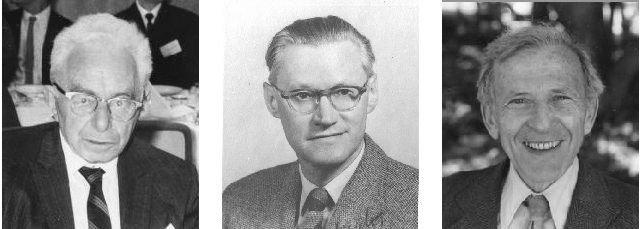
\includegraphics{Figures/f05Courant}}
\caption{Richard Courant (left), Kurt Friedrichs
(center), and  Hans Lewy (right) described the CFL
instability condition in 1928.}
\end{figure}


\labsection{Homework}
\begin{enumerate}
\prob Modify your leapfrog program to use $T = 1$ N and $\mu(x) = 0.1 +
{x\over L}$ so that the linear mass density of the guitar string
increases toward the right. (This makes the wave speed be a function of position, $c=c(x)$.)
Watch how the pulses propagate and explain qualitatively why they behave
as they do.
\end{enumerate}
\ifsolutions
\textit{Solution:}\\
\begin{codeexample}
\begin{VerbatimOut}{\listingFile}

class animatedWave():

    def __init__(self,a,b,N,tau,tMax,stabilityCheck = False,variableMu = False, T = 1, c = 2):
        from numpy import arange
        self.L = b        
        self.N = N
        self.tMax = tMax
        self.tau = tau
        self.dx = (b - a)/N
        self.x = arange(a - self.dx/2., b + self.dx,self.dx)

        if variableMu:
            from numpy import sqrt, array
            self.c = sqrt(T/array([self.mu(var) for var in self.x]))
        else: 
            self.c = c

        print stabilityCheck, 'here'
        from numpy import any
        if any(self.tau > self.dx/self.c) and stabilityCheck:
            print 'Beware: your algorithm will be unstable.'
            import sys
            sys.exit()


    def initializeWave(self):
        from numpy import exp,zeros
        # Gaussian initial displacement
        self.y = exp( -160/self.L**2 * (self.x - self.L/2.)**2 ) - exp( -160/self.L**2 * (0 - self.L/2.)**2 )
        # Zero initial velocity
        self.v = zeros(self.N+2)

    def mu(self,x):
        return 0.1 + x/self.L

    def animate(self):
        from numpy import zeros_like,copy
        from matplotlib import pyplot
        constant = self.c**2 * self.tau**2/(2 * self.dx**2)

        yOld = zeros_like(self.y)
        yOld[1:self.N + 1] = self.y[1:self.N+1] - self.v[1:self.N + 1] * self.tau + constant[1:self.N + 1] * (self.y[2:self.N + 2] - 2 * self.y[1:self.N + 1] + self.y[0:self.N])
        yOld[0] = -yOld[1]
        yOld[-1] = -yOld[-2]
        t = 0
        counter = 0
        while t < self.tMax:
            yNew = zeros_like(self.y)
            yNew[1:self.N + 1] = 2 * self.y[1:self.N+1] - yOld[1:self.N + 1] + constant[1:self.N + 1] * ( self.y[2:self.N + 2] - 2 * self.y[1:self.N + 1] + self.y[0:self.N])
            yNew[0] =  -yNew[1]
            yNew[-1] = - yNew[-2]

            if counter % 50 == 0:
                pyplot.plot(self.x,self.y,'r.-')
                pyplot.ylim(-1,1)
                pyplot.draw()
                pyplot.pause(.000001)
                pyplot.clf()


            yOld = copy(self.y)
            self.y = copy(yNew)


            t += self.tau
            counter += 1
a = 0
b = 1.
c = 2.
N = 200
tau = 0.001
tMax = 10

myWave = animatedWave(a,b,N,tau,tMax,stabilityCheck = True, variableMu = True)
myWave.initializeWave()
myWave.animate()
\end{VerbatimOut}
\end{codeexample}
\else
\noindent\rule{5 in}{0.01 in}
\fi





\chapter{The driven, damped wave equation}
\label{Lab:14}
Today we will continue solving the wave equation but we will add more
physics to the equation, making the simulation more realistic.  This
will come at the cost of algorithmic complexity.  Let's start by
adding some damping to the wave equation using a linear damping term, like this:
\begin{equation}\label{eq:WaveDamped}
    \frac{\partial^2 y}{\partial t^2}
    + \gamma \frac{\partial y}{\partial t}
    - c^2 \frac{\partial^2 y}{\partial x^2} = 0
\end{equation}

 with $c$ constant.  The staggered leapfrog method can be used to
solve Eq.~\eqref{eq:WaveDamped} also.  To do this, we use the
approximate first derivative formula
\begin{equation}
    \frac{\partial y}{\partial t} \approx \frac{y_j^{n+1} -
    y_j^{n-1}}{2 \tau}
\end{equation}


along with the second derivative formulas in
Eqs.~\eqref{eq:TimeDeriv} and \eqref{eq:SpaceDeriv} and find an
expression for the values one step in the future:
\begin{equation}\label{eq:stlfDamped}
    y_j^{n+1} = \frac{1}{2+\gamma \tau} \left (
    4 y_j^n - 2y_j^{n-1} + \gamma \tau y_j^{n-1}
    + \frac{2 c^2 \tau^2}{h^2} \left( y_{j+1}^n - 2 y_j^n + y_{j-1}^n
    \right) \right)
\end{equation}


\begin{enumerate}
\probtwo \label{P:14.1}
\begin{enumerate}

\subprob Derive Eq.~\eqref{eq:stlfDamped}.

\subprob Find a new formula for {\tt yold} using
Eqs.~\eqref{eq:leapfrogIV} and \eqref{eq:stlfDamped}, similar to what
we did to arrive at Eq.~\eqref{eq:yold}.\\
\marginfig[.2in]{Figures/f05p4}{The maximum amplitude
      of oscillation decays exponentially for the damped wave
      equation. (Problem~\ref{P:14.1d}) } Your answer should look like
    this:
\begin{equation}
  y_j^{-1} = -v_0(x_j) \frac{2 \tau(2+\gamma
    \tau) }{4 } + \left ( y_j^0 + \frac{c^2 \tau^2}{2h^2} \left( y_{j+1}^0 - 2 y_j^0 +
      y_{j-1}^0
    \right) \right) \\
\end{equation}

\ifsolutions
\textit{Solution:}
We will plug in this equation:
\begin{equation}
y_j^1 = \frac{1}{2+\gamma \tau} \left (
    4 y_j^0 - 2y_j^{-1} + \gamma \tau y_j^{-1}
    + \frac{2 c^2 \tau^2}{h^2} \left( y_{j+1}^0 - 2 y_j^0 + y_{j-1}^0
    \right) \right)
\end{equation}
into this one:
\begin{align}
    {y_j^1-y_j^{-1} \over 2 \tau} &= v_0(x_j)\\
\frac{1}{2 \tau(2+\gamma \tau)} \left (
    4 y_j^0 - 2y_j^{-1} + \gamma \tau y_j^{-1}
    + \frac{2 c^2 \tau^2}{h^2} \left( y_{j+1}^0 - 2 y_j^0 + y_{j-1}^0
    \right) \right) - {y_j^{-1} \over 2 \tau} = v_0(x_j)\\
\end{align}
collecting $y_j^{-1}$ terms:
\begin{align}
  \frac{-2 y_j^{-1} + \gamma \tau y_j^{-1}}{2 \tau(2+\gamma \tau)} -
  {y_j^{-1} \over 2 \tau} = v_0(x_j) - \frac{1}{2 \tau(2+\gamma \tau)}
  \left ( 4 y_j^0 + \frac{2 c^2 \tau^2}{h^2} \left( y_{j+1}^0 - 2
      y_j^0 + y_{j-1}^0
    \right) \right) \\
  \frac{-2 y_j^{-1} + \gamma \tau y_j^{-1} - (2 + \gamma \tau)
    y_j^{-1}}{2 \tau(2+\gamma \tau)} = v_0(x_j) - \frac{1}{2
    \tau(2+\gamma \tau)} \left ( 4 y_j^0 + \frac{2 c^2 \tau^2}{h^2}
    \left( y_{j+1}^0 - 2 y_j^0 + y_{j-1}^0
    \right) \right) \\
  y_j^{-1}\frac{-2 + \gamma \tau - (2 + \gamma \tau) }{2 \tau(2+\gamma
    \tau)} = v_0(x_j) - \frac{1}{2 \tau(2+\gamma \tau)} \left ( 4
    y_j^0 + \frac{2 c^2 \tau^2}{h^2} \left( y_{j+1}^0 - 2 y_j^0 +
      y_{j-1}^0
    \right) \right) \\
  y_j^{-1} = -v_0(x_j) \frac{2 \tau(2+\gamma
    \tau) }{4 } + \left ( y_j^0 + \frac{c^2 \tau^2}{2h^2} \left( y_{j+1}^0 - 2 y_j^0 +
      y_{j-1}^0
    \right) \right) \\
\end{align}

\fi
    \subprob \label{P:14.1b} Modify your staggered leapfrog code to
    include damping with $\gamma=0.2$. Then run your animation with
    the initial conditions in Problem~\ref{P:13.3c} and verify that
    the waves damp away.  You will need to run for about 25~s and you
    will want to use a big skip factor so that you don't have to wait
    forever for the run to finish.  

    \subprob \label{P:14.1d}Include some code to record the maximum value of $y(x)$
    over the entire grid as a function of time and then plot it as a
    function of time at the end of the run so that you can see the
    decay caused by $\gamma$. 

    \subprob The decay of a simple harmonic oscillator is exponential,
    with amplitude proportional to $e^{-\gamma t/2}$. Scale this time
    decay function properly and lay it over your maximum $y$ plot to
    see if it fits. Can you explain why the fit is as good as it is?
    (Hint: think about doing this problem via separation of
    variables.)  


\end{enumerate}
\ifsolutions
\textit{Solution:}\\
\begin{codeexample}
\begin{VerbatimOut}{\listingFile}

class animatedWave():

    def __init__(self,a,b,N,tau,tMax,gamma,stabilityCheck = False, c = 2):
        from numpy import arange
        self.L = b
        self.N = N
        self.tMax = tMax
        self.tau = tau
        self.gamma = gamma
        self.dx = (b - a)/N
        self.x = arange(a - self.dx/2., b + self.dx,self.dx)

        self.c = c

        print stabilityCheck, 'here'
        from numpy import any
        if any(self.tau > self.dx/self.c) and stabilityCheck:
            print 'Beware: your algorithm will be unstable.'
            import sys
            sys.exit()


    def initializeWave(self):
        from numpy import exp,zeros
        # Gaussian initial displacement
        self.v = 2 * exp( -160/self.L**2 * (self.x - self.L/2.)**2 )# - exp( -160/self.L**2 * (0 - self.L/2.)**2 )
        # Zero initial velocity
        self.y = zeros(self.N+2)


    def animate(self):
        from numpy import zeros_like,copy
        from matplotlib import pyplot
        constant = self.c**2 * self.tau**2/(2 * self.dx**2)
        constantTwo = 2. * self.tau * (2 + self.gamma * self.tau) 
        
        yOld = zeros_like(self.y)
        yOld[1:self.N + 1] = -self.v[1:self.N + 1] * constantTwo/4. +( self.y[1:self.N + 1] + constant *(self.y[2:self.N + 2]- 2 * self.y[1:self.N + 1] + self.y[0:self.N])) 
        yOld[0] = -yOld[1]
        yOld[-1] = -yOld[-2]
        t = 0
        counter = 0
        self.maxes = []
        while t < self.tMax:
            yNew = zeros_like(self.y)
            yNew[1:self.N + 1] = 1/(2 + self.gamma * self.tau) * (4 * self.y[1:self.N + 1] - 2 * yOld[1:self.N + 1] + self.gamma * self.tau * yOld[1:self.N + 1] + 4 * constant * (self.y[2:self.N + 2] - 2 * self.y[1: self.N + 1] + self.y[0:self.N]))
            yNew[0] =  -yNew[1]
            yNew[-1] = - yNew[-2]
            self.maxes.append(max(yNew))
            if counter % 50 == 0:
                pyplot.plot(self.x,self.y,'r.-')
                pyplot.ylim(-0.1,0.1)
                pyplot.draw()
                pyplot.pause(.000001)
                pyplot.clf()


            yOld = copy(self.y)
            self.y = copy(yNew)


            t += self.tau
            counter += 1
    def plotMaxes(self):
        from matplotlib import pyplot
        from numpy import linspace,exp
        t = linspace(0,self.tMax,len(self.maxes))
        pyplot.figure(2)
        pyplot.plot(t,self.maxes,'r.-')
        pyplot.plot(t,0.035 * exp(-self.gamma * t/2),'b-')
        pyplot.show()
a = 0
b = 1.
c = 2.
N = 200
tau = 0.001
gamma = 0.2
tMax = 25


myWave = animatedWave(a,b,N,tau,tMax,gamma,stabilityCheck = True)
myWave.initializeWave()
myWave.animate()
myWave.plotMaxes()
\end{VerbatimOut}
\end{codeexample}
\else
\noindent\rule{5 in}{0.01 in}
\fi

\end{enumerate}

\labsection{The damped and driven wave equation}

Finally, let's look at what happens when we add an oscillating
driving force to our string, so that the wave equation becomes
\begin{equation}\label{eq:WaveDampedDriven}
    \frac{\partial^2 y}{\partial t^2} + \gamma \frac{\partial
    y}{\partial t} - c^2 \frac{\partial^2 y}{\partial x^2} =
    \frac{f(x)}{\mu} \cos(\omega t)
\end{equation}
At the beginning of Lab~\ref{Lab:11} we discussed the
qualitative behavior of this system.  Recall that if we have a
string initially at rest and then we start to push and pull on
a string with an oscillating force/length of $f(x)$, we launch
waves down the string.  These waves reflect back and forth on
the string as the driving force continues to launch more waves.
The string motion is messy at first, but the damping in the
system causes the the transient waves from the initial launch
and subsequent reflections to eventually die away.  In the end,
we are left with a steady-state oscillation of the string at
the driving frequency $\omega$.

\marginfig[-2in]{Figures/f05p5}{Snapshots of the evolution a driven and
damped wave with $\omega=400$.  As the transient behavior dies
out, the oscillation goes to the resonant mode.  To make the
pictures more interesting, the string was not started from rest
in these plots. (In Problem~\ref{P:14.2} you start from rest for
easier coding.)}


\begin{enumerate}
  \probtwo \label{P:14.2} Model the motion of a damped, driven guitar
  string, clamped at both ends.  Since we are driving the oscillation with
  an external force, we can start with an undisplaced string with zero
  velocity.  This simplifies the initial conditions (just set $y=0$
  and $y_\mathrm{old}=0$ and enter the time-stepping loop). Use the
  following values for the string parameters: $T = 127$ N , $\mu =
  0.003$ kg/m, and $L = 1.2$ m and remember that $c=\sqrt{T/
    \mu}$. Use the same driving force as in Problem~\ref{P:11.1a}
\begin{equation}
\begin{array}{c}
 \\
f(x) \\
 \\
\end{array}
=
\left\{
\begin{array}{ll}
0.73 & {\rm if~~~} 0.8 \le x \le 1 \\
 & \\
0 & {\rm otherwise} \\
\end{array}
\right.
\end{equation}
and set the driving frequency at $\omega=400$.  
\begin{enumerate}
\subprob Derive an equation similar to Eq.~\eqref{eq:stlfDamped} but
that includes damping and driving as in
Eq.~\eqref{eq:WaveDampedDriven}.  Your answer should look like this:
\begin{multline}
    y_j^{n+1} = \frac{1}{2+\gamma \tau} \left (
    4 y_j^n - 2y_j^{n-1} + \gamma \tau y_j^{n-1}
    + \frac{2 c^2 \tau^2}{h^2} \left( y_{j+1}^n - 2 y_j^n + y_{j-1}^n
    \right) \right)\\ + \frac{f(x_j)}{\mu} \cos(\omega t) 
  \frac{2\tau^2}{(2 + \gamma \tau)}
\end{multline}

\subprob Modify your code from Problem~\ref{P:14.1} to use this new
algorithm.

\subprob Choose a damping constant $\gamma$ that is the proper size to
make the system settle down to steady state after 20 or 30 bounces of
the string. (You will have to think about the value of $\omega$ that
you are using and about your damping rate result from
problem~\ref{P:14.1} to decide which value of $\gamma$ to use to make
this happen.)

\subprob Run the model long enough that you can see the transients die
away and the string settle into the steady oscillation at the
driving frequency. You may find yourself looking at a flat-line
plot with no oscillation at all. If this happens look at the
vertical scale of your plot and remember that we are doing real
physics here. If your vertical scale goes from $-1$ to $1$, you
are expecting an oscillation amplitude of 1 meter on your
guitar string. Compare the steady state mode to the shape found
in Problem~\ref{P:11.1a} (see Fig.~\ref{Figures/f03p1a}).

Then run again with $\omega=1080$, which is close to a
resonance (see Fig.~\ref{Figures/f03p1b}), and again see the system
come into steady oscillation at the driving frequency.
\end{enumerate}
\end{enumerate}
\ifsolutions
\textit{Solution:}\\
\begin{codeexample}
\begin{VerbatimOut}{\listingFile}


class animatedWave():

    def __init__(self,a,b,N,tau,mu,T,omegaD,tMax,gamma,stabilityCheck = False, c = 2):
        from numpy import arange,sqrt
        self.L = b
        self.N = N
        self.tMax = tMax
        self.tau = tau
        self.mu = mu
        self.gamma = gamma
        self.T = T
        self.omegaD = omegaD
        self.dx = (b - a)/N
        self.x = arange(a - self.dx/2., b + self.dx,self.dx)

        self.c = sqrt(T/mu)

        if self.tau > self.dx/self.c and stabilityCheck:
            print 'Beware: your algorithm will be unstable.'
            import sys
            sys.exit()

    def f(self,x):
        import numpy
        if type(x) is numpy.ndarray:
            from numpy import array
            return array([self.f(var) for var in x])
        else:
            if 0.8 <= x <= 1.0:
                return 0.73
            else:
                return 0

    def initializeWave(self):
        from numpy import exp,zeros
        # Gaussian initial displacement
        self.v = 2 * exp( -160/self.L**2 * (self.x - self.L/2.)**2 ) - exp( -160/self.L**2 * (0 - self.L/2.)**2 )
        # Zero initial velocity
        self.y = zeros(self.N+2)


    def animate(self):
        from numpy import zeros_like,copy,cos
        from matplotlib import pyplot
        constant = self.c**2 * self.tau**2/(2 * self.dx**2)
        
        constantOne = 2. + self.gamma * self.tau
        constantTwo = 2. * self.c**2 * self.tau**2/self.dx**2

        yOld = zeros_like(self.y)
        yOld[1:self.N + 1] = -self.v[1:self.N + 1]* self.tau + 1./constantOne * (4 * self.y[1:self.N + 1] + constantTwo * (self.y[2:self.N + 2] - 2 * self.y[1:self.N + 1] + self.y[0:self.N])) + self.f(self.x[1:self.N + 1])/self.mu  * 2 * self.tau**2/constantOne
        yOld[0] = -yOld[1]
        yOld[-1] = -yOld[-2]
        t = 0
        counter = 0
        while t < self.tMax:
            yNew = zeros_like(self.y)
            yNew[1:self.N + 1] = 1/(2 + self.gamma * self.tau) * (4 * self.y[1:self.N + 1] - 2 * yOld[1:self.N + 1] + self.gamma * self.tau * yOld[1:self.N + 1]+ 4 * constant * (self.y[2:self.N + 2] - 2 * self.y[1: self.N + 1] + self.y[0:self.N])) + self.f(self.x[1:self.N + 1])/self.mu * cos(self.omegaD * t) * 2 * self.tau**2/(2 + self.gamma * self.tau)
            yNew[0] =  -yNew[1]
            yNew[-1] = - yNew[-2]
            if counter % 50 == 0:
                pyplot.plot(self.x,self.y,'r.-')
                pyplot.ylim(-0.005,0.005)
                pyplot.draw()
                pyplot.pause(.000001)
                pyplot.clf()


            yOld = copy(self.y)
            self.y = copy(yNew)


            t += self.tau
            counter += 1
a = 0
b = 1.2
N = 200
tau = 0.00001
gamma = 60
tMax = 25.
mu = .003
T = 127.
omegaD = 1080.


myWave = animatedWave(a,b,N,tau,mu,T,omegaD,tMax,gamma,stabilityCheck = True)
myWave.initializeWave()
myWave.animate()

\end{VerbatimOut}
\end{codeexample}
\else
\noindent\rule{5 in}{0.01 in}
\fi

\labsection{Homework}

\begin{enumerate}
  \prob Use the staggered leapfrog algorithm to study how pulses
  propagate along a hanging chain. 
The wave equation for transverse waves on a chain with a varying
tension ($T(x)$), constant linear mass density ($\mu$), including
damping and an external driving force is given by:
\begin{equation}\label{eq:WaveDampedDrivenVariableTension}
    \frac{\partial^2 y}{\partial t^2} + \gamma \frac{\partial
    y}{\partial t} - \frac{1}{\mu}\frac{\partial }{\partial x}\left(T(x)
    \frac{\partial y }{\partial x} \right) =
    \frac{f(x)}{\mu} \cos(\omega t)
\end{equation}
Here are some steps that you can follow to help you accomplish this:
\begin{enumerate}
\subprob \label{P:14.3}Recall that $T(x) = \mu g x$ for a hanging chain.  Insert
this into equation \eqref{eq:WaveDampedDrivenVariableTension} and
evaluate the third term on the left.\\
\ifsolutions
\textit{Solution:}
\begin{align}
\frac{\partial ^2y}{\partial t^2} - g \frac{\partial}{\partial
  x} \left( x \frac{\partial y}{\partial x}\right) + \gamma
\frac{\partial y}{\partial t} &= \frac{f(x)}{\mu} \cos(\omega t)\\
\frac{\partial ^2y}{\partial t^2} - g \left( \frac{\partial
    y}{\partial x} + x \frac{\partial^2 y}{\partial x^2}\right) + \gamma
\frac{\partial y}{\partial t} &= \frac{f(x)}{\mu} \cos(\omega t)\\
\end{align}
\fi
\subprob Now discretize the equation and rearrange to solve for
$y_j^{n+1}$ just as we did in equation \eqref{leapfrog} (Don't lose
track of your superscripts and subsripts).  Your answer should look
like this:
\begin{multline}
  y_j^{n+1} = \frac{2\tau^2}{\left( 2 + \gamma \tau\right)} \frac{f(x_j)}{\mu}
  \cos (\omega t_j) + \frac{2\tau^2 g }{\left( 2 + \gamma
      \tau\right)} \left( \frac{y_{j+1}^n - y_{j-1}^n}{2 dx}\right)\\ +
  \frac{2\tau^2 g }{\left( 2 + \gamma \tau\right)} x_j\left(
    \frac{y_{j+1}^n - 2 y_j^n + y_{j-1}^n}{dx^2}\right) +
  \frac{2\tau^2}{\left( 2 + \gamma \tau\right)}\left(\frac{ 2
      y_j^n - y_j^{n-1}}{\tau^2}\right) +
  \frac{ 2\tau^2\gamma}{\left( 2 + \gamma \tau\right)} \left(
    \frac{ y_j^{n-1}}{2 \tau}\right) 
\end{multline}
\ifsolutions
\textit{Solution:}
\begin{multline}
  \left(\frac{y_j^{n+1} - 2 y_j^n + y_j^{n-1}}{\tau^2}\right) - g
  \left( \frac{y_{j+1}^n - y_{j-1}^n}{2 dx}\right) - g x_j\left(
    \frac{y_{j+1}^n - 2 y_j^n + y_{j-1}^n}{dx^2}\right)\\ + \gamma
  \left( \frac{y_j^{n+1} - y_j^{n-1}}{2 \tau}\right) = \frac{f(x_j)}{\mu} \cos
  (\omega t_j)
\end{multline}
\begin{multline}
\left(\frac{y_j^{n+1} - 2 y_j^n + y_j^{n-1}}{\tau^2}\right) +
  \gamma \left( \frac{y_j^{n+1} - y_j^{n-1}}{2 \tau}\right) = \frac{f(x_j)}{\mu}
  \cos (\omega t_j)\\ + g \left( \frac{y_{j+1}^n - y_{j-1}^n}{2
      dx}\right) + g x_j\left( \frac{y_{j+1}^n  - 2 y_j^n +
      y_{j-1}^n}{dx^2}\right) 
\end{multline}
\begin{multline}
  \frac{y_j^{n+1}}{\tau^2} + \frac{\gamma y_j^{n+1}}{2 \tau} -
  \left(\frac{ 2 y_j^n - y_j^{n-1}}{\tau^2}\right) - \gamma \left(
    \frac{ y_j^{n-1}}{2 \tau}\right) = \frac{f(x_j)}{\mu} \cos (\omega t_j)\\ + g
  \left( \frac{y_{j+1}^n - y_{j-1}^n}{2 dx}\right) + g
  x_j\left( \frac{y_{j+1}^n - 2 y_j^n +
      y_{j-1}^n}{dx^2}\right) 
\end{multline}
\begin{multline}
  \frac{ y_j^{n+1}}{\tau^2} + \frac{\gamma y_j^{n+1}}{2 \tau} =
  \frac{f(x_j)}{\mu} \cos (\omega t_j) + g \left( \frac{y_{j+1}^n -
      y_{j-1}^n}{2 dx}\right) + g x_j\left( \frac{y_{j+1}^n - 2
      y_j^n + y_{j-1}^n}{dx^2}\right)\\ + \left(\frac{ 2 y_j^n -
      y_j^{n-1}}{\tau^2}\right) +
  \gamma \left( \frac{ y_j^{n-1}}{2 \tau}\right) 
\end{multline}
\begin{multline}
  \frac{2 y_j^{n+1} + \gamma \tau y_j^{n+1}}{2\tau^2} = \frac{f(x_j)}{\mu} \cos
  (\omega t_j) + g \left( \frac{y_{j+1}^n - y_{j-1}^n}{2
      dx}\right) + g x_j\left( \frac{y_{j+1}^n - 2 y_j^n +
      y_{j-1}^n}{dx^2}\right)\\ + \left(\frac{ 2 y_j^n -
      y_j^{n-1}}{\tau^2}\right) +
  \gamma \left( \frac{ y_j^{n-1}}{2 \tau}\right) 
\end{multline}
\begin{multline}
  y_j^{n+1}\left( 2 + \gamma \tau\right) = 2\tau^2 \frac{f(x_j)}{\mu} \cos
  (\omega t_j) + 2\tau^2 g \left( \frac{y_{j+1}^n - y_{j-1}^n}{2
      dx}\right)\\ + 2\tau^2 g x_j\left( \frac{y_{j+1}^n - 2 y_j^n +
      y_{j-1}^n}{dx^2}\right) + 2\tau^2\left(\frac{ 2 y_j^n -
      y_j^{n-1}}{\tau^2}\right) +
  2\tau^2\gamma \left( \frac{ y_j^{n-1}}{2 \tau}\right) 
\end{multline}
\begin{multline}
  y_j^{n+1} = \frac{2\tau^2}{\left( 2 + \gamma \tau\right)} \frac{f(x_j)}{\mu}
  \cos (\omega t_j) + \frac{2\tau^2 g }{\left( 2 + \gamma
      \tau\right)} \left( \frac{y_{j+1}^n - y_{j-1}^n}{2 dx}\right)\\ +
  \frac{2\tau^2 g }{\left( 2 + \gamma \tau\right)} x_j\left(
    \frac{y_{j+1}^n - 2 y_j^n + y_{j-1}^n}{dx^2}\right) +
  \frac{2\tau^2}{\left( 2 + \gamma \tau\right)}\left(\frac{ 2
      y_j^n - y_j^{n-1}}{\tau^2}\right) +
  \frac{ 2\tau^2\gamma}{\left( 2 + \gamma \tau\right)} \left(
    \frac{ y_j^{n-1}}{2 \tau}\right) 
\end{multline}
% \restoregeometry
\fi \subprob The initial conditions are easy enough to include (we'll
just set the initial displacement and velocity to 0 and let the
driving force create the disturbance) but we'll have to think a bit
harder about the boundary conditions.  At $x=L$, the rope is fixed to
the ceiling so $y(L,t) = 0$.  The harder one is at $x = 0$ where the
chain is allowed to flap around as it pleases.  To get the boundary
condition at $x = 0$ start with the equation that you arrived at in
part (a) and evaluate it at $x=0$.  Then discretize this equation and
solve it for $ y_0^{n+1}$ to get the desired boundary condition. Your answer should look
like this:
\begin{multline}
  y_0^{n+1}   = \left(\frac{4 \tau^2 }{2 + \gamma \tau}\right)\frac{f(x_j)}{\mu} \cos
  (\omega t_j) - \left(\frac{2 - \gamma \tau }{2 + \gamma
      \tau}\right)\left(  y_1^{n - 1} + y_0^{n - 1}\right) \\ +
  \left(\frac{4 }{2 + \gamma \tau}\right)\left(y_1^n + y_0^n\right) +
  \left(\frac{4 \tau^2g }{2 + \gamma \tau}\right)\left( \frac{y_1^n -
      y_0^n}{ dx}\right) - y_1^{n + 1}
\end{multline}

\ifsolutions
\textit{Solution:}
%\newgeometry{left = -40 cm,right = 0 cm}
When $x = 0$, the discrete version of the differential equation is
\begin{multline}
  \left(\frac{y_j^{n+1} - 2 y_j^n + y_j^{n-1}}{\tau^2}\right) - g
  \left( \frac{y_{j+1}^n - y_{j-1}^n}{2 dx}\right) \\ + \gamma
  \left( \frac{y_j^{n+1} - y_j^{n-1}}{2 \tau}\right) = \frac{f(x_j)}{\mu} \cos
  (\omega t_j)
\end{multline}
Let's collect like terms:
\begin{multline}
  y_j^{n+1} \left( {1\over \tau^2} + {\gamma \over 2 \tau}\right)  +
  y_j^{n-1}\left( {1\over \tau^2} - {\gamma \over 2 \tau}\right) - {2\over
      \tau^2} y_j^n - g \left( \frac{y_{j+1}^n - y_{j-1}^n}{2 dx}\right)\\ = \frac{f(x_j)}{\mu} \cos
  (\omega t_j)
\end{multline}
Now we need to evaluate this equation at $x = 0$.  The spatial
derivative term (4th term on l.h.s) is easily evaluated at this point:
\begin{multline}
  y_j^{n+1} \left( {1\over \tau^2} + {\gamma \over 2 \tau}\right)  +
  y_j^{n-1}\left( {1\over \tau^2} - {\gamma \over 2 \tau}\right) - {2\over
      \tau^2} y_j^n - g \left( \frac{y_1^n - y_0^n}{ dx}\right)\\ = \frac{f(x_j)}{\mu} \cos
  (\omega t_j)
\end{multline}
but for the other terms we can't just set $j = 0$ because that's not
the end point of our domain.  Instead we need to set 
\begin{multline}
\left(  \frac{y_1^{n + 1} + y_0^{n+1}}{2}\right) \left( {1\over \tau^2} + {\gamma \over 2 \tau}\right)  +
  \left(\frac{y_1^{n - 1} + y_0^{n-1}}{2}\right)\left( {1\over \tau^2} - {\gamma \over 2 \tau}\right) - {2\over
      \tau^2} \left(\frac{y_1^n + y_0^n}{2}\right) - g \left( \frac{y_1^n - y_0^n}{ dx}\right)\\ = \frac{f(x_j)}{\mu} \cos
  (\omega t_j)
\end{multline}
Now we need to solve for $y_0^{n+1}$:
\begin{multline}
  \left(  \frac{y_1^{n + 1} + y_0^{n+1}}{2}\right) \left( {1\over \tau^2} + {\gamma \over 2 \tau}\right)  \\ = \frac{f(x_j)}{\mu} \cos
  (\omega t_j) - \left(  \frac{y_1^{n - 1} + y_0^{n - 1}}{2}\right)\left( {1\over \tau^2} - {\gamma \over 2 \tau}\right) + {2\over
      \tau^2} \left(  \frac{y_1^n + y_0^n}{2}\right) + g \left( \frac{y_1^n - y_0^n}{ dx}\right)
\end{multline}
\begin{multline}
  \left(  \frac{y_1^{n + 1} + y_0^{n+1}}{2}\right) \left(\frac{2 + \gamma \tau}{2 \tau^2}\right)   = \frac{f(x_j)}{\mu} \cos
  (\omega t_j) - \left(  \frac{y_1^{n - 1} + y_0^{n - 1}}{2}\right) \left(\frac{2 - \gamma \tau}{2 \tau^2}\right)\\ + \left(\frac{y_1^n + y_0^n}{\tau^2}\right) + g \left( \frac{y_1^n - y_0^n}{ dx}\right)
\end{multline}
\begin{multline}
  \left(  y_1^{n + 1} + y_0^{n+1}\right)   = \left(\frac{4 \tau^2 }{2 + \gamma \tau}\right)\frac{f(x_j)}{\mu} \cos
  (\omega t_j) - \left(\frac{4 \tau^2 }{2 + \gamma \tau}\right)\left(
    \frac{y_1^{n - 1} + y_0^{n - 1}}{2}\right) \left(\frac{2 - \gamma \tau}{2 \tau^2}\right)\\ + \left(\frac{4 \tau^2 }{2 + \gamma \tau}\right)\left(\frac{y_1^n + y_0^n}{\tau^2}\right) + \left(\frac{4 \tau^2 }{2 + \gamma \tau}\right) g \left( \frac{y_1^n - y_0^n}{ dx}\right)
\end{multline}
\begin{multline}
  \left(  y_1^{n + 1} + y_0^{n+1}\right)   = \left(\frac{4 \tau^2 }{2 + \gamma \tau}\right)\frac{f(x_j)}{\mu} \cos
  (\omega t_j) - \left(\frac{2 - \gamma \tau }{2 + \gamma
      \tau}\right)\left(  y_1^{n - 1} + y_0^{n - 1}\right) \\ + \left(\frac{4 }{2 + \gamma \tau}\right)\left(y_1^n + y_0^n\right) + \left(\frac{4 \tau^2g }{2 + \gamma \tau}\right)\left( \frac{y_1^n - y_0^n}{ dx}\right)
\end{multline}
\begin{multline}
  y_0^{n+1}   = \left(\frac{4 \tau^2 }{2 + \gamma \tau}\right)\frac{f(x_j)}{\mu} \cos
  (\omega t_j) - \left(\frac{2 - \gamma \tau }{2 + \gamma
      \tau}\right)\left(  y_1^{n - 1} + y_0^{n - 1}\right) \\ +
  \left(\frac{4 }{2 + \gamma \tau}\right)\left(y_1^n + y_0^n\right) +
  \left(\frac{4 \tau^2g }{2 + \gamma \tau}\right)\left( \frac{y_1^n -
      y_0^n}{ dx}\right) - y_1^{n + 1}
\end{multline}

\fi

\subprob With the two initial condition, the two boundary conditions
and the differential equation all discretized, we are ready to code.
Code up the staggered leapfrog for this situation.  Let the animation
run for several periods of the motion to verify that it is behaving in
a way that you would expect.
\end{enumerate}
\end{enumerate}
\ifsolutions
\textit{Solution:}\\
\begin{codeexample}
\begin{VerbatimOut}{\listingFile}
class animatedWave():

    def __init__(self,a,L,N,tau,tMax,gamma, mu,stabilityCheck = False):
        from numpy import arange
        self.L = L
        #self.c = c
        self.N = N
        self.tMax = tMax
        self.tau = tau
        self.gamma = gamma
        self.mu = mu
        self.g = 9.8
        self.omegaD = 15.
        self.dx = (b - a)/N

        
        self.x = arange(a - self.dx/2, b + self.dx,self.dx)

        cTop = self.mu * self.L * self.g
        if self.tau > self.dx/cTop and stabilityCheck:
            print "Beware: You are numerically unstable"
            import sys
            sys.exit()

    def f(self,x):
        import numpy
        if type(x) is numpy.ndarray:
            from numpy import array
            return array([self.f(var) for var in x])
        else:
            if   0.45 < x < 0.5:
                return 1.73
            else:
                return 0
    def initializeWave(self):
        from numpy import exp,zeros

        self.v = zeros(self.N + 2)#exp(-160/self.L**2 * (self.x - self.L/2.)**2) - exp(-160/self.L**2 * (0 - self.L/2.)**2)
        self.y = zeros(self.N + 2)

    def animate(self):
        from numpy import zeros_like,copy,cos
        #        constant = self.c**2 * self.tau**2/(2 * self.dx**2)

        constant = 2 * self.tau**2/(2 + self.gamma * self.tau)

        constantFive = 4 * self.tau**2/(2 + self.gamma * self.tau)
        yOld = zeros_like(self.y)

        t = 0
        counter = 0
        while t < self.tMax:
            yNew = zeros_like(self.y)
            yNew[1:self.N+1] = constant * self.f(self.x[1:self.N + 1])/self.mu * cos(self.omegaD * t) + constant * self.g * (self.y[2:self.N + 2] - self.y[0:self.N])/(2 * self.dx) + constant * self.g * self.x[1:self.N + 1] * (self.y[2:self.N + 2] - 2 * self.y[1:self.N + 1] + self.y[0:self.N])/self.dx**2 + constant * (2 * self.y[1:self.N + 1] - yOld[1:self.N + 1])/self.tau**2 + constant * self.gamma *yOld[1:self.N +1]/(2 * self.tau)
#            print 'first term', - constantFive * (2 - self.gamma * self.tau)/(4 * self.tau**2) *(yOld[1] + yOld[0])
#            print 'second term',  constantFive /self.tau**2 *(self.y[1] + self.y[0])
#            print 'third term', - yNew[1]
#            print 'fourth term', self.g /self.dx * constantFive *(self.y[1] - self.y[0])
#            print 'fifth term',   self.f(0)/self.mu * constantFive * cos(self.omegaD * t)
            
            yNew[0] =    - constantFive * (2 - self.gamma * self.tau)/(4 * self.tau**2) *(yOld[1] + yOld[0])  +   constantFive /self.tau**2 *(self.y[1] + self.y[0]) - yNew[1] + self.g /self.dx * constantFive *(self.y[1] - self.y[0]) +  self.f(0)/self.mu * constantFive * cos(self.omegaD * t)
            #            print yNew[0], 't = ', t
            #input('press a key')
            yNew[-1] = -yNew[-2]

            if counter %100 == 0:
                from numpy import pi
                from matplotlib import pyplot
                pyplot.plot(self.y,self.x,'r.-')
                pyplot.xlim(-1.25,1.25)
                pyplot.ylim(-0.05,1.25)
                pyplot.title("T = " + str(2 * pi/self.omegaD)+  ' s\n time:'+ str(t))
                pyplot.draw()
                pyplot.pause(.001)
                pyplot.clf()



            yOld = copy(self.y)
            self.y = copy(yNew)
            t += self.tau
            counter += 1

a = 0
b = 1.
N = 200
tau = .0001
gamma = 20
mu = 0.003
tMax = 10
myWave = animatedWave(a,b,N,tau,tMax,gamma,mu,stabilityCheck=True)
myWave.initializeWave()
myWave.animate()
\end{VerbatimOut}
\end{codeexample}
\else
\noindent\rule{5 in}{0.01 in}
\fi

%Challenge Problem.
%Use the staggered leapfrog algorithm to study how pulses propagate along
%a hanging chain.
%You will have to work at making the boundary condition at the bottom of
%the chain work properly.
%Derive this boundary condition from the wave equation on the chain by looking
%at the wave equation at $x=0$.

\chapter{The 2-D Wave Equation With Staggered Leapfrog}
\label{Lab:15}
 \index{Wave equation!two dimensions}
 \index{Two-dimensional wave equation}

\labsection{Two dimensional grids}
\index{Two-dimensional grids}
\index{Grids!two-dimensional}

\marginfig{Figures/f06Grids2d}{Two types of 2-D grids.}

In this lab we will do problems in two spatial dimensions, $x$ and
$y$, so we need to spend a little time thinking about how to
represent 2-D grids.  For a simple rectangular grid where all of the
cells are the same size, 2-D grids are pretty straightforward. We
just divide the $x$-dimension into equally sized regions and the
$y$-dimension into equally sized regions, and the two one dimensional
grids intersect to create rectangular cells.  Then we put grid points
either at the corners of the cells (cell-edge) or at the centers of
the cells (cell-centered).  On a cell-center grid we'll usually want
ghost point outside the region of interest so we can get the boundary
conditions right.

\begin{enumerate}
\probtwo \label{P:15.1} Numpy has a nice way of representing
    rectangular two-dimensional grids using the {\tt meshdgrid}
    command.\index{meshdgrid} Let's take a minute to
    learn how to make surface plots using this command.
    Consider a 2-d rectangle defined by $x \in [a,b]$ and $y
    \in [c,d]$. To create a 30-point cell-edge grid in $x$ and
    a 50-point cell-edge grid in $y$ with $a=0$, $b=2$, $c=-1$,
    $d=3$, we use the following code:
\begin{Verbatim}
from numpy import linspace,meshgrid
a = 0
b = 2
Nx = 30
x,dx = linspace(a,b,Nx,retstep = True)

c = 1
d = 3
Ny = 50
y,dy = linspace(c,d,Ny,retstep = True)


X,Y=meshgrid(x,y);
\end{Verbatim}
    \begin{enumerate}

\subprob Put the code fragment above in a script and run
    it to create the 2-D grid. Examine the contents of {\tt
    X} and {\tt Y} thoroughly enough that you can explain
    what the {\tt meshgrid} command does.  See the first
    section of chapter 9 in \emph{Introduction to Python}
    for help understanding the indexing.


\subprob Using this 2-D grid, evaluate the following function
    of $x$ and $y$:
    \begin{equation}
        f(x,y) = e^{(-(x^2+y^2))} \cos{(5 \sqrt{x^2+y^2})}
    \end{equation}

    Use Python's \texttt{plot\_surface} or \texttt{plot\_wireframe}
    command to make a surface plot of this function. \marginfig{Figures/f06p1}{Plot
      from Problem~\ref{P:15.1}} Then properly label the $x$ and $y$
    axes with the symbols $x$ and $y$, to get a plot like
    Fig.~\ref{Figures/f06p1}.
\end{enumerate}
\end{enumerate}
\ifsolutions
\textit{Solution:}\\
\begin{codeexample}
\begin{VerbatimOut}{\listingFile}
from numpy import linspace, meshgrid,exp,sqrt,cos
from matplotlib import pyplot
from mpl_toolkits.mplot3d import Axes3D

a = 0
b = 2
c = -3
d = 3
Nx = 30
Ny = 50
x,dx = linspace(a,b,Nx,retstep = True)
y,dy = linspace(c,d,Ny,retstep = True)

X,Y = meshgrid(x,y)

z = exp(-(X**2 + Y**2)) * cos(5 * sqrt(X**2 + Y**2))
fig = pyplot.figure()
ax = fig.gca(projection='3d')
ax.plot_surface(X,Y,z)
pyplot.show()
\end{VerbatimOut}
\end{codeexample}
\else
\noindent\rule{5 in}{0.01 in}
\fi


\labsection{The two-dimensional wave equation}


The wave equation for transverse waves on a rubber sheet is
\footnote{N.\ Asmar, {\it Partial Differential Equations and Boundary
Value Problems} (Prentice Hall, New Jersey, 2000), p. 129-134.}
\begin{equation}\label{eq:2dwave}
    \mu {\partial^2 z \over \partial t^2}= \sigma \left(
    {\partial^2 z \over \partial x^2} +
    {\partial^2 z \over \partial y^2} \right)
\end{equation}
In this equation $\mu$ is the surface mass density of the sheet, with
units of mass/area. The quantity $\sigma$ is the surface tension,
which has rather odd units. By inspecting the equation above you can
find that $\sigma$ has units of force/length, which doesn't seem
right for a surface. But it is, in fact, correct as you can see by
performing the following thought experiment. Cut a slit of length $L$
in the rubber sheet and think about how much force you have to exert
to pull the lips of this slit together. Now imagine doubling $L$;
doesn't it seem that you should have to pull twice as hard to close
the slit? Well, if it doesn't, it should; the formula for this
closing force is given by $\sigma L$, which defines the meaning of
$\sigma$.

We can solve the two-dimensional wave equation using the same
staggered leapfrog techniques that we used for the one-dimensional
case, except now we need to use a two dimensional grid to represent
$z(x,y,t)$.  We'll use the notation $z_{j,k}^n = z(x_j,y_k,t_n)$ to
represent the function values.  With this notation, the derivatives
can be approximated as
\begin{equation}
    \frac{\partial^2 z}{\partial t^2} \approx
    \frac{z_{j,k}^{n+1} - 2 z_{j,k}^{n} + z_{j,k}^{n-1}}{\tau^2}
\end{equation}
\begin{equation}
    \frac{\partial^2 z}{\partial x^2} \approx
    \frac{z_{j+1,k}^{n} - 2 z_{j,k}^{n} + z_{j-1,k}^{n}}{h_x^2}
\end{equation}
\begin{equation}
    \frac{\partial^2 z}{\partial y^2} \approx
    \frac{z_{j,k+1}^{n} - 2 z_{j,k}^{n} + z_{j,k-1}^{n}}{h_y^2}
\end{equation}
where $h_x$ and $h_y$ are the grid spacings in the $x$ and $y$
dimensions.  We insert these three equations into
Eq.~\eqref{eq:2dwave} to get an expression that we can solve for $z$
at the next time (i.e. $z_{j,k}^{n+1}$).  Then we use this expression
along with the discrete version of the initial velocity condition
\begin{equation}\label{eq:tDeriv}
    v_0(x_j,y_k) \approx \frac{z_{j,k}^{n+1} - z_{j,k}^{n-1}}{2 \tau}
\end{equation}
to find an expression for the initial value of $z_{j,k}^{n-1}$
(i.e. {\tt zold}) so we can get things started.

\marginfig[-1in]{Figures/f06p2}{A wave on a rubber sheet with fixed
edges.}

\begin{enumerate}
\probtwo \label{P:15.2}
\begin{enumerate}
\subprob Derive the staggered leapfrog algorithm for the case
    of square cells with $h_x = h_y = h$. You should arrive at the
    following equation:
\begin{equation}
z_{j,k}^{n+1} = 2 z_{j,k}^n - z_{j,k}^{n-1} + \frac{\sigma \tau^2}{\mu
h^2} \left( z_{j+1,k}^n - 4 z_{j,k}^n + z_{j-1,k}^n + z_{j,k+1}^n + z_{j,k-1}^n\right)
\end{equation}

\subprob Notice that to find the state of the wave at a future moment,
you are going to need the state of the wave at two previous moments.
Use equation \eqref{eq:tDeriv} together with your result from part (a)
to find an expression for \texttt{zold}. You've done this several
times before so this should not feel too foreign to you. You should
find that:
\begin{equation}
z_{j,k}^{-1} = z_{j,k}^0 - v_{j,k}^0 \tau + \frac{\sigma \tau^2}{2\mu
h^2} \left( z_{j+1,k}^0 - 4 z_{j,k}^0 + z_{j-1,k}^0 + z_{j,k+1}^0 + z_{j,k-1}^0\right)
\end{equation}

\subprob Write a Python script that animates the solution of the two
dimensional wave equation on a square region that is
$[-5,5]\times[-5,5]$ and that has fixed edges. Use a
\textbf{cell-edge} square grid with the edge-values pinned to
zero. Choose $\sigma=2$~N/m and $\mu=0.3$~kg/m$^2$ and use a
displacement initial condition that is a Gaussian pulse with zero
velocity
    \begin{equation}
        z(x,y,0) = e^{-5(x^2+y^2)}
        \label{sheetpulse}
    \end{equation}
    This initial condition doesn't strictly satisfy the
    boundary conditions, so you should pin the edges to zero.
%Define index variables {\tt j} and {\tt k} like this
%\begin{Verbatim}
%    j = 2:Nx+1;
%    k = 2:Ny+1;
%\end{Verbatim}
%so you can write the code cleanly like this:
%\begin{Verbatim}
%znew(j,k)= ...  z(j-1,k) + z(j+1,k) ...
%\end{Verbatim}

    Run the simulation long enough that you see the effect of
    repeated reflections from the edges.  

\subprob You will find that this two-dimensional problem has
    a Courant condition similar to the one-dimensional case,
    but with a factor out front:
    \begin{equation}
        \tau < f {h \over c}
    \end{equation}
    where $c = \sqrt{\sigma \over \mu}$.  Determine the value of the
    constant $f$ by numerical experimentation. (Try various values of
    $\tau$ and discover where the boundary is between numerical
    stability and instability.)

\subprob Also watch what happens at the center of the sheet
    by making a plot of $z(0,0,t)$ there. In one dimension
    the pulse propagates away from its initial position
    making that point quickly come to rest with $z=0$. This
    also happens for the three-dimensional wave equation. But
    something completely different happens in two (and
    higher) even dimensions; you should be able to see it in
    your plot by looking at the behavior of $z(0,0,t)$ before
    the first reflection comes back.


\subprob Finally, change the initial conditions so that the
    sheet is initially flat but with the initial velocity
    given by the Gaussian pulse of Eq.~(\ref{sheetpulse}). In
    one dimension when you pulse the system like this the
    string at the point of application of the pulse moves up
    and stays up until the reflection comes back from the
    ends of the system. Does the same thing happen in
    the middle of the sheet when you apply this initial
    velocity pulse? Answer this question by looking at your
    plot of $z(0,0,t)$. You should find that the
    two-dimensional wave equation behaves very differently
    from the one-dimensional wave equation.
\end{enumerate}
\end{enumerate}
\ifsolutions
\textit{Solution:}\\
\begin{codeexample}
\begin{VerbatimOut}{\listingFile}




class TwoDWave():

    def __init__(self,a,b,c,d,N,mu,sigma,tau,tMax):
        from numpy import linspace,meshgrid,sqrt
        self.tau = tau
        self.mu = mu
        self.sigma = sigma
        self.N = N
        self.tMax = tMax
        self.c = sqrt(sigma/mu)
        x,self.dx = linspace(a,b,N,retstep = True)
        y,self.dy = linspace(c,d,N,retstep = True)
        self.X,self.Y = meshgrid(x,y)
        print(self.dx)
        print( "Courant condition: ", self.dx/self.c/sqrt(2))
        if self.tau > 1/( sqrt(2)) *  self.dx/self.c:
            print(self.tau)
            print(1/( sqrt(2)) *  self.dx/self.c)
            print("Instability headed your way!")
            import sys
            sys.exit()

    def initializeWave(self):
        from numpy import zeros_like,exp
        
        self.z = exp(-5 *(self.X**2 + self.Y**2))
        self.v = zeros_like(self.z)
        self.z[0] = 0
        self.z[-1] = 0
        self.z[:,0] = 0
        self.z[:,-1] = 0
    def animate(self,movie=True):
        from numpy import zeros_like,copy
        from matplotlib import pyplot,cm
        from mpl_toolkits.mplot3d import Axes3D
        
        constant = self.sigma * self.tau**2 /(self.mu * self.dx**2)
        #        constant = self.c**2 * self.tau**2 /self.dx**2
        zOld = zeros_like(self.z)
        zOld[1:self.N - 1,1:self.N - 1] = - self.tau * self.v[1:self.N - 1,1:self.N - 1] + self.z[1:self.N -1, 1:self.N -1] + constant/2 * (self.z[2:self.N,1:self.N - 1] - 2 * self.z[1:self.N - 1,1:self.N - 1] + self.z[0:self.N - 2,1:self.N - 1] + self.z[1:self.N - 1,2:self.N] - 2 * self.z[1:self.N - 1,1:self.N - 1] + self.z[1:self.N - 1,0:self.N - 2])
        zOld[0] = 0
        zOld[-1] = 0
        zOld[:,0] = 0
        zOld[0,:] = 0

        counter = 0
        t = 0
        fig = pyplot.figure()
        self.singlePoint = []
        while t < self.tMax:
            zNew = zeros_like(self.z)
            zNew[1:self.N - 1,1:self.N - 1] = 2 * self.z[1:self.N - 1,1:self.N - 1] - zOld[1:self.N - 1, 1: self.N - 1] + constant * (self.z[2:self.N,1:self.N - 1] - 2 * self.z[1:self.N - 1,1:self.N - 1] + self.z[0:self.N - 2,1:self.N - 1] + self.z[1:self.N - 1,2:self.N] - 2 * self.z[1:self.N - 1,1:self.N - 1] + self.z[1:self.N - 1,0:self.N - 2])
            zNew[0] = 0
            zNew[-1] = 0
            zNew[:,0] = 0
            zNew[0,:] = 0
            self.singlePoint.append(self.z[int(self.N/2),int(self.N/2)])
            if counter %50 == 0 and movie:
                ax = fig.gca(projection='3d')
                ax.plot_surface(self.X,self.Y,self.z,cmap=cm.coolwarm)
                ax.set_zlim(-.5,.5)
                pyplot.draw()
                pyplot.pause(.0001)
                pyplot.clf()
                
            zOld = copy(self.z)
            self.z = copy(zNew)
            t += self.tau
            counter += 1
    def plotSinglePoint(self):

        from matplotlib import pyplot
        from numpy import linspace
        pyplot.plot(linspace(0,self.tMax,len(self.singlePoint)),self.singlePoint)
        pyplot.show()

a = -5
b = 5
c = -5
d = 5
N = 100
mu = 0.3
sigma = 2
tau = .005
tMax = 50
my2Dwave = TwoDWave(a,b,c,d,N,mu,sigma,tau,tMax)
my2Dwave.initializeWave()
my2Dwave.animate()
my2Dwave.plotSinglePoint()

#from numpy import linspace, meshgrid,exp,sqrt,cos
#from matplotlib import pyplot
#from mpl_toolkits.mplot3d import Axes3D
\end{VerbatimOut}
\end{codeexample}
\else
\noindent\rule{5 in}{0.01 in}
\fi

\labsection{Homework}
\begin{enumerate}
\prob Consider the same square membrane from problem \ref{P:15.2} but
instead of a constant mass density, let's use the following function:
\begin{equation}
\mu(x,y) = 2.3 - 0.2 x - 0.2 y
\end{equation}
Modify your code to model the motion of this membrane.  Think about
how you will calculate your Courant condition.
\end{enumerate}
\ifsolutions
\textit{Solution:}\\
\begin{codeexample}
\begin{VerbatimOut}{\listingFile}




class TwoDWave():

    def __init__(self,a,b,c,d,N,mu,sigma,tau,tMax):
        from numpy import linspace,meshgrid,sqrt,min
        self.tau = tau
        self.sigma = sigma
        self.N = N
        self.tMax = tMax
        x,self.dx = linspace(a,b,N,retstep = True)
        y,self.dy = linspace(c,d,N,retstep = True)
        self.X,self.Y = meshgrid(x,y)
        self.mu = 2.3 - 0.2 * self.X - 0.2 * self.Y
        self.c = sqrt(sigma/self.mu)

        if self.tau > 1/( sqrt(2)) *  self.dx/min(self.c):
            print(self.tau)
            print(1/( sqrt(2)) *  self.dx/min(self.c))
            print("Instability headed your way!")
            import sys
            sys.exit()

    def initializeWave(self):
        from numpy import zeros_like,exp
        
        self.z = exp(-5 *(self.X**2 + self.Y**2))
        self.v = zeros_like(self.z)
        self.z[0] = 0
        self.z[-1] = 0
        self.z[:,0] = 0
        self.z[:,-1] = 0
    def animate(self,movie=True):
        from numpy import zeros_like,copy
        from matplotlib import pyplot,cm
        from mpl_toolkits.mplot3d import Axes3D
        
        constant = self.sigma * self.tau**2 /(self.mu * self.dx**2)
        #        constant = self.c**2 * self.tau**2 /self.dx**2
        zOld = zeros_like(self.z)
        zOld[1:self.N - 1,1:self.N - 1] = - self.tau * self.v[1:self.N - 1,1:self.N - 1] + self.z[1:self.N -1, 1:self.N -1] + constant[1:self.N -1,1:self.N -1] /2 * (self.z[2:self.N,1:self.N - 1] - 2 * self.z[1:self.N - 1,1:self.N - 1] + self.z[0:self.N - 2,1:self.N - 1] + self.z[1:self.N - 1,2:self.N] - 2 * self.z[1:self.N - 1,1:self.N - 1] + self.z[1:self.N - 1,0:self.N - 2])
        zOld[0] = 0
        zOld[-1] = 0
        zOld[:,0] = 0
        zOld[0,:] = 0

        counter = 0
        t = 0
        fig = pyplot.figure()
        self.singlePoint = []
        while t < self.tMax:
            zNew = zeros_like(self.z)
            zNew[1:self.N - 1,1:self.N - 1] = 2 * self.z[1:self.N - 1,1:self.N - 1] - zOld[1:self.N - 1, 1: self.N - 1] + constant[1:self.N -1,1:self.N -1] * (self.z[2:self.N,1:self.N - 1] - 2 * self.z[1:self.N - 1,1:self.N - 1] + self.z[0:self.N - 2,1:self.N - 1] + self.z[1:self.N - 1,2:self.N] - 2 * self.z[1:self.N - 1,1:self.N - 1] + self.z[1:self.N - 1,0:self.N - 2])
            zNew[0] = 0
            zNew[-1] = 0
            zNew[:,0] = 0
            zNew[0,:] = 0
            self.singlePoint.append(self.z[int(self.N/2),int(self.N/2)])
            if counter %50 == 0 and movie:
                ax = fig.gca(projection='3d')
                ax.plot_surface(self.X,self.Y,self.z,cmap=cm.coolwarm)
                ax.set_zlim(-0.3,.3)
                pyplot.draw()
                pyplot.pause(.0001)
                pyplot.clf()
                
            zOld = copy(self.z)
            self.z = copy(zNew)
            t += self.tau
            counter += 1
    def plotSinglePoint(self):

        from matplotlib import pyplot
        from numpy import linspace
        pyplot.plot(linspace(0,self.tMax,len(self.singlePoint)),self.singlePoint)
        pyplot.show()

a = -5
b = 5
c = -5
d = 5
N = 200
mu = 0.3
sigma = 2
tau = .005
tMax = 50
my2Dwave = TwoDWave(a,b,c,d,N,mu,sigma,tau,tMax)
my2Dwave.initializeWave()
my2Dwave.animate()
my2Dwave.plotSinglePoint()

\end{VerbatimOut}
\end{codeexample}
\else
\noindent\rule{5 in}{0.01 in}
\fi

\labsection{Elliptic, hyperbolic, and parabolic PDEs and their boundary conditions}
\index{Elliptic equations}
\index{Parabolic equations}
\index{Hyperbolic equations}
\index{Partial differential equations, types}

Now let's take a step back and look at some general concepts
related to solving partial differential equations. Probably the
three most famous PDEs of classical physics are
\begin{enumerate}
  \item[(i)] Poisson's equation for the electrostatic potential $V(x,y)$ given the charge density
$\rho(x,y)$
\begin{equation}
    {\partial^2 V \over \partial x^2} +
    {\partial^2 V \over \partial y^2}
    = {-\rho \over \epsilon_0}
    ~~~~+~{\rm Boundary~~Conditions}
\end{equation}


\item[(ii)] The wave equation for the wave displacement $y(x,t)$
\begin{equation}
    {\partial^2 y \over \partial x^2} - {1 \over c^2}
    {\partial^2 y \over \partial t^2} =0
    ~~~~+~{\rm Boundary~~Conditions}
\end{equation}


\item[(iii)] The thermal diffusion equation for the temperature
    distribution $T(x,t)$ in a medium with diffusion coefficient $D$
\begin{equation}
    {\partial T \over \partial t} = D
    {\partial^2 T \over \partial x^2}
    ~~~~+~{\rm Boundary~~Conditions}
    \label{diffusion}
\end{equation}

\end{enumerate}
To this point in the course, we've focused mostly on the wave
equation, but over the next several labs we'll start to tackle
some of the other PDEs.

Mathematicians have special names for these three types of partial
differential equations, and people who study numerical methods often
use these names, so let's discuss them a bit. The three names are
{\it elliptic}, {\it hyperbolic}, and {\it parabolic}. You can
remember which name goes with which of the equations above by
remembering the classical formulas for these conic sections:
\begin{align}
    {\rm ellipse:~~~~}& {x^2 \over a^2} + {y^2 \over b^2}=1
    \\
    {\rm hyperbola:~~~~}& {x^2 \over a^2} - {y^2 \over b^2}=1
    \\
    {\rm parabola:~~~~}& y=a x^2
\end{align}
Compare these equations with the classical PDE's above and make sure
you can use their resemblances to each other to remember the
following rules: Poisson's equation is elliptic, the wave equation
is hyperbolic, and the diffusion equation is parabolic. These names
are important because each different type of equation requires a
different type of algorithm and boundary conditions. Fortunately,
because you are physicists and have developed some intuition about
the physics of these three partial differential equations, you can
remember the proper boundary conditions by thinking about physical
examples instead of memorizing theorems. And in case you haven't
developed this level of intuition, here is a brief review of the
matter.

\index{Boundary conditions!PDEs}

Elliptic equations require the same kind of boundary conditions as
Poisson's equation: $V(x,y)$ specified on all of the surfaces
surrounding the region of interest. Since we will be talking about
time-dependence in the hyperbolic and parabolic cases, notice that
there is no time delay in electrostatics. When all of the bounding
voltages are specified, Poisson's equation says that $V(x,y)$ is
determined instantly throughout the region surrounded by these
bounding surfaces. Because of the finite speed of light this is
incorrect, but Poisson's equation is a good approximation to use in
problems where things happen slowly compared to the time it takes
light to cross the computing region.

To understand hyperbolic boundary conditions, think about a guitar
string described by the transverse displacement function $y(x,t)$.
It makes sense to give end conditions at the two ends of the string,
but it makes no sense to specify conditions at both $t=0$ and
$t=t_\mathrm{final}$ because we don't know the displacement in the future.
This means that you can't pretend that $(x,t)$ are like $(x,y)$ in
Poisson's equation and use ``surrounding''-type boundary conditions.
But we can see the right thing to do by thinking about what a guitar
string does. With the end positions specified, the motion of the
string is determined by giving it an initial displacement $y(x,0)$
and an initial velocity $\partial y(x,t) / \partial t |_{t=0}$, and
then letting the motion run until we reach the final time. So for
hyperbolic equations the proper boundary conditions are to specify
end conditions on $y$ as a function of time and to specify the
initial conditions $y(x,0)$ and $\partial y(x,t)/\partial t|_{t=0}$.

Parabolic boundary conditions are similar to hyperbolic ones, but
with one difference. Think about a thermally-conducting bar with its
ends held at fixed temperatures. Once again, surrounding-type
boundary conditions are inappropriate because we don't want to
specify the future. So as in the hyperbolic case, we can specify
conditions at the ends of the bar, but we also want to give initial
conditions at $t=0$. For thermal diffusion we specify the initial
temperature $T(x,0)$, but that's all we need; the ``velocity''
$\partial T / \partial t$ is determined by Eq.~(\ref{diffusion}), so
it makes no sense to give it as a separate boundary condition.
Summarizing: for parabolic equations we specify end conditions and a
single initial condition $T(x,0)$ rather than the two required by
hyperbolic equations.

If this seems like an arcane side trip into theory, we're sorry, but
it's important. When you numerically solve partial differential
equations you will spend 10\% of your time coding the equation
itself and 90\% of your time trying to make the boundary conditions
work. It's important to understand what the appropriate boundary
conditions are.

Finally, there are many more partial differential equations in
physics than just these three. Nevertheless, if you clearly
understand these basic cases you can usually tell what boundary
conditions to use when you encounter a new one. \index{Schr\"{o}dinger
equation} Here, for instance, is Schr\"{o}dinger's equation:
\begin{equation}
    i \hbar {\partial \psi \over \partial t} = -{\hbar^2 \over 2 m}
    {\partial^2 \psi \over \partial x^2} + V \psi
\end{equation}
which is the basic equation of quantum (or ``wave'') mechanics. The
wavy nature of the physics described by this equation might lead you
to think that the proper boundary conditions on $\psi(x,t)$ would be
hyperbolic: end conditions on $\psi$ and initial conditions on
$\psi$ and $\partial \psi / \partial t$. But if you look at the form
of the equation, it looks like thermal diffusion. Looks are not
misleading here; to solve this equation you only need to specify
$\psi$ at the ends in $x$ and the initial distribution $\psi(x,0)$,
but not its time derivative.

And what are you supposed to do when your system is both hyperbolic
and parabolic, like the wave equation with damping?
\begin{equation}
    {\partial^2 y \over \partial x^2} - {1 \over c^2}
    {\partial^2 y \over \partial t^2} -
    {1 \over D} {\partial y \over \partial t}=0
\end{equation}
The rule is that the highest-order time derivative wins, so this
equation needs hyperbolic boundary conditions.

\begin{enumerate}
    \prob Make sure you understand this material well
    enough that you are comfortable answering basic
    questions about PDE types and what types of boundary
    conditions go with them on a quiz and/or an exam.
\end{enumerate}

\chapter{The Discrete Fourier Transform}
\label{Lab:16}

Before we move on from our study of the wave equation and
oscillations, we'll cover the topic of Fourier analysis.  Fourier
analysis is a powerful and widely-used technique.  It has applications
in signal processing, image processing, and many physics
applications.  Fourier techniques are helpful for breaking down,
anaylzing, smoothing, and filtering any osciallatory function.  They
are also helpful when solving differential equations.


\labsection{The Fourier Series} 

By now you should know that any function can be written as a sum of
sine and cosine functions.  More precisely, if $f(t)$ is defined on
the interval $0 \le x < \tau$, we can express this function as:
\begin{equation}\label{eq:FourierSeries}
f(t) = \sum_{k=0}^{\infty} \alpha_k \cos{ \frac{2 \pi k t}{\tau}} + \sum_{k=1}^{\infty} \beta_k \sin{ \frac{2 \pi k t}{\tau}} 
\end{equation}
We can compress the notation by using the following identities:
$\cos\theta ={1\over 2}\left( e^{-i\theta} + e^{i \theta}\right)$ and $\sin\theta
={1\over 2}i \left(e^{-i\theta} - e^{i \theta}\right)$.  Upon collecting like
terms, equation \ref{eq:FourierSeries} becomes:
\begin{equation}\label{eq:FourierComplex}
f(t) = \sum_{k=-\infty}^{\infty} \gamma_k e^{i \frac{2 \pi k t}{\tau}}
\end{equation}
with
\begin{equation}\label{eq:cases}
\gamma_k = 
\begin{cases}
{1\over 2} \left( \alpha_{-k} + i \beta_{-k}\right) & \mathrm{~if~~} k < 0\\
\alpha_0 & \mathrm{~if~~} k = 0\\
{1\over 2} \left( \alpha_{k} - i \beta_{k}\right) & \mathrm{~if~~} k > 0\\
\end{cases}
\end{equation}

\begin{enumerate}
\probtwo Derive equation \ref{eq:FourierComplex} by inserting the
identities given above into equation \ref{eq:FourierSeries}. 
\end{enumerate}


\labsection{The Fourier Transform}
Finding the coefficients ($\gamma_k$) in equation
\ref{eq:FourierComplex} is valuable because it helps us know which of
the sine and cosine functions should be included in the expansion.
Or, to put it another way, if we knew which coefficients were not
zero, we would know which frequencies were present in the function
$f(t)$.  

The standard approach to finding the $\gamma_k$ is to exploit the
orthogonality of the functions $e^{i \frac{2 \pi k t}{\tau}}$.  If we
multiply both sides of equation \ref{eq:FourierComplex} by $e^{-i
  \frac{2 \pi k' t}{\tau}}$ and integrate both sides, we get:
\begin{align}
\int_0^\tau f(t) e^{-i
  \frac{2 \pi k' t}{\tau}}dt &= \sum_{k=-\infty}^{\infty} \gamma_k
\int_0^\tau e^{i \frac{2 \pi k t}{\tau}}e^{-i
  \frac{2 \pi k' t}{\tau}} dt\\
\int_0^\tau f(t) e^{-i
  \frac{2 \pi k' t}{\tau}}dt &= \sum_{k=-\infty}^{\infty} \gamma_k
\int_0^\tau e^{i \frac{2 \pi (k-k') t}{\tau}} dt \label{eq:FourierTrick}
\end{align}

The integral on the right hand side of Eq. \ref{eq:FourierTrick} will
be zero unless $k = k'$.

\begin{enumerate}
\probtwo Use Mathematica to verify that the integral on the right hand
side of equation \ref{eq:FourierTrick} is zero if $k \ne k'$.  Just
pick a value for $\tau$.  What is the value of the integral when $k = k'$?
\end{enumerate}

Since all of the integrals in the sum evaluate to zero except when $k
= k'$, the sum essentially collapses down to one term and equation
\ref{eq:FourierTrick} becomes:
\begin{equation}
\int_0^\tau f(t) e^{-i
  \frac{2 \pi k' t}{\tau}}dt = \tau \gamma_k'
\end{equation}
 and we can solve for $\gamma_k$:
\begin{equation}\label{eq:gamma}
\gamma_k = {1 \over \tau} \int_0^\tau f(t) e^{-i
  \frac{2 \pi k t}{\tau}}dt 
\end{equation}

\labsection{The Discrete Fourier Transform}

Equation \ref{eq:gamma} is great if \textbf{you know the function
  $f(t)$}.  However, there are many situations when, instead of knowing
the function you simply have samples of the function \textbf{at regular intervals}:
\[f(t_n) \]
where 
\[t_n = \frac{n}{N} \tau\]

in this case, the integral in equation \ref{eq:gamma} becomes a sum
over the function samples:

\begin{equation}\label{eq:Discretegamma}
\gamma_k = {1 \over N} \sum_0^N f(t_n) e^{-i
  \frac{2 \pi k n}{N}}dt 
\end{equation}

\begin{enumerate}
\probtwo Let's try equation \ref{eq:Discretegamma} out on a few simple
examples to get a feel for how it works.  We'll start by working with
a simple one-frequency function:
\begin{equation}\label{eq:samplingFunction}
f(t) = \sin(5 \times 2 \pi t)
\end{equation}
\begin{enumerate}
\subprob Even though we have the analytic form of the function, let's
pretend that we don't know what it is and just extract some samples
from the function.  Sample this function at a rate of $15$ Hz from $t
= 0$ to $t = 1$ s.  
\subprob Now use these samples to calculate the discrete
Fourier transform using equation \ref{eq:Discretegamma}.  
\subprob Your probably noticed that your DFT had two peaks in it: one at $5$ Hz
and another at $10$ Hz.  What's going on here?   Let's try increasing
the sampling rate to $300$ Hz and see what happens.

You should have seen two peaks again, but this time one was at $5$ Hz
and the other at $295$
Hz.  You expected the one at $5$ Hz to be there but the other one is
clearly incorrect.  It turns out that only half (150) of the coefficients
that you calculated were meaningful.  The other half were simply
complex conjugates of the first $150$.  In other words, \textbf{even though
your sampling rate was $300$ Hz, you were only able to detect
frequencies up to $150$ Hz}. Lock that last statement away, it's very key.
\subprob  Investigate the validity of this last statement by modifying
your sampling function to be:
\begin{equation}\label{eq:samplingFunction}
f(t) = \sin(5 \times 2 \pi t) + \sin(170 \times 2 \pi t)
\end{equation}
and sampling at a rate of $300$ Hz.  Now you have two frequencies that
you'd like to detect.  Is your DFT able to correctly detect both
of them?

A simple statement will help you remember the key important rule:
\textit{A DFT can only detect frequencies up to half the sampling
  rate!} This is called Nyquist's theorem.
\subprob  What this all amounts to is that the sum in equation
\ref{eq:Discretegamma} shouldn't go to $N$ but rather to $N/2$
so that we don't calculate redundant coefficients.  Modify your DFT
code to incorporate this change and re-plot the DFT for the sampling
function in \ref{eq:samplingFunction}
\marginfig{Figures/aliasing}{Aliasing;  If your sampling rate is too
  low, you won't be able to distinguish the true signal from a
  lower-frequency version (the alias) of the signal.}

\subprob Now modify your sampling rate so that you can detect the
$170$ Hz signal and recalculate the DFT.
\subprob Calculate the DFT for the
following function:
\begin{equation}
f(t) = \sin(5 \times 2 \pi t) + 3 \sin(170 \times 2 \pi t)
\end{equation}
Are you able to detect that the $170$ Hz signal is stronger than the
$5$ Hz signal?
\subprob  Investigate what happens if you change the sampling time interval? 
\end{enumerate}
\end{enumerate}
\ifsolutions
\textit{Solution:}\\
\begin{codeexample}
\begin{VerbatimOut}{\listingFile}

def DFT(samples):
    from numpy import exp
    N = len(samples)
    gamma = []
    for k in range(N//2+1):
        gammaK = 0
        for n,yn in enumerate(samples):
            gammaK += yn * exp(-2j * pi * k * n/N )
        gamma.append(2 * gammaK/N)

    return gamma


from numpy import linspace,sin,pi,arange,abs
from matplotlib import pyplot

fS = 400  #Rate at which I sample the function
dt = 1/fS  # time between adjacent samples
samplingTime = 0.25  # How long do I sample my function
nSamples = samplingTime/dt  # How many samples am I going to take


t = linspace(0,samplingTime,nSamples)  #Location of samples in domain

f = sin(5 * 2 * pi * t) + 3 * sin(170 * 2 * pi * t) # Function samples
gamma = DFT(f)
k = linspace(0,fS//2,nSamples/2 + 1)
print(k)
pyplot.figure(1)
pyplot.scatter(t,f)
pyplot.figure(2)
pyplot.scatter(k,abs(gamma))
pyplot.show()
\end{VerbatimOut}
\end{codeexample}
\else
\noindent\rule{5 in}{0.01 in}
\fi

One key point from that last exercise was that the sampling frequency
is very important when performing a discrete Fourier transform.  To
help illustrate this, consider the $1.2$ Hz signal shown in black in
figure \ref{Figures/aliasing}.  Sampling this function regularly using
a sampling rate of $1$ Hz would extract the sample points shown by
the red dots.  Furthermore, this same $1$ Hz sampling rate would
\textbf{extract the same exact samples} from a $0.2$ Hz signal (shown
in orange). How is your DFT algorithm suppose to know which signal is
truly present?  The answer is that it doesn't know; it can't know.
Because the sampling rate ($1$ Hz) is not equal to twice the frequency
of the $1.2$ Hz signal, you cannot extract the higher-frequency
information.  The DFT algorithm will indicate the presence of the
$0.2$ Hz frequency even if the true signal was actually composed of a
$1.2$ Hz signal.  The ``fake'' signal is called an alias and this
problem is generally referred to as ``aliasing''.
\begin{enumerate}
\probtwo 
\begin{enumerate}
\subprob Perform a discrete Fourier transform on the function:
\begin{equation}
f(t) = \cos(5 \times 2 \pi t) + 3 \sin(170 \times 2 \pi t)
\end{equation}
Can you detect the $5$ Hz component of the signal?
\subprob Now look closer at the $\gamma_k$ coefficients and compare
to equation \ref{eq:cases}.  
\end{enumerate}
\end{enumerate}

\labsection{Homework}

\begin{enumerate}
\prob Let's incorporate our new knowledge about Fourier transforms
into some of the previous problems we have done.
\begin{enumerate}
  \subprob Return to your code from problem \ref{P:14.2} and add a
  member function that calculates the discrete Fourier transform.
  \subprob Add some code into your \texttt{animate} function that will
  collect samples in time at $x = 0.5$.  Note: Sampling at every
  iteraion will amount to a very high sampling rate and you will end
  up collecting way too much data. Your DFT function probably won't be
  able to handle it.  You should find a way to sample less frequently.\\

\subprob Now call the DFT routine from part (a) to calculate the
Fourier transform of the samples that you collected.

\subprob You probably noticed that if your dataset gets too big, your
DFT function crashes or takes a really long time.  Numpy has some
builtin Fourier transform functions that are optimized to be very
fast. You can import them like this:
\begin{Verbatim}
from numpy.fft import rfft
\end{Verbatim}
(\texttt{fft} stands for Fast Fourier Transform)
Try using the builtin function to see what kind of a speedup you get.

\subprob  Now sample the wave at a different spatial location and
compare the frequency components to the ones you got from part (c).
\end{enumerate}
\end{enumerate}
\ifsolutions
\textit{Solution:}\\
\begin{codeexample}
\begin{VerbatimOut}{\listingFile}


class animatedWave():

    def __init__(self,a,b,N,tau,mu,T,omegaD,tMax,gamma,stabilityCheck = False, c = 2):
        from numpy import arange,sqrt
        self.L = b
        self.N = N
        self.tMax = tMax
        self.tau = tau
        self.samplingRate = 1/tau/10
        self.mu = mu
        self.gamma = gamma
        self.T = T
        self.omegaD = omegaD
        self.dx = (b - a)/N
        self.x = arange(a - self.dx/2., b + self.dx,self.dx)

        self.c = sqrt(T/mu)

        if self.tau > self.dx/self.c and stabilityCheck:
            print('Beware: your algorithm will be unstable.')
            import sys
            sys.exit()

    def f(self,x):
        import numpy
        if type(x) is numpy.ndarray:
            from numpy import array
            return array([self.f(var) for var in x])
        else:
            if 0.8 <= x <= 1.0:
                return 0.73
            else:
                return 0
    def DFT(self,samples):
        from numpy import exp,pi
        N = len(samples)
        self.gamma = []
        for k in range(N//2 + 1):
            gammaK = 0
            for n,yn in enumerate(samples):
                gammaK += yn * exp(-2j * pi * k * n/N )
            self.gamma.append(2 * gammaK/N)
        

    def initializeWave(self):
        from numpy import exp,zeros
        # Gaussian initial displacement
        self.v = 2 * exp( -160/self.L**2 * (self.x - self.L/2.)**2 ) - exp( -160/self.L**2 * (0 - self.L/2.)**2 )
        # Zero initial velocity
        self.y = zeros(self.N+2)


    def animate(self):
        from numpy import zeros_like,copy,cos
        from matplotlib import pyplot
        constant = self.c**2 * self.tau**2/(2 * self.dx**2)

        constantOne = 2. + self.gamma * self.tau
        constantTwo = 2. * self.c**2 * self.tau**2/self.dx**2

        yOld = zeros_like(self.y)
        yOld[1:self.N + 1] = -self.v[1:self.N + 1]* self.tau + 1./constantOne * (4 * self.y[1:self.N + 1] + constantTwo * (self.y[2:self.N + 2] - 2 * self.y[1:self.N + 1] + self.y[0:self.N])) + self.f(self.x[1:self.N + 1])/self.mu  * 2 * self.tau**2/constantOne
        yOld[0] = -yOld[1]
        yOld[-1] = -yOld[-2]
        t = 0
        counter = 0
        self.samples = []
        while t < self.tMax:
            yNew = zeros_like(self.y)
            yNew[1:self.N + 1] = 1/(2 + self.gamma * self.tau) * (4 * self.y[1:self.N + 1] - 2 * yOld[1:self.N + 1] + self.gamma * self.tau * yOld[1:self.N + 1]+ 4 * constant * (self.y[2:self.N + 2] - 2 * self.y[1: self.N + 1] + self.y[0:self.N])) + self.f(self.x[1:self.N + 1])/self.mu * cos(self.omegaD * t) * 2 * self.tau**2/(2 + self.gamma * self.tau)
            yNew[0] =  -yNew[1]
            yNew[-1] = - yNew[-2]
            if counter % 10 == 0:
                self.samples.append(self.y[3* self.N//4])
#            if counter % 5000 == 0:
#                pyplot.plot(self.x,self.y,'r.-')
#                pyplot.ylim(-0.005,0.005)
#                pyplot.draw()
#                pyplot.pause(.000001)
#                pyplot.clf()


            yOld = copy(self.y)
            self.y = copy(yNew)

            print(t)
            t += self.tau
            counter += 1

    def plotDFT(self):
        from numpy import linspace,abs
        from matplotlib import pyplot
        nSamples = len(self.samples)
        k = linspace(0,self.samplingRate/2,nSamples/2 + 1)
        pyplot.figure(2)
        pyplot.plot(k,abs(self.gamma))
        print('here')
        pyplot.show()
            
            
a = 0
b = 1.2
N = 200
tau = 0.0001
gamma = 60
tMax = 2.
mu = .003
T = 2.7
omegaD = 1080.


myWave = animatedWave(a,b,N,tau,mu,T,omegaD,tMax,gamma,stabilityCheck = True)
myWave.initializeWave()
myWave.animate()
myWave.DFT(myWave.samples)
myWave.plotDFT()

\end{VerbatimOut}
\end{codeexample}
\else
\noindent\rule{5 in}{0.01 in}
\fi




\chapter{The Diffusion, or Heat, Equation}
\label{Lab:17}

\index{Diffusion equation}

Now let's attack the diffusion equation \footnote{N.\
Asmar, {\it Partial Differential Equations and Boundary Value
Problems} (Prentice Hall, New Jersey, 2000), p. 110-129.}
\begin{equation}
    \frac{\partial T}{\partial t} = D \frac{\partial ^2 T}{\partial x^2}~~~.
    \label{diffusioneq}
\end{equation}
This equation describes how the distribution $T$ (often
associated with temperature) diffuses through a material with
diffusion coefficient $D$. We'll study the diffusion equation
analytically first and then we'll look at how to solve it
numerically.

\labsection{Analytic approach to the diffusion equation}

The diffusion equation can be approached analytically by
assuming that $T$ is of the form $T(x,t) = g(x)f(t)$.  If we
plug this form into the diffusion equation, we can use
separation of variables to find that $g(x)$ must satisfy
\begin{equation}\label{eq:DiffSpace}
    g''(x) + a^2 g(x) = 0
\end{equation}
where $a$ is a separation constant.  If we specify the boundary
conditions that $T(x=0,t) = 0$ and $T(x=L,t) = 0$ then the
solution to Eq.~\eqref{eq:DiffSpace} is simply $g(x) =
\sin(ax)$ and the separation constant can take on the values
$a=n \pi / L$, where $n$ is an integer.  Any initial
distribution $T(x,t=0)$ that satisfies these boundary
conditions can be composed by summing these sine functions with
different weights using Fourier series techniques.

\begin{enumerate}
\probtwo \label{P:17.1}
\begin{enumerate}
\subprob \label{P:17.1a} Find how an initial temperature
    distribution $T_n(x,0)=T_0 \sin{(n \pi x/L)}$ decays with
    time, by substituting the form $T(x,t) = T(x,0) f(t)$
    into the diffusion equation and finding $f_n(t)$ for each
    integer $n$. Do long wavelengths or short wavelengths
    decay more quickly?

\subprob \label{P:17.1b}

\marginfig[-1in]{Figures/f07p1a}{Diffusion of the Gaussian temperature
    distribution given in Problem~\ref{P:17.1b} with $\sigma =
    1$ and $D=1$.}

    Show that an initial Gaussian temperature distribution
    like this
    \begin{equation}
        T(x)=T_0 e^{-(x-L/2)^2/ \sigma^2}
    \end{equation}
    decays according to the formula
    \begin{equation}
        T(x,t)={T_0 \over \sqrt{1 + 4 D t / \sigma^2}}
        e^{-(x-L/2)^2/(\sigma^2 + 4 D t)}
    \label{diffgauss}
    \end{equation}
    by showing that this expression satisfies the diffusion
    equation Eq.~(\ref{diffusioneq}) and the initial
    condition. (It doesn't satisfy finite boundary
    conditions, however; it is zero at $\pm \infty$.) Use
    Mathematica.

%\subprob Show by using dimensional arguments that the
%    approximate time it takes for the distribution in
%    Eq.~\eqref{diffgauss} to increase its width by a distance
%    $a$ must be on the order of $t=a^2/D$. Also argue that if
%    you wait time $t$, then the distance the width should
%    increase by must be about $a=\sqrt{Dt}$. (The two
%    arguments are really identical.)
%
%\subprob Show that Eq.~\eqref{diffgauss} agrees with your
%    dimensional analysis by finding the time it takes for the
%    $t=0$ width of the Gaussian ($\sigma$) to increase to $2
%    \sigma$ (look in the exponential in
%    Eq.~(\ref{diffgauss}).)
\end{enumerate}
\end{enumerate}

\labsection{Numerical approach: a first try}

Now let's try to solve the diffusion equation numerically on a grid
as we did with the wave equation. It is similar to the wave equation
in that it requires boundary conditions at the ends of the computing
interval in $x$. But because its time derivative is only first order
we only need to know the initial distribution of $T$. This means that
the trouble with the initial distribution of $\partial T/\partial t$
that we encountered with the wave equation is avoided. But in spite
of this simplification, the diffusion equation is actually more
difficult to solve numerically than the wave equation.

If we finite difference the diffusion equation using a centered time
derivative and a centered second derivative in $x$ to obtain an
algorithm that is similar to leapfrog then we would have
\begin{eqnarray}
    {T_j^{n+1}-T_j^{n-1} \over 2 \tau} &=&
    {D \over h^2} \left( T^n_{j+1}-2T^n_j+T^n_{j-1} \right)
    \\
    T^{n+1}_j &=& T^{n-1}_j + {2 D \tau \over h^2}
    \left( T^n_{j+1}-2T^n_j+T^n_{j-1} \right)
\end{eqnarray}
There is a problem starting this algorithm because of the need to
have $T$ one time step in the past ($T^{n-1}_j$), but even if we work
around this problem this algorithm turns out to be worthless because
no matter how small a time step $\tau$ we choose, we encounter the
same kind of instability that plagues staggered leapfrog (infinite
zig-zags). Such an algorithm is called {\it unconditionally
unstable}, and is an invitation to keep looking. This must have been
a nasty surprise for the pioneers of numerical analysis who first
encountered it. It seems almost intuitively obvious that making an
algorithm more accurate is better, but in this case the increased
accuracy achieved by using a centered time derivative leads to
numerical instability.

For now, let's sacrifice second-order accuracy to obtain a stable
algorithm.  If we don't center the time derivative, but use instead a
forward difference we find
\begin{eqnarray}
    {T_j^{n+1}-T_j^n \over  \tau} &=& {D \over h^2}
    \left( T^n_{j+1}-2T^n_j+T^n_{j-1} \right)
    \label{eq:DiffuseInaccurate}
    \\
    T^{n+1}_j &=& T^n_j + { D \tau \over h^2}
    \left( T^n_{j+1}-2T^n_j+T^n_{j-1} \right)
\end{eqnarray}
You might expect this algorithm to have problems since the left side
of Eq.~(\ref{eq:DiffuseInaccurate}) is centered at time
$t_{n+\frac{1}{2}}$, but the right side is centered at time $t_n$.
This problem makes the algorithm inaccurate, but it turns out that it
is stable if $\tau$ is small enough. In the next lab we'll learn how
to get a stable algorithm with both sides of the equation centered on
the same time, but for now let's use this inaccurate (but stable)
method.\footnote{N.\ Asmar, {\it Partial Differential Equations and
Boundary Value Problems} (Prentice Hall, New Jersey, 2000), p.
412-421.}

\begin{enumerate}
\probtwo \label{P:17.2}
\begin{enumerate}

\subprob \label{P:17.2a}
\marginfig{Figures/f07p2a}{Diffusion of the $n=1$ sine
    temperature distribution given in Problem~\ref{P:17.2a}.}

    Modify one of your staggered leapfrog programs that uses
    a cell-center grid to implement this algorithm to solve
    the diffusion equation on the interval $[0,L]$ with
    initial distribution
    \begin{equation}
        T(x,0)=\sin{(\pi x/L)}
    \end{equation}
    and boundary conditions $T(0)=T(L)=0$. Use $D=2$, $L=3$,
    and $N=20$. (You don't need to make a space-time surface
    plot like Fig.~\ref{Figures/f07p2a}.  Just make a line plot
    that updates each time step as we've done previously.)
    \index{Diffusion equation!CFL condition} \index{CFL
    condition!for diffusion equation} This algorithm has a
    CFL condition on the time step $\tau$ of the form
    \begin{equation}
        \tau \le C {h^2 \over D}
    \end{equation}
    Determine the value of $C$ by numerical experimentation.

    Test the accuracy of your numerical solution by
    overlaying a graph of the exact solution found in
    \ref{P:17.1a}. Plot the numerical solution as points and
    the exact solution as a line so you can tell the
    difference.  Show that your grid solution matches the
    exact solution with increasing accuracy as the number of
    grid points $N$ is increased from 20 to 40 and then to
    80.  You can calculate the error using something like
\begin{Verbatim}
error = mean( abs( y - exact ) )
\end{Verbatim}

\subprob Get a feel for what the diffusion coefficient does
    by trying several different values for $D$ in your code.
    

\subprob Verify your answer to the question in
    problem~\ref{P:17.1a} about the decay rate of long versus
    short wavelengths by trying initial distributions of
    $T(x,0) = \sin(2\pi x/L)$, $T(x,0) = \sin(3\pi x/L)$,
    $T(x,0) = \sin(4\pi x/L)$, etc. and comparing decay
    rates.

\marginfig[-2.5in]{Figures/f07p2bi}{Diffusion of the Gaussian
    temperature distribution given in Problem~\ref{P:17.3a}
    with fixed $T$ boundary conditions.}
\marginfig[-.25in]{Figures/f07p2bii}{Diffusion of the Gaussian
temperature distribution
    given in Problem~\ref{P:17.3a} with insulating boundary conditions.}

\end{enumerate}
\end{enumerate}
\ifsolutions
\textit{Solution:}\\
\begin{codeexample}
\begin{VerbatimOut}{\listingFile}
class heat():


    def __init__(self,a,b,N,D,tau,stabilityCheck = True):
        from numpy import arange
        self.dx = (b - a)/N
        self.N = N
        self.L  = b
        self.tau = tau
        self.D = D
        print(self.dx**2/self.D)        
        self.x = arange(a - self.dx/2,b + self.dx,self.dx)
        if stabilityCheck and self.tau > self.dx**2/self.D/2:
            import sys
            print('Watch out: Numerical instability headed your way.')
            sys.exit()

    def initialWaveForm(self,ftype,freq = 2):
        from numpy import pi, sin,exp
        if ftype == 'oscillatory':
            self.T = sin(2 * pi * self.x/self.L) + sin(3 * pi * self.x/self.L) + sin(4 * pi * self.x/self.L)
        else:
            self.T = exp(-40*(self.x/self.L - 0.5)**2)
    def animate(self,tMax,bc='fixed'):
        from numpy import zeros_like,copy
        from matplotlib import pyplot
        constant = self.D * self.tau/self.dx**2
        
        TNew = zeros_like(self.T)
        counter = 0
        t = 0
        while t < tMax:
            TNew[1:self.N + 1 ] = self.T[1:self.N + 1 ] + constant * (self.T[2:self.N + 2 ] - 2 * self.T[1:self.N + 1 ] + self.T[0:self.N ])
            if bc == 'fixed':
                TNew[0] = - TNew[1] # Boundary conditions for ghost points
                TNew[-1] = - TNew[-2]

            elif bc == 'insulating':
                TNew[0] =  TNew[1] # Boundary conditions for ghost points
                TNew[-1] =  TNew[-2]
            self.T = copy(TNew)

            if counter % 50 == 0:
                pyplot.plot(self.x,self.T,'r.-')
                pyplot.ylim(-1,1)
                pyplot.draw()
                pyplot.pause(.00001)
                pyplot.clf()
            counter += 1
            t += self.tau
            #    def exact(self,x,t):
        


a = 0 
b = 3
N = 80
D = 2
tau = 0.00005


myHeat = heat(a,b,N,D,tau)
myHeat.initialWaveForm(ftype = 'exp')
myHeat.animate(10,bc = 'fixed')
\end{VerbatimOut}
\end{codeexample}
\else
\noindent\rule{5 in}{0.01 in}
\fi

Even though this technique can give us OK results, the time
step constraint for this method are pretty extreme.  The
constrain is of the form $\tau < B h^2$, where $B$ is a
constant, and this limitation scales horribly with $h$.
Suppose, for instance, that to resolve some spatial feature you
need to decrease $h$ by a factor of 5; then you will have to
decrease $\tau$ by a factor of 25. This will make your script
take forever to run, which is usually intolerable.  In the next
lab we'll learn a better way.


\labsection{Homework}
\begin{enumerate}
\prob  \label{P:17.3} Let's continue experimenting with the problem we started in
\ref{P:17.2}
\begin{enumerate}
\subprob \label{P:17.3a} Use as an initial condition a
    Gaussian distribution centered at $x=L/2$:
    \begin{equation}
        T(x,0) = e^{-40(x/L-1/2)^2}
    \end{equation}
    Use two different kinds of boundary conditions:
    \begin{enumerate}
    \item[(i)] $T=0$ at both ends and
    \item[(ii)] $\partial T /
    \partial x=0$ at both ends.
    \end{enumerate}

    Explain what these boundary conditions mean by thinking
    about a watermelon that is warmer in the middle than at
    the edge. Tell physically how you would impose both of
    these boundary conditions on the watermelon and explain
    what the temperature history of the watermelon has to do
    with your plots of $T(x)$ vs. time.

    (Notice how in case (i) the distribution that started out
    Gaussian quickly becomes very much like the $n=1$ sine
    wave. This is because all of the higher harmonics die out
    rapidly.)


\subprob \label{P:17.3b} \marginfig{Figures/f07p2c}{Diffusion of an
    initial Gaussian with $D$ as in
    Problem~\ref{P:17.3b}.} Modify your program to
    handle a diffusion coefficient which varies spatially
    like this:
    \begin{equation}
        D(x) = D_0 {x^2+L/5 \over (L/5)}
    \end{equation}
    with $D_0=2$. Note that in this case the diffusion equation is
    \begin{equation}
        {\partial T \over \partial t} = {\partial  \over \partial x}
        \left( D(x) {\partial T \over \partial x} \right)
    \end{equation}
    Use the two different boundary conditions of part (a) and
    discuss why $T(x,t)$ behaves as it does in this case.

\end{enumerate}
\end{enumerate}
\ifsolutions
\textit{Solution:}\\
\begin{codeexample}
\begin{VerbatimOut}{\listingFile}



class heat():


    def __init__(self,a,b,N,D,tau,stabilityCheck = True):
        from numpy import arange,any
        self.dx = (b - a)/N
        self.N = N
        self.L  = b
        self.tau = tau
        self.D0 = D
        self.x = arange(a - self.dx/2,b + self.dx,self.dx)
        self.D = self.diffusionConstant(self.x + self.dx/2)  # Need to evaluate D in between grid points because
                                                            # that's what comes out of the Crank-Nicholson algorithm
        if stabilityCheck and any(self.tau > self.dx**2/self.D/2):
            import sys
            print('Watch out: Numerical instability headed your way.')
            sys.exit()

    def initialWaveForm(self,ftype,freq = 2):
        from numpy import pi, sin,exp
        if ftype == 'oscillatory':
            self.T = sin(2 * pi * self.x/self.L) + sin(3 * pi * self.x/self.L) + sin(4 * pi * self.x/self.L)
        else:
            self.T = exp(-40*(self.x/self.L - 0.5)**2)

    def diffusionConstant(self,x):
        import numpy
        if type(x) is numpy.ndarray:
            from numpy import array
            return array([self.diffusionConstant(var) for var in x])
        else:
            return 5 * self.D0/self.L * (x**2 + self.L/5)

    def animate(self,tMax,bc='fixed'):
        from numpy import zeros_like,copy
        from matplotlib import pyplot
        constant = 5 * self.D0 * self.tau/(self.L * self.dx)
        constTwo = self.tau /self.dx**2
        TNew = zeros_like(self.T)
        counter = 0
        t = 0
        while t < tMax:
            TNew[1:self.N + 1 ] = self.T[1:self.N + 1 ] + constant * self.x[1:self.N + 1] * (self.T[2:self.N + 2] - self.T[0:self.N])  + constant/self.dx * (self.x[1:self.N + 1]**2 + self.L/5) *  (self.T[2:self.N + 2 ] - 2 * self.T[1:self.N + 1 ] + self.T[0:self.N ])
            #The equation below is more general and emerges when deriving the Crank-Nicholson algorithm.  The equation above arises by putting the specific D(x) into the diffusion equation and discretizing.  They should both work
            #            TNew[1:self.N + 1] = self.T[1:self.N + 1 ] + constTwo *(self.D[1:self.N + 1] *(self.T[2:self.N + 2] - self.T[1: self.N + 1]) - self.D[0:self.N] * (self.T[1:self.N + 1] - self.T[0:self.N]))
            if bc == 'fixed':
                TNew[0] = - TNew[1] # Boundary conditions for ghost points
                TNew[-1] = - TNew[-2]

            elif bc == 'insulating':
                TNew[0] =  TNew[1] # Boundary conditions for ghost points
                TNew[-1] =  TNew[-2]
            self.T = copy(TNew)

            if counter % 1000 == 0:
                pyplot.plot(self.x,self.T,'r.-')
                pyplot.ylim(-1,1)
                pyplot.draw()
                pyplot.pause(.00001)
                pyplot.clf()
            counter += 1
            t += self.tau
            #    def exact(self,x,t):
        


a = 0 
b = 3
N = 80
D = 2
tau = 1e-7


myHeat = heat(a,b,N,D,tau)
myHeat.initialWaveForm(ftype = 'exp')
myHeat.animate(10,bc = 'insulating')
\end{VerbatimOut}
\end{codeexample}
\else
\noindent\rule{5 in}{0.01 in}
\fi


\chapter{Implicit Methods: the Crank-Nicolson Algorithm}
 \label{Lab:19}
 \index{Crank-Nicolson algorithm}
 \index{Implicit methods}
 \index{Explicit methods}

%\marginfig{fig8}{Diffusion with an initially square temperature distribution and zero temperature end boundary conditions.}

 You may have noticed that all of the time-stepping algorithms we have
 discussed so far are of the same type: at each spatial grid point $j$
 you use present, and perhaps past, values of $y(x,t)$ at that grid
 point and at neighboring grid points to find the future $y(x,t)$ at
 $j$. \index{Explicit methods} Methods like this, that depend in a
 simple way on present and past values to predict future values, are
 said to be {\it explicit} and are easy to code. They are also often
 numerically unstable, as we have seen previously.  Even when they
 aren't unstable, there can be severe constraints on the size of the
 time step.  {\it Implicit} methods are generally harder to implement
 than explicit methods, but they have much better stability
 properties. The reason they are harder is that they assume that you
 already know the future.

\labsection{Implicit methods}

To give you a better feel for what ``implicit'' means, let's
study the simple first-order ordinary differential equation
\begin{equation}
    \dot{y} = -\gamma y
\end{equation}

\begin{enumerate}
\probtwo \label{P:18.1}

\begin{enumerate}
\subprob \marginfig{Figures/f08p1a}{Euler's method is unstable
    for $\tau > 2/\gamma$. ($\tau = 2.1/\gamma$ in this
    case.)}

    We can solve this equation using Euler's method.  We start by
    discretizing the equation:
    \begin{equation}
        {y_{n+1}-y_n \over \tau} = -\gamma y_n ~.
        \label{eq:Euler}
    \end{equation}
    and then solving for $y_{n+1}$:
    \begin{equation}
        y_{n+1} = y_n\left(1  -\gamma \tau\right) ~.
        \label{eq:EulerSol}
    \end{equation}
    The term in parenthesis on the right hand side is sometimes
    referred to as the amplification factor.  It is the amount by
    which the solution at one step is multiplied to get to the next
    step.  If this term is greater than $1$, the algorithm will be
    unstable and if it is less than $1$ it will be
    stable. \textbf{Every instability that we have encountered thus
      far in the class can be traced to some kind of amplification
      factor like this.} For the present case we find the stability
    condition to be
\[ \gamma \tau < 2\]
\begin{equation}
 \tau < {2 \over \gamma}\label{eq:stabilityEq}
\end{equation}

Write a simple Python program and use Euler's method to solve this
differential equation.  By experimenting with $\tau$, show that the
stability condition in equation \eqref{eq:stabilityEq} holds.  This
is an example of an explicit method.

\subprob \label{P:18.1b} \marginfig{Figures/f08p1b}{The implicit
    method in \ref{P:18.1b} with $\tau =
    4/\gamma$.}

  It may not be obvious how we can fix this problem to create a more
  stable algorithm.  However, notice that the left side of Eq.~(\ref{eq:Euler})
    is centered on time $t_{n+\frac{1}{2}}$ but the
    right side is centered on $t_n$. Let's try centering 
    the right-hand side at time $t_{n+\frac{1}{2}}$ by
    using an average of the advanced and current values
    of $y$,
    \[
        y_n \Rightarrow \frac{y_n + y_{n+1} }{2} ~.
    \]
    Please note that for all of the partial differential equations
    that we have solved thus far, we have \textbf{never} had any terms on the
    right hand side that were not centered at $t_n$.  Having terms
    like $y_{n+1}$ show up on the right hand side is a definite
    indication that you are using an implicit method.  Now, solving
    for $y_{n+1}$ is not a \textbf{simple} algebraic task, although
    you can do it.  You should find that
\begin{equation}\label{eq:partialImplicit}
y_{n+1} = y_n { 2 - \gamma  \tau \over 2 + \gamma  \tau}
\end{equation}
    Notice that the presence of $\tau$ in the denominator prevents the
    amplification factor (the fraction on the right hand side) from
    going above 1 and therefore this algorithm will be more stable.
    This is an implicit method.

    Show by numerical experimentation in a modified script that when
    $\tau$ becomes large this method doesn't blow up. It isn't correct
    because $y_n$ bounces between positive and negative values, but at
    least it doesn't blow up.

\subprob \label{P:8.1c} \marginfig[0.2in]{Figures/f08p1c}{The fully implicit
    method in \ref{P:8.1c} with $\tau = 2.1/\gamma$.}

    Now modify Euler's method by making it {\it fully
    implicit} by using $y_{n+1}$ in place of $y_n$ on the
    right side of Eq.~(\ref{eq:Euler}) (this makes both sides
    of the equation reach into the future). \sidenote{We call this
      method the Euler-Cromer method.}This method is no
    more accurate than Euler's method for small time steps,
    but it is much more stable and it doesn't bounce between
    positive and negative values. Show by numerical
    experimentation in a modified script that this fully
    implicit method damps away very quickly when $\tau$ is
    large. Extra damping is usually a feature of fully
    implicit algorithms.
\end{enumerate}
\end{enumerate}
\ifsolutions
\textit{Solution:}\\
\begin{codeexample}
\begin{VerbatimOut}{\listingFile}

def Euler(yInitial,gamma,tau,tMax):
    from numpy import sqrt
    y = [yInitial]
    t = [0]
    while t[-1]< tMax:
        y.append(y[-1] - gamma * tau * y[-1])
        print(y[-1])
        t.append(t[-1] + tau)
        
    from matplotlib import pyplot
    pyplot.plot(t,y,'r.-')
    pyplot.ylim(-4,4)
    #    pyplot.show()

def partialImplicit(yInitial,gamma,tau,tMax):
    from numpy import sqrt
    y = [yInitial]
    t = [0]
    while t[-1]< tMax:
        y.append(y[-1]* ( 2 - gamma * tau)/(2 + gamma * tau))
        t.append(t[-1] + tau)
        
    from matplotlib import pyplot
    pyplot.plot(t,y,'g.-')
    pyplot.ylim(-4,4)
    #    pyplot.show()

def Implicit(yInitial,gamma,tau,tMax):
    from numpy import sqrt
    y = [yInitial]
    t = [0]
    while t[-1]< tMax:
        y.append(y[-1]/(1 + gamma * tau))
        t.append(t[-1] + tau)
        
    from matplotlib import pyplot
    pyplot.plot(t,y,'m.-')
    pyplot.ylim(-4,4)
    #    pyplot.show()

def plotExact(yI,gamma):
    from numpy import linspace,exp
    from matplotlib import pyplot
    t = linspace(0,10,100)
    y = yI * exp(-gamma * t)
    print(y)
    pyplot.plot(t,y,'b-')
    pyplot.show()



gamma = 3
tau = 2.1/gamma
#print(gamma,tau)
#Euler(1,gamma,tau,10)
#tau = 4/gamma
#partialImplicit(1,gamma,tau,10)
tau = 8.1/gamma
Implicit(1,gamma,tau,10)
plotExact(1,gamma)
\end{VerbatimOut}
\end{codeexample}
\else
\noindent\rule{5 in}{0.01 in}
\fi

\labsection{The diffusion equation with Crank-Nicolson}

Now let's look at the diffusion equation again, and see how
implicit methods can help us.  Just to make things more
interesting we'll let the diffusion coefficient be a function
of $x$:
\begin{equation}\label{D(x)}
    {\partial T \over \partial t} = {\partial \over \partial x}
    \left( D(x) {\partial T \over \partial x} \right)
\end{equation}
 
We begin by finite differencing the right side, taking care to
handle the spatial dependence of $D$. Rather than expanding the
nested derivatives in Eq.~({\ref{D(x)}) let's difference it in place
on the grid. In the equation below $D_{j\pm \frac{1}{2}} = D(x_j \pm h/2)$.
\begin{equation} \label{eq:DiffRight}
    {\partial T_j \over \partial t} =
    \frac{ D_{j+\frac{1}{2}} \left( T_{j+1}-T_j \right)
    -  D_{j-\frac{1}{2}} \left( T_j-T_{j-1} \right) }
    {h^2}
\end{equation}
\begin{enumerate}
\probtwo \label{P:8.2} Show that the right side of
    Eq.~\eqref{eq:DiffRight} is correct by finding a centered
    difference expressions for $D(x) \frac{\partial
    T}{\partial x}$ at $x_{j-\frac{1}{2}}$ and
    $x_{j+\frac{1}{2}}$.  Then use these two expressions to
    find a centered difference formula for the entire
    expression at $x_j$.  Draw a picture of a grid showing
    $x_{j-1}$, $x_{j-\frac{1}{2}}$, $x_j$,
    $x_{j+\frac{1}{2}}$, and $x_{j+1}$ and show that this
    form is centered properly.
\end{enumerate}

\personfeature{Figures/f08Nicolson}{Phyllis Nicolson}{1917--1968,
English}{\vspace{0.4in}}

\personfeature{Figures/f08Crank}{John Crank}{1916--2006, English}{ }
 Now we take care of the time derivative by doing something
similar to problem \ref{P:18.1b}: we take a forward time derivative on
the left, putting that side of the equation at time level
$n+\frac{1}{2}$. To put the right side at the same time level
(so that the algorithm will be second-order accurate), we
replace each occurrence of $T$ on the right-hand side by the
average
\begin{equation}
    T^{n+\frac{1}{2}} = {T^{n+1} + T^n \over 2}
\end{equation}
like this:
\begin{equation}
    {T_j^{n+1}-T_j^n \over \tau} = \frac{ D_{j+\frac{1}{2}}
    \left( T_{j+1}^{n+1} - T_j^{n+1}+  T_{j+1}^n-T_j^n \right) -
    D_{j-\frac{1}{2}} \left( T_{j}^{n+1} - T_{j-1}^{n+1}+
    T_j^n-T_{j-1}^n \right) } {2 h^2}
\end{equation}
 If you look carefully at this equation you will see that there is a
problem: how are we supposed to solve algebraically for $T_j^{n+1}$?
The future values $T^{n+1}$ are all over the place, and they involve
three neighboring grid points ($T^{n+1}_{j-1}$, $T^{n+1}_{j}$, and
$T^{n+1}_{j+1}$), so we can't just solve in a simple way for
$T^{n+1}_j$. This is an example of why implicit methods are harder
than explicit methods.


In the hope that something useful will turn up, let's put all of the
variables at time level $n+1$ on the left, and all of the ones at
level $n$ on the right.
\begin{multline}
    -D_{j-\frac{1}{2}} T_{j-1}^{n+1} +
    \left( \frac{2h^2}{\tau} + D_{j+\frac{1}{2}}+D_{j-\frac{1}{2}}\right) T_j^{n+1}
    -D_{j+\frac{1}{2}} T_{j+1}^{n+1} = \\
    D_{j-\frac{1}{2}} T_{j-1}^n +
    \left( \frac{2h^2}{\tau} - D_{j+\frac{1}{2}}-D_{j-\frac{1}{2}} \right) T_j^n +
    D_{j+\frac{1}{2}} T_{j+1}^n
    \label{crankn}
\end{multline}
We know this looks ugly, but it really isn't so bad. To solve
for $T_j^{n+1}$ we just need to solve a linear system, as we
did in Lab~\ref{Lab:10} on two-point boundary value problems.
\index{Implicit methods} When a system of equations must be
solved to find the future values, we say that the method is
{\it implicit}. This particular implicit method is called the
{\it Crank-Nicolson algorithm}. \index{Crank-Nicolson
algorithm}

To see more clearly what we are doing, and to make the algorithm a
bit more efficient, let's define a matrix ${\bf A}$ to describe the
left side of Eq.~(\ref{crankn}) and another matrix ${\bf B}$ to
describe the right side, like this:
\begin{equation}
    {\bf A} T^{n+1} =
    {\bf B} T^n
    \label{eq:matCN}
\end{equation}
($T$ is now a column vector). The elements of ${\bf A}$ are given by
\begin{displaymath}
    A_{j,k}=0~~~{\rm except~for:~~}
\end{displaymath}
\begin{equation}
    A_{j,j-1}=-D_{j-\frac{1}{2} } ~~~;~~~
    A_{j,j}=\frac{2h^2}{\tau} + (D_{j+\frac{1}{2}}+D_{j-\frac{1}{2}} )~~~;~~~
    A_{j,j+1}=-D_{j+\frac{1}{2}}
    \label{eqA}
\end{equation}
and the elements of ${\bf B}$ are given by
\begin{displaymath}
    B_{j,k}=0~~~{\rm except~for:~~}
\end{displaymath}
\begin{equation}
    B_{j,j-1} = D_{j-\frac{1}{2}}  ~~~;~~~
    B_{j,j}=\frac{2h^2}{\tau}-(D_{j+\frac{1}{2}}+D_{j-1/2} ) ~~~;~~~
    B_{j,j+1}= D_{j+\frac{1}{2}}
    \label{eqB}
\end{equation}
Once the boundary conditions are added to these matrices,
Eq.~(\ref{eq:matCN}) can easily be solved symbolically to find
$T^{n+1}$
\begin{equation}
    T^{n+1} = {\bf A}^{-1} {\bf B} T^n ~.
    \label{opadvance}
\end{equation}
Since we will be repeatedly inverting a (possibly very large) matrix
as we step forward in time it is important that we look for every
optimization we can find.  In our case, you might have noticed that
the matrices ${\bf A}$ and ${\bf B}$ have a unique structure. They are
what we call banded matrices; only entries along the main diagonal and
a few sub-diagonals contain non-zero entries.  Numpy has routines that
are optimized specifically for solving this kind of problem and we
will use them here.  

\begin{enumerate}
\probtwo \label{P:18.3}
\begin{enumerate}
  \subprob Write a Python program that implements the Crank-Nicolson
  algorithm for a one-dimensional rod held at zero temperature at the
  ends.  Use $D(x)=2$ and an initial temperature given by
  $T(x)=\sin{(\pi x/L)}$. (This is the same problem that you solved in
  lab \ref{Lab:17}) As you found in Lab~\ref{Lab:17}, the exact
  solution for this distribution is:
    \begin{equation}
        T(x,t)=\sin{(\pi x/L)} e^{-\pi^2 D t /L^2}
    \end{equation}
Below are some guidelines to help you:
\begin{enumerate}
\item[(i)] You should build a member function to load your matrices
  ${\bf A}$ and ${\bf B}$. The middle rows of these matrices can be
  constructed using equations \eqref{eqA} and \eqref{eqB}.  The top
  and bottom rows of these matrices are (as usual) the bondary
  conditions.  For Dirichlet boundary condtions with $T=0$ at the
  ends, the top and bottom rows of these matrices would be (assuming a
  cell-center grid with ghost points):
    \begin{equation}
        A[0,0]={1 \over 2}~~~~
        A[0,1]={1 \over 2}~~~~B[0,0]=0
    \end{equation}
    \begin{equation}
        A[-1,-1]={1 \over 2}~~~
        A[-1,-2]={1 \over 2}~~~
        B[-1,-1)=0
    \end{equation}
    so that the equations for the top and bottom rows are
    \begin{equation}
        {T_1 + T_2 \over 2} = 0~~~~~~
        {T_{N+1}+T_{N+2} \over 2} = 0
    \end{equation}
\item[(ii)] You'll want to use the function \texttt{solve\_banded} from
  the library \texttt{scipy.linalg}. Read the documentation page for
  this function until you understand how to use it (Google ``scipy
  solve\_banded'')
\item[(iii)]  The animate member function is quite simple.  The loop
  structure itself only has a few statements, one of them being the
  \texttt{solve\_banded} function call. 
\end{enumerate}
\marginfig{Figures/f08p2b}{Solution to \ref{P:18.3b}}
\subprob    Try various values of $\tau$ and see how it
    compares with the exact solution. Verify that when
    the time step is too large the solution is
    inaccurate, but still stable. To do the checks at
    large time step you will need to use a long run
    time and not skip any steps in the plotting.

\subprob    Also study the accuracy of this algorithm by using
    various values of the cell number $N$ and the time
    step $\tau$. For each pair of choices run for 5
    seconds and find the maximum difference between the
    exact and numerical solutions. You should find that
    the number of cells $N$ hardly matters at all. The
    time step $\tau$ is the main thing to worry
    about if you want high accuracy in diffusion
    problems solved with Crank-Nicolson.


\subprob \label{P:18.3b} Modify your Crank-Nicolson
    script to use boundary conditions $\partial T /
    \partial x=0$ at the ends (what does this imply physically?). Run
    with the same initial condition as in part (a) (which does not
    satisfy these boundary conditions) and watch what happens. Use a
    ``microscope'' on the plots early in time to see what happens in
    the first few grid points during the first few time steps.


\subprob Instead of setting $T=0$ at the endpoints, set the $T = 1$ at
$x = 0$ and $T = 5$ at $x = L$.  Run with the same
    initial condition as in part (a) (which does not
    satisfy these boundary conditions) and watch what happens as the
    simulation progresses.  Here are some hints for implementing the
    non-zero boundary conditions.
\begin{enumerate}
\item[(i)]  The finite-valued boundary conditions cannot be
  implemented by modifying matrix ${\bf B}$ (can you explain why?).
  Instead, you should wait until after you have computed ${\bf B} T^n$
  in your loop to implement them.  If we call $r = {\bf B} T^n$, then
  immediately after this calculation we should set the boundary
  conditions like this:
\begin{Verbatim}
r[0] = 1
r[-1] = 5
\end{Verbatim}
\end{enumerate}
\end{enumerate}
\end{enumerate}
\ifsolutions
\textit{Solution:}\\
\begin{codeexample}
\begin{VerbatimOut}{\listingFile}


class CN():

    def __init__(self,a,b,N,tau,D):
        from numpy import arange
        self.L = b
        self.N = N
        self.tau = tau

        self.dx = (b - a)/N
        # cell-centered grid with ghost points.
        self.x = arange(a - self.dx/2, b + self.dx, self.dx)
        self.D = D

    def initializeTprofile(self):
        from numpy import sin, pi
        self.T = sin( pi * self.x/self.L)

    def loadMatrices(self):
        from numpy import zeros, insert,diag,matrix

        A = zeros([self.N +2, self.N + 2])
        self.B = zeros([self.N +2, self.N + 2])

        for i in range(1,self.N + 1):
            A[i,i-1] = - self.D
            A[i,i] = 2 * self.dx**2/self.tau  + 2 * self.D
            A[i,i+1] = - self.D

            self.B[i,i-1] = self.D
            self.B[i,i] = 2 * self.dx**2/self.tau  - 2 * self.D
            self.B[i,i+1] = self.D

        A[0,0] = 1/2.
        A[0,1] = 1/2.
        A[-1,-1] = 1/2.
        A[-1,-2] = 1/2.

        # Derivative boundary conditions
        #        A[0,0] = -1/self.dx
        #A[0,1] = 1/self.dx
        #A[-1,-1] = 1/self.dx
        #A[-1,-2] = -1/self.dx

        ud = insert(diag(A,1), 0, 0) # upper diagonal
        d = diag(A) # main diagonal
        ld = insert(diag(A,-1), self.N+1, 0) # lower diagonal
        # simplified matrix
        self.ab = matrix([ud,d,ld])
        print(self.ab)
    def animate(self,tMax):
        from numpy import dot,linspace
        from scipy.linalg import solve_banded
        from matplotlib import pyplot
        counter = 0
        t = 0
        errors = []
        while t < tMax:
            if counter %20 == 0:
                pyplot.plot(self.x,self.T,'r.-')
                pyplot.plot(self.x,self.getExact(t),'b-')
                pyplot.ylim(-0.1,1)
                pyplot.draw()
                pyplot.pause(1e-1)
                pyplot.clf()
            errors.append(max(abs(self.getExact(t) - self.T)))
            b = dot(self.B,self.T)
            # Boundary conditions: only really needed when the boundary condition isn't zero.
            b[0] = 0
            b[-1] = 0
            self.T = solve_banded((1,1),self.ab,b)

            counter += 1
            t += self.tau
        pyplot.figure(2)
        pyplot.scatter(linspace(0,tMax,len(errors)),errors)
        pyplot.show()
        
    def getExact(self,t):
        from numpy import sin,exp,pi
        return sin( pi * self.x /self.L) * exp(- pi**2 * self.D * t/self.L**2)
a = 0
b = 3
N = 100
D = 2
tau = 5e-2

myHeat = CN(a,b,N,tau,D)
myHeat.initializeTprofile()
myHeat.loadMatrices()
myHeat.animate(1)

# Code below is for part (c) to study the effect of tau and N 
# on the accuracy of the algorithm.

from numpy import meshgrid,linspace,zeros_like
from matplotlib import pyplot,cm
from mpl_toolkits.mplot3d import Axes3D

taulist = linspace(1e-3,0.5,10)
nlist = range(10,100,10)

T,N = meshgrid(taulist,nlist)
errors = zeros_like(T)
for i,k in enumerate(T):
    for j,tau in enumerate(k):
        print(tau)
        print(i,j)
        myHeat = CN(a,b,N[i,j],tau,D)
        myHeat.initializeTProfile()
        myHeat.loadMatrices()
        myHeat.animate(10,30,movie = False)
        errors[i,j] = max(myHeat.errors)

fig = pyplot.figure()
ax = fig.gca(projection='3d')
ax.plot_surface(T,N,errors,cmap=cm.coolwarm)
ax.set_zlim(0,.0015)
ax.set_xlabel('tau')
ax.set_ylabel('N')
ax.set_zlabel('error')
pyplot.show()

\end{VerbatimOut}
\end{codeexample}
\else
\noindent\rule{5 in}{0.01 in}
\fi

\labsection{Homework}
\marginfig{Figures/f08p2c}{Solution to \ref{P:18.4a}}

\begin{enumerate}
  \prob \label{P:18.4} Let's continue with the insulated (${\partial T
    \over \partial x} = 0$ at both boundaries), one-dimensional rod
  with the initial temperature profile of $T(x,0) = \sin(\pi x/L)$ and
  make a few modifications.
\begin{enumerate}
\subprob \label{P:18.4a} Modify your code from problem \ref{P:18.3} so
that  $D(x)$ is given by:
    \begin{equation}
    \begin{array}{c}
     \\
    D(x) \\
     \\
    \end{array}
    =
    \left\{
    \begin{array}{ll}
    1 & {\rm if~~~} x < {L \over 2} \\
     & \\
    5 & {\rm if~~~} {L \over 2} \le x \le L \\
    \end{array}
    \right.
    \end{equation}

\subprob \label{P:18.4b}   Explain physically why your results are reasonable. In particular,
    explain why even though $D$ is completely different, the final
    value of $T$ is the same as in part (b).
\end{enumerate}
\prob Modify your code from problem \ref{P:18.4} to incorporate the
boundary conditions: 
\begin{equation}
{\partial T
    \over \partial x} = -1 \mathrm{~~ for~~~} x = 0
\end{equation}
and
\begin{equation}
{\partial T
    \over \partial x} = 2 \mathrm{~~ for~~~} x = L
\end{equation}
Does the animation make sense?  Can you describe physically what is
happening here?
\end{enumerate}
\ifsolutions
\textit{Solution:}\\
\begin{codeexample}
\begin{VerbatimOut}{\listingFile}


class CN():

    def __init__(self,a,b,N,tau,D):
        from numpy import arange
        self.L = b
        self.N = N
        self.tau = tau
        self.dx = (b - a)/N
        # cell-centered grid with ghost points.
        self.x = arange(a - self.dx/2, b + self.dx, self.dx)
        self.D = self.diffusionConstant(self.x + self.dx/2)
        self.D = [2 for x in self.x]
    def initializeTprofile(self):
        from numpy import sin, pi
        self.T = sin( pi * self.x/self.L)

    def diffusionConstant(self,x):
        import numpy
        if type(x) is numpy.ndarray:
            from numpy import array
            return array([self.diffusionConstant(var) for var in x])
        else:
            if x < self.L/2:
                return 1.
            elif self.L/2 <= x :
                return 5.


    def loadMatrices(self):
        from numpy import zeros, insert,diag,matrix

        A = zeros([self.N +2, self.N + 2])
        self.B = zeros([self.N +2, self.N + 2])

        for i in range(1,self.N + 1):
            A[i,i-1] = - self.D[i-1]
            A[i,i] = 2 * self.dx**2/self.tau  + (self.D[i] + self.D[i-1])
            A[i,i+1] = - self.D[i]

            self.B[i,i-1] = self.D[i-1]
            self.B[i,i] = 2 * self.dx**2/self.tau  - (self.D[i] + self.D[i-1])
            self.B[i,i+1] = self.D[i]

        A[0,0] = 1/2.
        A[0,1] = 1/2.
        A[-1,-1] = 1/2.
        A[-1,-2] = 1/2.

        # Derivative boundary conditions
       # A[0,0] = -1/self.dx
       # A[0,1] = 1/self.dx
       # A[-1,-1] = 1/self.dx
       # A[-1,-2] = -1/self.dx

        ud = insert(diag(A,1), 0, 0) # upper diagonal
        d = diag(A) # main diagonal
        ld = insert(diag(A,-1), self.N+1, 0) # lower diagonal
        # simplified matrix
        self.ab = matrix([ud,d,ld])
        print(self.ab)
    def animate(self,tMax):
        from numpy import dot,linspace
        from scipy.linalg import solve_banded
        from matplotlib import pyplot
        counter = 0
        t = 0
        while t < tMax:
            if counter %1 == 0:
                pyplot.plot(self.x,self.T,'r.-')
                pyplot.ylim(-0.1,1)
                pyplot.draw()
                pyplot.pause(1e-1)
                pyplot.clf()
            b = dot(self.B,self.T)
            # Boundary conditions: only really needed when the boundary condition isn't zero.
            b[0] = 0
            b[-1] = 0
            self.T = solve_banded((1,1),self.ab,b)

            counter += 1
            t += self.tau
        
a = 0
b = 10
N = 10
D = 2
tau = 0.5

myHeat = CN(a,b,N,tau,D)
myHeat.initializeTprofile()
myHeat.loadMatrices()
myHeat.animate(100)
\end{VerbatimOut}
\end{codeexample}
\else
\noindent\rule{5 in}{0.01 in}
\fi

\chapter{Random Walks}
\label{Lab:20}

All systems that we have studied thus far have been deterministic in
nature.  In other words, once we specify the differential equation
along with the boundary and/or initial conditions, the solution is
fully determined.  There is one an only one correct solution to the
problem.  This doesn't mean that our numerical solutions for finding
these true solutions are perfect, just that there is only one true
solution.

In contrast to deterministic systems are stoichastic sytems, which
employ some sort of randomness as a means to solve the problem.  For
example, consider squirting a small drop of perfume into a large room.
As you would expect, the perfume molecules, which are initially
highly concentrated in a very small space, will slowly move through the air
molecules until they are evenly mixed throughout the entire room. The
deterministic approach to this problem would involve using Euler's
method (or Runge-Kutta) to determine the future positions and
velocities of \textbf{all of the particles}, being sure to check for
molecular collisions at every time step. None of the particles in the
room could be omitted ($\sim 10^{27}$ particles) and time steps would
need to be very small so that we don't miss a collision.  Hopefully,
you can see that this approach would be a fool's errand. In fact, your
computer wouldn't even have enough memory to store the positions and
velocities of this many particles.

Instead of approaching this problem deterministically, what if we just
pretend that the displacment of each perfume molecule at each time
step is random: random in step size and in step direction. Is it
possible that such an approach could capture the true physical behavior of
the perfume molecules as they bounce around off of all the other
molecules?  Let's see.



\labsection{One-dimensional random walk}


\marginfig{Figures/randomWalkOneD}{$\langle x^2\rangle$ vs. time for
  500 random walkers.  The step size was $1$ unit and each walker
  made $100$ steps. }

\begin{enumerate}
  \probtwo Model the diffusion of perfume molecules in one dimension
  by tracking the locations of $500$ random walkers.  Let the step
  size for each walker be constant and equal to $1$ unit and perform a
  total of $100$ steps for each walker. After moving all of the
  walkers, calculate and save the average of the squares of the
  particle displacements:
\begin{equation}
\langle x^2 \rangle
\end{equation}

Plot this average after the simulation is finished.  Your plot should
look something like figure \ref{Figures/randomWalkOneD}

\subprob The slope of the trend in figure \ref{Figures/randomWalkOneD}
is related to the diffusion constant via the equation:

\begin{equation}
\langle x^2 \rangle = 2 D t
\end{equation}

Fit the averages data to a line and determine the value of the
diffusion constant.  You should find that 

\subprob Investigate what happens when the probability for a left step
is less than the probability for a right step.  Is the motion still
diffusive?

\end{enumerate}
\ifsolutions
\textit{Solution:}\\
\begin{codeexample}
\begin{VerbatimOut}{\listingFile}
def linearFunction(t,a,b):
    return a * t + b

class rWalker:

    def __init__(self,nWalkers,nSteps):
        from random import uniform
        from numpy import array
        self.nWalkers = nWalkers
        self.walkers = array([uniform(-.05,0.05) for n in range(self.nWalkers)])
        self.stepsize = 1.0
        
        self.nSteps = nSteps
        
    def rWalk(self,movie = True):
        from random import randint,uniform
        from numpy import mean
        from matplotlib import pyplot
        
        self.average = []
        for w in range(self.nSteps):
            for i in range(self.nWalkers):
                #walker = randint(0,self.nWalkers-1)
                direction = uniform(0,1)
                if direction < 0.5:
                    self.walkers[i] -= self.stepsize
                else:
                    self.walkers[i] += self.stepsize

            self.average.append(mean(self.walkers**2))

            if movie:
                for i in self.walkers:
                    pyplot.plot(w,i,'.')
                    #pyplot.xlim(-5,5)
                pyplot.draw()
                pyplot.pause(1e-8)
                #pyplot.clf()
    def plot(self):
        from matplotlib import pyplot
        from scipy.optimize import curve_fit
        pyplot.plot(self.average,'r.',markersize = 8)
        pyplot.xlabel('steps (time)',fontsize = 22)
        pyplot.ylabel(r'$\langle x^2\rangle$',fontsize = 22)
        pyplot.xticks(fontsize=22)
        pyplot.yticks(fontsize=22)
        t = range(self.nSteps)
        fitparams,fitUnc = curve_fit(linearFunction,t,self.average)
        self.line = t * fitparams[0] + fitparams[1]
        D = fitparams[0]/2
        print("The diffusion constant it {}".format(D))
        #        pyplot.plot(t,self.line)
        pyplot.show()


myWalkers = rWalker(500,100)
myWalkers.rWalk(movie=False)
myWalkers.plot()

\end{VerbatimOut}
\end{codeexample}
\else
\noindent\rule{5 in}{0.01 in}
\fi

\marginfig{Figures/diffusionSnapShots}{ }


\labsection{Diffusion in three dimensions}
We have hinted that a random walker is a good model for real
diffusion, but let's make it a little more formal now.  Consider a
randow walker that is confined to walk on a three dimensional cubic
lattice. Let $P_{i,j,k}^n$ be the probability of finding the
particle on lattice site $(i,j,k)$ at time $n$.   Since we are on a
simple cubic lattice, each site has $6$ nearest neighbors. (
$(i-1,j,k)$,$(i+1,j,k)$,$(i,j-1,k)$,$(i,j+1,k)$,$(i,j,k-1)$,$(i,j,k+1)$
If there is a walker on one of these neighboring sites at time $n$, then the
probability that there will be a walker at site $(i,j,k)$ at time $n+1$ is
given by:

\begin{equation}
P_{i,j,k}^{n+1} = {1\over 6} \left( P_{i-1,j,k}^n +
  P_{i+1,j,k}^n + P_{i,j+1,k}^n + P_{i,j-1,k}^n +
P_{i,j,k+1}^n + P_{i,j,k-1}^n\right)
\end{equation} 
\marginfig{Figures/gridProbability}{Two-dimesional random walker grid.
Red dots represent sites that are occupied.  In this case, the
probability that the center site will be occupied at the next time
step is ${1\over 4} + {1\over 4} = {1\over 2}$   }

Rearranging a little bit gives us:
\begin{align}
P_{i,j,k}^{n+1} - P_{i,j,k}^n = &{1\over 6} (  P_{i-1,j,k}^n - 2 P_{i,j,k}^n +  P_{i+1,j,k}^n\\
&+ P_{i,j+1,k}^n - 2 P_{i,j,k}^n+ P_{i,j-1,k}^n\\
& +P_{i,j,k+1}^n - 2 P_{i,j,k}^n + P_{i,j,k-1}^n )\\
\end{align} 

Note that we have arranged the $2 P_{i,j,k}^n$ terms 
strategically on the right hand side so that you can recognize them as
finite difference version of second derivatives.  The left hand side
looks a lot like a time derivative.  In other words, this equation
looks a lot like the finite-difference version of the heat equation:

\begin{equation}
{\partial P \over \partial t} = D \nabla^2 P
\end{equation}

the density of the particles also obeys this differential equation:

\begin{equation}
{\partial \rho \over \partial t} = D \nabla^2 \rho
\end{equation}


\begin{enumerate}
\probtwo  Model the diffusion of a perfume drop in a two-dimensional
box. The perfume molecules should initially be placed very close to
one another at the center of the box. Add the following functionality
to your code:
\begin{enumerate}
\subprob  Make a simulation of the diffusion by periodically plotting
the locations of all of the particles.
\subprob Plot the number of particles at each point in the simulation
cell at periodic times in the simulation.  At the beginning of the
simulation, you will see a large peak at the center of the box.  As
time progresses, that peak will level out until there is a near
uniform distribution across the simulation cell.  In order for the
plot to be smooth, you will need to include at least $10,000$ random walkers.
\end{enumerate}
\end{enumerate}

\ifsolutions
\textit{Solution:}\\
\begin{codeexample}
\begin{VerbatimOut}{\listingFile}
#!/usr/bin/env python

from mpl_toolkits.mplot3d import Axes3D
import matplotlib.pyplot as plt
from math import log
from random import randint,random,sample,uniform,choice
from numpy import array,linalg,where,sum,exp,sin,abs,pi,arctan, arange,sqrt,cos,linspace,cross,mod,floor,dot,zeros,amax,copy,meshgrid
from numpy.linalg import norm
from random import randrange,uniform



class randomWalkers():

    def __init__(self,ax,bx,ay,by,dx,dy,entropydx,entropydy,nWalkers):
        self.boundsX = [ax,bx]
        self.boundsY = [ay,by]
        self.dx = dx
        self.dy = dy
        self.Nx = int((bx - ax)//dx)
        self.Ny = int((by - ay)//dy)
        x = linspace(ax,bx,self.Nx)
        y = linspace(ay,by,self.Ny)
        self.X,self.Y = meshgrid(x,y)
        self.Nwalkers = nWalkers
        self.walkers = [[uniform(-.5,0.5),uniform(-.5,0.5)] for n in range(self.Nwalkers)]

    def entropy(self):
        entropy = 0
        total = float(sum(self.bins))
        for k in self.bins:
            for j in k:
                if j != 0:
                    entropy -= j/total * log(j/total)
        return entropy


    def walk(self):
        #        from mpl_toolkits.mplot3d import Axes3D
        time = 0
        entVsTime = []
        fig = plt.figure(figsize = (10,8))
        #figTwo = plt.figure()
                    
        while time < 6e7:
            walker = randint(0,self.Nwalkers-1)
            direction = randint(0,4)
            if direction == 0:
                if self.walkers[walker][0] + self.dx < self.boundsX[1]:
                    self.walkers[walker][0] += self.dx
            elif direction ==1:
                if self.walkers[walker][0] - self.dx >= self.boundsX[0]:
                    self.walkers[walker][0] -= self.dx
            elif direction ==2:
                if self.walkers[walker][1] + self.dy < self.boundsY[1]:
                    self.walkers[walker][1] += self.dy
            elif direction ==3:
                if self.walkers[walker][1] - self.dy >= self.boundsY[0]:
                    self.walkers[walker][1] -= self.dy
            time += 1

            if time % 10000 == 0:
                self.bins = zeros([self.Nx,self.Ny])
                for i in self.walkers:
                    binsx = int((i[0] - self.boundsX[0]) / self.dx)
                    binsy = int((i[1] - self.boundsY[0]) / self.dy)
                    self.bins[binsx,binsy] += 1

                    #axTwo = figTwo.add_subplot(111)
                    # axTwo.scatter([n[0] for n in self.walkers],[n[1] for n in self.walkers],s=markerSize)
                    #plt.xlim(self.boundsX[0],self.boundsX[1])
                    #plt.ylim(self.boundsY[0],self.boundsY[1])
                #        plt.show()
                #plt.draw()
                #plt.pause(1e-10)
                #plt.clf()
                ax = fig.add_subplot(111, projection='3d')
                ax.plot_surface(self.X,self.Y,self.bins)
                ax.set_zlim(0,500)
                ax.set_xlim(-10,10)
                ax.set_ylim(-10,10)
                plt.draw()
                plt.pause(1e-10)
                plt.clf()



ax = -10
bx = 10
ay = -10
by = 10
dx = 1
dy = 1
nWalkers = 10000
entropydx = 2
entropydy = 2


markerSize = 12

walkers = randomWalkers(ax,bx,ay,by,dx,dy,entropydx,entropydy,nWalkers)
walkers.walk()


\end{VerbatimOut}
\end{codeexample}
\else
\noindent\rule{5 in}{0.01 in}
\fi


\labsection{Homework}
\marginfig{Figures/entropyGrid}{To calculate the entropy of the
  perfume molecules we must first divide our simulation box into
  smaller, equal sized boxes.  Here, we have chosen an $8$ x $8$ grid. }

\begin{enumerate}
  \prob (\textbf{\LaTeX ~ Problem}) You may recall the second law of thermodynamics, which states
  that the entropy of the universe never decreases. (It usually
  increases!) The perfume-squirt problem is a good example of this: the
  perfume molecules diffuse out and mix with the other molecules in a
  homogeneous fashion because to do so increases entropy.  In this
  problem, we'll see if we can calculate the entropy of the perfume
  molecules as they diffuse and verify that the entropy increases.

\begin{enumerate}
\subprob Begin by initializing a collection of $400$ random walkers to
be initially located uniformly in the region $-10 < x,y < 10$. The
walkers are should not be allowed bo move beyond the location $x = \pm 10$, $y = \pm 10$.  
\subprob One commonly-stated definition of entropy is 
\begin{equation}\label{eq:entropy}
S = - \sum_i P_i \ln P_i
\end{equation}
where $P_i$ is the probability of finding the system is state $i$.
To apply this equation we must first overlay a fairly dense, uniform grid on top of
our simulation box. (see figure \ref{Figures/entropyGrid}) The summation in equation
\eqref{eq:entropy} then becomes a loop over all of the little boxes
that you have defined. Define an $8$ x $8$ grid. (although you could
pick a different one) 

For example, in the figure I have drawn $15$ random walkers, and to
evaluate equation \eqref{eq:entropy} I would first begin at the upper
left box.  Since there are no particles in the box, I would skip that
term in the sum (Don't want to do $\ln 0$).  However $P_4$, which
would be needed once you encountered the fourth box on the top row
would be: $P_4 = {1\over 15}$ because there is a $1$ in $15$ chance of
finding a particle in that cell.

\subprob Inside your loop that executes the
random walks, add some code to calculate the entropy using equation
\eqref{eq:entropy}.  You won't want to calcualte the entropy at every
iteration, but I'll let you play with how frequently you should do it.
\subprob  Run the simulation sufficiently long so that the walkers
spread out uniformly across the simulation cell and then plot entropy
vs. time.  You should notice that the entropy starts low (when all of
the particles are all bunched together) and then increases as the
particles diffuse out and assymptotically approaches the value:
\begin{equation}
S = - \ln({1\over N_c})
\end{equation}
where $N_c$ is the number of cells that you summed over when you
calculated the entropy.  (If you used and 8x8 grid, $N_c = 64$)
A plot of your entropy should look like figure  \ref{Figures/entropy}.
\end{enumerate}
\end{enumerate}
\marginfig{Figures/entropy}{Entropy as a function of time for the
  perfume-squirt problem.  The entropy has been calculated using the
  grid from figure \ref{Figures/entropyGrid} }

\ifsolutions
\textit{Solution:}\\
\begin{codeexample}
\begin{VerbatimOut}{\listingFile}
#!/usr/bin/env python

from mpl_toolkits.mplot3d import Axes3D
import matplotlib.pyplot as plt
from math import log
from random import randint,random,sample,uniform,choice
from numpy import array,linalg,where,sum,exp,sin,abs,pi,arctan, arange,sqrt,cos,linspace,cross,mod,floor,dot,zeros,amax,copy,meshgrid
from numpy.linalg import norm
from random import randrange,uniform



class randomWalkers():

    def __init__(self,ax,bx,ay,by,dx,dy,entropydx,entropydy,nWalkers):
        self.boundsX = [ax,bx]
        self.boundsY = [ay,by]
        self.dx = dx
        self.dy = dy
        self.Nx = int((bx - ax)//dx)
        self.Ny = int((by - ay)//dy)
        self.entropydx = entropydx
        self.entropydy = entropydy
        self.entropyNx = int((bx - ax)/self.entropydx)
        self.entropyNy = int((by - ay)/self.entropydy)
        self.Nwalkers = nWalkers
        self.walkers = [[uniform(-.5,0.5),uniform(-.5,0.5)] for n in range(self.Nwalkers)]

    def entropy(self):
        entropy = 0
        total = float(sum(self.bins))
        for k in self.bins:
            for j in k:
                if j != 0:
                    entropy -= j/total * log(j/total)
        return entropy


    def walk(self):
        #        from mpl_toolkits.mplot3d import Axes3D
        time = 0
        entVsTime = []
        fig = plt.figure(figsize = (10,8))
        #ax = fig.gca(projection='3d')

        while time < 6e7:
            walker = randint(0,self.Nwalkers-1)
            direction = randint(0,4)
            if direction == 0:
                if self.walkers[walker][0] + self.dx < self.boundsX[1]:
                    self.walkers[walker][0] += self.dx
            elif direction ==1:
                if self.walkers[walker][0] - self.dx >= self.boundsX[0]:
                    self.walkers[walker][0] -= self.dx
            elif direction ==2:
                if self.walkers[walker][1] + self.dy < self.boundsY[1]:
                    self.walkers[walker][1] += self.dy
            elif direction ==3:
                if self.walkers[walker][1] - self.dy >= self.boundsY[0]:
                    self.walkers[walker][1] -= self.dy
            time += 1

            if time % 10000 == 0:
                self.bins = array([[0 for n in range(self.entropyNx)] for l in range(self.entropyNy)])
                for i in self.walkers:
                    binx = int((i[0] - self.boundsX[0]) / self.entropydx)
                    biny = int((i[1] - self.boundsY[0]) / self.entropydy)
                    self.bins[binx][biny] += 1
                entVsTime.append(self.entropy())
                plt.figure(1)
                plt.scatter([n[0] for n in self.walkers],[n[1] for n in self.walkers],s=markerSize)
                plt.xlim(self.boundsX[0],self.boundsX[1])
                plt.ylim(self.boundsY[0],self.boundsY[1])
                plt.draw()
                plt.pause(1e-10)
                plt.clf()

                plt.figure(2)
                plt.scatter(range(len(entVsTime)),entVsTime)
                plt.ylim(0,5.5)
                plt.draw()
                plt.pause(1e-10)
                plt.clf()
        plt.scatter(range(len(entVsTime)),entVsTime)
        plt.show()



ax = -10
bx = 10
ay = -10
by = 10
dx = 1
dy = 1
nWalkers = 10000
entropydx = 2
entropydy = 2


markerSize = 12

walkers = randomWalkers(ax,bx,ay,by,dx,dy,entropydx,entropydy,nWalkers)
walkers.walk()

\end{VerbatimOut}
\end{codeexample}
\else
\noindent\rule{5 in}{0.01 in}
\fi

\chapter{Poisson's Equation I}
 \label{Lab:21} \index{Poisson's equation}
 \index{Laplace's equation}

\index{Successive over-relaxation (SOR)}

Now let's consider Poisson's equation in two dimensions:\footnote{N.\
Asmar, {\it Partial Differential Equations and Boundary Value
Problems} (Prentice Hall, New Jersey, 2000), p. 138-150.}
\begin{equation}
    {\partial^2 V \over \partial x^2} +
    {\partial^2 V \over \partial y^2} = - {\rho \over \epsilon_0}
\end{equation}
Poisson's equation is used to describe the electric potential in a
two-dimensional region of space with charge density described by
$\rho$. Note that by studying this equation we are also studying
Laplace's equation (Poisson's equation with $\rho=0$) and the steady
state solutions to the diffusion equation in two dimensions
($\partial T /
\partial t = 0$ in steady state).

\labsection{Finite difference form}

The first step in numerically solving Poisson's equation is to define
a 2-D spatial grid. For simplicity, we'll use a rectangular grid
where the $x$ coordinate is represented by $N_x$ values $x_j$ equally
spaced with step size $h_x$, and the $y$ coordinate is represented by
$N_y$ values $y_k$ equally spaced with step size $h_y$.  This creates
a rectangular grid with $N_x \times N_y$ grid points, just as we used
in Lab~\ref{Lab:6} for the 2-d wave equation.  We'll denote the
potential on this grid using the notation $V(x_j,y_k) = V_{j,k}$ .

The second step is to write down the finite-difference
approximation to the second derivatives in Poisson's equation
to obtain a grid-based version of Poisson's equation.
In our notation, Poisson's equation is the represented by
\begin{equation}
    {V_{j+1,k}-2 V_{j,k}+V_{j-1,k} \over h_x^2} +
    {V_{j,k+1}-2 V_{j,k}+V_{j,k-1} \over h_y^2} =
    - {\rho \over \epsilon_0}
    \label{fdpoisson}
\end{equation}
This set of equations can only be used at interior grid points
because on the edges it reaches beyond the grid, but this is OK
because the boundary conditions tell us what $V$ is on the edges of
the region.

Equation~\eqref{fdpoisson} plus the boundary conditions represent a
set of linear equations for the unknowns $V_{j,k}$, so we could
imagine just doing a big linear solve to find $V$ all at once.
Because this sounds so simple, let's explore it a little to see why
we are not going to pursue this idea. The number of unknowns
$V_{j,k}$ is $N_x \times N_y$, which for a $100 \times 100$ grid is
10,000 unknowns. So to do the solve directly we would have to be
working with a $10,000 \times 10,000$ matrix, requiring 800 megabytes
of RAM just to store the matrix. Doing this big solve is possible for
2-dimensional problems like this because computers with much more
memory than this are now common. However, for larger grids the
matrices can quickly get out of hand. Furthermore, if you wanted to
do a 3-dimensional solve for a $100 \times 100 \times 100$ grid, this
would require $(10^4)^3\times 8$, or 8 million megabytes of memory.
Computers like this are not going to be available for your use any
time soon. So even though gigabyte computers are common, people still
use iteration methods like the ones we are about to describe.

\labsection{Iteration methods}

Let's look for a version of Poisson's equation that helps us
develop a less memory-intensive way to solve it.
\begin{enumerate}
\probtwo \label{P:19.1} Solve the finite-difference version of Poisson's
equation (Eq.~(\ref{fdpoisson})) for $V_{j,k}$ to obtain
\end{enumerate}
 \begin{equation}
    V_{j,k}= \left(
    {V_{j+1,k}+V_{j-1,k} \over h_x^2} +
    {V_{j,k+1}+V_{j,k-1} \over h_y^2} +
    {\rho \over \epsilon_0} \right) \left/ \left(
    {2 \over h_x^2} + {2 \over h_y^2} \right) \right.
    \label{iterate}
\end{equation}
With the equation in this form we could just iterate over and
over by doing the following.\index{Iteration}  (1) Choose an
initial guess for the interior values of $V_{j,k}$. (2) Use
this initial guess to evaluate the right-hand side of
Eq.~(\ref{iterate}) and then to replace our initial guess for
$V_{j,k}$ by this right-hand side, and then repeat. If all goes
well, then after many iterations the left and right sides of
this equation will agree and we will have a solution.
\footnote{N.\ Asmar, {\it Partial Differential Equations and
Boundary Value Problems} (Prentice Hall, New Jersey, 2000), p.
429-441.}

\personfeature{Figures/f10Gauss}{Carl Friedrich Gauss}{1777--1855,
    German}{}

It may seem that it would take a miracle for this to work, and
it really is pretty amazing that it does, but we shouldn't be
too surprised because you can do something similar just by
pushing buttons on a calculator. Consider solving this equation
by iteration:
\begin{equation}
    x=e^{-x}
\end{equation}
If we iterate on this equation like this:
\begin{equation}
    x_{n+1}=e^{-x_n}
    \label{iterexp}
\end{equation}
we find that the process converges to the solution
$\bar{x}=0.567$. Let's do a little analysis to see why it
works. Let $\bar{x}$ be the exact solution of this equation and
suppose that at the $n^\mathrm{th}$ iteration level we are
close to the solution, only missing it by the small quantity
$\delta_n$ like this: $x_n = \bar{x} + \delta_n$.  Let's
substitute this approximate solution into Eq.~(\ref{iterexp})
and expand using a Taylor series.  Recall that the general form
for a Taylor's series is
\begin{equation}\label{eq:Taylor2}
    f(x+h) = f(x) + f'(x) h + {1 \over 2} f''(x) h^2 +
    ~\cdots~+ f^{(n)}(x) {h^n \over n!}
    +~\cdots
\end{equation}
When we substitute our approximate solution into
Eq.~(\ref{iterexp}) and expand around the exact solution
$\bar{x}$ we get
\begin{equation}\label{eq:iterErr}
    x_{n+1} = e^{-\bar{x}-\delta_n} \approx
    e^{-\bar{x}} -\delta_n e^{-\bar{x}} + \cdots
\end{equation}
If we ignore the terms that are higher order in $\delta$
(represented by $\cdots$), then Eq.~\eqref{eq:iterErr} shows
that the error at the next iteration step is $\delta_{n+1} = -
e^{-\bar{x}} \delta_n$. When we are close to the solution the
error becomes smaller every iteration by the factor
$-e^{-\bar{x}}$. Since $\bar{x}$ is positive, $e^{-\bar{x}}$ is
less than 1, and the algorithm converges. When iteration works
it is not a miracle---it is just a consequence of having this
expansion technique result in an error multiplier that is less
than 1 in magnitude.

\begin{enumerate}
\probtwo \label{P:19.2} Write a short Python script to solve the
    equation $x=e^{-x}$ by iteration and verify that it
    converges. Then try solving this same equation the other way
    round: $x=-\ln{x}$ and show that the algorithm doesn't
    converge. Then use the $\bar{x}+\delta$ analysis above to
    show why it doesn't.
\end{enumerate}
\ifsolutions
\textit{Solution:}\\
\begin{codeexample}
\begin{VerbatimOut}{\listingFile}
from numpy import exp,log


x = 10
while abs(x - exp(-x)) > 1e-5:

    x = exp(-x)
    print(x)

    
\end{VerbatimOut}
\end{codeexample}
\else
\noindent\rule{5 in}{0.01 in}
\fi

Well, what does this have to do with our problem? To see, let's
notice that the iteration process indicated by Eq.~(\ref{iterate})
can be written in matrix form as
\begin{equation}
    V_{n+1} = {\bf L} V_n +r
    \label{itermatrix}
\end{equation}
where ${\bf L}$ is the matrix which, when multiplied into the vector
$V_n$, produces the $V_{j,k}$ part of the right-hand side of
Eq.~(\ref{iterate}) and $r$ is the part that depends on the charge
density $\rho$. (Don't worry about what ${\bf L}$ actually looks
like; we are just going to apply general matrix theory ideas to it.)
As in the exponential-equation example given above, let $\bar{V}$ be
the exact solution vector and let $\delta_n$ be the error vector at
the $n^\mathrm{th}$ iteration. The iteration process on the error is, then,
\begin{equation}
    \delta_{n+1} = {\bf L} \delta_n
\end{equation}
Now think about the eigenvectors and eigenvalues of the matrix
${\bf L}$. If the matrix is well-behaved enough that its
eigenvectors span the full solution vector space of size $N_x
\times N_y$, then we can represent $\delta_n$ as a linear
combination of these eigenvectors. This then invites us to
think about what iteration does to each eigenvector. The
answer, of course, is that it just multiplies each eigenvector
by its eigenvalue. Hence, for iteration to work we need all of
the eigenvalues of the matrix ${\bf L}$ to have magnitudes less
than 1. So we can now restate the original miracle, ``Iteration
on Eq.~(\ref{iterate}) converges,'' in this way: ``All of the
eigenvalues of the matrix ${\bf L}$ on the right-hand side of
Eq.~(\ref{iterate}) are less than 1 in magnitude.'' This
statement is a theorem which can be proved if you are really
good at linear algebra, and the entire iteration procedure
described by Eq.~(\ref{itermatrix}) is known as {\it Jacobi
iteration}. \index{Jacobi iteration} \index{Iteration!Jacobi}
Unfortunately, even though all of the eigenvalues have
magnitudes less than 1 there are lots of them that have
magnitudes very close to 1, so the iteration takes forever to
converge (the error only goes down by a tiny amount each
iteration).


\index{Gauss-Seidel iteration} \index{Iteration!Gauss-Seidel}

But Gauss and Seidel discovered that the process can be
accelerated by making a very simple change in the process.
Instead of only using old values of $V_{j,k}$ on the right-hand
side of Eq.~(\ref{iterate}), they used values of $V_{j,k}$ as
they became available during the iteration. (This means that
the right side of Eq.~(\ref{iterate}) contains a mixture of
$V$-values at the $n$ and $n+1$ iteration levels.) This change,
which is called {\it Gauss-Seidel iteration} is really simple
to code; you just have a single array in which to store
$V_{j,k}$ and you use new values as they become available.
(When you see this algorithm coded you will understand this
better.)

\labsection{Successive over-relaxation}

Even Gauss-Seidel iteration is not the best we can do, however.
To understand the next improvement let's go back to the
exponential example
\begin{equation}\label{eq:ExpAgain}
    x_{n+1}=e^{-x_n}
\end{equation}
and change the iteration procedure in the following
non-intuitive way:\sidenote{I can show you where this came from if it
  bothers you.}
\begin{equation}
    x_{n+1}=\omega e^{-x_n} + (1-\omega) x_n
    \label{xomegait}
\end{equation}
where $\omega$ is a number which is yet to be determined.
\begin{enumerate}
\probtwo Insert $x_n=\bar{x} + \delta_n$ into equation \eqref{xomegait}
and use the Taylor series to expand the expression as before.  You
should be able to show that the error changes as we
iterate according to the following
\begin{equation}
    \delta_{n+1} = ( - \omega e^{-\bar{x}} + 1-\omega) \delta_n
    \label{omegait}
\end{equation}
\end{enumerate}
Now look: what would happen if we chose $\omega$ so that the
factor in parentheses were zero? The equation says that we
would find the correct answer in just one step! Of course, to
choose $\omega$ this way we would have to know $\bar{x}$, but
it is enough to know that this possibility exists at all. All
we have to do then is numerically experiment with the value of
$\omega$ and see if we can improve the convergence.

\begin{enumerate}
\probtwo \label{P:19.3}
Write a Python script that accepts a value of $\omega$ and runs the
iteration in Eq.~(\ref{xomegait}). Experiment with various values of
$\omega$ until you find one that does the best job of accelerating
the convergence of the iteration. You should find that the best
$\omega$ is near $0.64$, but it won't give convergence in one step.
See if you can figure out why not. (Think about the approximations
involved in obtaining Eq.~(\ref{omegait}).)
\end{enumerate}
\ifsolutions
\textit{Solution:}\\
\begin{codeexample}
\begin{VerbatimOut}{\listingFile}
from numpy import exp,log


x = 10
omega = 0.64
while abs(x - omega * exp(-x) - (1 - omega) * x) > 1e-5:

    x = omega * exp(-x) + (1 - omega) * x
    print(x)

    
\end{VerbatimOut}
\end{codeexample}
\else
\noindent\rule{5 in}{0.01 in}
\fi


As you can see from Eq.~(\ref{omegait}), this modified iteration
procedure shifts the error multiplier to a value that converges
better. So now we can see how to improve Gauss-Seidel: we just use
an $\omega$ multiplier like this:
\begin{equation}
    V_{n+1} = \omega \left( {\bf L}  V_n + r \right) + (1-\omega) V_n
\end{equation}
then play with $\omega$ until we achieve almost instantaneous
convergence.

Sadly, this doesn't quite work. The problem is that in solving
for $N_x \times N_y$ unknown values $V_{j,k}$ we don't have
just one multiplier; we have many thousands of them, one for
each eigenvalue of the matrix. So if we shift one of the
eigenvalues to zero, we might shift another one to a value with
magnitude larger than 1 and the iteration will not converge at
all. The best we can do is choose a value of $\omega$ that
centers the entire range of eigenvalues symmetrically between
$-1$ and $1$. (Draw a picture of an arbitrary eigenvalue range
between -1 and 1 and imagine shifting the range to verify this
statement.)

\index{SOR}
\index{Successive over-relaxation (SOR)}

Using an $\omega$ multiplier to shift the eigenvalues is called {\it
Successive Over-Relaxation}, or SOR for short. Here it is written
out so you can code it:
\begin{equation}
    V_{j,k}= \omega \left(
    {V_{j+1,k}+V_{j-1,k} \over h_x^2} +
    {V_{j,k+1}+V_{j,k-1} \over h_y^2} +
    {\rho \over \epsilon_0} \right) \left/ \left(
    {2 \over h_x^2} + {2 \over h_y^2} \right)
    + (1-\omega) V_{j,k} \right.
    \label{SOReq}
\end{equation}
or (written in terms of $Rhs$, the right-hand side of
Eq.~(\ref{iterate}) ):
\begin{equation}
    V_{j,k}= \omega Rhs
    + (1-\omega) V_{j,k}
    \label{SOReqrhs}
\end{equation}
with the values on the right updated as we go, i.e., we don't
have separate arrays for the new $V$'s and the old $V$'s. And
what value should we use for $\omega$? The answer is that it
depends on the values of $N_x$ and $N_y$. In all cases $\omega$
should be between 1 and 2, with $\omega=1.7$ being a typical
value. Some wizards of linear algebra have shown that the best
value of $\omega$ when the computing region is rectangular
and the boundary values of $V$ are fixed (Dirichlet boundary
conditions) is given by
\begin{equation}
    \omega = {2 \over 1 + \sqrt{1-R^2}}
    \label{optimum}
\end{equation}
where
\begin{equation}
    R = { h_y^2 \cos{( \pi/N_x )} + h_x^2 \cos{( \pi / N_y)} \over
    h_x^2 + h_y^2} .
\end{equation}

These formulas are easy to code and usually give a reasonable
estimate of the best $\omega$ to use. Note, however, that this value
of $\omega$ was found for the case of a cell-edge grid with the
potential specified at the edges. If you use a cell-centered grid
with ghost points, and especially if you change to derivative
boundary conditions, this value of $\omega$ won't be quite right. But
there is still a best value of $\omega$ somewhere near the value
given in Eq.~(\ref{optimum}) and you can find it by numerical
experimentation.

Finally, we come to the question of when to stop iterating. It
is tempting just to watch a value of $V_{j,k}$ at some grid
point and quit when its value has stabilized at some level,
like this for instance: quit when $\epsilon = |
V(j,k)_{n+1}-V(j,k)_n| < 10^{-6}$. You will see this error
criterion sometimes used in books, but {\it do not use it.} We
know of one person who published an incorrect result in a
journal because this error criterion lied. {\it We don't want
to quit when the algorithm has quit changing $V$; we want to
quit when Poisson's equation is satisfied. } (Most of the time
these are the same, but only looking at how $V$ changes is a
dangerous habit to acquire.) In addition, we want to use a
relative (\%) error criterion. This is easily done by setting a
scale voltage $V_\mathrm{scale}$ which is on the order of the biggest
voltage in the problem and then using for the error criterion
\begin{equation}
    \epsilon = \left| {Lhs-Rhs \over V_\mathrm{scale}} \right|
\end{equation}
where $Lhs$ is the left-hand side of Eq.~(\ref{iterate}) and
$Rhs$ is its right-hand side. Because this equation is just an
algebraic rearrangement of our finite-difference approximation
to Poisson's equation, $\epsilon$ can only be small when
Poisson's equation is satisfied. (Note the use of absolute
value; can you explain why it is important to use it? Also note
that this error is to be computed at all of the interior grid
points. Be sure to find the maximum error on the grid so that
you only quit when the solution has converged throughout the
grid.)

And what error criterion should we choose so that we know when to
quit? Well, our finite-difference approximation to the derivatives in
Poisson's equation is already in error by a relative amount of about
$1/(12 N^2)$, where $N$ is the smaller of $N_x$ and $N_y$. There is
no point in driving $\epsilon$ below this estimate. For more details,
and for other ways of improving the algorithm, see {\it Numerical
Recipes}, Chapter 19. OK, we're finally ready to code this all up.

\begin{enumerate}
\probtwo \label{P:19.4}
\begin{enumerate}
\subprob

\marginfig{Figures/f10p5a}{The electrostatic potential $V(x,y)$ with two sides
    grounded and two sides at constant potential.}

  Solve Poisson's equation on a two dimensional grid $[-2,2] \times
  [0,2]$ ($N_x = N_y = 30$) with no free charge ($\rho =
  0$)\sidenote{This is Laplace's equation}, and with
  the boundary conditions $V(-2,y) = V(2,y) = 1$ and $V(x,0) =
  V(x,2) = 0$.  Set the error criteria to $10^{-4}$ and verify that
  the optimum value of $\omega$ given by Eq.~(\ref{optimum}) is the
  best one to use.

\subprob Using the optimum value of $\omega$ in each case, run your
program for $N_x=N_y=20$, 40, 80, and 160. See if you can find a rough
power law formula for how long it takes to push the error below
$10^{-5}$, i.e., guess that ${\rm Run~~Time~} \approx A N_x^p$, and
find $A$ and $p$.  The Scipy fitting
tool(\verb! from scipy.optimize import curve_fit!) will be helpful for
curve fitting. (see section 12.2 in the python book)

\end{enumerate}
\end{enumerate}
\ifsolutions
\textit{Solution:}\\
\begin{codeexample}
\begin{VerbatimOut}{\listingFile}


class Poisson():

    def __init__(self,xDomain,yDomain,Nx,Ny):
        from numpy import ones,linspace,meshgrid,zeros
        x = linspace(xDomain[0],xDomain[1],Nx)
        y = linspace(yDomain[0],yDomain[1],Ny)
        self.X,self.Y = meshgrid(x,y)
        self.V = zeros([Nx,Ny])
        self.dx = (xDomain[1] - xDomain[0])/Nx
        self.dy = (yDomain[1] - yDomain[0])/Ny
        self.Nx = Nx
        self.Ny = Ny

    def setOmega(self,omega):
        self.omega = omega

    def getOptimalOmega(self):
        from numpy import cos,pi,sqrt
        R = (self.dy**2 * cos(pi/self.Nx) + self.dx**2 * cos(pi /self.Ny) )/(self.dx**2 + self.dy**2)
        self.omega = 2 /(1 + sqrt(1 - R**2))
        print('Using optimal omega = {:8.4f}'.format(self.omega))
    def setBoundaryConditions(self):
        self.V[:,0] = 1
        self.V[:,-1] = 1
    def relax(self,movie=True):
        import time
        from matplotlib import pyplot,cm
        from mpl_toolkits.mplot3d import Axes3D
        shouldContinue = True
        if movie:
            fig = pyplot.figure(1)
        counter = 0
        startTime = time.time()
        while shouldContinue:
            shouldContinue = False
            for i in range(1,self.Ny - 1):
                for j in range(1,self.Nx - 1):
                    rhs =  ( (self.V[i+1,j] + self.V[i-1,j])/self.dy**2 + (self.V[i,j+1] + self.V[i,j-1])/self.dx**2   )/(2/self.dx**2 + 2/self.dy**2)

                    error = abs(self.V[i,j] - rhs)
                    self.V[i,j] = self.omega * rhs + (1 - self.omega) * self.V[i,j]

                    if error > 1e-4:
                        shouldContinue = True
            if counter %1 == 0 and movie:
                ax = fig.gca(projection='3d')
                ax.plot_surface(self.X,self.Y,self.V,cmap=cm.coolwarm)
                ax.set_zlim(-1,1)
                ax.view_init(elev= 25.5,azim = 30)
                pyplot.draw()
                pyplot.pause(.0001)
                pyplot.clf()

            counter += 1
        if movie:
            pyplot.close()
        endTime = time.time()
        self.elapsedTime = endTime - startTime
        print('Total # of iterations: {:3d}'.format(counter))
xBound = [-2,2]
yBound = [0,2]
Nx = 40
Ny = 40

myPoiss = Poisson(xBound,yBound,Nx,Ny)
#myPoiss.setOmega(1.2)
myPoiss.getOptimalOmega()
myPoiss.setBoundaryConditions()
myPoiss.relax(movie = True)
import sys
sys.exit()

# For checking on the scaling
Ns = [20,40,80,160]
times = []
for N in Ns:
    myPoiss = Poisson(xBound,yBound,N,N)
    #myPoiss.setOmega(1.2)
    myPoiss.getOptimalOmega()
    myPoiss.setBoundaryConditions()
    myPoiss.relax(movie = False)
    times.append(myPoiss.elapsedTime)
    print(N)

from scipy.optimize import curve_fit
from matplotlib import pyplot
from numpy import linspace
def func(x,A,p):
    return A * x**p

fit = curve_fit(func,Ns,times)
A = fit[0][0]
p = fit[0][1]

print('A = {:8.4f}'.format(A))
print('p = {:8.4f}'.format(p))
n = linspace(0,Ns[-1],100)
t = A * n**p
pyplot.plot(n,t,'r-')
pyplot.scatter(Ns,times)
pyplot.show()
print(fit)
\end{VerbatimOut}
\end{codeexample}
\else
\noindent\rule{5 in}{0.01 in}
\fi

\labsection{Homework}

\begin{enumerate}
  \prob \label{P:19.5}Modify your code from problem \ref{P:19.4} and place a point
  charge: $\rho =\num{1e-10}$ C/m$^2$ at coordinates $(0,1)$.  Plot
  the potential that results.  Try now with $\rho =\num{-1e-10}$ C/m$^2$
\end{enumerate}
\ifsolutions
\textit{Solution:}\\
\begin{codeexample}
\begin{VerbatimOut}{\listingFile}

class Poisson():

    def __init__(self,xDomain,yDomain,Nx,Ny):
        from numpy import ones,linspace,meshgrid,zeros
        self.x = linspace(xDomain[0],xDomain[1],Nx)
        self.y = linspace(yDomain[0],yDomain[1],Ny)
        self.X,self.Y = meshgrid(self.x,self.y)
        self.V = zeros([Nx,Ny])
        self.epsilon = 8.854e-12
        self.dx = (xDomain[1] - xDomain[0])/Nx
        self.dy = (yDomain[1] - yDomain[0])/Ny
        self.Nx = Nx
        self.Ny = Ny

    def setOmega(self,omega):
        self.omega = omega

    def rho(self,r):
        if -0.2 <= r[0] <= 0.2 and 0.8 <= r[1] <= 1.2:
            return -1e-10
        else:
            return 0
        
    def getOptimalOmega(self):
        from numpy import cos,pi,sqrt
        R = (self.dy**2 * cos(pi/self.Nx) + self.dx**2 * cos(pi /self.Ny) )/(self.dx**2 + self.dy**2)
        self.omega = 2 /(1 + sqrt(1 - R**2))
        print('Using optimal omega = {:8.4f}'.format(self.omega))
    def setBoundaryConditions(self):
        self.V[0] = 1
        self.V[-1] = 1
    def relax(self,movie=True,close = True):
        import time
        from matplotlib import pyplot,cm
        from mpl_toolkits.mplot3d import Axes3D
        shouldContinue = True
        if movie:
            fig = pyplot.figure(1)
        counter = 0
        startTime = time.time()
        while shouldContinue:
            shouldContinue = False
            for i in range(1,self.Nx - 1):
                for j in range(1,self.Ny - 1):
                    rhs =  ( (self.V[i+1,j] + self.V[i-1,j])/self.dx**2 + (self.V[i,j+1] + self.V[i,j-1])/self.dy**2   + self.rho([self.x[i],self.y[j]])/self.epsilon )/(2/self.dx**2 + 2/self.dy**2)

                    error = abs(self.V[i,j] - rhs)
                    self.V[i,j] = self.omega * rhs + (1 - self.omega) * self.V[i,j]

                    if error > 1e-4:
                        shouldContinue = True
            if counter %1 == 0 and movie:
                pyplot.clf()
                ax = fig.gca(projection='3d')
                ax.plot_surface(self.X,self.Y,self.V,cmap=cm.coolwarm)
                ax.set_zlim(-1,1)
                ax.view_init(elev= 25.5,azim = 30)
                pyplot.draw()
                pyplot.pause(.0001)
                
            counter += 1
        if movie and close:
            pyplot.close()
        elif movie and not close:
            pyplot.show()
        endTime = time.time()
        self.elapsedTime = endTime - startTime
        print('Total # of iterations: {:3d}'.format(counter))
xBound = [-2,2]
yBound = [0,2]
Nx = 40
Ny = 40

myPoiss = Poisson(xBound,yBound,Nx,Ny)
#myPoiss.setOmega(1.2)
myPoiss.getOptimalOmega()
myPoiss.setBoundaryConditions()
myPoiss.relax(movie = True,close=False)
\end{VerbatimOut}
\end{codeexample}
\else
\noindent\rule{5 in}{0.01 in}
\fi


\chapter{Poisson's Equation II}
\label{Lab:22}

In three dimensions, Poisson's equation is given by
\begin{equation}
    \frac{\partial^2 V}{\partial x^2} +
    \frac{\partial^2 V}{\partial y^2} +
    \frac{\partial^2 V}{\partial z^2} = -
    \frac{\rho}{\epsilon_0}
\end{equation}
You can solve this equation using the SOR technique, but we won't
make you do that here.  Instead, we'll look at several geometries
that are infinitely long in the $z$-dimension with a constant
cross-section in the $x$-$y$ plane. In these cases the $z$
derivative goes to zero, and we can use the 2-D SOR code that we
developed in the last lab to solve for the potential of a
cross-sectional area in the $x$ and $y$ dimensions.

In this lab, we'll also learn how to use information about the
potential ($V$) to calculate the electric field.  Recall that     
\begin{equation}\label{eq:EField}
        {\bf E} = - \nabla V = - \left( {\partial V\over \partial
            x}\hat{i} + {\partial V\over \partial y}\hat{j} + {\partial V\over \partial z}\hat{k}\right)
      \end{equation}

We can use finite, discrete derivatives to calculate the components of
the electric field over the entire domain.  \texttt{Numpy} also has a
\texttt{gradient} function that will perform the derivatives for you.

\marginfig{Figures/f11p1a}{The potential $V(x,y)$ from Problem~\ref{P:11.1a}.}%
%\marginfig{Figures/f11p1a2}{The surface charge density from Problem~\ref{P:11.1a}.}%


\begin{enumerate}
\probtwo \label{P:20.1} Modify your code from last time to model a
rectangular pipe with $V(-2,y) = -2$, $V(2,y) = 2$ and the $y = 0$ and
$y=L$ edges held at $V = 0$.
\begin{enumerate}
  \subprob Make a plot of $V(x,y)$.  \subprob Use
  \texttt{numpy.gradient} to calculate the electric field.  Then make
    a plot of the electric field vectors $\vec{E}(x,y)$.  See section
    9.4 in the python book for help making a vector field plot.
    
\subprob \label{P:20.1b} Now modify your boundary conditions so
    that the boundary condition at the $x=-L_x/2$ edge of the
    computation region is $\partial V/\partial x=0$ and the boundary
    condition on the $y=L_y$ edge is $\partial V/\partial y=0$. You
    can do this problem either by changing your grid and using ghost
    points or by using a quadratic extrapolation technique (see
    Eq.~\eqref{eq:QuadBoundary}). Both methods work fine, but note
    that you will need to enforce boundary conditions inside the main
    SOR loop now instead of just setting the values at the edges and
    then leaving them alone.


    You may discover that the script runs slower on this
    problem. See if you can make it run a little faster by
    experimenting with the value of $\omega$ that you use.
    Again, changing the boundary conditions can change the
    eigenvalues of the operator. (Remember that
    Eq.~\eqref{optimum} only works for cell-edge grids with
    fixed-value boundary conditions, so it only gives a
    ballpark suggestion for this problem.)

\end{enumerate}
\ifsolutions
\textit{Solution:}\\
\begin{codeexample}
\begin{VerbatimOut}{\listingFile}

class Poisson:

    def __init__(self,xDomain,yDomain,Nx,Ny):
        from numpy import linspace,meshgrid,zeros,arange

 
        self.x,self.dx = linspace(xDomain[0],xDomain[1],Nx,retstep = True)
        self.y,self.dy = linspace(yDomain[0],yDomain[1],Ny,retstep = True)
        self.X, self.Y = meshgrid(self.x,self.y)
        self.V = zeros([Nx,Ny])
        self.Nx = Nx
        self.Ny = Ny

    def setOmega(self,omega):
        self.omega = omega

    def setOptimalOmega(self):
        from numpy import cos, pi, sqrt
        R = (self.dy**2 * cos( pi/self.Nx) + self.dx**2 * cos( pi/self.Ny))/(self.dx**2 + self.dy**2)
        self.omega = 2/(1 + sqrt(1 - R**2) )
        print("Using optimal omega = {:8.4f}".format(self.omega))
    def setBoundaryConditions(self):
        from numpy import pi, sin
        # self.V[:,0] = -2
        self.V[:,-1] = 1

    def relax(self,movie = True):
        import time
        from matplotlib import pyplot,cm
        from mpl_toolkits.mplot3d import Axes3D
        constant = (2/self.dx**2 + 2/self.dy**2)


        if movie:
            fig = pyplot.figure()

        shouldContinue = True
        counter = 0
        startTime = time.time()
        while shouldContinue:
            shouldContinue = False
            # Changed bounds on loop because now I need to loop over entire domain.
            for i in range(1,self.Ny - 1):
                for j in range(1,self.Nx - 1):
                    rhs = 1/constant *  ( (self.V[i+1,j] + self.V[i-1,j])/self.dy**2 + (self.V[i,j+1] + self.V[i,j-1])/self.dx**2 )

                    error = abs(self.V[i,j] - rhs)
                    self.V[i,j] = self.omega * rhs + (1 - self.omega) * self.V[i,j]

                    if error > 1e-4:
                        shouldContinue = True
            for i in range(0,self.Nx):
                self.V[i,0] = 4/3 * self.V[i,1] - 1/3 * self.V[i,2]
            for j in range(0,self.Ny):
                self.V[self.Nx - 1,j] = 4/3 * self.V[self.Nx - 2,j] - 1/3 * self.V[self.Nx - 3,j]
            if counter % 10 ==0 and movie:
                pyplot.clf()
                ax = fig.gca(projection = '3d')
                ax.plot_surface(self.X,self.Y,self.V, cmap= cm.coolwarm)
                ax.set_zlim(0,1)
                ax.view_init(elev = 25.5,azim = 220)
                pyplot.draw()
                pyplot.pause(1e-4)
            counter += 1
        endTime = time.time()
        print('done')
        self.elapsedTime = endTime - startTime
        print(self.elapsedTime)
        pyplot.show()

    def plotEField(self):
        from numpy import gradient,transpose
        from matplotlib import pyplot,cm
        from mpl_toolkits.mplot3d import Axes3D

        pyplot.figure(1)
        Ex,Ey = gradient(transpose(self.V),self.dx,self.dy)
        pyplot.quiver(self.X,self.Y,Ex*50,Ey*50)
        pyplot.axis('equal')
        fig = pyplot.figure(2)
        ax = fig.gca(projection = '3d')
        ax.plot_surface(self.X,self.Y,self.V, cmap= cm.coolwarm)
        ax.set_zlim(0,1)
        ax.view_init(elev = 25.5,azim = 30)
        pyplot.show()

xDomain = [-2,2]
yDomain = [0,2]
Nx = 50
Ny = 50
myPoiss = Poisson(xDomain,yDomain,Nx,Ny)
#myPoiss.setOmega(1.2)
myPoiss.setOptimalOmega()
myPoiss.setBoundaryConditions()
myPoiss.relax(movie = True)
myPoiss.plotEField()

\end{VerbatimOut}
\end{codeexample}
\else
\noindent\rule{5 in}{0.01 in}
\fi


\probtwo \label{P:20.2}
\begin{enumerate}

\subprob \label{P:20.2a}
Modify your code to solve the problem of an infinitely long
hollow rectangular pipe of $x$-width 0.2~m and $y$-height
0.4~m with an infinitely long thin diagonal plate from the
lower left corner to the upper right corner. The edges of the
pipe and the diagonal plate are all grounded. There is
uniform charge density $\rho = 10^{-10}~{\rm C/m}^3$
throughout the lower triangular region and no charge density
in the upper region (see Fig.~\ref{Figures/f11p2a}). Find
$V(x,y)$ in both triangular regions. You will probably want
to have a special relation between $N_x$ and $N_y$ and use a
cell-edge grid in order to apply the diagonal boundary
condition in a simple way.

\marginfig[-2in]{Figures/f11p1b}{The potential $V(x,y)$ with
    zero-derivative boundary conditions on two sides
    (Problem~\ref{P:20.1b}.)}
\marginfig[0.25in]{Figures/f11p2a}{The potential $V(x,y)$ with constant charge density
    on a triangular region grounded at its edges
    (Problem~\ref{P:20.2a}.)}
\marginfig[1.in]{Figures/f11p2b}{The electric field from
    Problem~\ref{P:20.2b}.)}

\subprob \label{P:20.2b} Make a {\tt quiver} plot of the
    electric field at the interior points of the grid.  


\end{enumerate}
\ifsolutions
\textit{Solution:}\\
\begin{codeexample}
\begin{VerbatimOut}{\listingFile}

class Poisson:

    def __init__(self,xDomain,yDomain,Nx,Ny):
        from numpy import linspace,meshgrid,zeros,arange

        # For part (c)
        #        self.dx = (xDomain[1] - xDomain[0])/Nx
        # self.dy = (yDomain[1] - yDomain[0])/Ny
        #self.x = arange(xDomain[0] - self.dx/2, xDomain[1] + self.dx,self.dx)
        #self.y = arange(yDomain[0] - self.dy/2, yDomain[1] + self.dy,self.dy)

        self.x,self.dx = linspace(xDomain[0],xDomain[1],Nx,retstep = True)
        self.y,self.dy = linspace(yDomain[0],yDomain[1],Ny,retstep = True)
        self.X, self.Y = meshgrid(self.x,self.y)
        self.V = zeros([Ny,Nx])
        self.chargeDensity = self.rho(self.x,self.y)
        self.Nx = Nx
        self.Ny = Ny
        print(len(self.chargeDensity))
        print(len(self.chargeDensity[0]))
        print(len(self.V))
        print(len(self.V[0]))
        print(self.chargeDensity)
        print(self.X)
        print(self.X[0:self.Nx -1:2,0:self.Nx -1:2])
        print(self.Y)
        print(self.Y[0:self.Ny -1:2,0:self.Ny -1:2])

        import sys
        #        sys.exit()
        self.eps = 8.854e-12
        self.Nx = Nx
        self.Ny = Ny

    def setOmega(self,omega):
        self.omega = omega

    def setOptimalOmega(self):
        from numpy import cos, pi, sqrt
        R = (self.dy**2 * cos( pi/self.Nx) + self.dx**2 * cos( pi/self.Ny))/(self.dx**2 + self.dy**2)
        self.omega = 2/(1 + sqrt(1 - R**2) )
        print("Using optimal omega = {:8.4f}".format(self.omega))
    def setBoundaryConditions(self):
        from numpy import pi, sin
        # self.V[:,0] = -2
        # self.V[:,-1] = 1

    def rho(self,x,y):
        import numpy
        from numpy import array
        if type(x) == numpy.ndarray:
            return array([[self.rho(n,p) for n in x] for p in y])
        if y <= 2 * x:
            return 1e-10
        else:
            return 0

    def relax(self,movie = True):
        import time
        from matplotlib import pyplot,cm
        from mpl_toolkits.mplot3d import Axes3D
        constant = (2/self.dx**2 + 2/self.dy**2)


        if movie:
            fig = pyplot.figure()

        shouldContinue = True
        counter = 0
        startTime = time.time()
        while shouldContinue:
            shouldContinue = False
            # Changed bounds on loop because now I need to loop over entire domain.
            print(self.Nx, 'check here')
            for i in range(1,self.Ny - 1):
                for j in range(1,self.Nx - 1):
                    if j == 2 * i:
                        continue
                    rhs = 1/constant *  ( (self.V[i+1,j] + self.V[i-1,j])/self.dy**2 + (self.V[i,j+1] + self.V[i,j-1] )/self.dx**2 + self.chargeDensity[i,j]/self.eps)

                    error = abs(self.V[i,j] - rhs)
                    self.V[i,j] = self.omega * rhs + (1 - self.omega) * self.V[i,j]

                    if error > 1e-4:
                        shouldContinue = True
            if counter % 10 ==0 and movie:
                pyplot.clf()
                ax = fig.gca(projection = '3d')
                ax.plot_surface(self.X,self.Y,self.V, cmap= cm.coolwarm)
                #ax.pbaspect = [1.0, 4.0, 1.0]
                #pyplot.axes().set_aspect('equal')
                #ax.set_zlim(0,1)
                ax.view_init(elev = 25.5,azim = 220)
                pyplot.draw()
                pyplot.pause(1e-4)
            counter += 1
        endTime = time.time()
        print('done')
        self.elapsedTime = endTime - startTime
        print(self.elapsedTime)
        pyplot.show()

    def plotEField(self,vS = [1,1]):
        from numpy import gradient,transpose,zeros
        from matplotlib import pyplot,cm
        from mpl_toolkits.mplot3d import Axes3D

        # Do the gradient manually
        Ex = zeros((self.Ny,self.Nx))
        Ey = zeros((self.Ny,self.Nx))
        for i in range(1,self.Ny-1):
            for j in range(1,self.Nx - 1):
                Ex[i,j] = -(self.V[i,j+1] - self.V[i,j-1])/( 2.0 * self.dx)
                Ey[i,j] = -(self.V[i+1,j] - self.V[i-1,j])/( 2.0 * self.dy)

        pyplot.figure(1)
        # Use numpy.gradient to do it.
        Ey,Ex = gradient(self.V,self.y,self.x,edge_order = 2)
        pyplot.quiver(self.X[0:len(self.X):vS[0],0:len(self.X[0]):vS[1]],self.Y[0:len(self.X):vS[0],0:len(self.X[0]):vS[1]],-Ex[0:len(self.X):vS[0],0:len(self.X[0]):vS[1]],-Ey[0:len(self.X):vS[0],0:len(self.X[0]):vS[1]])
        pyplot.axis('equal')
        fig = pyplot.figure(2)
        ax = fig.gca(projection = '3d')
        ax.plot_surface(self.X,self.Y,self.V, cmap= cm.coolwarm)
        #        ax.set_zlim(0,1)
        ax.view_init(elev = 25.5,azim = 220)
        pyplot.show()

xDomain = [0,0.2]
yDomain = [0,0.4]
Nx = 100
Ny = 50
vectorSkip = [4,5]
myPoiss = Poisson(xDomain,yDomain,Nx,Ny)
#myPoiss.setOmega(1.2)

myPoiss.setOptimalOmega()
myPoiss.setBoundaryConditions()
myPoiss.relax(movie = True)
myPoiss.plotEField(vS = vectorSkip)
\end{VerbatimOut}
\end{codeexample}
\else
\noindent\rule{5 in}{0.01 in}
\fi



\labsection{Homework}
\begin{enumerate}
\prob \label{P:20.3}
\index{Electrostatic shielding} \index{Shielding, electrostatic}

Study electrostatic shielding by going back to the boundary
conditions of Problem~\ref{P:20.1} with $L_x = 0.2$ and
$L_y=0.4$, while grounding some points in the interior of
the full computation region to build an approximation to a
grounded cage. Allow some holes in your cage so you can see
how fields leak in.

You will need to be creative about how you build your cage
and about how you make SOR leave your cage points grounded
as it iterates. One thing that won't work is to let SOR
change all the potentials, then set the cage points to
$V=0$ before doing the next iteration. It is much better to
set them to zero and force SOR to never change them. An
easy way to do this is to use a cell-edge grid with a
\emph{mask}.  A mask is an array that you build that is the
same size as {\tt V}, initially defined to be full of ones
like this
\begin{Verbatim}
from numpy import ones
mask=ones([Nx,Ny]);
\end{Verbatim}
Then you go through and set the elements of {\tt mask} that you don't
want SOR to change to have a value of zero.  (We'll let you figure out
the logic to do this for the cage.)  The mask can then be used when
you update $V(i,j)$ to ensure that the value of the potential on the
cage is never modified from it's original value. There are a few
different ways to do this.  Feel free to do what makes sense to you.


The use of the mask is powerful because you
can calculate the potential for quite complicated shapes just by
changing the mask array.  Just build the mask once, before the main
loop, and the SOR algorithm can handle the rest.

\inlinefig[3in]{Figures/f11p3}{The potential $V(x,y)$ for an
electrostatic ``cage'' formed by grounding some interior
points. (Problem~\ref{P:20.3}.)}
\end{enumerate}
\end{enumerate}
\ifsolutions
\textit{Solution:}\\
\begin{codeexample}
\begin{VerbatimOut}{\listingFile}

class Poisson:

    def __init__(self,xDomain,yDomain,Nx,Ny):
        from numpy import linspace,meshgrid,zeros,arange

        
        self.x,self.dx = linspace(xDomain[0],xDomain[1],Nx,retstep = True)
        self.y,self.dy = linspace(yDomain[0],yDomain[1],Ny,retstep = True)
        self.X, self.Y = meshgrid(self.x,self.y)
        self.V = zeros([Ny,Nx])
        print(self.X)
        self.Nx = Nx
        self.Ny = Ny

    def setOmega(self,omega):
        self.omega = omega

    def setMask(self):
        from numpy import ones
        self.mask = ones([self.Ny,self.Nx])

        for i in range(self.Ny//3,2 * self.Ny//3,2):
            self.mask[i,self.Nx//3] = 0
            self.mask[i,2 * self.Nx//3] = 0
        for j in range(self.Nx//3,2 * self.Nx//3):
            self.mask[self.Ny//3,j] = 0
            self.mask[2 * self.Ny//3,j] = 0
      
    def setOptimalOmega(self):
        from numpy import cos, pi, sqrt
        R = (self.dy**2 * cos( pi/self.Nx) + self.dx**2 * cos( pi/self.Ny))/(self.dx**2 + self.dy**2)
        self.omega = 2/(1 + sqrt(1 - R**2) )
        print("Using optimal omega = {:8.4f}".format(self.omega))        
    def setBoundaryConditions(self):
        from numpy import pi, sin
        self.V[:,0] = -1
        self.V[:,-1] = 1

    def relax(self,movie = True):
        import time
        from matplotlib import pyplot,cm
        from mpl_toolkits.mplot3d import Axes3D
        constant = (2/self.dx**2 + 2/self.dy**2)

        
        if movie:
            fig = pyplot.figure()
        
        shouldContinue = True
        counter = 0
        startTime = time.time()
        while shouldContinue:
            shouldContinue = False
            for i in range(1,self.Ny - 1):
                for j in range(1,self.Nx - 1):
                    rhs = 1/constant *  ( (self.V[i+1,j] + self.V[i-1,j])/self.dy**2 + (self.V[i,j+1] + self.V[i,j-1])/self.dx**2 )

                    error = abs(self.V[i,j] - rhs)
                    self.V[i,j] = (self.omega * rhs + (1 - self.omega) * self.V[i,j]) * self.mask[i,j]

                    if error > 1e-4:
                        shouldContinue = True

            if counter % 10 ==0 and movie:
                pyplot.clf()
                ax = fig.gca(projection = '3d')
                ax.plot_surface(self.X,self.Y,self.V, cmap= cm.flag)
                ax.set_zlim(-1,1)
                ax.view_init(elev = 25.5,azim = 220)
                pyplot.draw()
                pyplot.pause(1e-4)
            counter += 1
        endTime = time.time()
        print('done')
        self.elapsedTime = endTime - startTime
        print(self.elapsedTime)
        pyplot.show()

    def plotEField(self):
        from numpy import gradient,transpose
        from matplotlib import pyplot,cm
        from mpl_toolkits.mplot3d import Axes3D

        pyplot.figure(1)
        Ex,Ey = gradient(transpose(self.V),self.dx,self.dy)
        pyplot.quiver(self.X,self.Y,Ex*50,Ey*50)
        pyplot.axis('equal')
        fig = pyplot.figure(2)
        ax = fig.gca(projection = '3d')
        ax.plot_surface(self.X,self.Y,self.V, cmap= cm.coolwarm)
        ax.set_zlim(0,1)
        ax.view_init(elev = 25.5,azim = 30)
        pyplot.show()
                
xDomain = [-0.1,0.1]
yDomain = [0,0.4]
Nx = 50
Ny = 50
myPoiss = Poisson(xDomain,yDomain,Nx,Ny)
myPoiss.setOmega(1.2)
myPoiss.setMask()
#myPoiss.setOptimalOmega()
myPoiss.setBoundaryConditions()
myPoiss.relax(movie = True)
myPoiss.plotEField()

\end{VerbatimOut}
\end{codeexample}
\else
\noindent\rule{5 in}{0.01 in}
\fi

 \chapter{Schr\"{o}dinger's Equation}
 \label{Lab:9}\index{Schr\"{o}dinger equation!time-dependent}


Here is the time-dependent Schr\"{o}dinger equation which governs the
way a quantum wave function changes with time in a one-dimensional
potential well $V(x)$:\footnote{N.\ Asmar, {\it Partial Differential
Equations and Boundary Value Problems} (Prentice Hall, New Jersey,
2000), p. 470-506.}
\begin{equation}
    i \hbar {\partial \psi \over \partial t} = -{\hbar^2 \over 2 m}
    {\partial^2 \psi \over \partial x^2} + V(x) \psi
\end{equation}
Note that except for the presence of the imaginary unit $i$, this is
very much like the diffusion equation. In fact, a good way to solve
it is with the Crank-Nicolson algorithm. Not only is this algorithm
stable for Schr\"{o}dinger's equation, but it has another important
property: it conserves probability. This is very important. If the
algorithm you use does not have this property, then as $\psi$ for a
single particle is advanced in time you have (after a while) 3/4 of a
particle, then 1/2, etc.

\marginfig[-2in]{Figures/f09p2a}{The probability density $|\psi(x)|^2$ of a
particle in a box that initially moves to the right and then
interferes with itself as it reflects from an infinite potential
(Problem~\ref{P:23.2a}).}

\marginfig{Figures/f09p2c}{The expectation position $\left< x \right>$ for
the particle in Fig.~\ref{f09p2a} as time progresses and the
packet spreads out (Problem~\ref{P:23.2c}).}

\begin{enumerate}
    \probtwo \label{P:23.1} 
\begin{enumerate}
\subprob Derive the Crank-Nicolson algorithm for Schr\"{o}dinger's
  equation.  It will probably be helpful to use the material in
  Lab~\ref{Lab:19} as a guide (beginning with Eq.~\eqref{D(x)}).
  Schr\"{o}dinger's equation is simpler in the sense that you don't
  have to worry about a spatially varying diffusion constant, but make
  sure the $V(x)\psi$ term enters the algorithm correctly. You should
  find the following:

\begin{align}
\psi_j^{n+1} \left ({i \hbar\over \tau} - {\hbar^2\over 2 m dx^2} -
  {V(x_j)\over 2} \right) + \psi_{j+1}^{n+1} {\hbar^2\over 4 m dx^2} +
\psi_{j-1}^{n+1} {\hbar^2\over 4 m dx^2} &\\
= \psi_j^n \left ({i \hbar\over \tau} + {\hbar^2\over 2 m dx^2} +
  {V(x_j)\over 2} \right) - \psi_{j+1}^n {\hbar^2\over 4 m dx^2} -
\psi_{j-1}^n {\hbar^2\over 4 m dx^2}& 
\end{align}

\end{enumerate}
\ifsolutions
\textit{Solution:}\\
\begin{align}
i \hbar{\psi_j^{n+1} - \psi_j^n\over \tau} &= - {\hbar^2\over 2 m}
{\psi^n_{j+1} - 2\psi_j^n + \psi_{j-1}^n\over dx^2} + V(x_j) \psi_j^n\\
i \hbar{\psi_j^{n+1} - \psi_j^n\over \tau} &= - {\hbar^2\over 2 m}
{{\psi_{j+1}^{n+1} + \psi_{j+1}^n\over 2} - 2 {\psi_j^{n+1} +
    \psi_j^n\over 2} + {\psi_{j-1}^{n+1} + \psi_{j-1}^n\over 2}\over
  dx^2} + V(x_j) {\psi_j^{n+1} + \psi_j^n\over 2}\\
i \hbar{\psi_j^{n+1} - \psi_j^n\over \tau} &= - 
{\hbar^2\left(\psi_{j+1}^{n+1} + \psi_{j+1}^n - 2 \psi_j^{n+1} +
    \psi_j^n + \psi_{j-1}^{n+1} + \psi_{j-1}^n\right)\over 4mdx^2} + V(x_j) {\psi_j^{n+1} + \psi_j^n\over 2}\\
\psi_j^{n+1} &\left ({i \hbar\over \tau} - {\hbar^2\over 2 m dx^2} -
  {V(x_j)\over 2} \right) + \psi_{j+1}^{n+1} {\hbar^2\over 4 m dx^2} +
\psi_{j-1}^{n+1} {\hbar^2\over 4 m dx^2} \\
= \psi_j^n &\left({i \hbar\over \tau} + {\hbar^2\over 2 m dx^2} +
  {V(x_j)\over 2} \right) - \psi_{j+1}^n {\hbar^2\over 4 m dx^2} -
\psi_{j-1}^n {\hbar^2\over 4 m dx^2} 
\end{align}

This can be written in matrix form like this:

\begin{equation}
    {\bf A} \psi^{n+1} =
    {\bf B} \psi^n
\end{equation}

The elements of ${\bf A}$ are given by
\begin{displaymath}
    A_{j,k}=0~~~{\rm except~for:~~}
\end{displaymath}
\begin{equation}
    A_{j,j-1}={\hbar^2\over 4 m dx^2} ~~~;~~~
    A_{j,j}=\left ({i \hbar\over \tau} - {\hbar^2\over 2 m dx^2} -
  {V(x_j)\over 2} \right)~~~;~~~
    A_{j,j+1}={\hbar^2\over 4 m dx^2}
    \label{eqA}
\end{equation}
and the elements of ${\bf B}$ are given by
\begin{displaymath}
    B_{j,k}=0~~~{\rm except~for:~~}
\end{displaymath}
\begin{equation}
    B_{j,j-1} = -{\hbar^2\over 4 m dx^2}  ~~~;~~~
    B_{j,j}=\left({i \hbar\over \tau} + {\hbar^2\over 2 m dx^2} +
  {V(x_j)\over 2} \right) ~~~;~~~
    B_{j,j+1}= -{\hbar^2\over 4 m dx^2}
    \label{eqB}
\end{equation}
\else
\noindent\rule{5 in}{0.01 in}
\fi
\labsection{Particle in a box}

Let's use this algorithm for solving Schr\"{o}dinger's equation
to study the evolution of a particle in a box with
\begin{equation}
\begin{array}{c}
 \\
V(x) \\
 \\
\end{array}
=
\left\{
\begin{array}{ll}
0 & {\rm if~~~} -L < x < L \\
 & \\
+\infty & {\rm otherwise} \\
\end{array}
\right.
\end{equation}
The infinite potential at the box edges is imposed by forcing the
wave function to be zero at these points: \index{Particle in a
box}
\begin{equation}
    \psi(-L)=0~~~~~;~~~~~\psi(L)=0
\end{equation}

\begin{enumerate}
\probtwo \label{P:23.2}
\begin{enumerate}
\subprob \label{P:23.2a} 
    Write a script to solve the
    time-dependent Schr\"{o}dinger equation using
    Crank-Nicolson as discussed in Lab~\ref{Lab:8}. Use
    natural units in which $\hbar=m=1$ and $L=10$.  We find
    that a \textbf{cell-edge grid works best}, but you can also do cell-center with ghost
    points if you like. Start with a localized wave packet of
    width $\sigma$ and momentum $p$:
    \begin{equation}
        \psi(x,0) = {1 \over \sqrt{ \sigma \sqrt{\pi}}} e^{i p x / \hbar}
        e^{-x^2/(2 \sigma^2)}
    \end{equation}
    with $p=2 \pi$ and $\sigma=2$. This initial condition
    does not exactly satisfy the boundary conditions, but it
    is very close. 

   Run the script with $N=200$ and watch the particle (wave
    packet) bounce back and forth in the well. Plot an animation of
    $\psi^* \psi$ so that you can visualize the probability
    distribution of the particle.  Try switching the sign of
    $p$ and see what happens.



\marginfig[-3.2in]{Figures/f09p2d}{The probability density
$|\psi(x)|^2$ of a particle that is initially more localized
quickly spreads (Problem~\ref{P:23.2d}).}

\marginfig{Figures/f09p2d2}{The expectation position of the particle
in Fig.~\ref{f09p2d} as time progresses.}

\subprob Verify by doing a numerical integral that
$\psi(x,0)$ in the formula given above is properly
normalized. Then run the script and check that it stays
properly normalized, even though the wave function is
bouncing and spreading within the well. 

\subprob \label{P:23.2c}
Run the script and verify by numerical integration that
the expectation value of the particle position
\begin{equation}
    \langle x\rangle = \int_{-L}^{L}  \psi^*(x,t)~ x~ \psi(x,t) dx
\end{equation}
is correct for a bouncing particle. Plot $\langle x \rangle(t)$ to
see the bouncing behavior. Run long enough that the wave packet
spreading modifies the bouncing to something more like a harmonic
oscillator. (Note: you will only see bouncing-particle behavior
until the wave packet spreads enough to start filling the entire
well.)

\subprob \label{P:23.2d}
You may be annoyed that the particle spreads out so much in time.
Try to fix this problem by narrowing the wave packet (decrease the
value of $\sigma$) so the particle is more localized. Run the script
and explain what you see in terms of quantum mechanics.


%  (e)
%  You probably noticed that the expectation value of $x$
%  damps away to zero, suggesting that the particle
%  is sitting still and
%  no longer has any energy.
%  This is false.
%  Calculate the expectation value of the energy\begin{equation}
%  \langle E\rangle = \int_{-L}^{L}  \psi^*(x,t)~
%  [-{\hbar^2 \over 2m} {\partial^2 \psi \over \partial x^2} + V(x) \psi(x,t)] dx
%  \end{equation}
%  and plot it vs. time to verify that energy is conserved.
%  This calculation will work better if you do an integration by parts
%  to remove the second derivative in the integral.


\end{enumerate}
\end{enumerate}

\ifsolutions
\textit{Solution:}\\
\begin{codeexample}
\begin{VerbatimOut}{\listingFile}



class CN():

    def __init__(self,b,N,tau):
        from numpy import linspace
        self.L = b
        self.N = N
        self.tau = tau

        self.dx = 2 * b/N
        # cell-edge grid.
        self.x,self.dx = linspace(-self.L, self.L, N,retstep = True)
        print(len(self.x))

    def V(self,x):

        if -self.L <= x <= self.L:
            return 0
        else:
            return 10000
        
    def initializeWaveFunction(self,sigma):
        from numpy import sin, pi,sqrt,pi,exp,conjugate,real
        from matplotlib import pyplot
        self.psi = 1/sqrt(sigma * sqrt(pi)) * exp(2j * pi * self.x) * exp(-self.x**2/(2 * sigma**2) )
        print(sum(real(self.psi * conjugate(self.psi))) * self.dx )
        
    def loadMatrices(self):
        from numpy import zeros, insert,diag,matrix

        A = zeros([self.N , self.N ],dtype = complex)
        self.B = zeros([self.N, self.N ],dtype = complex)

        for i in range(1,self.N - 1):
            A[i,i-1] = 1/(4 * self.dx**2)
            A[i,i] = 1j/self.tau - 1/(4 * self.dx**2) - self.V(self.x[i])/2
            A[i,i+1] = 1/(4 * self.dx**2)

            self.B[i,i-1] = -1/(4 * self.dx**2)
            self.B[i,i] = 1j/self.tau + 1/(4 * self.dx**2) + self.V(self.x[i])/2
            self.B[i,i+1] = -1/(4 * self.dx**2)

        A[0,0] = 1.
        A[-1,-1] = 1.


        ud = insert(diag(A,1), 0, 0) # upper diagonal
        d = diag(A) # main diagonal
        ld = insert(diag(A,-1), self.N - 1, 0) # lower diagonal
        # simplified matrix
        self.ab = matrix([ud,d,ld])
    def animate(self,tMax):
        from numpy import dot,linspace,conjugate,real
        from scipy.linalg import solve_banded
        from matplotlib import pyplot
        counter = 0
        t = 0
        while t < tMax:
            if counter %5 == 0:
                normalize = sum(real(self.psi * conjugate(self.psi))) * self.dx
                
                pyplot.plot(self.x,1/normalize * conjugate(self.psi) * self.psi,'r.-')
                pyplot.ylim(-0.1,1)
                pyplot.draw()
                pyplot.pause(1e-1)
                pyplot.clf()
            b = dot(self.B,self.psi)
            self.psi = solve_banded((1,1),self.ab,b)

            counter += 1
            t += self.tau
        pyplot.figure(2)

b = 10
N = 200
tau = 5e-3
sigma = 2
tMax = 10
mySchrodinger = CN(b,N,tau)
mySchrodinger.initializeWaveFunction(sigma)
mySchrodinger.loadMatrices()
mySchrodinger.animate(tMax)


\end{VerbatimOut}
\end{codeexample}
\else
\noindent\rule{5 in}{0.01 in}
\fi


\labsection{Tunneling}

Now we will allow the pulse to collide with a non-infinite barrier and
study what happens. Classically, the answer is simple: if the particle
has a kinetic energy less than $V_0$ it will be unable to get over the
barrier, but if its kinetic energy is greater than $V_0$ it will slow
down as it passes over the barrier, then resume its normal speed in
the region beyond the barrier. (Think of a ball rolling over a bump on
a frictionless track.) Can the particle get past a barrier that is
higher than its kinetic energy in quantum mechanics? The answer is
yes, and this effect is called tunneling.

\marginfig{Figures/f09p3b}{The probability distribution $|\psi(x)|^2$
for a particle incident on a narrow potential barrier
located just before $x=10$ with $V_0 > \left< E \right>$. Part
of the wave tunnels through the barrier and part interferes
with itself as it is reflected.}

To see how the classical picture is modified in quantum
mechanics we must first compute the energy of our pulse so we
can compare it to the height of the barrier. The quantum
mechanical formula for the expectation value of the energy is
\begin{equation}
    \langle E \rangle = \int_{-\infty}^{\infty} \psi^* H \psi dx
\end{equation}
where $\psi^*$ is the complex conjugate of $\psi$ and where
\begin{equation}
    H \psi = -{\hbar^2 \over 2m} {\partial^2 \psi \over \partial x^2} + V(x) \psi(x)
\end{equation}
In our case $\psi(x)$ is essentially zero at the location of the
potential barrier, so we may take $V(x)=0$ in the integral.

\begin{enumerate}
\probtwo \label{P:23.3}
    Use Mathematica to compute $\langle E \rangle$ for your
    wave packet. You should find that
    \begin{equation}
        \langle E \rangle = {p^2 \over 2 m} + {\hbar^2 \over 4 m \sigma^2} \approx 20
    \end{equation}
    Since this is a conservative system, the energy remains
    constant and you can just use the initial wave function
    in the integral.

    HINT: You will need to use the {\tt Assuming} command to
    specify that certain quantities are real and/or positive
    to get Mathematica to do the integral.

\end{enumerate}
\ifsolutions
\textit{Solution:}\\
\begin{codeexample}
\begin{VerbatimOut}{\listingFile}
# Mathematica Code!

Psi[x_] := 1/Sqrt[sigma * Sqrt[Pi]]  * Exp[I p * x/hbar]*  Exp[-x^2/(2. * sigma^2)]
Integrate[-Conjugate[Psi[x]] * hbar^2/(2 m) *   Psi''[x], {x,
  -\[Infinity], \[Infinity]}, 
Assumptions -> {hbar \[Element] Reals, p \[Element] Reals,     
m \[Element] Reals, m > 0, hbar > 0, sigma \[Element] Reals, sigma >
0}] 
/. {hbar -> 1, m -> 1, p -> 2 Pi, sigma -> 2}
\end{VerbatimOut}
\end{codeexample}
\else
\noindent\rule{5 in}{0.01 in}
\fi

\begin{enumerate}
\prob \label{H:23.4}
\begin{enumerate}

\subprob    Modify your script from Problem~\ref{P:23.2} so that
    it uses a computing region that goes from $-2L$ to
    $2L$ and a potential
    \begin{equation}
    \begin{array}{c}
     \\
    V(x) \\
     \\
    \end{array}
    =
    \left\{
    \begin{array}{ll}
    0 & {\rm if~~~} -2L < x < 0.98L \\
    V_0 & {\rm if~~~} 0.98L \le x \le L \\
    0 & {\rm if~~~} L < x < 2L \\
     & \\
    +\infty & {\rm otherwise} \\
    \end{array}
    \right.
    \end{equation}
    so that we have a square potential hill $V(x)=V_0$
    between $x= 0.98L$ and $x=L$ and $V=0$
    everywhere else in the well.
    \index{Schr\"{o}dinger equation!potential barrier}
    \index{Potential barrier!Schr\"{o}dinger equation}

    Note: Since $V(x)$ was just zero in the last problem, this is the
    first time to check if your $V(x)$ terms in Crank-Nicolson are
    right.  If you see strange behavior, you might want to look at
    these terms in your code.

\subprob    Run your script several times, varying the height
    $V_0$ from less than your pulse energy to more than
    your pulse energy. Overlay a plot of $V(x)/V_0$ on
    your plot of $|\psi|^2$ and look at the behavior of
    $\psi$ in the barrier region.  

    \subprob Vary the width of the hill with $V_0$ bigger than your
    pulse energy to see how the barrier width affects tunneling.
\end{enumerate}
\end{enumerate}
\end{enumerate}
\ifsolutions
\textit{Solution:}\\
\begin{codeexample}
\begin{VerbatimOut}{\listingFile}


class CN():

    def __init__(self,b,N,tau,V0):
        from numpy import linspace
        self.L = b
        self.N = N
        self.tau = tau
        self.V0 = V0
        self.dx = 4 * b/N
        # cell-edge grid.
        self.x,self.dx = linspace(-2 * self.L, 2* self.L, N,retstep = True)
        print(len(self.x))

    def V(self,x):
        from numpy import ndarray,array
        if isinstance(x,ndarray):
            return array([self.V(i) for i in x])
        if -2 * self.L < x <= 0.98 * self.L:
            return 0
        elif 0.98 * self.L <= x <= self.L:
            return self.V0
        elif self.L < x < 2 * self.L:
            return 0
        else:
            return 10000
        
    def initializeWaveFunction(self,sigma):
        from numpy import sin, pi,sqrt,pi,exp,conjugate,real
        from matplotlib import pyplot
        self.psi = 1/sqrt(sigma * sqrt(pi)) * exp(2j * pi * self.x) * exp(-self.x**2/(2 * sigma**2) )
        print(sum(real(self.psi * conjugate(self.psi))) * self.dx )
        
    def loadMatrices(self):
        from numpy import zeros, insert,diag,matrix

        A = zeros([self.N , self.N ],dtype = complex)
        self.B = zeros([self.N, self.N ],dtype = complex)

        for i in range(1,self.N - 1):
            A[i,i-1] = 1/(4 * self.dx**2)
            A[i,i] = 1j/self.tau - 1/(4 * self.dx**2) - self.V(self.x[i])/2
            A[i,i+1] = 1/(4 * self.dx**2)

            self.B[i,i-1] = -1/(4 * self.dx**2)
            self.B[i,i] = 1j/self.tau + 1/(4 * self.dx**2) + self.V(self.x[i])/2
            self.B[i,i+1] = -1/(4 * self.dx**2)

        A[0,0] = 1.
        A[-1,-1] = 1.


        ud = insert(diag(A,1), 0, 0) # upper diagonal
        d = diag(A) # main diagonal
        ld = insert(diag(A,-1), self.N - 1, 0) # lower diagonal
        # simplified matrix
        self.ab = matrix([ud,d,ld])
    def animate(self,tMax):
        from numpy import dot,linspace,conjugate,real
        from scipy.linalg import solve_banded
        from matplotlib import pyplot
        counter = 0
        t = 0
        while t < tMax:
            if counter %5 == 0:
                normalize = sum(real(self.psi * conjugate(self.psi))) * self.dx
                
                pyplot.plot(self.x,1/normalize * conjugate(self.psi) * self.psi,'r.-')
                pyplot.plot(self.x,self.V(self.x)/self.V0,'r-')
                pyplot.ylim(-0.1,1.1)
                pyplot.xlim(-2 * self.L, 2 * self.L)
                pyplot.draw()
                pyplot.pause(1e-1)
                pyplot.clf()
            b = dot(self.B,self.psi)
            self.psi = solve_banded((1,1),self.ab,b)

            counter += 1
            t += self.tau
        pyplot.figure(2)

b = 10
N = 200
tau = 5e-3
sigma = 2
tMax = 10
barrierHeight = 10
mySchrodinger = CN(b,N,tau,barrierHeight)
mySchrodinger.initializeWaveFunction(sigma)
mySchrodinger.loadMatrices()
mySchrodinger.animate(tMax)



\end{VerbatimOut}
\end{codeexample}
\else
\noindent\rule{5 in}{0.01 in}
\fi

%\part{Miscellaneous Problems}
\chapter{Molecular Dynamics}
\label{Lab:21}

In this lab we will attempt to simulate the motion of a collection of
particles that are allowed to interact with each other.  To put it
rather simply, we're going to put a bunch of particles in a box, give
them all velocities and let them bounce around.  The particles
could be anything, but they are usually atoms or molecules that
constitute a solid,liquid, or gas.  Molecular dynamic simulations are
typically used to investigate the properties of solids and liquids.
Firstly, we'll focus our attention on building the simulation.  After
that is done, we'll try to answer some interesting physics questions

Building this simulation will involve building the biggest and most
complex code that you have done all semester. We will attack the
problem one step at a time until we have built the entire simulation.
Here is a rough outline of what we must accomplish:

\begin{enumerate}
\item Initialize the position and velocities of the particles.  There
  are two options here:
\begin{enumerate}
\item Initialize the particles to have random initial
  position and velocities.
\item Initialize the particles to a periodic arrangement of points
  (also called a lattice)
\end{enumerate}
\item Iterate over time, updating the positions and velocites of each
  particle at each iteration.  This means that at each iteration we must
\begin{enumerate}
\item Calculate the force on \ul{every} particle due to all the other
  particles that are exerting forces on it.
\item Use the force to update the x and y components of the position
  and velocity vector \ul{for each particle}.
\item Decide what we want to do if a particle moves beyond the
  simulation box(cell).  We could implement periodic boundary
  conditions (particles leaving one side of the box are entering the other
  side) or make the walls of the cell be ``hard'' so that the
  particles bounce off.
\end{enumerate}
\end{enumerate}

We'll have one section for each point, discussing the relevant issues
and building code as we go.

\labsection{Initialization}
There are two ways that you can initialize the positions and
velocities of your particles.  You can either (i) choose to put the
particles at random locations and give them random velocities or you
can (ii) place the particles on a regular, periodic array of points.
Let's do random first
\subsection*{Random}
\marginfig{Figures/LJ.png}{The Lennard-Jones potential} The potential
that we will be using is called a Lennard-Jones potential (see figure
\ref{Figures/LJ.png}).  Notice that the potential increases very
rapidly when the particles get very close.  If you decide to give your
particles random initial positions and velocites, you'll need to
ensure that no two particles are initialized at locations closer than
$1$ unit apart.

\begin{enumerate}
\probtwo  Let's start coding
\begin{enumerate}
\item Build a class (call it \verb!MD! or something else that
makes sense to  you) and construct the class initializer (the
\verb!__init__! function) to initialize the following
variables
\begin{enumerate}
\item the box size (assume a square box)
\item the number of particles in the box
\end{enumerate}
\item Now build a function that initilializes the positions to random
  locations inside of the box, while ensuring that the particles are
  no closer than $1$. Initialize the components of the velocity
  vectors to be random numbers between $(-10,-10)$. (see figure
  \ref{Figures/MD_random.png}) Selecting a random number in a given
  range can be done like this:
\begin{Verbatim}
from numpy.random import uniform
a = uniform(-10,10,size= 2) # Generates a random vector of length 2 in
                            # the range (-10,10) 
\end{Verbatim}
Warning: There are only so many particles that you can put in a box
that satisfy the criteria that no two particles be closer than 1 unit
away.  If you try putting more particles in your box than is possible,
you may get stuck in an infinite loop.
\item Build a function that plots the locations of all the particles
  and call the function to visually verify that you accomplished your goal.
\end{enumerate}
\end{enumerate}
\marginfig{Figures/MD_random.png}{A MD simulation cell with particles
  placed at random locations.}

\subsection*{Regular grid of points}
We'll also experiment with placing the particles on a regular grid of
points.  For example, you could choose a square grid, defined by the
lattice vectors:
\[\vec{v}_1 = 1 \hat{i} + 0 \hat{j}\]
\[\vec{v}_2 = 0 \hat{i} + 1 \hat{j}\]
If you take multiples of these vectors and add them up, you can arrive
at any point on the square grid of points.  In other words:
\begin{equation}
\vec{r}_{m,m} = n \vec{v}_1 + m \vec{v}_2
\end{equation}
The lattice vectors for a triangular lattice are: 
\[\vec{v}_1 = 1 \hat{i} + 0 \hat{j}\]
\[\vec{v}_2 = 0.5 \hat{i} + 0.8666 \hat{j}\]
\begin{enumerate}
  \probtwo Add another function to your class which initializes the
  positions of your particles to be on a square lattice. (see figure \ref{Figures/MD_square.png})  The
  initialization of the velocity vectors is the same as
  before. \textbf{Plot the positions of your particles to see if you
    have done it correctly.}  Here are a few things to watch out for:
\begin{enumerate}
\item  Design the function so that you can pass the lattice vectors
  into the function.
\item  You won't be able to specify how many particles go in the
  simulation box.  Rather the number of particles in your box
  is determined by the lattice site spacing.  So don't try to force
  a certain number of particles into your box.  Just design the function to put
  particles on the lattice sites until the box is filled.
\end{enumerate}
\end{enumerate}
\marginfig{Figures/MD_square.png}{An MD simulation cell with particles
  placed on square lattice sites.}
\marginfig{Figures/MD_triangle.png}{An MD simulation cell with particles
  placed on triangular lattice sites.}

\labsection{Calculating forces}
Before we can talk about actually moving particles around, we must
understand the forces that the particles are exerting on each other.
As mentioned previously, we are using a Lennard-Jones potential (see
figure \ref{Figures/LJ.png}), which is given by the following
function:
\begin{equation}\label{eq:LJ}
V(r) = 4 \left[\left({1\over r}\right)^{12} - \left({1 \over r}\right)^6 \right]
\end{equation}

.  As you can see, the potential is
attractive for large particle separation and gets very large if the
particles ever get very close to one another.  

You may recall that force and potential are related via:

\begin{equation}\label{eq:FtoV}
\vec{F} = - \nabla V
\end{equation}

\begin{enumerate}
\probtwo Evaluate equation \ref{eq:FtoV} by taking a derivative of
  equation \ref{eq:LJ} with respect to r.  You should find that:
\begin{equation}\label{eq:LJForce}
F(r) = 24 \left( {2 \over r^{13}} - {1\over r^7}\right)
\end{equation}
\end{enumerate}

Equation \ref{eq:LJForce} is the magnitude of the force.  The
components can be expressed as:
\begin{equation}\label{eq:components}
F_x = 24 \left( {2 \over r^{13}} - {1\over r^7}\right) {x\over
  |\vec{r}|} \mathrm{~~~~~} F_y = 24 \left( {2 \over r^{13}} - {1\over r^7}\right) {y\over
  |\vec{r}|}
\end{equation}
\begin{enumerate}
  \probtwo Add a function to your class that calculates the
  \textbf{net} force on a given particle and returns it's force vector
  . When you are done, \textbf{call your function for several
    particles and visuallly verify that the returned force vectors make
    sense.} Here are some hints:
\begin{enumerate}
\item  Pass in the position vector of the particle of interest as an argument to this function.
\item You'll need to loop over your list of particles and,
  one-by-one, calculate \ref{eq:components} for the particle in
  question. You won't want to include the force of the particle on
  itself (obviously) and you can neglect forces from particles that
  are more than $4$ length units away (force gets small fast).
\item You'll want to code this function to work for both periodic
  boundary conditions and hard-wall conditions.  For periodic boundary
  conditions there is the possibility that two particles that seem to
  be very far apart are actually quite close. Think about how to
  handle this.
\end{enumerate}

\end{enumerate}

\labsection{Animating}
Now we're ready to make the particles move and interact with each
other.  It may be tempting to reach for Euler's method to update the
positions and velocities of the particles.  However, in molecular
dynamics situations, you will be performing a very large number of
iterations. Numerical errors associated with Euler's method are too
large and will compound over the course of the simulation.  Instead, we
will use a method very similar to the leapfrog method that we studied
in chapter \ref{Lab:8}.   Let's start with the leapfrog equations
(found in equations \eqref{eq:leapfrogOne} through
\eqref{eq:leapfrogThree}), but written in terms of position and
velocity:

\begin{align}
x_{n + {1\over 2}} = x_n + {\tau\over 2} v(x_n,t_n)& ~~\mathrm{(Euler's~ step)}\\
x_{n + 1} = x_n + \tau v(x_{n + {1\over 2}},t_{n + {1\over 2}}) &
~~\mathrm{(\nth{2} ~Order~ Runge-Kutta)}\\
x_{n + {3\over 2}} = x_{n+1} + {\tau \over 2}v(x_{n+1},t_{n+1})&
\end{align}

Recall that with this method, we had to calculate both $x$ and $v$ at every full
time step \textbf{and} at every half time step.  This was because $a$
(the right hand side of ${dv \over dt}$) depended on $v$.  In our
case, that dependency is missing, which means we ought to be able to
reduce the number of steps needed. 

Recall that the Euler step we took was needed so that we could
calculate the velocity one half step forward in time.  This velocity
was then used to calculate the the position one full step forward in
time.  In our case, the velocity update doesn't involve position and
therefore, the first half step for the position is not needed.  In
other words, because the differential equations that we are solving
have the following structure (i.e. no $v_x$ dependence on ${dv_x\over
dt}$, no $v_y$ dependence on ${dv_y\over dt}$, no $x$ dependence on
${dx \over dt}$, and no $y$ dependence on ${dy \over dt}$):

\begin{equation}
{d x \over dt} = v_x \mathrm{~~~~~~} {{d v_x \over dt} = {F_x \over m}}
\end{equation}
\begin{equation}
{d y \over dt} = v_y \mathrm{~~~~~~} {{d v_y \over dt} = {F_y \over m}}
\end{equation}

we can just iterate over the equations below, finding
the velocities at half time steps and positions at full time steps:

\begin{align}
v_{n + {1\over 2}} = v_n + {\tau\over 2} a(x_n,t_n)& ~~\mathrm{(Euler's~ step)}\\
x_{n + 1} = x_n + \tau v(t_{n + {1\over 2}}) &
~~\mathrm{(\nth{2} ~Order~ Runge-Kutta)}\\
v_{n + {3\over 2}} = v_{n+ {1\over 2}} + \tau a(x_{n+ 1},t_{n + 1})& ~~\mathrm{(\nth{2} ~Order~ Runge-Kutta)}\\
\end{align}
This method is called the \textbf{Verlet} method and it is equivalent
to the leapfrog method we learned in chapter \ref{Lab:8}, except that
we are not calculating the position at half time steps or the
velocities at full time steps because we don't need them.  Because we
have reduced the number of calculations, this method should be faster.
Notice also that we are using a centered derivative for all updates
except the very first one, where we needed an Euler step to get us
going.

\begin{enumerate}
\probtwo  Let's build the animate function now
\begin{enumerate}
\subprob Build a member function called \verb!animate! that implements
the Verlet algorithm.  Assume that the masses of the particles are $1$
\subprob After the positions and velocities have been updated, you'll
need to enforce the boundary conditions.  Write one last function that
checks to see if a particle has left the simulation box.  Then think
about how you want to modify that particles position and velocity for
both types of boudary conditions.
\end{enumerate}
\end{enumerate}
\ifsolutions
\textit{Solution:}\\
\begin{codeexample}
\begin{VerbatimOut}{\listingFile}






class MD:

    def __init__(self,nParticles,boxSize,dt,tMax):
        from numpy import zeros
        self.nParticles = nParticles
        self.boxSize = boxSize
        self.dt = dt
        self.tMax = tMax

    def turnOnHardWalls(self):
        self.hardWalls = True

    def initializeParticlesRandom(self):
        from numpy.linalg import norm
        from numpy.random import uniform
        from numpy import copy,zeros
        v0 = 10.0
        index = 0
        self.positions = zeros([self.nParticles,2])
        self.velocities = zeros([self.nParticles,2])
        tooCloseCounter = 0
        while index < self.nParticles:
            tooClose = False
            randomVector = uniform(0,self.boxSize,size = 2)
            for i in self.positions:
                distance = norm(randomVector - i)

                if distance < 1:
                    tooClose = True
                    break
            if tooCloseCounter > 10000:
                print("Added {} particles. Can't add any more".format(index))
                break
            if tooClose:
                tooCloseCounter += 1
                continue

            self.positions[index] = copy(randomVector)
            self.velocities[index] = v0 * uniform(-1,1,size = 2)
            index += 1
        self.nParticles = index
        self.positions = self.positions[:index,:]
        self.velocities = self.velocities[:index,:]

    def initializeParticlesLattice(self,lVecs):
        from numpy.random import uniform
        from numpy import any,copy,zeros
        index = 0
        v0 = 10
        self.positions = zeros([1000,2])
        self.velocities = zeros([1000,2])
        for i in range(-self.boxSize,self.boxSize):
            for j in range(-self.boxSize,self.boxSize):
                candidate = i * lVecs[0] + j * lVecs[1] + 0.5# + 0.001 * uniform(-1,1,size = 2)
                print(candidate)
                if any(candidate > self.boxSize) or any(candidate < 0.1):
                    print('not adding')
                    continue
                self.positions[index] = candidate
                self.velocities[index] = v0 * uniform(-1,1,size = 2)
                index += 1
        self.nParticles = index
        print(index, 'no of particles')
        self.positions = copy(self.positions[:index])
        self.velocities = copy(self.velocities[:index])
        print(self.positions)



    def getForceOnSingleParticle(self,particle):
        from numpy import array,copy,sign
        from numpy.linalg import norm
        fX = 0
        fY = 0
        for i in self.positions:

            xDiff = (particle - i)[0]
            yDiff = (particle - i)[1]

            if not self.hardWalls:
                if abs(xDiff) > self.boxSize/2 and abs(yDiff) > self.boxSize/2:
                    modifiedPos = array([i[0] + sign(xDiff) * self.boxSize,i[1] + sign(yDiff) * self.boxSize])
                elif abs(xDiff) > self.boxSize/2:
                    modifiedPos = array([i[0] + sign(xDiff) * self.boxSize,i[1]])
                elif abs(yDiff) > self.boxSize/2:
                    modifiedPos = array([i[0],i[1] + sign(yDiff) * self.boxSize])
                else:
                    modifiedPos = copy(i)
            else:
                modifiedPos = copy(i)
            xDiff = (particle - modifiedPos)[0]
            yDiff = (particle - modifiedPos)[1]
            distance = norm(particle - modifiedPos)
            if 0.1 < distance < 4:
                fX += 24 * (2/distance**13 - 1/distance**7) * xDiff/distance
                fY += 24 * (2/distance**13 - 1/distance**7) * yDiff/distance
        return array([fX,fY])


    def checkBoundary(self):
        # Now let's handle the boundary conditions, whether
        # they are hard walls or periodict
        for i,k in enumerate(self.positions):
            if k[0] > self.boxSize:
                if self.hardWalls:
                    self.positions[i][0] = self.boxSize - (self.positions[i][0] - self.boxSize)
                    self.velocitiesHalf[i][0] *= -1
                else:
                    self.positions[i][0] = self.positions[i][0] - self.boxSize
            if k[0] < 0:
                if self.hardWalls:
                    self.positions[i][0] = -1 * self.positions[i][0]
                    self.velocitiesHalf[i][0] *= -1
                else:
                    self.positions[i][0] = self.positions[i][0] + self.boxSize

            if k[1] > self.boxSize:
                if self.hardWalls:
                    self.positions[i][1] = self.boxSize - (self.positions[i][1] - self.boxSize)
                    self.velocitiesHalf[i][1] *= -1
                else:
                    self.positions[i][1] = self.positions[i][1] - self.boxSize
            if k[1] < 0:
                if self.hardWalls:
                    self.positions[i][1] = -1 * self.positions[i][1]
                    self.velocitiesHalf[i][1] *= -1
                else:
                    self.positions[i][1] = self.positions[i][1] + self.boxSize

    def animate(self,speed = 10):
        from numpy import zeros
        index = 0
        time = 0

        forces = zeros([self.nParticles,2])
        for i,k in enumerate(self.positions):
            fVec = self.getForceOnSingleParticle(k)
            forces[i] = fVec
        self.velocitiesHalf = self.velocities + self.dt/2 * forces

        while time < self.tMax:
            if index % speed == 0:
                self.plotSimCell(anim=True)


            self.positions = self.positions + self.dt * self.velocitiesHalf

            forces = zeros([self.nParticles,2])
            for i,k in enumerate(self.positions):
                fVec = self.getForceOnSingleParticle(k)
                forces[i] = fVec

            self.velocitiesHalf = self.velocitiesHalf + self.dt * forces

            self.checkBoundary()


            index += 1
            time += self.dt
    def plotSimCell(self,anim = False):
        from matplotlib import pyplot
        pyplot.scatter([n[0] for n in self.positions],[n[1] for n in self.positions])
        pyplot.xlim(0,self.boxSize)
        pyplot.ylim(0,self.boxSize)
        if anim:
            pyplot.draw()
            pyplot.pause(1e-5)
            pyplot.clf()
        else:
            pyplot.show()

from numpy import array
nParticles = 200
boxSize = 10
lVecs = 3 * array([ array([1,0]), array([0,1])])
dt = 0.0001
tMax = 16
speed = 20
myMD = MD(nParticles,boxSize,dt,tMax)
myMD.initializeParticlesRandom()
myMD.turnOnHardWalls()
#myMD.initializeParticlesLattice(lVecs)
myMD.animate(speed)
myMD.getForceOnSingleParticle(myMD.positions[0])
myMD.plotSimCell()


\end{VerbatimOut}
\end{codeexample}
\else
\noindent\rule{5 in}{0.01 in}
\fi

\labsection{Using the model}
Now that you have a working molecular dynamics model, we should try to
use it to answer fun physics questions.  There are many questions that
you could ask, but for today, let's try to observe (and detect) phase
transitions from gas to liquid and then a solid.  To do this, we need
a way to cool our collection of particles.  One straightforward way to
do this is to periodically rescale the velocities according to 

\begin{equation}\label{eq:coolDown}
v \rightarrow 0.95 v
\end{equation}
Over time, the velocities of the particles will decrease and hence the
temperature will go down.

\labsection{Homework}
\begin{enumerate}
\prob Modify your code to start out hot and gradually cool down so
that you can observe transitions from gas to liquid and finally to
solid.  Follow the guidelines below:

\begin{enumerate}
\item Begin by randomly placing 16 particles in a 4.3 x 4.3 box and giving them
  random velocities from the following distribution:
\begin{Verbatim}
velocities = choice([-1,1],size = 2)* normal(100,1,size = 2)
\end{Verbatim}
Can you figure out what this line of code is doing?  Play around with
it until you understand.
\item Use equation \eqref{eq:coolDown} to cool your system
  periodically.  Be careful to ensure that you don't cool the system
  too fast.  You need to let the system equilibriate at one
  temperature before you move to the next
\item One way to detect the phase transition is to watch your
  simulation and see when particles begin to coalesce.  Watch your
  simulation and see if you can observe the transitions.
\item We need a more quantitative way to spot the transitions.  One way
  would be to pick any two particles and track the square of their
  separation over time:
\begin{equation}
\Delta r = |\vec{r}_1 - \vec{r}_2|
\end{equation}
When the system is a liquid, the separation should flucuation in a
large range.  Once the system transitions to a solid, the particles
will remain nearly stationary and thus you would expect the separation
of the two particles to remain fairly constant.  By looking at a plot
of $\Delta r^2$ vs. time, you should be able to spot the transition.
Incorporate this idea into your code and see if you can use it to spot
the solid-liquid transition.

\end{enumerate}

\end{enumerate}
%\input{chapters/diffEqwithBC}
%\chapter{Quantum Bound States}
\label{Lab:13} \index{Quantum Bound States}

\labsection{Quantum bound states}

\index{Schr\"{o}dinger equation!bound states}

Consider the problem of a particle in a 1-dimensional harmonic
oscillator well in quantum mechanics.\footnote{N.\ Asmar, {\it
Partial Differential Equations and Boundary Value Problems}
(Prentice Hall, New Jersey, 2000), p. 470-506.} Schr\"{o}dinger's
equation for the bound states in this well is
\begin{equation}
    - {\hbar^2 \over 2 m} {d^2 \psi \over dx^2} + {1 \over 2}  k x^2 \psi =
    E \psi
\end{equation}
with boundary conditions $\psi=0$ at $\pm \infty$.

The numbers that go into Schr\"{o}dinger's equation are so small
that it makes it difficult to tell what size of grid to use. For
instance, our usual trick of using lengths like 2, 5, or 10 would be
completely ridiculous for the bound states of an atom where the
typical size is on the order of $10^{-10}$~m. We could just set
$\hbar$, $m$, and $k$ to unity, but then we wouldn't know what
physical situation our numerical results describe. When
computational physicists encounter this problem a common thing to do
is to ``rescale'' the problem so that all of the small numbers go
away. And, as an added bonus, this procedure can also allow the
numerical results obtained to be used no matter what $m$ and $k$ our
system has.

\begin{enumerate}
\probtwo \label{P:12.3} This probably seems a little nebulous, so
    follow the recipe below to see how to rescale in this problem
    (write it out on paper).

\marginfig{Figures/f04p4}{\label{f04p4}The probability distributions for the ground
state and the first three excited states of the harmonic
oscillator.}

    (i) In Schr\"{o}dinger's equation use the substitution $x=a
    \xi$, where $a$ has units of length and $\xi$ is
    dimensionless. After making this substitution put the left
    side of Schr\"{o}dinger's equation in the form
    \begin{equation}
        C \left(  -{D \over 2}{d^2 \psi \over d \xi^2}
        +{1 \over 2} \xi^2 \psi \right)
        = E \psi
    \end{equation}
    where $C$ and $D$ involve the factors $\hbar$, $m$, $k$, and $a$.\\
\ifsolutions
\textit{Solution:}\\
The chain rule allows us to write:
\begin{equation}
\frac{\partial}{\partial \xi} = \frac{\partial x}{\partial \xi}
\frac{\partial }{\partial x}
\end{equation}
Now we can transform our derivatives:

\begin{align}
\frac{\partial \psi}{\partial \xi} &= \frac{\partial x}{\partial \xi}
\frac{\partial \psi}{\partial x}\\
&= a \frac{\partial \psi}{\partial x}
\end{align}

\begin{align}
\frac{\partial^2 \psi}{\partial \xi^2} &= \frac{\partial }{\partial
  \xi} \frac{\partial \psi }{\partial \xi}\\
&=\frac{\partial }{\partial
  \xi} \left( a \frac{\partial \psi}{\partial x}\right)\\
&= a\frac{\partial x}{\partial \xi}
\frac{\partial }{\partial x}\frac{\partial \psi}{\partial x}\\
&= a^2\frac{\partial^2 \psi}{\partial x^2}\\
\end{align}

Now we can begin to transform the differential equation:
\begin{align}
    - {\hbar^2 \over 2 m} {d^2 \psi \over dx^2} + {1 \over 2}  k x^2 \psi &=
    E \psi\\
    - {\hbar^2 \over 2 m a^2} {d^2 \psi \over d\xi^2} + {1 \over 2}  k a^2\xi^2 \psi &=
    E \psi\\
    k a^2 \left(- {\hbar^2 \over 2 k m a^4} {d^2 \psi \over d\xi^2} + {1
        \over 2}  \xi^2 \psi \right) &=
    E \psi\\
\end{align}

From this we can see that:

\begin{equation}
C = k a^2
\end{equation}

\begin{equation}
D = {\hbar^2 \over k m a^4}
\end{equation}


\fi
    (ii) Make the differential operator inside the parentheses
    (...) on the left be as simple as possible by choosing to
    make $D=1$. This determines how the characteristic length $a$
    depends on $\hbar$, $m$, and $k$. Once you have determined
    $a$ in this way, check to see that it has units of length.
    You should find
    \begin{equation}
        a = \left( { \hbar^2 \over k m} \right)^{1/4}
        = \sqrt{ \hbar \over m \omega}
        ~~~~{\rm where}~~~~ \omega = \sqrt{k \over m}
    \end{equation}\\
\ifsolutions
\textit{Solution:}\\
By setting $D=1$ we can solve for the characteristic length:
\begin{align}
1 &= {\hbar^2 \over k m a^4}\\
a^4 &= {\hbar^2 \over k m }\\
a &= \left({\hbar^2 \over k m }\right)^{1/4}\\
\end{align}
\fi

    (iii) Now rescale the energy by writing $E=\epsilon \bar{E}$,
    where $\bar{E}$ has units of energy and $\epsilon$ is
    dimensionless.  Show that if you choose $\bar{E}=C$ in the
    form you found above in (i) that Schr\"{o}dinger's equation
    for the bound states in this new dimensionless form is
    \begin{equation}\label{dimensionless}
        -{1 \over 2}{d^2 \psi \over d \xi^2} +{1 \over 2} \xi^2 \psi
        = \epsilon \psi
    \end{equation}
    You should find that
\begin{equation}
    \bar{E} = \hbar \sqrt{k \over m}
\end{equation}
Verify that $\bar{E}$ has units of energy.\\
\ifsolutions
\textit{Solution:}\\
Letting $ E = \epsilon \bar{E}$ where $\bar{E} = C = k a^2$
we find
\begin{align}
    k a^2 \left(- {\hbar^2 \over 2 k m a^4} {d^2 \psi \over d\xi^2} + {1
        \over 2}  \xi^2 \psi \right) &=
    \epsilon  k a^2 \psi\\
    - {\hbar^2 \over 2 k m a^4} {d^2 \psi \over d\xi^2} + {1
        \over 2}  \xi^2 \psi &=
    \epsilon \psi\\
\end{align}

\begin{align}
\bar{E} &= k a^2\\
&= k \sqrt{{\hbar^2\over k m}}\\
&= \sqrt{{\hbar^2 k^2\over k m}}\\
&= \sqrt{{\hbar^2 k\over m}}\\
&= \hbar\sqrt{{ k\over m}}\\
\end{align}
\fi
\end{enumerate}

Now that Schr\"{o}dinger's equation is in dimensionless form it makes
sense to choose a grid that goes from -4 to 4, or some other similar
pair of numbers. These numbers are supposed to approximate infinity
in this problem, so make sure (by looking at the eigenfunctions) that
they are large enough that the wave function goes to zero with zero
slope at the edges of the grid. As a guide to what you should find,
Figure~\ref{f04p4} displays the square of the wave function for
the first few excited states. (The amplitude has been appropriately
normalized so that $\int |\psi (x)|^2 = 1$

If you look in a quantum mechanics textbook you will find that
the bound state energies for the simple harmonic oscillator are
given by the formula
\begin{equation}
    E_n = (n + {1 \over 2}) \hbar \sqrt{k \over m} =
    (n + {1 \over 2}) \bar{E}
\end{equation}
so that the dimensionless energy eigenvalues $\epsilon_n$ are given by
\begin{equation}\label{eigenenergies}
    \epsilon_n = n + {1 \over 2}
\end{equation}
\marginfig{Figures/f04p5}{The probability distributions for the ground
state and the first three excited states for the potential in
Problem~\ref{P:4.5}.}
\labsection{Homework}
\begin{enumerate}
\prob \label{H:12.4}
(\textbf{\LaTeX~ Problem})Use Python's ability to do eigenvalue problems to solve equation
\eqref{dimensionless} and verify that equation \eqref{eigenenergies} is
the correct formula for the bound state energies.  Check for $n=0,1,2,3,4$.
Here are some hints that may help you:
\begin{enumerate}
\subprob When plotting $|\psi(x)|^2$, you'll need the
\texttt{conjugate} function inside of \texttt{numpy}.
\subprob  Don't forget to normalize the wavefunction.  The
\texttt{dot} command inside of numpy will be helpful.
\end{enumerate}
\ifsolutions
\textit{Solution:}\\
\begin{codeexample}
\begin{VerbatimOut}{\listingFile}
class HangingChain():

    def __init__(self,a,b,N):
        from numpy import linspace
        self.L = b
        self.N = N
        self.x,self.dx = linspace(a,b,N,retstep = True)

    def loadMatrices(self):
        from numpy import zeros,sin,cos,eye
        # Load A
        self.A = zeros([self.N,self.N])
        self.A[0,0] = 1
        self.A[-1,-1] = 1

        for i in range(1,self.N-1):
            self.A[i][i] = 1. /self.dx**2 + 1./2. * self.x[i]**2
            self.A[i][i+1] = -1./( 2 * self.dx**2)
            self.A[i][i-1] = -1./( 2 * self.dx**2)

        # Load b
        self.B = eye(self.N)
        self.B[0,0] = 0.
        self.B[-1,-1] = 0.

    def solveProblem(self):
        from scipy.linalg import eig
        from numpy import sqrt,pi
        self.eVals,self.eVecs = eig(self.A,self.B)
        self.key = sorted(range(len(self.eVals)), key=lambda k: self.eVals[k])
        #        self.omega = sorted(self.omega)
    def plot(self,mode):
        from numpy import real,conjugate,sqrt,dot
        from matplotlib import pyplot
        normalization = sqrt( dot( self.eVecs[:,self.key[mode]],conjugate(self.eVecs[:,self.key[mode]])) * self.dx)
        print normalization, 'here'
        pyplot.plot(self.x,self.eVecs[:,self.key[mode]] * conjugate(self.eVecs[:,self.key[mode]])/normalization**2,'r.-')
        pyplot.title("mode:  " + str(mode + 1)+ '\n' +  str(real(self.eVals[self.key[mode]])))
        pyplot.xlim(-5,5)
        pyplot.show()


from matplotlib import pyplot
a = -4.
b = 4.
N = 500

myBVP = HangingChain(a,b,N)
myBVP.loadMatrices()
myBVP.solveProblem()
print myBVP.eVals[1]
myBVP.plot(1)
\end{VerbatimOut}
\end{codeexample}
\else
\noindent\rule{5 in}{0.01 in}
\fi



\prob \label{P:4.5}
Now redo this entire problem, but with the harmonic oscillator
potential replaced by
\begin{equation}
    V(x) = \mu x^4
\end{equation}
so that we have
\begin{equation}
    - {\hbar^2 \over 2 m} {d^2 \psi \over dx^2} + \mu x^4 \psi =
    E \psi
\end{equation}
With this new potential you will need to find new formulas for the
characteristic length $a$ and energy $\bar{E}$ so that you can use
dimensionless scaled variables as you did with the harmonic
oscillator. Choose $a$ so that your scaled equation is
\begin{equation}
    -{1 \over 2}{d^2 \psi \over d \xi^2} + \xi^4 \psi  = \epsilon \psi
\end{equation}
with $E=\epsilon \bar{E}$. Use Mathematica and/or algebra
by hand to show that
\begin{equation}
    a=\left( {\hbar^2 \over m \mu} \right)^{1/6}~~~~~
    \bar{E} =\left( {\hbar^4 \mu \over m^2} \right)^{1/3}
\end{equation}
Find the first 5 bound state energies by finding the first 5 values
of $\epsilon_n$ in the formula $E_n = \epsilon_n \bar{E}$.
\end{enumerate}

%\input{chapters/diffEqwithBC}
% \chapter{Schr\"{o}dinger's Equation}
 \label{Lab:9}\index{Schr\"{o}dinger equation!time-dependent}


Here is the time-dependent Schr\"{o}dinger equation which governs the
way a quantum wave function changes with time in a one-dimensional
potential well $V(x)$:\footnote{N.\ Asmar, {\it Partial Differential
Equations and Boundary Value Problems} (Prentice Hall, New Jersey,
2000), p. 470-506.}
\begin{equation}
    i \hbar {\partial \psi \over \partial t} = -{\hbar^2 \over 2 m}
    {\partial^2 \psi \over \partial x^2} + V(x) \psi
\end{equation}
Note that except for the presence of the imaginary unit $i$, this is
very much like the diffusion equation. In fact, a good way to solve
it is with the Crank-Nicolson algorithm. Not only is this algorithm
stable for Schr\"{o}dinger's equation, but it has another important
property: it conserves probability. This is very important. If the
algorithm you use does not have this property, then as $\psi$ for a
single particle is advanced in time you have (after a while) 3/4 of a
particle, then 1/2, etc.

\marginfig[-2in]{Figures/f09p2a}{The probability density $|\psi(x)|^2$ of a
particle in a box that initially moves to the right and then
interferes with itself as it reflects from an infinite potential
(Problem~\ref{P:23.2a}).}

\marginfig{Figures/f09p2c}{The expectation position $\left< x \right>$ for
the particle in Fig.~\ref{f09p2a} as time progresses and the
packet spreads out (Problem~\ref{P:23.2c}).}

\begin{enumerate}
    \probtwo \label{P:23.1} 
\begin{enumerate}
\subprob Derive the Crank-Nicolson algorithm for Schr\"{o}dinger's
  equation.  It will probably be helpful to use the material in
  Lab~\ref{Lab:19} as a guide (beginning with Eq.~\eqref{D(x)}).
  Schr\"{o}dinger's equation is simpler in the sense that you don't
  have to worry about a spatially varying diffusion constant, but make
  sure the $V(x)\psi$ term enters the algorithm correctly. You should
  find the following:

\begin{align}
\psi_j^{n+1} \left ({i \hbar\over \tau} - {\hbar^2\over 2 m dx^2} -
  {V(x_j)\over 2} \right) + \psi_{j+1}^{n+1} {\hbar^2\over 4 m dx^2} +
\psi_{j-1}^{n+1} {\hbar^2\over 4 m dx^2} &\\
= \psi_j^n \left ({i \hbar\over \tau} + {\hbar^2\over 2 m dx^2} +
  {V(x_j)\over 2} \right) - \psi_{j+1}^n {\hbar^2\over 4 m dx^2} -
\psi_{j-1}^n {\hbar^2\over 4 m dx^2}& 
\end{align}

\end{enumerate}
\ifsolutions
\textit{Solution:}\\
\begin{align}
i \hbar{\psi_j^{n+1} - \psi_j^n\over \tau} &= - {\hbar^2\over 2 m}
{\psi^n_{j+1} - 2\psi_j^n + \psi_{j-1}^n\over dx^2} + V(x_j) \psi_j^n\\
i \hbar{\psi_j^{n+1} - \psi_j^n\over \tau} &= - {\hbar^2\over 2 m}
{{\psi_{j+1}^{n+1} + \psi_{j+1}^n\over 2} - 2 {\psi_j^{n+1} +
    \psi_j^n\over 2} + {\psi_{j-1}^{n+1} + \psi_{j-1}^n\over 2}\over
  dx^2} + V(x_j) {\psi_j^{n+1} + \psi_j^n\over 2}\\
i \hbar{\psi_j^{n+1} - \psi_j^n\over \tau} &= - 
{\hbar^2\left(\psi_{j+1}^{n+1} + \psi_{j+1}^n - 2 \psi_j^{n+1} +
    \psi_j^n + \psi_{j-1}^{n+1} + \psi_{j-1}^n\right)\over 4mdx^2} + V(x_j) {\psi_j^{n+1} + \psi_j^n\over 2}\\
\psi_j^{n+1} &\left ({i \hbar\over \tau} - {\hbar^2\over 2 m dx^2} -
  {V(x_j)\over 2} \right) + \psi_{j+1}^{n+1} {\hbar^2\over 4 m dx^2} +
\psi_{j-1}^{n+1} {\hbar^2\over 4 m dx^2} \\
= \psi_j^n &\left({i \hbar\over \tau} + {\hbar^2\over 2 m dx^2} +
  {V(x_j)\over 2} \right) - \psi_{j+1}^n {\hbar^2\over 4 m dx^2} -
\psi_{j-1}^n {\hbar^2\over 4 m dx^2} 
\end{align}

This can be written in matrix form like this:

\begin{equation}
    {\bf A} \psi^{n+1} =
    {\bf B} \psi^n
\end{equation}

The elements of ${\bf A}$ are given by
\begin{displaymath}
    A_{j,k}=0~~~{\rm except~for:~~}
\end{displaymath}
\begin{equation}
    A_{j,j-1}={\hbar^2\over 4 m dx^2} ~~~;~~~
    A_{j,j}=\left ({i \hbar\over \tau} - {\hbar^2\over 2 m dx^2} -
  {V(x_j)\over 2} \right)~~~;~~~
    A_{j,j+1}={\hbar^2\over 4 m dx^2}
    \label{eqA}
\end{equation}
and the elements of ${\bf B}$ are given by
\begin{displaymath}
    B_{j,k}=0~~~{\rm except~for:~~}
\end{displaymath}
\begin{equation}
    B_{j,j-1} = -{\hbar^2\over 4 m dx^2}  ~~~;~~~
    B_{j,j}=\left({i \hbar\over \tau} + {\hbar^2\over 2 m dx^2} +
  {V(x_j)\over 2} \right) ~~~;~~~
    B_{j,j+1}= -{\hbar^2\over 4 m dx^2}
    \label{eqB}
\end{equation}
\else
\noindent\rule{5 in}{0.01 in}
\fi
\labsection{Particle in a box}

Let's use this algorithm for solving Schr\"{o}dinger's equation
to study the evolution of a particle in a box with
\begin{equation}
\begin{array}{c}
 \\
V(x) \\
 \\
\end{array}
=
\left\{
\begin{array}{ll}
0 & {\rm if~~~} -L < x < L \\
 & \\
+\infty & {\rm otherwise} \\
\end{array}
\right.
\end{equation}
The infinite potential at the box edges is imposed by forcing the
wave function to be zero at these points: \index{Particle in a
box}
\begin{equation}
    \psi(-L)=0~~~~~;~~~~~\psi(L)=0
\end{equation}

\begin{enumerate}
\probtwo \label{P:23.2}
\begin{enumerate}
\subprob \label{P:23.2a} 
    Write a script to solve the
    time-dependent Schr\"{o}dinger equation using
    Crank-Nicolson as discussed in Lab~\ref{Lab:8}. Use
    natural units in which $\hbar=m=1$ and $L=10$.  We find
    that a \textbf{cell-edge grid works best}, but you can also do cell-center with ghost
    points if you like. Start with a localized wave packet of
    width $\sigma$ and momentum $p$:
    \begin{equation}
        \psi(x,0) = {1 \over \sqrt{ \sigma \sqrt{\pi}}} e^{i p x / \hbar}
        e^{-x^2/(2 \sigma^2)}
    \end{equation}
    with $p=2 \pi$ and $\sigma=2$. This initial condition
    does not exactly satisfy the boundary conditions, but it
    is very close. 

   Run the script with $N=200$ and watch the particle (wave
    packet) bounce back and forth in the well. Plot an animation of
    $\psi^* \psi$ so that you can visualize the probability
    distribution of the particle.  Try switching the sign of
    $p$ and see what happens.



\marginfig[-3.2in]{Figures/f09p2d}{The probability density
$|\psi(x)|^2$ of a particle that is initially more localized
quickly spreads (Problem~\ref{P:23.2d}).}

\marginfig{Figures/f09p2d2}{The expectation position of the particle
in Fig.~\ref{f09p2d} as time progresses.}

\subprob Verify by doing a numerical integral that
$\psi(x,0)$ in the formula given above is properly
normalized. Then run the script and check that it stays
properly normalized, even though the wave function is
bouncing and spreading within the well. 

\subprob \label{P:23.2c}
Run the script and verify by numerical integration that
the expectation value of the particle position
\begin{equation}
    \langle x\rangle = \int_{-L}^{L}  \psi^*(x,t)~ x~ \psi(x,t) dx
\end{equation}
is correct for a bouncing particle. Plot $\langle x \rangle(t)$ to
see the bouncing behavior. Run long enough that the wave packet
spreading modifies the bouncing to something more like a harmonic
oscillator. (Note: you will only see bouncing-particle behavior
until the wave packet spreads enough to start filling the entire
well.)

\subprob \label{P:23.2d}
You may be annoyed that the particle spreads out so much in time.
Try to fix this problem by narrowing the wave packet (decrease the
value of $\sigma$) so the particle is more localized. Run the script
and explain what you see in terms of quantum mechanics.


%  (e)
%  You probably noticed that the expectation value of $x$
%  damps away to zero, suggesting that the particle
%  is sitting still and
%  no longer has any energy.
%  This is false.
%  Calculate the expectation value of the energy\begin{equation}
%  \langle E\rangle = \int_{-L}^{L}  \psi^*(x,t)~
%  [-{\hbar^2 \over 2m} {\partial^2 \psi \over \partial x^2} + V(x) \psi(x,t)] dx
%  \end{equation}
%  and plot it vs. time to verify that energy is conserved.
%  This calculation will work better if you do an integration by parts
%  to remove the second derivative in the integral.


\end{enumerate}
\end{enumerate}

\ifsolutions
\textit{Solution:}\\
\begin{codeexample}
\begin{VerbatimOut}{\listingFile}



class CN():

    def __init__(self,b,N,tau):
        from numpy import linspace
        self.L = b
        self.N = N
        self.tau = tau

        self.dx = 2 * b/N
        # cell-edge grid.
        self.x,self.dx = linspace(-self.L, self.L, N,retstep = True)
        print(len(self.x))

    def V(self,x):

        if -self.L <= x <= self.L:
            return 0
        else:
            return 10000
        
    def initializeWaveFunction(self,sigma):
        from numpy import sin, pi,sqrt,pi,exp,conjugate,real
        from matplotlib import pyplot
        self.psi = 1/sqrt(sigma * sqrt(pi)) * exp(2j * pi * self.x) * exp(-self.x**2/(2 * sigma**2) )
        print(sum(real(self.psi * conjugate(self.psi))) * self.dx )
        
    def loadMatrices(self):
        from numpy import zeros, insert,diag,matrix

        A = zeros([self.N , self.N ],dtype = complex)
        self.B = zeros([self.N, self.N ],dtype = complex)

        for i in range(1,self.N - 1):
            A[i,i-1] = 1/(4 * self.dx**2)
            A[i,i] = 1j/self.tau - 1/(4 * self.dx**2) - self.V(self.x[i])/2
            A[i,i+1] = 1/(4 * self.dx**2)

            self.B[i,i-1] = -1/(4 * self.dx**2)
            self.B[i,i] = 1j/self.tau + 1/(4 * self.dx**2) + self.V(self.x[i])/2
            self.B[i,i+1] = -1/(4 * self.dx**2)

        A[0,0] = 1.
        A[-1,-1] = 1.


        ud = insert(diag(A,1), 0, 0) # upper diagonal
        d = diag(A) # main diagonal
        ld = insert(diag(A,-1), self.N - 1, 0) # lower diagonal
        # simplified matrix
        self.ab = matrix([ud,d,ld])
    def animate(self,tMax):
        from numpy import dot,linspace,conjugate,real
        from scipy.linalg import solve_banded
        from matplotlib import pyplot
        counter = 0
        t = 0
        while t < tMax:
            if counter %5 == 0:
                normalize = sum(real(self.psi * conjugate(self.psi))) * self.dx
                
                pyplot.plot(self.x,1/normalize * conjugate(self.psi) * self.psi,'r.-')
                pyplot.ylim(-0.1,1)
                pyplot.draw()
                pyplot.pause(1e-1)
                pyplot.clf()
            b = dot(self.B,self.psi)
            self.psi = solve_banded((1,1),self.ab,b)

            counter += 1
            t += self.tau
        pyplot.figure(2)

b = 10
N = 200
tau = 5e-3
sigma = 2
tMax = 10
mySchrodinger = CN(b,N,tau)
mySchrodinger.initializeWaveFunction(sigma)
mySchrodinger.loadMatrices()
mySchrodinger.animate(tMax)


\end{VerbatimOut}
\end{codeexample}
\else
\noindent\rule{5 in}{0.01 in}
\fi


\labsection{Tunneling}

Now we will allow the pulse to collide with a non-infinite barrier and
study what happens. Classically, the answer is simple: if the particle
has a kinetic energy less than $V_0$ it will be unable to get over the
barrier, but if its kinetic energy is greater than $V_0$ it will slow
down as it passes over the barrier, then resume its normal speed in
the region beyond the barrier. (Think of a ball rolling over a bump on
a frictionless track.) Can the particle get past a barrier that is
higher than its kinetic energy in quantum mechanics? The answer is
yes, and this effect is called tunneling.

\marginfig{Figures/f09p3b}{The probability distribution $|\psi(x)|^2$
for a particle incident on a narrow potential barrier
located just before $x=10$ with $V_0 > \left< E \right>$. Part
of the wave tunnels through the barrier and part interferes
with itself as it is reflected.}

To see how the classical picture is modified in quantum
mechanics we must first compute the energy of our pulse so we
can compare it to the height of the barrier. The quantum
mechanical formula for the expectation value of the energy is
\begin{equation}
    \langle E \rangle = \int_{-\infty}^{\infty} \psi^* H \psi dx
\end{equation}
where $\psi^*$ is the complex conjugate of $\psi$ and where
\begin{equation}
    H \psi = -{\hbar^2 \over 2m} {\partial^2 \psi \over \partial x^2} + V(x) \psi(x)
\end{equation}
In our case $\psi(x)$ is essentially zero at the location of the
potential barrier, so we may take $V(x)=0$ in the integral.

\begin{enumerate}
\probtwo \label{P:23.3}
    Use Mathematica to compute $\langle E \rangle$ for your
    wave packet. You should find that
    \begin{equation}
        \langle E \rangle = {p^2 \over 2 m} + {\hbar^2 \over 4 m \sigma^2} \approx 20
    \end{equation}
    Since this is a conservative system, the energy remains
    constant and you can just use the initial wave function
    in the integral.

    HINT: You will need to use the {\tt Assuming} command to
    specify that certain quantities are real and/or positive
    to get Mathematica to do the integral.

\end{enumerate}
\ifsolutions
\textit{Solution:}\\
\begin{codeexample}
\begin{VerbatimOut}{\listingFile}
# Mathematica Code!

Psi[x_] := 1/Sqrt[sigma * Sqrt[Pi]]  * Exp[I p * x/hbar]*  Exp[-x^2/(2. * sigma^2)]
Integrate[-Conjugate[Psi[x]] * hbar^2/(2 m) *   Psi''[x], {x,
  -\[Infinity], \[Infinity]}, 
Assumptions -> {hbar \[Element] Reals, p \[Element] Reals,     
m \[Element] Reals, m > 0, hbar > 0, sigma \[Element] Reals, sigma >
0}] 
/. {hbar -> 1, m -> 1, p -> 2 Pi, sigma -> 2}
\end{VerbatimOut}
\end{codeexample}
\else
\noindent\rule{5 in}{0.01 in}
\fi

\begin{enumerate}
\prob \label{H:23.4}
\begin{enumerate}

\subprob    Modify your script from Problem~\ref{P:23.2} so that
    it uses a computing region that goes from $-2L$ to
    $2L$ and a potential
    \begin{equation}
    \begin{array}{c}
     \\
    V(x) \\
     \\
    \end{array}
    =
    \left\{
    \begin{array}{ll}
    0 & {\rm if~~~} -2L < x < 0.98L \\
    V_0 & {\rm if~~~} 0.98L \le x \le L \\
    0 & {\rm if~~~} L < x < 2L \\
     & \\
    +\infty & {\rm otherwise} \\
    \end{array}
    \right.
    \end{equation}
    so that we have a square potential hill $V(x)=V_0$
    between $x= 0.98L$ and $x=L$ and $V=0$
    everywhere else in the well.
    \index{Schr\"{o}dinger equation!potential barrier}
    \index{Potential barrier!Schr\"{o}dinger equation}

    Note: Since $V(x)$ was just zero in the last problem, this is the
    first time to check if your $V(x)$ terms in Crank-Nicolson are
    right.  If you see strange behavior, you might want to look at
    these terms in your code.

\subprob    Run your script several times, varying the height
    $V_0$ from less than your pulse energy to more than
    your pulse energy. Overlay a plot of $V(x)/V_0$ on
    your plot of $|\psi|^2$ and look at the behavior of
    $\psi$ in the barrier region.  

    \subprob Vary the width of the hill with $V_0$ bigger than your
    pulse energy to see how the barrier width affects tunneling.
\end{enumerate}
\end{enumerate}
\end{enumerate}
\ifsolutions
\textit{Solution:}\\
\begin{codeexample}
\begin{VerbatimOut}{\listingFile}


class CN():

    def __init__(self,b,N,tau,V0):
        from numpy import linspace
        self.L = b
        self.N = N
        self.tau = tau
        self.V0 = V0
        self.dx = 4 * b/N
        # cell-edge grid.
        self.x,self.dx = linspace(-2 * self.L, 2* self.L, N,retstep = True)
        print(len(self.x))

    def V(self,x):
        from numpy import ndarray,array
        if isinstance(x,ndarray):
            return array([self.V(i) for i in x])
        if -2 * self.L < x <= 0.98 * self.L:
            return 0
        elif 0.98 * self.L <= x <= self.L:
            return self.V0
        elif self.L < x < 2 * self.L:
            return 0
        else:
            return 10000
        
    def initializeWaveFunction(self,sigma):
        from numpy import sin, pi,sqrt,pi,exp,conjugate,real
        from matplotlib import pyplot
        self.psi = 1/sqrt(sigma * sqrt(pi)) * exp(2j * pi * self.x) * exp(-self.x**2/(2 * sigma**2) )
        print(sum(real(self.psi * conjugate(self.psi))) * self.dx )
        
    def loadMatrices(self):
        from numpy import zeros, insert,diag,matrix

        A = zeros([self.N , self.N ],dtype = complex)
        self.B = zeros([self.N, self.N ],dtype = complex)

        for i in range(1,self.N - 1):
            A[i,i-1] = 1/(4 * self.dx**2)
            A[i,i] = 1j/self.tau - 1/(4 * self.dx**2) - self.V(self.x[i])/2
            A[i,i+1] = 1/(4 * self.dx**2)

            self.B[i,i-1] = -1/(4 * self.dx**2)
            self.B[i,i] = 1j/self.tau + 1/(4 * self.dx**2) + self.V(self.x[i])/2
            self.B[i,i+1] = -1/(4 * self.dx**2)

        A[0,0] = 1.
        A[-1,-1] = 1.


        ud = insert(diag(A,1), 0, 0) # upper diagonal
        d = diag(A) # main diagonal
        ld = insert(diag(A,-1), self.N - 1, 0) # lower diagonal
        # simplified matrix
        self.ab = matrix([ud,d,ld])
    def animate(self,tMax):
        from numpy import dot,linspace,conjugate,real
        from scipy.linalg import solve_banded
        from matplotlib import pyplot
        counter = 0
        t = 0
        while t < tMax:
            if counter %5 == 0:
                normalize = sum(real(self.psi * conjugate(self.psi))) * self.dx
                
                pyplot.plot(self.x,1/normalize * conjugate(self.psi) * self.psi,'r.-')
                pyplot.plot(self.x,self.V(self.x)/self.V0,'r-')
                pyplot.ylim(-0.1,1.1)
                pyplot.xlim(-2 * self.L, 2 * self.L)
                pyplot.draw()
                pyplot.pause(1e-1)
                pyplot.clf()
            b = dot(self.B,self.psi)
            self.psi = solve_banded((1,1),self.ab,b)

            counter += 1
            t += self.tau
        pyplot.figure(2)

b = 10
N = 200
tau = 5e-3
sigma = 2
tMax = 10
barrierHeight = 10
mySchrodinger = CN(b,N,tau,barrierHeight)
mySchrodinger.initializeWaveFunction(sigma)
mySchrodinger.loadMatrices()
mySchrodinger.animate(tMax)



\end{VerbatimOut}
\end{codeexample}
\else
\noindent\rule{5 in}{0.01 in}
\fi

%\chapter{Random Walks}
\label{Lab:20}

All systems that we have studied thus far have been deterministic in
nature.  In other words, once we specify the differential equation
along with the boundary and/or initial conditions, the solution is
fully determined.  There is one an only one correct solution to the
problem.  This doesn't mean that our numerical solutions for finding
these true solutions are perfect, just that there is only one true
solution.

In contrast to deterministic systems are stoichastic sytems, which
employ some sort of randomness as a means to solve the problem.  For
example, consider squirting a small drop of perfume into a large room.
As you would expect, the perfume molecules, which are initially
highly concentrated in a very small space, will slowly move through the air
molecules until they are evenly mixed throughout the entire room. The
deterministic approach to this problem would involve using Euler's
method (or Runge-Kutta) to determine the future positions and
velocities of \textbf{all of the particles}, being sure to check for
molecular collisions at every time step. None of the particles in the
room could be omitted ($\sim 10^{27}$ particles) and time steps would
need to be very small so that we don't miss a collision.  Hopefully,
you can see that this approach would be a fool's errand. In fact, your
computer wouldn't even have enough memory to store the positions and
velocities of this many particles.

Instead of approaching this problem deterministically, what if we just
pretend that the displacment of each perfume molecule at each time
step is random: random in step size and in step direction. Is it
possible that such an approach could capture the true physical behavior of
the perfume molecules as they bounce around off of all the other
molecules?  Let's see.



\labsection{One-dimensional random walk}


\marginfig{Figures/randomWalkOneD}{$\langle x^2\rangle$ vs. time for
  500 random walkers.  The step size was $1$ unit and each walker
  made $100$ steps. }

\begin{enumerate}
  \probtwo Model the diffusion of perfume molecules in one dimension
  by tracking the locations of $500$ random walkers.  Let the step
  size for each walker be constant and equal to $1$ unit and perform a
  total of $100$ steps for each walker. After moving all of the
  walkers, calculate and save the average of the squares of the
  particle displacements:
\begin{equation}
\langle x^2 \rangle
\end{equation}

Plot this average after the simulation is finished.  Your plot should
look something like figure \ref{Figures/randomWalkOneD}

\subprob The slope of the trend in figure \ref{Figures/randomWalkOneD}
is related to the diffusion constant via the equation:

\begin{equation}
\langle x^2 \rangle = 2 D t
\end{equation}

Fit the averages data to a line and determine the value of the
diffusion constant.  You should find that 

\subprob Investigate what happens when the probability for a left step
is less than the probability for a right step.  Is the motion still
diffusive?

\end{enumerate}
\ifsolutions
\textit{Solution:}\\
\begin{codeexample}
\begin{VerbatimOut}{\listingFile}
def linearFunction(t,a,b):
    return a * t + b

class rWalker:

    def __init__(self,nWalkers,nSteps):
        from random import uniform
        from numpy import array
        self.nWalkers = nWalkers
        self.walkers = array([uniform(-.05,0.05) for n in range(self.nWalkers)])
        self.stepsize = 1.0
        
        self.nSteps = nSteps
        
    def rWalk(self,movie = True):
        from random import randint,uniform
        from numpy import mean
        from matplotlib import pyplot
        
        self.average = []
        for w in range(self.nSteps):
            for i in range(self.nWalkers):
                #walker = randint(0,self.nWalkers-1)
                direction = uniform(0,1)
                if direction < 0.5:
                    self.walkers[i] -= self.stepsize
                else:
                    self.walkers[i] += self.stepsize

            self.average.append(mean(self.walkers**2))

            if movie:
                for i in self.walkers:
                    pyplot.plot(w,i,'.')
                    #pyplot.xlim(-5,5)
                pyplot.draw()
                pyplot.pause(1e-8)
                #pyplot.clf()
    def plot(self):
        from matplotlib import pyplot
        from scipy.optimize import curve_fit
        pyplot.plot(self.average,'r.',markersize = 8)
        pyplot.xlabel('steps (time)',fontsize = 22)
        pyplot.ylabel(r'$\langle x^2\rangle$',fontsize = 22)
        pyplot.xticks(fontsize=22)
        pyplot.yticks(fontsize=22)
        t = range(self.nSteps)
        fitparams,fitUnc = curve_fit(linearFunction,t,self.average)
        self.line = t * fitparams[0] + fitparams[1]
        D = fitparams[0]/2
        print("The diffusion constant it {}".format(D))
        #        pyplot.plot(t,self.line)
        pyplot.show()


myWalkers = rWalker(500,100)
myWalkers.rWalk(movie=False)
myWalkers.plot()

\end{VerbatimOut}
\end{codeexample}
\else
\noindent\rule{5 in}{0.01 in}
\fi

\marginfig{Figures/diffusionSnapShots}{ }


\labsection{Diffusion in three dimensions}
We have hinted that a random walker is a good model for real
diffusion, but let's make it a little more formal now.  Consider a
randow walker that is confined to walk on a three dimensional cubic
lattice. Let $P_{i,j,k}^n$ be the probability of finding the
particle on lattice site $(i,j,k)$ at time $n$.   Since we are on a
simple cubic lattice, each site has $6$ nearest neighbors. (
$(i-1,j,k)$,$(i+1,j,k)$,$(i,j-1,k)$,$(i,j+1,k)$,$(i,j,k-1)$,$(i,j,k+1)$
If there is a walker on one of these neighboring sites at time $n$, then the
probability that there will be a walker at site $(i,j,k)$ at time $n+1$ is
given by:

\begin{equation}
P_{i,j,k}^{n+1} = {1\over 6} \left( P_{i-1,j,k}^n +
  P_{i+1,j,k}^n + P_{i,j+1,k}^n + P_{i,j-1,k}^n +
P_{i,j,k+1}^n + P_{i,j,k-1}^n\right)
\end{equation} 
\marginfig{Figures/gridProbability}{Two-dimesional random walker grid.
Red dots represent sites that are occupied.  In this case, the
probability that the center site will be occupied at the next time
step is ${1\over 4} + {1\over 4} = {1\over 2}$   }

Rearranging a little bit gives us:
\begin{align}
P_{i,j,k}^{n+1} - P_{i,j,k}^n = &{1\over 6} (  P_{i-1,j,k}^n - 2 P_{i,j,k}^n +  P_{i+1,j,k}^n\\
&+ P_{i,j+1,k}^n - 2 P_{i,j,k}^n+ P_{i,j-1,k}^n\\
& +P_{i,j,k+1}^n - 2 P_{i,j,k}^n + P_{i,j,k-1}^n )\\
\end{align} 

Note that we have arranged the $2 P_{i,j,k}^n$ terms 
strategically on the right hand side so that you can recognize them as
finite difference version of second derivatives.  The left hand side
looks a lot like a time derivative.  In other words, this equation
looks a lot like the finite-difference version of the heat equation:

\begin{equation}
{\partial P \over \partial t} = D \nabla^2 P
\end{equation}

the density of the particles also obeys this differential equation:

\begin{equation}
{\partial \rho \over \partial t} = D \nabla^2 \rho
\end{equation}


\begin{enumerate}
\probtwo  Model the diffusion of a perfume drop in a two-dimensional
box. The perfume molecules should initially be placed very close to
one another at the center of the box. Add the following functionality
to your code:
\begin{enumerate}
\subprob  Make a simulation of the diffusion by periodically plotting
the locations of all of the particles.
\subprob Plot the number of particles at each point in the simulation
cell at periodic times in the simulation.  At the beginning of the
simulation, you will see a large peak at the center of the box.  As
time progresses, that peak will level out until there is a near
uniform distribution across the simulation cell.  In order for the
plot to be smooth, you will need to include at least $10,000$ random walkers.
\end{enumerate}
\end{enumerate}

\ifsolutions
\textit{Solution:}\\
\begin{codeexample}
\begin{VerbatimOut}{\listingFile}
#!/usr/bin/env python

from mpl_toolkits.mplot3d import Axes3D
import matplotlib.pyplot as plt
from math import log
from random import randint,random,sample,uniform,choice
from numpy import array,linalg,where,sum,exp,sin,abs,pi,arctan, arange,sqrt,cos,linspace,cross,mod,floor,dot,zeros,amax,copy,meshgrid
from numpy.linalg import norm
from random import randrange,uniform



class randomWalkers():

    def __init__(self,ax,bx,ay,by,dx,dy,entropydx,entropydy,nWalkers):
        self.boundsX = [ax,bx]
        self.boundsY = [ay,by]
        self.dx = dx
        self.dy = dy
        self.Nx = int((bx - ax)//dx)
        self.Ny = int((by - ay)//dy)
        x = linspace(ax,bx,self.Nx)
        y = linspace(ay,by,self.Ny)
        self.X,self.Y = meshgrid(x,y)
        self.Nwalkers = nWalkers
        self.walkers = [[uniform(-.5,0.5),uniform(-.5,0.5)] for n in range(self.Nwalkers)]

    def entropy(self):
        entropy = 0
        total = float(sum(self.bins))
        for k in self.bins:
            for j in k:
                if j != 0:
                    entropy -= j/total * log(j/total)
        return entropy


    def walk(self):
        #        from mpl_toolkits.mplot3d import Axes3D
        time = 0
        entVsTime = []
        fig = plt.figure(figsize = (10,8))
        #figTwo = plt.figure()
                    
        while time < 6e7:
            walker = randint(0,self.Nwalkers-1)
            direction = randint(0,4)
            if direction == 0:
                if self.walkers[walker][0] + self.dx < self.boundsX[1]:
                    self.walkers[walker][0] += self.dx
            elif direction ==1:
                if self.walkers[walker][0] - self.dx >= self.boundsX[0]:
                    self.walkers[walker][0] -= self.dx
            elif direction ==2:
                if self.walkers[walker][1] + self.dy < self.boundsY[1]:
                    self.walkers[walker][1] += self.dy
            elif direction ==3:
                if self.walkers[walker][1] - self.dy >= self.boundsY[0]:
                    self.walkers[walker][1] -= self.dy
            time += 1

            if time % 10000 == 0:
                self.bins = zeros([self.Nx,self.Ny])
                for i in self.walkers:
                    binsx = int((i[0] - self.boundsX[0]) / self.dx)
                    binsy = int((i[1] - self.boundsY[0]) / self.dy)
                    self.bins[binsx,binsy] += 1

                    #axTwo = figTwo.add_subplot(111)
                    # axTwo.scatter([n[0] for n in self.walkers],[n[1] for n in self.walkers],s=markerSize)
                    #plt.xlim(self.boundsX[0],self.boundsX[1])
                    #plt.ylim(self.boundsY[0],self.boundsY[1])
                #        plt.show()
                #plt.draw()
                #plt.pause(1e-10)
                #plt.clf()
                ax = fig.add_subplot(111, projection='3d')
                ax.plot_surface(self.X,self.Y,self.bins)
                ax.set_zlim(0,500)
                ax.set_xlim(-10,10)
                ax.set_ylim(-10,10)
                plt.draw()
                plt.pause(1e-10)
                plt.clf()



ax = -10
bx = 10
ay = -10
by = 10
dx = 1
dy = 1
nWalkers = 10000
entropydx = 2
entropydy = 2


markerSize = 12

walkers = randomWalkers(ax,bx,ay,by,dx,dy,entropydx,entropydy,nWalkers)
walkers.walk()


\end{VerbatimOut}
\end{codeexample}
\else
\noindent\rule{5 in}{0.01 in}
\fi


\labsection{Homework}
\marginfig{Figures/entropyGrid}{To calculate the entropy of the
  perfume molecules we must first divide our simulation box into
  smaller, equal sized boxes.  Here, we have chosen an $8$ x $8$ grid. }

\begin{enumerate}
  \prob (\textbf{\LaTeX ~ Problem}) You may recall the second law of thermodynamics, which states
  that the entropy of the universe never decreases. (It usually
  increases!) The perfume-squirt problem is a good example of this: the
  perfume molecules diffuse out and mix with the other molecules in a
  homogeneous fashion because to do so increases entropy.  In this
  problem, we'll see if we can calculate the entropy of the perfume
  molecules as they diffuse and verify that the entropy increases.

\begin{enumerate}
\subprob Begin by initializing a collection of $400$ random walkers to
be initially located uniformly in the region $-10 < x,y < 10$. The
walkers are should not be allowed bo move beyond the location $x = \pm 10$, $y = \pm 10$.  
\subprob One commonly-stated definition of entropy is 
\begin{equation}\label{eq:entropy}
S = - \sum_i P_i \ln P_i
\end{equation}
where $P_i$ is the probability of finding the system is state $i$.
To apply this equation we must first overlay a fairly dense, uniform grid on top of
our simulation box. (see figure \ref{Figures/entropyGrid}) The summation in equation
\eqref{eq:entropy} then becomes a loop over all of the little boxes
that you have defined. Define an $8$ x $8$ grid. (although you could
pick a different one) 

For example, in the figure I have drawn $15$ random walkers, and to
evaluate equation \eqref{eq:entropy} I would first begin at the upper
left box.  Since there are no particles in the box, I would skip that
term in the sum (Don't want to do $\ln 0$).  However $P_4$, which
would be needed once you encountered the fourth box on the top row
would be: $P_4 = {1\over 15}$ because there is a $1$ in $15$ chance of
finding a particle in that cell.

\subprob Inside your loop that executes the
random walks, add some code to calculate the entropy using equation
\eqref{eq:entropy}.  You won't want to calcualte the entropy at every
iteration, but I'll let you play with how frequently you should do it.
\subprob  Run the simulation sufficiently long so that the walkers
spread out uniformly across the simulation cell and then plot entropy
vs. time.  You should notice that the entropy starts low (when all of
the particles are all bunched together) and then increases as the
particles diffuse out and assymptotically approaches the value:
\begin{equation}
S = - \ln({1\over N_c})
\end{equation}
where $N_c$ is the number of cells that you summed over when you
calculated the entropy.  (If you used and 8x8 grid, $N_c = 64$)
A plot of your entropy should look like figure  \ref{Figures/entropy}.
\end{enumerate}
\end{enumerate}
\marginfig{Figures/entropy}{Entropy as a function of time for the
  perfume-squirt problem.  The entropy has been calculated using the
  grid from figure \ref{Figures/entropyGrid} }

\ifsolutions
\textit{Solution:}\\
\begin{codeexample}
\begin{VerbatimOut}{\listingFile}
#!/usr/bin/env python

from mpl_toolkits.mplot3d import Axes3D
import matplotlib.pyplot as plt
from math import log
from random import randint,random,sample,uniform,choice
from numpy import array,linalg,where,sum,exp,sin,abs,pi,arctan, arange,sqrt,cos,linspace,cross,mod,floor,dot,zeros,amax,copy,meshgrid
from numpy.linalg import norm
from random import randrange,uniform



class randomWalkers():

    def __init__(self,ax,bx,ay,by,dx,dy,entropydx,entropydy,nWalkers):
        self.boundsX = [ax,bx]
        self.boundsY = [ay,by]
        self.dx = dx
        self.dy = dy
        self.Nx = int((bx - ax)//dx)
        self.Ny = int((by - ay)//dy)
        self.entropydx = entropydx
        self.entropydy = entropydy
        self.entropyNx = int((bx - ax)/self.entropydx)
        self.entropyNy = int((by - ay)/self.entropydy)
        self.Nwalkers = nWalkers
        self.walkers = [[uniform(-.5,0.5),uniform(-.5,0.5)] for n in range(self.Nwalkers)]

    def entropy(self):
        entropy = 0
        total = float(sum(self.bins))
        for k in self.bins:
            for j in k:
                if j != 0:
                    entropy -= j/total * log(j/total)
        return entropy


    def walk(self):
        #        from mpl_toolkits.mplot3d import Axes3D
        time = 0
        entVsTime = []
        fig = plt.figure(figsize = (10,8))
        #ax = fig.gca(projection='3d')

        while time < 6e7:
            walker = randint(0,self.Nwalkers-1)
            direction = randint(0,4)
            if direction == 0:
                if self.walkers[walker][0] + self.dx < self.boundsX[1]:
                    self.walkers[walker][0] += self.dx
            elif direction ==1:
                if self.walkers[walker][0] - self.dx >= self.boundsX[0]:
                    self.walkers[walker][0] -= self.dx
            elif direction ==2:
                if self.walkers[walker][1] + self.dy < self.boundsY[1]:
                    self.walkers[walker][1] += self.dy
            elif direction ==3:
                if self.walkers[walker][1] - self.dy >= self.boundsY[0]:
                    self.walkers[walker][1] -= self.dy
            time += 1

            if time % 10000 == 0:
                self.bins = array([[0 for n in range(self.entropyNx)] for l in range(self.entropyNy)])
                for i in self.walkers:
                    binx = int((i[0] - self.boundsX[0]) / self.entropydx)
                    biny = int((i[1] - self.boundsY[0]) / self.entropydy)
                    self.bins[binx][biny] += 1
                entVsTime.append(self.entropy())
                plt.figure(1)
                plt.scatter([n[0] for n in self.walkers],[n[1] for n in self.walkers],s=markerSize)
                plt.xlim(self.boundsX[0],self.boundsX[1])
                plt.ylim(self.boundsY[0],self.boundsY[1])
                plt.draw()
                plt.pause(1e-10)
                plt.clf()

                plt.figure(2)
                plt.scatter(range(len(entVsTime)),entVsTime)
                plt.ylim(0,5.5)
                plt.draw()
                plt.pause(1e-10)
                plt.clf()
        plt.scatter(range(len(entVsTime)),entVsTime)
        plt.show()



ax = -10
bx = 10
ay = -10
by = 10
dx = 1
dy = 1
nWalkers = 10000
entropydx = 2
entropydy = 2


markerSize = 12

walkers = randomWalkers(ax,bx,ay,by,dx,dy,entropydx,entropydy,nWalkers)
walkers.walk()

\end{VerbatimOut}
\end{codeexample}
\else
\noindent\rule{5 in}{0.01 in}
\fi

%\chapter{Molecular Dynamics}
\label{Lab:7}


%\chapter{The Ising Model}
\label{Lab:7}


\chapter{Ideas for student projects}
\label{Lab:20}

\begin{enumerate}
  \prob \textbf{(Normal Modes)}In chapters \ref{Lab:11} and \ref{Lab:12} we studied
  eigenvalue problems which typically arise when finding the normal
  modes of vibration for bound system.  We did this for horizontal
  strings bound at both ends and for the hanging chain.  Use the ideas
  from this chapter to find the normal modes of vibration for the
  square membranes that we studied in chapter \ref{Lab:15}.  Then
  return to your code from chapter \ref{Lab:15} for animating the
  square membrane and see if you can observe the standing waves.
\ifsolutions
\textit{Solution:}\\
\begin{codeexample}
\begin{VerbatimOut}{\listingFile}


class SquarePlate:


    def __init__(self,ax,bx,ay,by,Nx,Ny):
        from numpy import arange,linspace,meshgrid
        self.Nx = Nx
        self.Ny = Ny
        self.x,self.dx = linspace(ax , bx,Nx,retstep = True)
        self.y,self.dy = linspace(ay , by,Ny,retstep= True)
        # Get the mesh so I can plot later.
        self.X,self.Y = meshgrid(self.x,self.y)


    def decoder(self,i,j):
        return j + i * self.Nx

    def backwardDecoder(self,number):
        nOne = number // self.Nx
        nTwo = number % self.Nx
        return nOne,nTwo
        

    def oneD_to_twoD(self,eVec):
        from numpy import zeros
        twoD = zeros([self.Ny,self.Nx])

        for index,val in enumerate(eVec):
            i,j = self.backwardDecoder(index)
            twoD[i,j] = val
        return twoD
    
    def loadMatrices(self):
        from numpy import zeros, insert,diag,matrix,ones,eye
        
        from scipy.linalg import inv
        self.A = zeros([self.Ny * self.Nx, self.Ny * self.Nx])
        self.B = zeros([self.Ny * self.Nx,self.Ny * self.Nx])
        counter = 0
        for i in range(0,self.Ny):
            for j in range(0,self.Nx):
                print(i,j,'--->',self.decoder(i,j))
                print(counter, self.Nx* self.Ny - 1)
                #if counter > self.N**2 -1:
                #    done = True
                #    break
                if 0 < i < self.Ny - 1 and 0 < j < self.Nx - 1:
                    self.A[counter,self.decoder(i,j)] = -2 /self.dx**2 - 2 /self.dy**2
                    
                    self.A[counter,self.decoder(i+1,j)] = 1/self.dx**2 
                    self.A[counter,self.decoder(i-1,j)] = 1/self.dx**2 
                    self.A[counter,self.decoder(i,j+1)] = 1/self.dy**2 
                    self.A[counter,self.decoder(i,j-1)] = 1/self.dy**2 
                    self.B[counter,self.decoder(i,j)] = 1
                else:
                    self.A[counter,self.decoder(i,j)] = 1
                    self.B[counter,self.decoder(i,j)] = 0
                counter +=1

        
                #        print(self.A)
                #  print(self.B)
                #  import sys
                #  sys.exit()
    def solveProblem(self):
        from scipy.linalg import eig
        from numpy import sqrt,pi
        self.eVals,self.eVecs = eig(self.A,self.B)
        print(self.eVals)
        self.omega = sqrt(-self.eVals)/(2 * pi)
        #print(self.omega)
        self.key = sorted(range(len(self.omega)), key=lambda k: self.omega[k])
        #print self.omega, 'before'
        self.omega = sorted(self.omega)
        #print self.omega, 'after'
        #import sys
        # sys.exit()

    def plot(self,mode):
        from numpy import real
        from matplotlib import pyplot,cm
        from mpl_toolkits.mplot3d import Axes3D
        prefactor = 1./max(abs(self.eVecs[:,self.key[mode]]))
        ##print self.eVecs[:,self.key[mode]], 'here'
        #print prefactor, 'pfac'
        #print max(self.eVecs[:,self.key[mode]]), 'max'
        prefactor = 1
        fig = pyplot.figure()
        ax = fig.gca(projection='3d')
        ax.plot_surface(self.X,self.Y,prefactor * self.oneD_to_twoD(self.eVecs[:,self.key[mode]]),cmap=cm.coolwarm)
        #ax.set_zlim(-1,1)

        pyplot.show()


ax = 0
bx = 20
ay = 0
by = 20
Nx = 30
Ny = 30


myHeat = SquarePlate(ax,bx,ay,by,Nx,Ny)
myHeat.loadMatrices()
myHeat.solveProblem()
myHeat.plot(4)
\end{VerbatimOut}
\end{codeexample}
\else
\noindent\rule{5 in}{0.01 in}
\fi


  \prob \textbf{(Shooting Method)} In chapter \ref{Lab:10} we studied
  boundary value problems and chose to solve them by forming the
  problem into a linear algebra problem.  There is an alternate way to
  solve boundary value problems called the shooting method. In the
  shooting method, you pretend that a boundary value problem is an
  initial value problem. Here is
  an outline of the method:
\begin{enumerate}
\item  The value of the function at the left
  boundary \textbf{is known}(it's given) and the slope of the function at the left
  boundary \textbf{is guessed}!
\item   Runge-Kutta (or another integration method) is used to solve the
  problem out to the right boundary.
\item   The function value at the right boundary is then
  checked to see if it matches the boundary condition.
\item   If it does, the algorithm terminates.
\item  If it doesn't, the initial slope is modified and another
  solution is found. 
\end{enumerate}
 Pick a problem from chapter \ref{Lab:10} and use the
  shooting method to solve it.

\prob \textbf{(3D Random Walker)} Simulate a random walk in three
dimensions allowing the walker to make steps of unit length but in
random directions.  (i.e. Don't restrict your walker to only taking
steps in the $\hat{x},\hat{y},\hat{z}$ directions.)  Make a movie of
the diffusion.  By fitting $\langle r^2 \rangle$ vs $ t$ data, find
the diffusion constant.  The value that you calculated for the
diffusion constant should (theoreticallly) be ${1\over 2}$, but it's
not.  Instead, these calculated values fluctuate following a gaussian
distribution.  Apply the $\chi^2$ (should know from PH336) test to a
set of diffusion constants to verify that they come from a normal
distribution

\prob \textbf{(Kepler's second Law)}  Modify your planetary motion
code to verify Kepler's second law.  Do it for more than one planet. 
\prob \textbf{(KnuckleBall)} A knuckleball is a baseball pitch where the
the ball is spun very slowly.  For example, consider a baseball that
is thrown so that the stitching is on the right side of the ball and
no stitching is on the left side.  There will be an imbalance of drag
forces that will push the ball leftward. If the ball rotates very
slowly, for example, just enough so that the stitching on the ball
faces left after it has traveled ${1\over 4}$ of the way to the plate,
then the force on the ball will change directions.  The net affect on
the ball can be a very erratic back-and-forth motion.   Let's assume
that the lateral force on the ball is given by:

\begin{equation}
F = {1\over 2} mg \left[ \sin (4\theta) - 0.25\sin (8\theta) + 0.08\sin
  (12\theta) - 0.025\sin (16\theta)\right] 
\end{equation}  
Model the motion of a knuckleball and investigate the effect of
$\omega$ on the motion.
\prob \textbf{(Circular Membrane)} In chapter \ref{Lab:15} we solved the wave equation for a
  square membrane.  Now solve the wave equation for a circular
  membrane.  The wave equation in polar coordinates is given by:
\begin{equation}
\mu \frac{\partial^2 u}{\partial t^2} = \sigma \left[ {1\over r}
  \frac{\partial}{\partial r} \left( r \frac{\partial u}{\partial
      r}\right) + {1\over r^2} \frac{\partial^2 u}{\partial \theta^2} \right]
\end{equation}
Fix the edges of the membrane and give the membrane an initial
displacement in the shape of a Gaussian, just like we did in chapter
\ref{Lab:15}.  Here are some hints:
\begin{enumerate}
\item You should use a cell-centered grid with ghost points for this problem.  A good
  exercise would be to try a cell-edge grid and see what problems you
  run into.
\item Discretize the differential equation using center-difference
  derivatives.
\item For simplicity, you may set \texttt{yold} equal to the initial
  disturbance to get the animation started.
\item In chapter \ref{Lab:15}, the array \texttt{z} was used to store the
  displacements of the points on the membrane.  The columns of the
  arrays represented the y-axis and the rows of the array represented
  the x-axis. Now, since you are working in polar coordinates, let the
  columns represent $\theta$ and the rows represent $r$.  This means
  that the first row represents $r = 0 - {dr\over 2}$ (ghostpoint) and the last row represents $r
  = R + {dr\over 2}$ (ghost point).  The first column represents $\theta = 0 -
  {d \theta \over 2}$ and the last column
  represents $\theta = 2 \pi + {d \theta\over 2}$.
\end{enumerate}
\ifsolutions
\textit{Solution:}\\
\begin{codeexample}
\begin{VerbatimOut}{\listingFile}




class TwoDWave():

    def __init__(self,a,b,c,d,Nr,Ntheta,mu,sigma,tau,tMax):
        from numpy import linspace,meshgrid,sqrt,cos,sin,arange
        self.tau = tau
        self.mu = mu
        self.sigma = sigma
        self.Nr = Nr
        self.N = Nr
        self.Ntheta = Ntheta
        self.tMax = tMax
        self.c = sqrt(sigma/mu)
        self.dtheta = (d - c)/Ntheta
        self.dr = (b - a)/Nr
        print(a,b,self.dr,Nr)
        r = arange(a - self.dr/2,b + self.dr,self.dr)
        theta = arange(c - self.dtheta/2,d + self.dtheta,self.dtheta)
        self.theta,self.R = meshgrid(theta,r)
        self.X = self.R * cos(self.theta)
        self.Y = self.R * sin(self.theta)
#        print(r)
#        print(self.R, 'R')
#        print(self.theta,'theta')
#        print(self.X)
#        print(self.Y,'y')
#        import sys
#        sys.exit()
#        print(self.dr)
        print( "Courant condition: ", self.dr/self.c/sqrt(2))
        if self.tau > 1/( sqrt(2)) *  self.dr/self.c:
            print(self.tau)
            print(1/( sqrt(2)) *  self.dr/self.c)
            print("Instability headed your way!")
            import sys
            sys.exit()

    def initializeWave(self):
        from numpy import zeros_like,exp,cos
        from matplotlib import pyplot,cm
        from mpl_toolkits.mplot3d import Axes3D
        from scipy.special import jv, jn_zeros

        kth_zero = jn_zeros(1, 1)
        self.Z = cos(self.theta) * jv(1, kth_zero*self.R/4)
        self.Z = exp(-2 *((self.X - 0.5)**2 + (self.Y-0.5)**2) )
        self.v = zeros_like(self.Z)
        #        self.Z[0] = 0
        self.Z[-1] = 0
#        fig = pyplot.figure()
#        ax = fig.gca(projection='3d')
#        ax.plot_wireframe(self.X,self.Y,self.Z)
#        pyplot.show()
#        import sys
#        sys.exit()
        # self.Z[:,0] = 0
        #self.Z[:,-1] = 0
    def animate(self,movie=True):
        from numpy import zeros_like,copy
        from matplotlib import pyplot,cm
        from mpl_toolkits.mplot3d import Axes3D

        constant = self.sigma * self.tau**2 /self.mu
        #        constant = self.c**2 * self.tau**2 /self.dx**2
        zOld = zeros_like(self.Z)
        zOld[1:self.N + 1,1:self.N + 1] = - self.tau * self.v[1:self.N + 1,1:self.N + 1] + self.Z[1:self.N + 1, 1:self.N + 1] + constant/2 * (1/( self.R[1:self.N + 1, 1: self.N + 1] * 2 * self.dr) * (self.Z[2:self.N + 2, 1: self.N + 1] - self.Z[0:self.N, 1: self.N + 1]) + 1/self.dr**2 * (self.Z[2:self.N + 2, 1: self.N + 1] - 2 * self.Z[1:self.N + 1, 1: self.N + 1] + self.Z[0:self.N, 1: self.N + 1]) + 1/self.R[1:self.N + 1, 1: self.N + 1]**2/self.dtheta**2 * (self.Z[1:self.N + 1, 2: self.N + 2] - 2 * self.Z[1:self.N + 1, 1: self.N + 1] + self.Z[1:self.N + 1, 0: self.N])    )
        zOld[-1] = 0

        counter = 0
        t = 0
        fig = pyplot.figure(figsize = (10,8))
        self.singlePoint = []
        while t < self.tMax:
            zNew = zeros_like(self.Z)
            zNew[1:self.N + 1,1:self.N + 1] = 2 * self.Z[1:self.N + 1,1:self.N + 1] - zOld[1:self.N + 1, 1: self.N + 1] + constant * (1/( self.R[1:self.N + 1, 1: self.N + 1] * 2 * self.dr) * (self.Z[2:self.N + 2, 1: self.N + 1] - self.Z[0:self.N, 1: self.N + 1]) + 1/self.dr**2 * (self.Z[2:self.N + 2, 1: self.N + 1] - 2 * self.Z[1:self.N + 1, 1: self.N + 1] + self.Z[0:self.N, 1: self.N + 1]) + 1/self.R[1:self.N + 1, 1: self.N + 1]**2/self.dtheta**2 * (self.Z[1:self.N + 1, 2: self.N + 2] - 2 * self.Z[1:self.N + 1, 1: self.N + 1] + self.Z[1:self.N + 1, 0: self.N])    )
            
            zNew[-1] = - zNew[-2]
            zNew[0] = zNew[1]
            # Periodic boundary conditions for theta = 0 and theta = 2pi.  Recognize that
            # the first column of the array corresponds to 0 - dtheta/2 and that the second
            # to last column corresponds to 2pi - dtheta/2, which is the exact same theta.  
            # Thus we should force these two columns to be equal.  The same thing can be
            # said of the last colum and the second column.            zNew[:,0] = zNew[:,-2]
            zNew[:,-1] = zNew[:,1]
            
            
            self.singlePoint.append(self.Z[int(self.N/2),int(self.N/2)])
            if counter %200 == 0 and movie:
                ax = fig.gca(projection='3d')
                ax.plot_surface(self.X[:,:],self.Y[:,:],self.Z[:,:],cmap = cm.gist_rainbow)
                ax.set_axis_off()
                ax.set_zlim(-.35,.35)
                ax.set_xlim(-2.5,2.5)
                ax.set_ylim(-2.5,2.5)

                pyplot.draw()
                pyplot.pause(.0001)
                pyplot.clf()

            zOld = copy(self.Z)
            self.Z = copy(zNew)
            t += self.tau
            counter += 1
    def plotSinglePoint(self):

        from matplotlib import pyplot
        from numpy import linspace
        pyplot.plot(linspace(0,self.tMax,len(self.singlePoint)),self.singlePoint)
        pyplot.show()

from numpy import pi
a = 0
b = 4
c = 0
d = 2 * pi
Nr = 30
mu = 0.3
sigma = 2
tau = .0005
tMax = 50
my2Dwave = TwoDWave(a,b,c,d,Nr,Nr,mu,sigma,tau,tMax)
my2Dwave.initializeWave()
my2Dwave.animate()
my2Dwave.plotSinglePoint()

#from numpy import linspace, meshgrid,exp,sqrt,cos
#from matplotlib import pyplot
#from mpl_toolkits.mplot3d import Axes3D
\end{VerbatimOut}
\end{codeexample}
\else
\noindent\rule{5 in}{0.01 in}
\fi


\prob \textbf{(2D Heat)} We solved the \textbf{one-dimensional} heat equation in chapters
  17 and 18.  Now solve it for a two-dimensional square plate. Pick
  your own initial and boundary conditions.
\prob \textbf{(2D Waves)} In chapter 15 we solved the undamped, undriven, two-dimensional
  wave equation.  Add damping and a periodic driving force to this
  problem and build an animation of the vibration.
\prob (\textbf{Lightning Rod})  Calculate the electric potential and
field near a lightning rod.  Model this as a very long and narrow
metal rod held at high voltage, with one end near a conducting plane.
Of special interest is the field near the tip of the rod.
\ifsolutions
\textit{Solution:}\\
\begin{codeexample}
\begin{VerbatimOut}{\listingFile}
\
class Poisson():

    def __init__(self,xDomain,yDomain,Nx,Ny):
        from numpy import ones,linspace,meshgrid,zeros
        self.x = linspace(xDomain[0],xDomain[1],Nx)
        self.y = linspace(yDomain[0],yDomain[1],Ny)
        self.X,self.Y = meshgrid(self.x,self.y)
        self.V = zeros([Nx,Ny])
        self.epsilon = 8.854e-12
        self.dx = (xDomain[1] - xDomain[0])/Nx
        self.dy = (yDomain[1] - yDomain[0])/Ny
        self.Nx = Nx
        self.Ny = Ny

    def setOmega(self,omega):
        self.omega = omega


    def getOptimalOmega(self):
        from numpy import cos,pi,sqrt
        R = (self.dy**2 * cos(pi/self.Nx) + self.dx**2 * cos(pi /self.Ny) )/(self.dx**2 + self.dy**2)
        self.omega = 2 /(1 + sqrt(1 - R**2))
        print('Using optimal omega = {:8.4f}'.format(self.omega))
    def setBoundaryConditions(self):
        self.V[0] = 0
        self.V[-1] = 0
        self.V[self.Nx//2 - 2:self.Nx//2 + 3,self.Ny//20: 6 *self.Ny//10+1] = 10
    def relax(self,movie=True,close = True):
        import time
        from matplotlib import pyplot,cm
        from mpl_toolkits.mplot3d import Axes3D
        shouldContinue = True
        if movie:
            fig = pyplot.figure(1)
        counter = 0
        startTime = time.time()
        while shouldContinue:
            shouldContinue = False
            for i in range(1,self.Nx - 1):
                for j in range(1,self.Ny - 1):
                    rhs =  ( (self.V[i+1,j] + self.V[i-1,j])/self.dx**2 + (self.V[i,j+1] + self.V[i,j-1])/self.dy**2  )/(2/self.dx**2 + 2/self.dy**2)

                    if i < self.Nx//2 - 2  or i > self.Nx//2 + 2 or j < self.Ny//20  or  j > 6 * self.Ny//10:
                        #                        print(i,j)
                        #print('updating to:', self.omega * rhs + (1 - self.omega) * self.V[i,j])
                        #input('waiting')
                        error = abs(self.V[i,j] - rhs)
                    
                        self.V[i,j] = self.omega * rhs + (1 - self.omega) * self.V[i,j]

                        if error > 1e-4:
                            shouldContinue = True
            if counter %5 == 0 and movie:
                ax = fig.gca(projection='3d')
                ax.plot_surface(self.X,self.Y,self.V,cmap=cm.coolwarm)
                ax.set_zlim(-10,10)
                ax.view_init(elev= 25.5,azim = 30)
                pyplot.draw()
                pyplot.pause(.0001)
                pyplot.clf()

            counter += 1
        if movie and close:
            pyplot.close()
        elif movie and not close:
            fig = pyplot.figure(1)
            ax = fig.gca(projection='3d')
            ax.plot_surface(self.X,self.Y,self.V,cmap=cm.coolwarm)
            ax.set_zlim(-10,10)
            pyplot.show()
        endTime = time.time()
        self.elapsedTime = endTime - startTime
        print('Total # of iterations: {:3d}'.format(counter))


    def plotEField(self,vS = [1,1]):
        from numpy import gradient,transpose,zeros
        from matplotlib import pyplot,cm
        from mpl_toolkits.mplot3d import Axes3D

        # Do the gradient manually
        Ex = zeros((self.Ny,self.Nx))
        Ey = zeros((self.Ny,self.Nx))
        for i in range(1,self.Ny-1):
            for j in range(1,self.Nx - 1):
                Ex[i,j] = -(self.V[i,j+1] - self.V[i,j-1])/( 2.0 * self.dx)
                Ey[i,j] = -(self.V[i+1,j] - self.V[i-1,j])/( 2.0 * self.dy)

        pyplot.figure(1)
        # Use numpy.gradient to do it.
        Ey,Ex = gradient(self.V,self.y,self.x,edge_order = 2)
        pyplot.quiver(self.X[0:len(self.X):vS[0],0:len(self.X[0]):vS[1]],self.Y[0:len(self.X):vS[0],0:len(self.X[0]):vS[1]],-Ex[0:len(self.X):vS[0],0:len(self.X[0]):vS[1]],-Ey[0:len(self.X):vS[0],0:len(self.X[0]):vS[1]])
        pyplot.axis('equal')
        fig = pyplot.figure(2)
        ax = fig.gca(projection = '3d')
        ax.plot_surface(self.X,self.Y,self.V, cmap= cm.coolwarm)
        #        ax.set_zlim(0,1)
        ax.view_init(elev = 25.5,azim = 220)
        pyplot.show()

xBound = [-2,2]
yBound = [0,2]
Nx = 60
Ny = 60

myPoiss = Poisson(xBound,yBound,Nx,Ny)
#myPoiss.setOmega(1.2)
myPoiss.getOptimalOmega()
myPoiss.setBoundaryConditions()
myPoiss.relax(movie = True,close=False)
myPoiss.plotEField()
\end{VerbatimOut}
\end{codeexample}
\else
\noindent\rule{5 in}{0.01 in}
\fi

\prob (\textbf{Equipartition Theorem}) The
equipartition theorem states that, on average, each quadratic degree of
freedom in a system has the same amount of energy.  Let's consider a system that
has nonquadratic degrees of freedom and see how the energy is shared.
Consider a system of $N = 32$ masses, each connected to each other by
springs.  Let the force of the spring on the masses be given by:
\begin{equation}
F(x) = - k x - \beta x^3
\end{equation} 
We call this a non-linear system because the spring forces are not a
linear function of the displacement.  Perform the following:

\begin{enumerate}
\item Use the leapfrog algorithm (see chapter \ref{Lab:8}) to build an
  animation of the masses.  Before you begin coding, you'll want to write down Newton's second
  law for the first few masses so you can begin to see the pattern. The initial displacements of the masses is
  given by: 
\begin{equation}\label{eq:fpumodes}
x_i^0 = A \sqrt{2\over N + 1} \sin({i m \pi\over N + 1})
\end{equation}
where $A$ is the amplitude of vibration, $N$ is the number of
oscillators, and $m$ is the mode number.
\item The linear system ($\beta
  =0$) has a family of normal modes given by equation
  \eqref{eq:fpumodes} and if the system starts out in one of these
  modes, it will remain in it indefinitely.  How will the nonlinear system
  evolve in time if we start it out in one of it's normal modes? To
  answer this question, we need to track the modal spectrum over time.  This means we
  should perform a discrete fourier transform of the oscillator
  displacements \textbf{at each moment in time} to obtain the set of
  $a_k$. The energy content of a given mode is given by:
\begin{equation}
E_k = {1\over 2}\left[ \left({d a_k \over dt} \right)^2 + \omega_k^2 a_k^2\right]
\end{equation}
with 
\begin{equation}
\omega_k = 2 \sin \left( {k \pi\over 2 (N + 1)}\right)
\end{equation}
Calculate the energy for modes $k = 1...5$ as a function of time and
plot.
\item Invesitgate what happens when you vary $\beta$, the constant in
  front of the non-linear term.  Compare to the case when $\beta = 0$
  (linear springs).
\end{enumerate}
\ifsolutions
\textit{Solution:}\\
\begin{codeexample}
\begin{VerbatimOut}{\listingFile}


class FPU:

    def __init__(self,N,A,dt,k,beta,tMax):
        from numpy import arange,linspace,array,sin,pi
        self.nOscillators = N
        self.A = A
        self.dt = dt
        self.k = k
        self.beta = beta
        self.tMax = tMax
        # Equation 25.6
        self.omegaK = array([ sin(k * pi/2/(N + 1)) for k in range(1,N//2 + 1)])


    def DFT(self,samples):
        from numpy import exp,pi,sin,sqrt
        N = len(samples)
        gamma = []
        for k in range(1,N//2 + 1):
            gammaK = 0
            for n,yn in enumerate(samples):
                gammaK +=  yn * exp(-1j * pi * k * (n + 1)/(N + 1) ) #yn * sin(k * (n+1) * pi/(N + 1))
            gamma.append(gammaK * sqrt(2/(N+1)))
        return gamma



    def initialize(self):
        from numpy import zeros,sin,pi,array,linspace,sqrt
        from random import uniform
        from matplotlib import pyplot

        # Equation 25.4
        self.u = array([self.A *sqrt(2./(self.nOscillators + 1))* sin(i * 1. *  pi/(self.nOscillators + 1)) for i in range(1,self.nOscillators+1)])
        self.v = zeros(self.nOscillators)

    def getAccel(self,varsVec):
        from numpy import copy,array
        r = copy(varsVec)
        
        dvs = [-self.k * r[0] + self.k * (r[1] - r[0]) - self.beta * r[0]**3 + self.beta * (r[1] - r[0])**3]
        for i in range(1,len(r)-1):
            dvs.append(-self.k * (r[i] - r[i-1]) + self.k * (r[i+1] - r[i]) - self.beta * (r[i] - r[i-1])**3 + self.beta * (r[i+1] - r[i])**3)
        dvs.append(-self.k * r[-1] + self.k * (r[-2] - r[-1]) - self.beta * r[-1]**3 + self.beta * (r[-2] - r[-1])**3)
        
        return array(dvs)

    # getDerivs is a good function to have when doing any
    # method except Verlet.  In Verlet, you don't need to
    # pass in the positions *and* the velocities becase
    # the accelerations don't depend on the velocities
    # That's why we defined the function 'getAccel'
    def getDerivs(self,varsVec):
        from numpy import sin,array
        from numpy.linalg import norm
        
        v = varsVec[self.nOscillators:]
        r = array(varsVec[:self.nOscillators])

        dvs = [-self.k * r[0] + self.k * (r[1] - r[0]) - self.beta * r[0]**3 + self.beta * (r[1] - r[0])**3]
        for i in range(1,len(r)-1):
            dvs.append(-self.k * (r[i] - r[i-1]) + self.k * (r[i+1] - r[i]) - self.beta * (r[i] - r[i-1])**3 + self.beta * (r[i+1] - r[i])**3)
        dvs.append(-self.k * r[-1] + self.k * (r[-2] - r[-1]) - self.beta * r[-1]**3 + self.beta * (r[-2] - r[-1])**3)
        return array(list(v) + list(dvs))

    def verlet(self,movie = False):
        from matplotlib import pyplot
        from numpy import real,arange,cos,pi,linspace,array,imag,copy,conjugate
        from numpy.fft import rfft
        import time
        spacing = 40
        equilibriumPos = linspace(0,(self.nOscillators - 1) * spacing,self.nOscillators)

        r = copy(self.u)

        # Since my accelerations do not depend on v, I don't
        # need to calculate r (positions) at the half-grid points
        # only v.  This statement calculates the velocities
        # at the first half-grid point.  From then on, we'll make
        # a full jump to the next half-grid point
        midPointV = self.v + 1/2. * self.getAccel(r)

        akPast = imag(self.DFT(r[:self.nOscillators]))
        counter = 1
        t = 0
        modeOne = []
        modeThree = []
        modeFive = []
        start = time.time()
        while t < self.tMax:
            # Use the just-calculated velocities to
            # calculate r (positions) at next grid point
            r += midPointV * self.dt
            
            # Step from the previous midPoint to the next midPoint.
            # Once again, notice that I am only calculating velocities
            # at the half-grid points.  This is all because the acceleration
            # does not depend on v.
            midPointV +=  self.dt * self.getAccel(r)
            #akFuture = imag(self.DFT(r[:self.nOscillators]))
            

            # Save the modal energy every 40th iteration
            if counter %80 == 0:
                akPast = imag(self.DFT(r[:self.nOscillators]))
            if counter %80 == 1:
                akCurrent = imag(self.DFT(r[:self.nOscillators]))
                dadt = (akCurrent - akPast)/self.dt
                ek = 1/2. * (dadt**2 + (akCurrent + akPast)**2  * self.omegaK**2)
                       
                modeOne.append(ek[0])
                modeThree.append(ek[2])
                modeFive.append(ek[4])


#            if counter %100 == 0 and movie:
#                pyplot.plot(equilibriumPos + r[:self.nOscillators],[0.5 for t in range(self.nOscillators)],'r.',markersize = 10)
#                pyplot.xlim(-10,300)
#                #pyplot.ylim(-0.5,10)
#                pyplot.draw()
#                pyplot.pause(.01)
#                pyplot.clf()

         
#            akPast = copy(akFuture)

 
            counter += 1
            t+= self.dt
        end = time.time()
        elapsed = end - start
        print("Simulation took {} second".format(elapsed))
        pyplot.plot(modeOne,'r-')
        pyplot.plot(modeThree,'b-')
        pyplot.plot(modeFive,'g-')
        pyplot.show()


    def leapfrog(self,movie = False):
        from matplotlib import pyplot
        from numpy import real,arange,cos,pi,linspace,array,imag,copy,conjugate
        from numpy.fft import rfft
        import time
        spacing = 40
        equilibriumPos = linspace(0,(self.nOscillators - 1) * spacing,self.nOscillators)

        r = array(list(self.u) + list(self.v))
        k1 = self.dt * self.getDerivs(r)
        # Here we calculate the positions *and* velocities
        # at the half-grid points
        midPointVars = r + 1/2. * k1

        akPast = imag(self.DFT(r[:self.nOscillators]))

        counter = 1
        t = 0
        modeOne = []
        modeThree = []
        modeFive = []
        start = time.time()
        while t < self.tMax:
            # Here we calculate the positions *and* the velocities
            # at the next grid point
            k2 = self.dt * self.getDerivs(midPointVars)
            r += k2

            # Here we calculate the positions *and* the velocities
            # at the next midpoint.
            midPointVars +=  self.dt * self.getDerivs(r)
            # Fourier transform this snapshot of the displacements
            akFuture = imag(self.DFT(r[:self.nOscillators]))

            # Calculate modal energy
            dadt = (akFuture - akPast)/self.dt
            ek = 1/2. * (dadt**2 + (akFuture + akPast)**2  * self.omegaK**2)

            if counter %40 == 0:
                modeOne.append(ek[0])
                modeThree.append(ek[2])
                modeFive.append(ek[4])

            #if counter %100 == 0 and movie:
            #    pyplot.plot(equilibriumPos + r[:self.nOscillators],[0.5 for t in range(self.nOscillators)],'r.',markersize = 10)
            #    pyplot.xlim(-10,300)
            #    #pyplot.ylim(-0.5,10)
            #    pyplot.draw()
            #    pyplot.pause(.01)
            #    pyplot.clf()
            akPast = copy(akFuture)
            counter += 1
            t+= self.dt

        end = time.time()
        elapsed = end - start
        print("Simulation took {} second".format(elapsed))
        pyplot.plot(modeOne,'r-')
        pyplot.plot(modeThree,'b-')
        pyplot.plot(modeFive,'g-')
        pyplot.show()
N = 32
A = 10
dt = .05
k = 1
beta =1
tMax = 10000
myPh = FPU(N,A,dt,k,beta,tMax)
myPh.initialize()
myPh.verlet(movie = False)


\end{VerbatimOut}
\end{codeexample}
\else
\noindent\rule{5 in}{0.01 in}
\fi

\prob \textbf{(Violin String)}In chapter \ref{Lab:14} we used staggered leapfrog to animate
the undamped, undriven wave equation with fixed ends.  Now try and
modify that code to model the motion of a violin string that is driven
by a bow.  You'll need to consider the force of static and kinetic
friction between the bow and the violin string to determine whether
the string slips or sticks to the bow
\prob \textbf{(Spectral Methods)}  In chapter \ref{Lab:14} we used
staggered leapfrog to animate the undamped, undriven wave equation
with fixed end.  An alternate approach to animating the wave equation
is to perform a discrete fourier transform on the \textbf{initial
  waveform} and then propagate it forward in time using the following
equation:
\begin{equation}
y(x,t) = \sum_{k=0}^{N/2} \left[ \alpha_k \cos({2 \pi x\over
    \lambda_k} + \beta_k \sin({2 \pi x\over \lambda_k} )\right]
\cos(2\pi f_k t)
\end{equation}
Try this and see if you can get the wave to propagate in exactly the
same way that they did with staggered leapfrog.  Now try truncating
your fourier coefficents (only include those coefficients that are
greater than some cutoff) and see how it affects the propagation.  
\prob \textbf{(Earth-Sun-Moon-Jupiter system)}  Model the
Earth-Moon-Sun-Jupiter system and investigate the affect of Jupiter on
the orbit of Earth's moon.

\ifsolutions
\textit{Solution:}\\
\begin{codeexample}
\begin{VerbatimOut}{\listingFile}
#!/usr/bin/python

import matplotlib.pyplot as plt
from random import randint,random,sample,uniform,choice
from numpy import array,linalg,where,sum,exp,sin,abs,pi,arctan, arange,sqrt,cos,linspace,cross,mod,floor,dot
from numpy.linalg import norm



class ThreeBody():

    def __init__(self,initialROne,initialVOne,initialRTwo,initialVTwo,initialRThree,initialVThree,massOne,massTwo,massThree,dt,maxTime):
        self.GmS = 4 * pi**2
        self.mS = 1.989e30
        self.mJ = 1.9e27
        self.mOne = massOne#7.347e22
        self.mTwo = massTwo#5.97e24
        self.mThree = massThree
        self.massRatioOne = self.mOne/self.mS
        self.massRatioTwo = self.mTwo/self.mS
        self.massRatioThree = self.mThree/self.mS
        
        self.rPlanetOne = [initialROne]
        self.rPlanetTwo = [initialRTwo]
        self.rPlanetThree = [initialRThree]
        self.vPlanetOne = [initialVOne]
        self.vPlanetTwo = [initialVTwo]
        self.vPlanetThree = [initialVThree]
        self.time = [0]
        self.maxTime = maxTime
        self.dt = dt

    ''' For Verlet, the acceleration only depend on the positions
        but not the velocities.  Hence, we need a function that will
        take all of the positions and return the components of the acceleration
        '''
    def getAccel(self,r):

        # For numpy array of position vectors for later use.
        rOne = array([r[0],r[1]])
        rTwo = array([r[2],r[3]])
        rThree = array([r[4],r[5]])

        PlanetOne_termOne = -self.GmS * rOne/(norm(rOne)**3)  # Force from sun on planet 1
        PlanetOne_termTwo = -self.GmS * self.massRatioTwo * (rOne - rTwo)/(norm(rOne - rTwo)**3)  #Force from planet 2 on planet 1
        PlanetOne_termThree = -self.GmS * self.massRatioThree * (rOne - rThree)/(norm(rOne - rThree)**3) # Force from planet 3 on planet 1

        PlanetTwo_termOne = -self.GmS * rTwo/(norm(rTwo)**3)
        PlanetTwo_termTwo = -self.GmS * self.massRatioOne * (rTwo - rOne)/(norm(rTwo - rOne)**3)
        PlanetTwo_termThree = -self.GmS * self.massRatioThree * (rTwo - rThree)/(norm(rTwo - rThree)**3)

        PlanetThree_termOne = -self.GmS * rThree/(norm(rThree)**3)
        PlanetThree_termTwo = -self.GmS * self.massRatioOne * (rThree - rOne)/(norm(rThree - rOne)**3)
        PlanetThree_termThree = -self.GmS * self.massRatioTwo * (rThree - rTwo)/(norm(rThree - rTwo)**3)

        
        vxDeriv_PlanetOne = PlanetOne_termOne[0] + PlanetOne_termTwo[0] + PlanetOne_termThree[0]
        vyDeriv_PlanetOne = PlanetOne_termOne[1] + PlanetOne_termTwo[1] + PlanetOne_termThree[1]
        vxDeriv_PlanetTwo = PlanetTwo_termOne[0] + PlanetTwo_termTwo[0] + PlanetTwo_termThree[0]
        vyDeriv_PlanetTwo = PlanetTwo_termOne[1] + PlanetTwo_termTwo[1] + PlanetTwo_termThree[1]
        vxDeriv_PlanetThree = PlanetThree_termOne[0] + PlanetThree_termTwo[0] + PlanetThree_termThree[0]
        vyDeriv_PlanetThree = PlanetThree_termOne[1] + PlanetThree_termTwo[1] + PlanetThree_termThree[1]


        
        return array([vxDeriv_PlanetOne,vyDeriv_PlanetOne,vxDeriv_PlanetTwo,vyDeriv_PlanetTwo,vxDeriv_PlanetThree,vyDeriv_PlanetThree],float)


        
    # Part of Runge-Kutta method.  This routine returns expressions
    # for the derivatives of all of the equations we want to solve for.
    # In this case, we are solving for x, vx, y, vy, z, vz, and theta so they are
    # all returned
    def getDerivs(self,varsVec,leapFrog = False):


        # Save the r.h.s of d. eq for positions immediately
        xDerivOne = varsVec[2]
        yDerivOne = varsVec[3]
        xDerivTwo = varsVec[6]
        yDerivTwo = varsVec[7]
        xDerivThree = varsVec[10]
        yDerivThree = varsVec[11]


        # For numpy array of position vectors for later use.
        rOne = array([varsVec[0],varsVec[1]])
        rTwo = array([varsVec[4],varsVec[5]])
        rThree = array([varsVec[8],varsVec[9]])
        r = [varsVec[0],varsVec[1],varsVec[4],varsVec[5],varsVec[8],varsVec[9]]
        accels = self.getAccel(r)

        return array([xDerivOne,yDerivOne,accels[0],accels[1],xDerivTwo,yDerivTwo,accels[2],accels[3],xDerivThree,yDerivThree,accels[4],accels[5]],float)
        

    def orbitRK4(self):
        # initialize the vector of positions and velocities for both bodies
        varsVec = array([self.rPlanetOne[-1][0],self.rPlanetOne[-1][1],self.vPlanetOne[-1][0],self.vPlanetOne[-1][1],self.rPlanetTwo[-1][0],self.rPlanetTwo[-1][1],self.vPlanetTwo[-1][0],self.vPlanetTwo[-1][1],self.rPlanetThree[-1][0],self.rPlanetThree[-1][1],self.vPlanetThree[-1][0],self.vPlanetThree[-1][1]])
        while self.time[-1] <= self.maxTime:
            # calculate k's for all 8 differential equations in one shot
            k1 = self.dt * self.getDerivs(varsVec)
            k2 = self.dt * self.getDerivs(varsVec + 0.5 * k1)
            k3 = self.dt * self.getDerivs(varsVec + 0.5 * k2)
            k4 = self.dt * self.getDerivs(varsVec + k3)
            
            #Update positions and velocities
            varsVec += 1./6 * (k1 + 2.0 * k2 + 2.0 * k3 + k4)

            # Save the most recent positions and velocities
            self.rPlanetOne.append([varsVec[0],varsVec[1]])
            self.vPlanetOne.append([varsVec[2],varsVec[3]])
            self.rPlanetTwo.append([varsVec[4],varsVec[5]])
            self.vPlanetTwo.append([varsVec[6],varsVec[7]])
            self.rPlanetThree.append([varsVec[8],varsVec[9]])
            self.vPlanetThree.append([varsVec[10],varsVec[11]])
            #       
            #        if norm(r) > norm(prevR)
            self.time.append(self.time[-1] + self.dt)
            #        return time, xEarth,vxEarth,yEarth,vyEarth,xJupiter,vxJupiter,yJupiter,vyJupiter
        return self.rPlanetOne,self.rPlanetTwo

    def Verlet(self):
        # Calculate the velocity components and the first midpoint
        r = array([self.rPlanetOne[-1][0],self.rPlanetOne[-1][1],self.rPlanetTwo[-1][0],self.rPlanetTwo[-1][1],self.rPlanetThree[-1][0],self.rPlanetThree[-1][1]])
        v = array([self.vPlanetOne[-1][0],self.vPlanetOne[-1][1],self.vPlanetTwo[-1][0],self.vPlanetTwo[-1][1],self.vPlanetThree[-1][0],self.vPlanetThree[-1][1]])

        # Keep track of r's and v's seperately 
        # Calculate only the velocities at the midpoint
        # Notice that I don't need velocities to calculate
        # acceleration. That's the tell-tale sign that
        # Verlet is the right method.
        # Verlet is also equivalent to just writing
        # the second order differential equation down
        # and discretizing, then solving for x_(n+1)
        midPointVs = v + 0.5 * self.dt * self.getAccel(r)

        while self.time[-1] < self.maxTime:
            #Use the midpoint velocities to update the positions at the next integer multiple of dt
            r +=  self.dt * midPointVs
            
            #Save the updated values.
            self.rPlanetOne.append([r[0],r[1]])
            self.rPlanetTwo.append([r[2],r[3]])
            self.rPlanetThree.append([r[4],r[5]])

            #Use the newly calculated positions to calculate velocities at the next midpoints. 
            midPointVs += self.dt * self.getAccel(r)
            self.time.append(self.time[-1] + self.dt)

    def leapfrog(self):
        # Calculate the velocity components and the first midpoint
        

        varsVec =  array([self.rPlanetOne[-1][0],self.rPlanetOne[-1][1],self.vPlanetOne[-1][0],self.vPlanetOne[-1][1],self.rPlanetTwo[-1][0],self.rPlanetTwo[-1][1],self.vPlanetTwo[-1][0],self.vPlanetTwo[-1][1],self.rPlanetThree[-1][0],self.rPlanetThree[-1][1],self.vPlanetThree[-1][0],self.vPlanetThree[-1][1]])
        
        # Calculate *all* of the positions and velocities at the halfway point
        midPoints = varsVec + 0.5 * self.dt * self.getDerivs(varsVec)

        while self.time[-1] < self.maxTime:
            #Use the *all* of the midpoint values to update the positions
            # and velocities at the next integer multiple of dt
            varsVec +=  self.dt * self.getDerivs(midPoints)
            
            #Save the updated values. Only care about positions
            self.rPlanetOne.append([varsVec[0],varsVec[1]])
            self.rPlanetTwo.append([varsVec[4],varsVec[5]])
            self.rPlanetThree.append([varsVec[8],varsVec[9]])

            # Use the newly calculated values to calculate velocities
            # and positions at the next midpoints. 
            midPoints += self.dt * self.getDerivs(varsVec)
            self.time.append(self.time[-1] + self.dt)


    def plotOrbits(self):
        #        print(self.rPlanetTwo)
        plt.scatter([self.rPlanetOne[n][0] for n in range(len(self.rPlanetOne))],[self.rPlanetOne[n][1] for n in range(len(self.rPlanetOne))],c='b',s=.5)
        plt.scatter([self.rPlanetTwo[n][0] for n in range(len(self.rPlanetOne))],[self.rPlanetTwo[n][1] for n in range(len(self.rPlanetOne))],c='r',s=10)
        plt.scatter([self.rPlanetThree[n][0] for n in range(len(self.rPlanetOne))],[self.rPlanetThree[n][1] for n in range(len(self.rPlanetOne))],c='r',s=10)
        plt.xlim(-5.3,5.3)
        plt.ylim(-5.3,5.3)

        plt.axes().set_aspect('equal')
 
        plt.show()



initialRM = array([1.00256952,0],float)
initialVM = array([0, 6.46873],float)
initialRE = array([1,0],float)
initialVE = array([0, 2 * pi],float)
initialRJ = array([5.2,0],float)
initialVJ = array([0, 2.75536],float)
mMoon = 7.347e22
mEarth = 5.97e24
mJupiter = 1.898e27

maxTime =  1
dt = 0.0001

rjsystem = ThreeBody(initialRE,initialVE,initialRM,initialVM,initialRJ,initialVJ,mEarth,mMoon,mJupiter,dt,maxTime)
rjsystem.leapfrog()
rjsystem.plotOrbits()
\end{VerbatimOut}
\end{codeexample}
\else
\noindent\rule{5 in}{0.01 in}
\fi

\end{enumerate}

%\chapter[Implicit Methods: the Crank-Nicolson Algorithm]{Implicit Methods: the Crank-Nicolson Algorithm}
\label{ch:cn}

So far we have solved the time-independent Schr\"{o}dinger equation
and found the bound states for several potentials.  Now we will solve
the time-dependent version of his equation.  This will allow us to
play ``movies'' of the wavefunction as it interacts with a potential. 
Consider the one-dimensional, time-dependent Schr\"{o}dinger equation
\begin{align}
-\frac{\hbar^2}{2m} \frac{d^2\psi}{dx^2} + V(x) \psi = i \hbar \frac{d\psi}{dt}\label{eq:timeDep}
\end{align}
\vspace{0.25in}
\begin{flushright}
\begin{enumerate}
\item
\prob Just as we did last time, let's rescale this
equation so it is unitless. Follow the recipe below to see how this is
done(write it out on paper).
\flushleft
\begin{enumerate}
\item Since there are two dependent variables in equation
  \eqref{eq:timeDep}, we will need to make two substitutions.  In
  equation \eqref{eq:timeDep} use the substitution $x = x_c\bar{x}$
  and $t = t_c \bar{t}$ , where $x_c$ has units of length, $t_c$ has
  units of time and $\bar{t}$ and $\bar{x}$ are dimensionless.  You
  should arrive at the following equation
\begin{align}
 \left( -\frac{\hbar^2}{2 m x_c^2} \frac{d^2\psi}{d\bar{x}^2} +
   V(x_c\bar{x}) \psi \right) = i \frac{\hbar}{t_c}\frac{d\psi}{d \bar{t}}
\end{align}
\item Now factor $\frac{\hbar}{t_c}$ (which has units of energy) out
  of each term on both sides and cancel them out.  You should arrive
  at the equation
\begin{align}
 \left( -\frac{\hbar t_c}{2 m x_c^2} \frac{d^2\psi}{d\bar{x}^2} +
   \frac{t_c}{\hbar}V(x_c\bar{x}) \psi \right) = i \frac{d\psi}{d \bar{t}}
\end{align}

You just made the entire equation unitless.  Verify that $\frac{\hbar
  t_c}{2 m x_c^2}$ is a unitless number.

\item Now let's make the left hand side as simple as possible by choosing
\begin{align}
  \frac{t_c}{\hbar} = 1 \quad\mathrm{and} \quad  \frac{\hbar t_c}{2 m x_c^2} = 1
  \label{equ:rescale}
\end{align}
Use these two expressions to find expressions for the characteristic
length ($x_c$) and the characteristic time ($t_c$).  You should find that
\begin{align}
  t_c = \hbar \quad\mathrm{and} \quad x_c = \sqrt{\frac{\hbar^2}{2 m }}
\end{align}

You just rescaled the differential equation and the final form is:

\begin{align}
 \left( - \frac{d^2\psi}{d\bar{x}^2} +
   V(x_c\bar{x}) \psi \right) = i \frac{d\psi}{d \bar{t}}
\end{align}
\end{enumerate}
\end{enumerate}
\end{flushright}
\vspace{0.25in}

\marginfig{graphics/reflection.png}{\label{fig:reflecting}
  Snapshots in time of a wave packet interacting with a step potential
  located at $x=0.55$ m.  The parameters used to generate the initial
  wave packet were: $x_0 = 0.4$, $k_0 = 500$, $\sigma^2 = .001$.  The
  height of the step potential was $V_0 = \num{3.285e6}$}

\vspace{0.25in}
Now let's start discretizing this differential equation in time
\underline{and} space.  Using a centered-difference version of the 2nd
order spatial derivative and a forward-difference version of the 1st
order time derivative, we find

\begin{align}
 \left( - \frac{\psi(\bar{x}+h,\bar{t}) - 2 \psi(\bar{x},\bar{t}) + \psi(\bar{x} - h,\bar{t})}{h^2} +
   V(x_c \bar{x}) \psi(\bar{x},\bar{t}) \right) = i \frac{\psi(\bar{x},\bar{t}+\tau) -
   \psi(\bar{x},\bar{t})}{\tau}\label{eq:finiteDiff}
\end{align}

Here $h$ is the spatial grid size and $\tau$ is the time step.  The
notation used in the equation above can get a little messy.  To
simplify it, we'll use index notation from here on.  Equation \eqref{eq:finiteDiff}
becomes:

\begin{align}
 \left( - \frac{\psi_{j+1}^n - 2 \psi_j^n + \psi_{j-1}^n}{h^2} +
   V_j \psi_j^n \right) = i \frac{\psi_j^{n+1} -
   \psi_j^n}{\tau}\label{eq:finiteDiffIndex}
\end{align}

Here $j$ is the spatial index, and $n$ is the temporal index.

\vspace{0.25in}
\begin{minipage}{0.9\linewidth}
\noindent\textbf{P1.2} Take a minute to convince yourself that
equation \eqref{eq:finiteDiffIndex} is the same thing as equation \eqref{eq:finiteDiff}
\end{minipage}
\vspace{0.25in}
 
There is actually a small problem with equation
\eqref{eq:finiteDiffIndex}.  Notice that the derivative on the right hand
side is centered at time $n + \frac{1}{2}$ but the left hand side is
centered at time $n$.  This introduces errors in the algorithm and it
would be better to have both sides centered at the same moment in
time.  

\vspace{0.25in}
\begin{minipage}{0.9\linewidth}
\noindent\textbf{P1.3} To accomplish this, let's replace every occurence of $\psi$ on
the left hand side of equation \eqref{eq:finiteDiffIndex} with the average

\begin{align}
\psi^{n + \frac{1}{2}} = \frac{\psi^{n + 1}+ \psi^n}{2}
\end{align} 

Write this substitution down and see what emerges.  You should find
that: (write it out)

\begin{align}
 \left( - \frac{(\psi_{j+1}^{n + 1}+ \psi_{j+1}^n) - 2 (\psi_j^{n + 1}+ \psi_j^n) + (\psi_{j-1}^{n + 1}+ \psi_{j-1}^n)}{2h^2} +
   V_j (\frac{\psi_j^{n+1} + \psi_j^n}{2}) \right) = i \frac{\psi_j^{n+1} -
   \psi_j^n}{\tau}
\end{align}

Look carefully at this equation.  Notice that $\psi^{n+1}$ are all
over the place.  How are we suppose to find an expression for it in
terms of the current wavefunction ($\psi_j^n$) so that we can
propagate it forward in time.  In hopes of something useful emerging,
let's accumulate everything with $n+1$ superscript on one side and
everything with an $n$ superscript on the other.  Do this by hand and
write it out on your paper.  You should find that: (write it out)


\begin{align}
\psi_{j+1}^{n+1} + \left(2i \lambda - h^2 V_j - 2\right)
\psi_j^{n+1} + \psi_{j-1}^{n+1} = - \psi_{j+1}^n + \left( 2 i \lambda
  + h^2V_j + 2\right) \psi_j^n - \psi_{j-1}^n\label{eq:CN}
\end{align}

where $\lambda = \frac{h^2}{\tau}$

\end{minipage}
\vspace{0.25in}


This equation may look bad, but it's actually not so bad.  To solve
for $\psi^{n+1}$ (a future wavefunction) all we have to do is solve a
linear system of equations.  When a system of equations must be solved
to find a future value of the function, we call it an implicit method.
This is in contrast to a method where an expression for the future
value in terms of the past value can easily be determine.  This
particular implicit method is called the Crank-Nicolson algorithm

\marginfig{graphics/transmission.png}{\label{fig:transmission}
  Snapshots in time of a wave packet interacting with a cliff
  potential located at $x=0.55$ m.  The parameters used to generate
  the initial wave packet were: $x_0 = 0.4$, $k_0 = 500$, $\sigma^2 =
  .001$.  The height of the step potential was $V_0 =
  \num{-3.285e6}$. Notice that the particle in the well is moving
  faster (less potential energy hence more kinetic) than outside.}

To see more clearly how this is a linear algebra problem, let's define
a matrix $\boldsymbol{A}$ for the left hand side of equation
\eqref{eq:CN} and a matrix $\boldsymbol{B}$ for the right hand side of
equation \eqref{eq:CN}.  Then the linear algebra problem becomes:

\begin{align}
\boldsymbol{A} \psi^{n+1} = \boldsymbol{B} \psi^n \label{eq:matrices}
\end{align} 

which can be written out explicitly as:

\[
\begin{bmatrix}
    1       & 0 & 0 & \dots & 0 & 0 \\
    1       & 2 i \lambda - h^2V_2 - 2 & 1 & \dots & 0 & 0 \\
    0 & 1       & 2 i \lambda - h^2V_3 - 2 & \dots & 0 & 0\\
    . & . & . & \dots & . & .\\
    . & . & . & \dots & . & .\\
    . & . & . & \dots & . & .\\
    0 & 0 & 0& \dots& 2 i \lambda - h^2V_{N-1} - 2 & 1 \\
    0       & 0 & 0 & \dots & 0 & 1 \\
\end{bmatrix}
\begin{bmatrix}
    \psi_1^{n+1} \\ 
    \psi_2^{n+1} \\ 
    \psi_3^{n+1} \\ 
      .\\
      .\\
      .\\
      \psi_{N-1}^{n+1}\\
      \psi_{N}^{n+1}\\
\end{bmatrix}\]

\[=
\begin{bmatrix}
    0       & 0 & 0 & \dots & 0 & 0 \\
    -1       & 2 i \lambda + h^2V_2 + 2 & -1 & \dots & 0 & 0 \\
    0       & -1 & 2 i \lambda + h^2V_3 + 2 & \dots & 0 & 0 \\
    .       & . & . & \dots & . & . \\
    .       & . & . & \dots & . & . \\
    .       & . & . & \dots & . & . \\
    0       & 0 & 0 & \dots & 2 i \lambda + h^2V_{N-1} + 2 & -1 \\
    0       & 0 & 0 & \dots & 0 & 0 \\
\end{bmatrix}
\begin{bmatrix}
    \psi_1^n \\ 
    \psi_2^n \\ 
    \psi_3^n \\ 
      .\\
      .\\
      .\\
      \psi_{N-1}^n\\
      \psi_{N}^n\\
\end{bmatrix}
\]

This is not an eigenvalue problem like we have done previously, but
rather a matrix inversion problem. In other words, $\psi^{n+1}$ can be
solved for by

\begin{align}
\psi^{n+1} = \boldsymbol{A}^{-1} \boldsymbol{B} \psi^n
\end{align}

Python (well scipy actually) has routines that can solve this problem
and we will use them today to evolve the wave function in time. Just
as in a previous assignment, the entries in the first and last rows of
matrices $\boldsymbol{A}$ and $\boldsymbol{B}$ have been chosen to
enforce a boundary condition: $\psi=0$ at the boundaries.


\marginpar{
\tt \small
cos(x) \par sin(x) \par tan(x)

acos(x) \par asin(x) \par atan(x) \par atan2(y,x)

exp(x) \par log(x) \par log10(x) \par log2(x) \par sqrt(x)

cosh(x) \par sinh(x) \par tanh(x)
}

Now we are ready to code.  I'll ask you to write some of the code
yourself and I'll give you other parts of the code. Please read
carefully:


\begin{minipage}{0.9\linewidth}
\noindent \textbf{P1.4} (i) Begin by initializing a few needed variables
\begin{enumerate}
\item Define the left boundary of the problem to be $0$.
\item Define the right boundary to be 1.
\item Define h (spatial step size) to be $.0005$
\item Define $\tau$ (temporal step size) to be $\num{5e-7}$
\item \underline{Calculate} the number of spatial grid points you'll
  have.
\item Calculate your spatial grid (linspace is a good choice). After
  you do it, print off the domain and h(the spatial step size defined
  above) and compare to ensure they agree.  Modify as needed.
\item Initialize $\lambda$: $\lambda = \frac{h^2}{\tau}$
\end{enumerate}
\vspace{0.1in}
(ii) Next you'll need to initialize a wave packet.  The initialization
is critical to giving your wave packet an appropriate initial
velocity.  One way to give your packet a positive initial velocity is
using the following function:

\begin{align}
\psi(x,t=0) = e^{-(x-x_0)^2/\sigma^2} \times e^{i k_0 x}
\end{align}

The imaginary \verb!i! here can be expressed in python as \verb!1.j!
or \verb!complex(0,1)!.  Using this function, initialize your
wavefunction using $k_0 = 500$, $x_0 = 0.4$ and $\sigma^2 = .001$. If
you choose to use the function \verb|zeros| to initialize your
wavefunction, you'll want to make sure that you specify that the type
of data in the array are complex.  Something like this ought to work:
\verb|zeros(N,dtype=complex)|.  Before moving on, plot this function
to ensure that it is what you expect. You should probably plot the
square of the wave function ($\psi^*\psi$) which can be done like this

\begin{verbatim}
plt.scatter(self.domain,self.psi * conjugate(self.psi))
\end{verbatim}            

where \verb!conjugate! comes from \verb!numpy!.

\vspace{0.1in}
(iii)  When you load matrices $\boldsymbol{A}$ and $\boldsymbol{B}$
you will have to evaluate the potential on the spatial grid points.
In preparation for that, define a function for the potential barrier.
Let's use a step potential for now:  


\[ V(x) = \left\{\begin{array}{ll}
      $\num{3.285e6}$ & x\geq $0.55$ \\
      0 & \mathrm{otherwise} 
\end{array}\right. \]

\vspace{0.1in}
(iv) Construct the matrices $\boldsymbol{A}$ and $\boldsymbol{B}$ as
defined in  equation \eqref{eq:matrices}.  This should be very similar
to what you did with bound states last time.  I suggest that you
initialize the arrays to zero and then load them with the appropriate
values with a loop. Print them off to verify that they are correct.

\vspace{0.1in}

(v) The size of these matrices, in general, will be large and solving
them is not an easy task.  Computationalists look for every possible
way to speed up a calculation like this.  In this case, notice that
both $\boldsymbol{A}$ and $\boldsymbol{B}$ are banded tri-diagonal
matrices.  In other words, all elements are zero except for along the
diagonal and one element off of the diagonal.  We can use this to our
advantage.  There are specialized algorithms that have been designed
to handle this exact problem.  In preparation for using these
functions, we have to modify matrix $\boldsymbol{A}$
slightly. Immediately after assembling these matrices, use the
following code to modify it into the needed form:

\begin{verbatim}
ud = insert(diag(A,1), 0, 0) # upper diagonal
d = diag(A) # main diagonal
ld = insert(diag(A,-1), self.N-1, 0) # lower diagonal
self.ab = matrix([ud,d,ld]) # simplified matrix
\end{verbatim}
Note: \verb!insert!, \verb!diag! and \verb!matrix! come from \verb!numpy!.
Notice that matrix ``ab'' has been saved as a member variable. This is
the matrix that I'll need when I begin time-evolving my wavefunction.
\end{minipage}

\begin{minipage}{0.9\linewidth}
\noindent(vi) Now let's perform the time evolution of the wavefunction.  This
is actually quite simple.  Equation \eqref{eq:matrices} is solved
using the function \verb!solve_banded! (comes from scipy.linalg).  This
is how you do that:

\begin{verbatim}
b = dot(self.B,self.psi)
self.psi = solve_banded((1,1),self.ab,b)
\end{verbatim}

Note \verb!dot! comes from \verb!numpy!.
The solution to this equation provides the wavefunction at a future
time. (a very short time into the future) Once we have this
wavefunction, we can simply loop over these two lines for as long as
we want to continue to get the next wave function in time.  You'll
want to enclose these two statements in a loop that runs for as long
as you want.  You may also want to include a plot inside the loop to
generate an animation.  Here's the plot that I used:

\begin{verbatim}
plt.scatter(self.domain,self.psi * conjugate(self.psi))
\end{verbatim}            

\end{minipage}

\vspace{0.25in}

\begin{minipage}{0.9\linewidth}
 \noindent \textbf{P1.5} The height of the barrier was chosen to
minimize tunneling into the barrier.  Decrease the height slowly until
you begin to observe some tunneling.
\end{minipage}

\vspace{0.25in}

\begin{minipage}{0.9\linewidth}
 \noindent \textbf{P1.6} Change the potential from a barrier potential
 to a cliff potential.
\[ V(x) = \left\{\begin{array}{ll}
      $-\num{3.285e6}$ & x\geq $0.55$ \\
      0 & \mathrm{otherwise} 
\end{array}\right. \]
and observe the time evolution
\end{minipage}
\marginfig{graphics/transmissionII.png}{\label{fig:transmission}
  Snapshots in time of a wave packet interacting with a step potential
  located at $x=0.55$ m.  The parameters used to generate the initial
  wave packet were: $x_0 = 0.4$, $k_0 = 500$, $\sigma^2 = .001$.  The
  height of the step potential was $V_0 = \num{2.85e5}$. Notice the
  tunneling of the particle into the barrier.}
      
%\input{chapters/fitting}


% Commented out by Michael Ware.  Code below inserts index
% \begin{theindex}
% \input{matlab.idx}
% \end{theindex}

%\bibliographystyle{ieeetr}
%\bibliography{refs}

 \cleardoublepage \phantomsection
 \addcontentsline{toc}{chapter}{Index}
 \printindex
\printbibliography
\end{document}

